\documentclass[12pt]{article}
\usepackage[utf8x]{inputenc}
\usepackage{mathrsfs}
\textwidth 160mm \textheight 240mm \hoffset -1.4 cm \voffset -1.6cm
\usepackage{graphicx}
\usepackage[table]{xcolor}
\graphicspath{ {figures/} }
\usepackage[margin=0.9in]{geometry}
\usepackage{amsmath}
\usepackage{amssymb}
\usepackage{subfigure}
\usepackage[english]{babel}
\usepackage[T1]{fontenc}
\usepackage{amsmath,amsfonts,amssymb}
\usepackage{pdflscape}
\usepackage{natbib}
\usepackage{verbatim}
\usepackage{lipsum}
\usepackage{gensymb}
\usepackage{comment}
\usepackage{bm}
\usepackage{changepage}
%\usepackage{amsart}
\usepackage{lscape}
\usepackage{soul}
\usepackage{float}
\usepackage{rotating}
\usepackage{graphicx}
\usepackage{setspace}
\usepackage[color]{changebar}
\numberwithin{equation}{section}
\usepackage{appendix}
\usepackage{authblk}
\usepackage{hyperref}
\usepackage[most]{tcolorbox}
\usepackage{placeins}
\usepackage{caption}
\usepackage{listings}
\usepackage{color,soul}

\hypersetup{colorlinks,allcolors=blue}

\title{Macroprudential Policy Interactions in a Sectoral DSGE Model with Staggered Interest Rates \\
(PRELIMINARY AND INCOMPLETE)}
\author{Marc Hinterschweiger$^{a}$, Kunal Khairnar$^{b}$, Tolga Ozden$^{c}$, Tom Stratton$^{a}$\footnote{$^{a}$ Bank of England, $^{b}$ University of Toulouse, $^{c}$ University of Amsterdam.}}
\begin{document}

\maketitle


\bibliographystyle{apalike2}
\begin{abstract}

We develop a two-sector DSGE model with a detailed banking sector along the lines of Clerc et. al. (2015) to assess the impact of macroprudential tools (minimum, countercyclical and sectoral capital requirements, as well as and LTV limit) on key macroeconomic and financial variables. The banking sector features residential mortgages and corporate lending subject to staggered interest rates à la Calvo (1983), which is motivated by the sluggish movement of lending rates due to fixed interest rate loan contracts. Other distortions in the model include limited liability, bankruptcy costs and penalty costs for deviations from regulatory capital. We estimate the model using Bayesian methods based on quarterly U.K. data over 1998Q1-2016Q2. Our contributions are threefold. We show that: (i) coordination of macroprudential tools may have a welfare-improving effect, (ii) macroprudential tools would have improved some macroeconomic indicators but not have prevented the Global Financial Crisis altogether, (iii) staggered interest rates may weaken the transmission of macroprudential tools that work through interest rates. 

\noindent

\vspace{3 mm}
Keywords: Sectoral DSGE model; macroprudential policy; interest rate stickiness. \\
\noindent 
%\vspace{3 mm}
%JEL codes: 


%	This paper provides cross country evidence of interest rate sluggishness due to fixed interest rate loan contract.We develop a two sector DSGE model with a detailed banking sector to assess the impact of the interest rate stickiness on the transmission of macro prudential tools.We also attempt to understand possible interactions between capital requirement and LTV limit. The banking sector in the model features residential mortgages and corporate lending, subject to borrower default as well as bank defaults.Key distortions in the model include limited liability,bankruptcy costs and penalty costs for deviation from regulatory capital.We find that interest rate stickiness slows down the effect of a change in capital requirement on the economy and also makes the countercyclical capital regulation less effective.At the same, interest rate stickiness increases the impact of a change in LTV policy. The counter cyclical capital performs better than countercyclical LTV  rule even when interest rates are sticky.As regards interaction between the two policy tools, capital regulation has a higher impact on the economy when the LTV limit is higher, whereas the LTV limit has a higher impact when the capital requirement is lower.
	
\end{abstract}
\noindent\vspace{3 mm}
\section{Introduction}

The Financial crisis of 2008 brought to forefront the risks inherent in the financial system and the possible role of macro prudential tools to maintain financial and macroeconomic stability.  BIS (2018) suggests that the micro prudential regulation is necessary but not sufficient to maintain financial stability. Regulatory tools which directly track and respond to macro economic developments could enable regulators to deal with boom bust cycles and the resulting threat to the banking system in an effective and timely manner.

As a result, a number of new measures have been added to the regulatory toolkit in different countries eg. Countercyclical capital buffers, Loan to Value (LTV) limit, Loan to Income limit etc in the aftermath of the financial crisis, although the capital adequacy ratio is still the main focus of prudential policy and Basel norms.
Capital Adequacy ratio is the minimum capital banks are required to hold as a proportion of their risk weighted assets.Counter cyclical capital buffer(CCB) is the additional capital banks are required to hold in response to expansionary credit boom, so as to mitigate the credit growth and stability the financial cycle. The objective of the CCB tool is to enable banks to build up capital in times of a financial boom so as to increase resilience at the time when the boom turns into bust.LTV limit is the maximum amount that a borrower can borrow as a proportion of the value of the underlying asset. The capital requirement is related to the bank's equity whereas the LTV limit is related to the borrower's equity.

There is growing empirical and theoretical literature on the effect of macro prudential policy tools on the macro economy.This paper aims at two objectives. The first is to explore the role of interest rate stickiness on the transmission of macro prudential policy tools such as the capital adequacy ratio, LTV limit, and countercyclical capital and countercyclical LTV limit.

The second objective of the paper is to study how these policies interact with each other.There are very few papers which have more than one such macro prudential tools in the same model.As a result, the literature has not given much attention on the possible interaction between the tools.In this paper, we look at two key policy tools, Capital adequacy ratio and loan to value limit.

Although the literature on interest rate stickiness has existed since the 90s, there has been no attention towards this aspect in the literature on either monetary policy or macro prudential policy. Whereas the idea of price stickiness in the goods market is a key aspect of new Keynesian models, the same has not been discussed in the context of interest rate stickiness in the loan markets except for Gerali et al (2010).

As per Kobayashi (2007), interest-rate stickiness could arise  both from (a) the existence of adjustment costs of changing loan rates. This may be due to customer's costs of changing banks (switching costs), menu costs of changing interest costs, highly regulated banking sector or less competitive banking sector (b) the presence of overlapping multi-period contracts.The presence of multi period loan rate contracts, for example a fixed interest mortgage contract would make the adjustment of interest rates sluggish in response to policy actions.

This sluggish adjustment of interest rate could have macro economic implications as interest rate is a key element in the transmission of monetary as well as macro prudential policy.

One of the important channels through which capital regulation affects the economy is through it's impact on the interest rates. As the bank's cost of equity is higher than cost of deposits, an increase in the capital requirement would increase the weighted average cost of capital for the bank and hence would also cause an increase in the lending rate charged by the banks. This could have further macro economic implications as higher interest rate would have a negative impact on credit growth, investment etc. This is also the rationale for using counter cyclical buffers to "lean against the wind" so as to dampen excess fluctuations in the economy.
Thus, flexibility or stickiness of the lending rates could have potential impact on the transmission of the macro prudential policy tools

To understand the macroeconomic implications of interest rate stickiness, we build a dynamic stochastic general equilibrium model based on Clerc et al (2015) with a detailed banking sector,financial frictions and macro prudential policy rules. As far as we know, this is the first paper which models interest rate stickiness as in Calvo (1983) in a DSGE framework.

We find that interest rate stickiness dampens the effect of change in capital requirement on the credit growth and investment.On the other hand, interest rate stickiness increases the effectiveness of change in LTV limit. The counter cyclical capital buffer is also less effective in smoothing the credit cycle if the interest rates adjust sluggishly. However, it is still better than a counter cyclical LTV limit for leaning against the wind. Further, we  find that the volatility in the macro economic variables in response to key shocks also increases due to interest rate stickiness.

As regards interaction between the two tools, we find that the impact of the change in capital requirement is higher when the LTV limit is higher i.e.for a higher level of LTV limit, the increase in capital requirement causes a higher proportional fall in lending and investment.However, the  the change in LTV limit has a higher impact when the capital requirement is lower.

The the paper is organized as follows. Section 2 reviews the existing literature in the area. Section 3 provides empirical evidence for interest rate stickiness for the UK and major economies of the Euro zone. Section 4 describes the model and section 5 summarizes the key results of the model.
Section 6 concludes.


\subsection{Literature review}


Literature on financial frictions and role of banks in DSGE models has been growing since the financial crisis of 2008. Our model attempts to bring together two streams of literature. One is based on the celebrated Bernanke, Gilchrist and Gertler (1999) where some fraction of borrowers default in equilibrium. Borrowers default due to limited liability and shocks (both aggregate and idiosyncratic) which cause the value of the asset to go below the loan amount. The other stream of literature is based on borrowing constraints as in Kiyotaki and Moore (1997).

Several papers have built upon BGG framework to include the role for the banking sector. As in BGG, most papers assume that return on debt is state contingent, implying that banks or financial intermediaries make a risk free return. Thus, in these models, there is no role for bank capital. Clerc et al (2015) depart from this assumption, and develop a model where banks are exposed to risk and can default in equilibrium. Banks are also prone to taking higher risk due to limited liability and deposit insurance. The model features a meaning trade-off between costs of banking sector defaults on the one hand and higher cost of capital on the other. This is used to perform normative as well as positive analysis of bank capital requirement. Our paper is closely related to Clerc et al (2015). We build upon this model to include interest rate stickiness and  Loan to Value limits.This allows us to analyze the interaction between the two tools.However,we would focus on positive aspect of the model.

The model developed by Benes and Kumhof (2014) also features both borrower and bank level default. They study the role of a countercyclical capital in a monetary economy and find significant welfare gains.

Hodbod et al (2016) develop a similar model and show how a countercyclical risk weight can be used as a macro prudential tool to attenuate a financial cycle. Lorez et al (2018) evaluate different rules for setting countercyclical buffers in a small open economy model for the Irish economy.

The other stream of literature on financial friction pertains to models with borrowing constraints in the form of a collateral constraint as in Kiyotaki and Moore (1997). Iacoviello (2005) builds a DSGE model with housing sector and collateral constraint to analyse monetary policy transmission. Mendoza and Bianchi (2008) and Jeanne and Korinek (2008) provide rationale for macro prudential policies due to a pecuniary externality associated with collateral constraints.  Gerali et al (2010) explore the role of banking sector related shocks in a model with binding collateral constraint.

Both these strands of literature are mutually exclusive in that they either have a default in equilibrium or an exogenous collateral constraint. In this paper, we bring together both these elements, where borrowers (and banks) can strategically default and borrowers are subject to collateral constraint on the new loans (which appears in the model as LTV limit) .Another paper which attempts to do so is Nukhwoon \& Tsomocos (2017).The advantage of this approach is that the collateral constraint can be looked upon as a LTV limit imposed by the bank as well as a policy instrument of the regulator.

Other important papers with a key role for banking sector within a DSGE framework include Goodfriend \& McCallum (2007), Curdia and Woodford (2008), Meh and Moran (2010),  Cristiano, Motto and Rostagno (2014) 
Empirical papers.

Gerali et al (2010) is an example of DSGE model which incorporates interest rate stickiness. They do it by introducing quadratic adjustment costs in the profit function of the banks.In this paper, we introduce price stickiness as in Calvo (1983).

Nukhwoon \& Tsomocos (2017) attempt to explain the financial crisis with default risk shock and a risk premium shock in a  DSGE model, similar to Clerc et al (2015). They analyze the role of macro prudential policy tools such as countercyclical capital buffers, LTV limit and state contingent LTV limit.

There are very few papers which look at different prudential policies in the same model.For example, Boissay \& Collard (2016) study the transmission mechanism of liquidity and capital regulations in a DSGE model.They find that both policies reinforce each other and support the Basel III's "multiple metrics" approach.

Goodhart et al (2013) study multiple financial regulation in an integrated framework using a simplified model.They analyze combinations of capital regulations, margin requirements, liquidity regulation, and dynamic provisioning to achieve financial stability and maximizing welfare.Popoyan et al(2017) develop an agent-based model to study the macroeconomic impact of alternative macro-prudential regulations and their possible interactions with different monetary policy rules.


We would like to clarify that the interest rate sluggishness that we discuss in this paper is about lending rates and not the sluggishness in the policy rates or Taylor rule inertia as in Rudebusch (2000,2006).
As regards interest rate stickiness, there is literature from the 90s, which tries to explain the rationale for interest rate stickiness. For example  the presence of a highly regulated or less-competitive financial sector (Hannan and Berger, 1991, Neumark and Sharpe, 1992),administrative/menu costs in changing loan rates (Mester and Saunders, 1991), customer’s costs of changing banks (Neumark and Sharpe, 1992),etc.


Lowe \& Rohling (1992) provide theory and evidence on interest rate stickiness.They consider theories are based on equilibrium credit rationing, switching costs, implicit risk sharing and consumer irrationality. Their empirical evidence provides support for the switching cost explanation.

In recent times,Driscoll and Judson (2013) examine the dynamics of eleven different deposit rates for a panel of over 2,500 branches of about 900 depository institutions observed weekly over ten years. They find that rates are downwards-flexible and upwards-sticky, and show that a simple menu cost model can generate this behavior. Bernstein \& Fuentes(2004) provide evidence that the lending rates in Chile are flexible as compared to most other countries.

Moazzami (2010) finds that lending rates in the US have been stickier than those in Canada. However, the US lending rate rigidity, has decreased in recent years.

Sorenson \& Werner (2006) investigate the pass-through between market interest rates and bank interest rates in the euro area.They find heterogeneity in interest pass through across loan products and that the speed of adjustment of interest rates is slow.

Nakajima \& Teranishi (2009) show that the loan rates are sticky to a policy interest rate in all Eurozone countries for all loan maturities, the degree of stickiness differs across the countries, and the degree of difference is more prominent for longer loan maturities.Andries and Billon (2014) provide a survey of the empirical literature on interest rate pass through.The results show that although there is complete long run pass through of interest rates, there is an incomplete short-run pass-through and a heterogeneous adjustment of bank interest rates across bank products and euro zone countries.

In the empirical section of this paper, we explore one of the sources of interest stickiness related to the nature of loan contract i.e.fixed interest loans. Macro economic models with banking sector generally assume a one period loans and thereby all loans to have a variable interest rate. In reality, there are both fixed interest and variable interest loans for different maturities. The existence of fixed rate contracts and longer term loan contracts has been neglected by the literature except for Bluwstein et al (2018), Greenwald (2017) etc. With fixed interest contracts, change in policy (whether monetary or macro prudential) would impact variable interest loans and new fixed interest loans but not the existing stock of outstanding  fixed interest loans.




F



\subsection{Interest rate stickiness in the U.K.}

%(-Kunal version, I only updated the last figure (based on new lending rates))\\
%-Check if the data is on new lending or existing lending\\
%-We should maybe replace Figure 1 with a matlab figure to be consistent across the paper? \\
%-Important points to stress:
%--> Pass-through on impact is very low for all rates\\
%--> Pass-through typically takes at least several months in all contract types (except for floating rate) \\
%--> Pass-through not complete in longer-term contracts (But this is not something we capture with the Calvo mechanism?) \\
%-We mention the cross-country evidence but the results go into Appendix 


Although interest rate stickiness could arise due to number of reasons highlighted by the literature such as market power, level of competition, regulation, switching/menu costs etc, we highlight the importance of interest rate stickiness emanating from the nature of loan contract i.e. existence of long term loans and fixed interest loans.


In this section, we compare the response of (effective)lending rates for different terms of interest rate fixation to change in policy rates. The following graph depicts the movement of mortgage rates (for different maturities) over the period of last 20 years in the UK:
\begin{figure}[h!] 
	\caption{Monthly lending rates in the U.K. between periods 2004-2015.} 
	\centering
	
	\subfigure[Mortgage lending rates.]{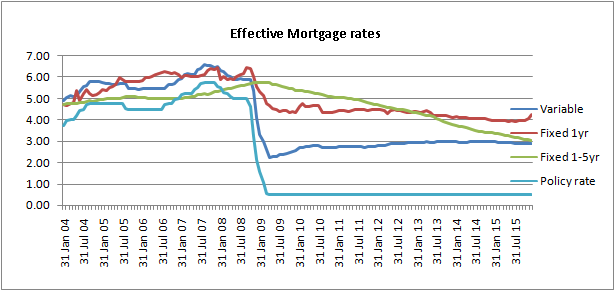
\includegraphics[width=12cm,height=8cm]{mortgage}}
	\subfigure[Corporate lending rates.]{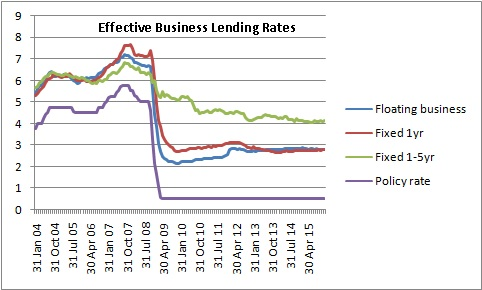
\includegraphics[width=12cm,height=8cm]{busirate}}
\end{figure}



We use the monthly data on effective interest rates (between January 2004 to January 2016)  for mortgage loans in the United Kingdom (for different terms of interest rate fixation) from Bank of England database.
As can be seen in figure below, the response of effective variable interest rate mortgages (to changes in the policy rate) is faster than the effective fixed interest mortgages (as expected).So also the response of the fixed interest mortgages decreases with the increase in the initial term of interest rate fixation.
The effective interest rates for longer term of initial interest rate fixation, change slowly as compared to the shorter term of initial interest rate fixation  because of the fixed nature of the interest rate for the respective term. The effective interest rate implies that a given portfolio of loans has a mix of older loans (which are being repaid over a period of time) which pay interest rate at the interest rates fixed in the past whereas the fresh loans pay interest at the current market rates (depending upon the interest rate pass through). As a result, even if the market interest rates change, the effective interest rates would not change immediately. They change slowly as the older loans are repaid and fresh loans are added to the loan portfolio over a period of time. The same can be observed in the graph for business interest rates

Interest rate stickiness arising due to fixed term loan contracts can vary across different sectors, depending upon the proportion of long term contracts in the portfolio. The following figure presents the effective lending rate for the overall portfolio of all fixed interest loans  (i.e.this includes different fixed term contracts) in case of business loans and mortgage loans. We find that the interest rate pass through is slower for the mortgage loan portfolio as compared to the business loan portfolio due to higher proportion of longer term fixed interest loan contracts.

%\begin{figure}[h!] 
%	\caption{Mortgage lending rates v/s Business lending rates in the UK} 
%	\centering
	
%	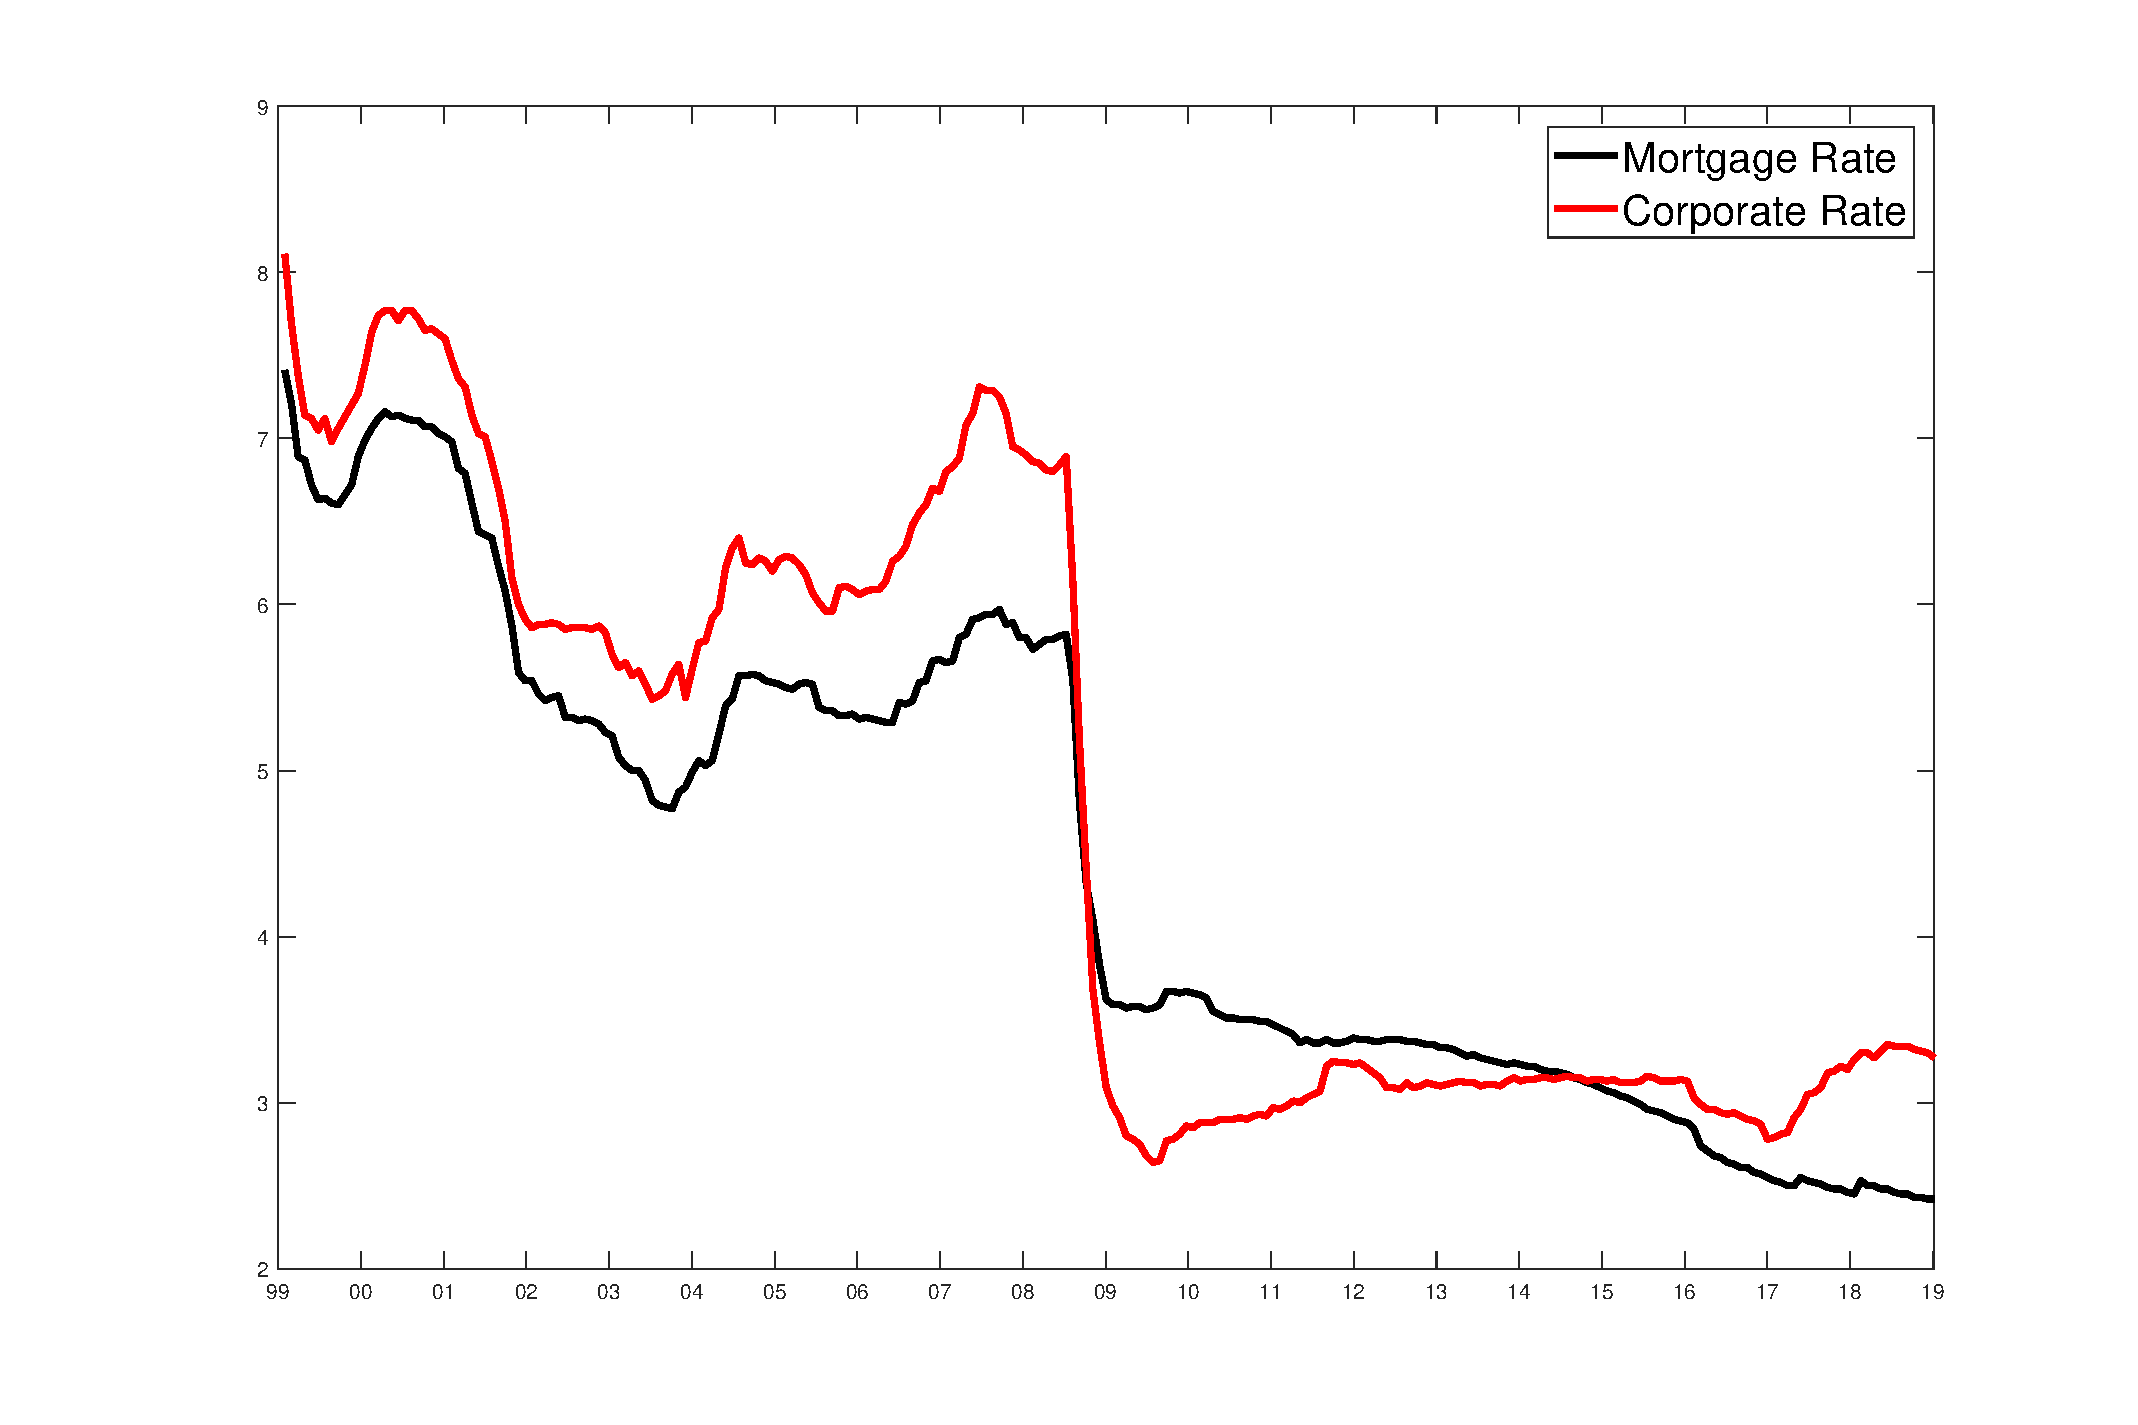
\includegraphics[width=0.9\textwidth]{int_rate_monthly_plot.pdf}
	
%\end{figure}


\subsubsection{Econometric Methodology}


As a first step to investigate the extent of sluggishness in the movement of interest rates, we attempt  to find out how lending rates change in response to change in central bank policy rate.Following the empirical literature on interest rate pass-through models, we run a vector error correction model, where policy interest rates  are considered to be the most direct determinants of retail bank lending rates. We run the following vector error correction model based on Johansen (1991): 

\begin{equation}
{\Delta}R_{t}=\sum _{k=1}^{K }\delta_{k}{\Delta}R^m_{t-k}+\sum _{q=1}^{Q }\gamma_{q}{\Delta}i_{t-q}+\alpha (\mu+R^m_{t}-\beta i_{t})+u_{t}	
\end{equation}

Where $R_{t}$ is the effective lending rate (mortgage loans), $i_{t}$ is the Bank of England policy interest rate,coefficient $\beta$ is the long run equilibrium relationship between bank lending rate and policy rate and the coefficient $\alpha$ is the speed of adjustment of the lending rate to the long run equilibrium. The coefficients of the lags of the first difference of policy rate capture the short-run response of mortgage lending rates to the policy rate. We conduct this exercise for three different lending rates, variable interest rate, fixed interest for a term of up to 1 year and fixed interest rate for a term of 1 to 5 years. Results are summarized in the following table.


\begin {table}[H]
\caption {Regression of UK Bank lending rate on BOE policy rate} \label{tab:title} 
\begin{center}
	\begin{tabular}{||c c c c  ||} 
		\hline
		Regressor & Floating rate & Fixed $<$ 1 year& Fixed 1 to 5 year \\ [0.5ex] 
		\hline\hline
		$\i_{t}$ & $0.016^{***}$ & $0.0057$& $0.0025$ \\ 
		\hline
		$\Delta$ $\i_{t-1}$& $0.896^{***}$ & $0.435^{***}$& $0.018$  \\ 
		\hline
		 $\Delta$ $\i_{t-2}$&$0.016$ & -$0.293^{***}$& -$0.0158$\\
		
		\hline
	$\Delta$ $\i_{t-3}$	&  -$0.008$ & $0.242^{***}$& $0.0097$ \\
		\hline
		$\Delta$  $\i_{t-4}$&-$0.196^{***}$ &-$0.037$& $0.0054$ \\  
		\hline
		constant&$0.1366^{***}$ & - & -\\ 
			
			\hline
		
		\hline
		
	\end{tabular}

\end{center}

\end {table}
\footnotetext{*** is 1 per cent, ** is 5 per cent and * is 10 per cent level of significance }



In case of floating interest rate loans, the response on impact is very low. However,around 90 percent of the pass through takes place in the following month. The above table highlights that the response of floating interest rate to the central bank policy rate, as depicted by coefficients $\{ \i_{t-j} \}_{j=1}^{4}  $,  is higher than the response of 1 year fixed rate loans, which in turn is higher than the response of the 1 to 5 year fixed rate loans.  In case of fixed term of up to 1 year, the response on impact is very low (less than 0.01 percentage point) and around 45 per cent of the pass through takes place in the following month. 


The pass through for the 1 to 5 year fixed term loans is very low. However,there exists a long term co-integration relationship between the two interest rates.For the fixed rate loans, the sum of short run coefficients is less than 1 suggesting an incomplete pass through of policy interest rate.

Thus, the pass through to the fixed interest loans is not only sluggish but also incomplete, whereas the pass through to variable interest loans is faster and almost complete.However, in all the cases including floating interest rate, the response of lending rate on impact is very low (less than 2 percent).

The fact that  floating interest rates adjust faster than the fixed term interest rates,implies that the existence of fixed rate contract is an important source of interest rate sluggishness. So also,the pass through of interest rate changes on impact (i.e. the speed of adjustment) is very small implies that other sources of stickiness such as switching costs, menu costs, market structure/competition, regulation could also be relevant.



 
\section{Model Summary}
Our model closely follows Clerc et. al. (2015), which augments the baseline model of Bernarke, Gilchrist and Gertler (1999) with a detailed banking sector and different types of default on households, corporates and banks to determine the optimal capital adequecy ratio (CAR) for the banking sector, as well as to analyze the macroeconomic implications of bank capital structure under different shocks. 

The BGG framework assumes that interest rates charged by the banks are state contingent. This implies that higher interest rates charged on non-defaulters are sufficient to meet the losses arising from defaulters. This means that banks always make a risk-free return on their investments, which makes the capital structure of the bank irrelevant in the original BGG framework. Clerc et. al. (2015) departs from the BGG framework by assuming a non-contingent lending rate, which implies that in the event of defaults by borrowers, banks may also suffer losses. Therefore, with costly state verification of borrowers, defaults are costly and entail a dead-weight loss for the economy, which necessitates a role for bank capital. They further assume that investor wealth is scarce and hence cost of equity capital is higher than debt funding. This implies that although bank capital is necessary to avoid higher default rates, it is also expensive at the same time, thus creating a trade-off for holding capital. 

Our model deviates from Clerc et. al. (2015) in several important ways. On the banking side, we introduce staggered interest rates à la Calvo (1983) to capture the sluggishness of mortgage and corporate lending rates, which is motivated by the empirical evidence shown in Section 3. Further, we endogenize the bank's capital level by allowing it to be determined in equilibrium through the bank's decision problem. Accordingly, the bank maximizes over its lending rates to households and businesses subject to interest rate sluggishness. The minimum and sectoral capital requirements are introduced as penalty costs on the bank's decision problem, which creates a precautionary motive for the bank to hold a capital level higher than the minimum required. This is a realistic setup since banks typically maintain capital buffers to ensure they do not breach the regulatory minimum. This differs from Clerc et. al. (2015), which assumes that banks always hold the minimum capital requirement\footnote{Another minor deviation in our setup is that there is only one bank in our model than lends corporate and mortgage rates, rather than two sectoral banks as in Clerc et. al. (2015).}. 

On the household and corporate sectors, we introduce an exogenous Loan to Value (LTV) limit on the flow of new lending, which is a key feature of the mortgage and corporate lending sectors. The LTV limits are qualitatively similar to an exogenous collatoral constraint as in Iacoviello (2015). Our main focus in this paper is on the household LTV limit, since the Financial Policy Committee (FPC) in the U.K. does not have such a regulatory tool on corporate lending. Other key distortions and frictions in the model closely follow Clerc et. al. (2015): both the bank and borrowers (mortgage or corporate) in the model are subject to limited liability. The limited liability of banks, along with the presence of a deposit insurance agency implies that banks have an incentive to over-borrow and over-lend, since they do not fully internalize the costs of default. In this framework, regulatory capital is a means to restrict the use of excessive bank leverage. The model further features costly state verification, which implies that the use of leverage is more expensive and that defaults are costly. 

The key agents in the economy are patient and impatient households, entrepreneurs, a bank that lends out in corporate and mortgage sectors, a deposit insurance agency and housing, capital and final goods producers. 


The key agents in the economy are patient and impatient households, entrepreneurs, banks, a deposit insurance agency, housing, \& capital and final goods producers. Figure \ref{model_overview} provides an overview of the main interactions between these agents along with the regulatory tools present in the model. Below we summarize the maximization problems for each agent type, while the associated first-order conditions and further details can be found in Appendix \ref{app_modelOverview}.


\begin{figure}[H]
\caption{An overview of the main actors and regulatory tools in the model.}
\label{model_overview}
	%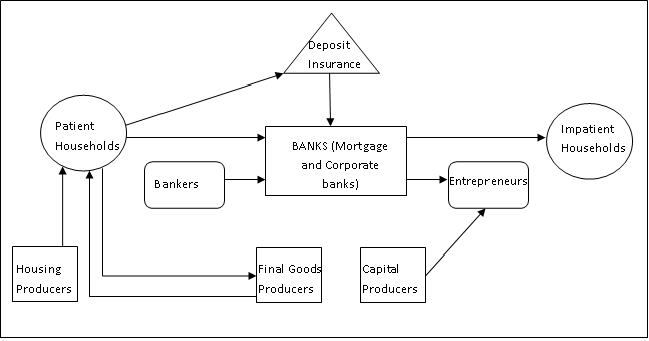
\includegraphics[width=0.9\textwidth]{DIAGRAM1}
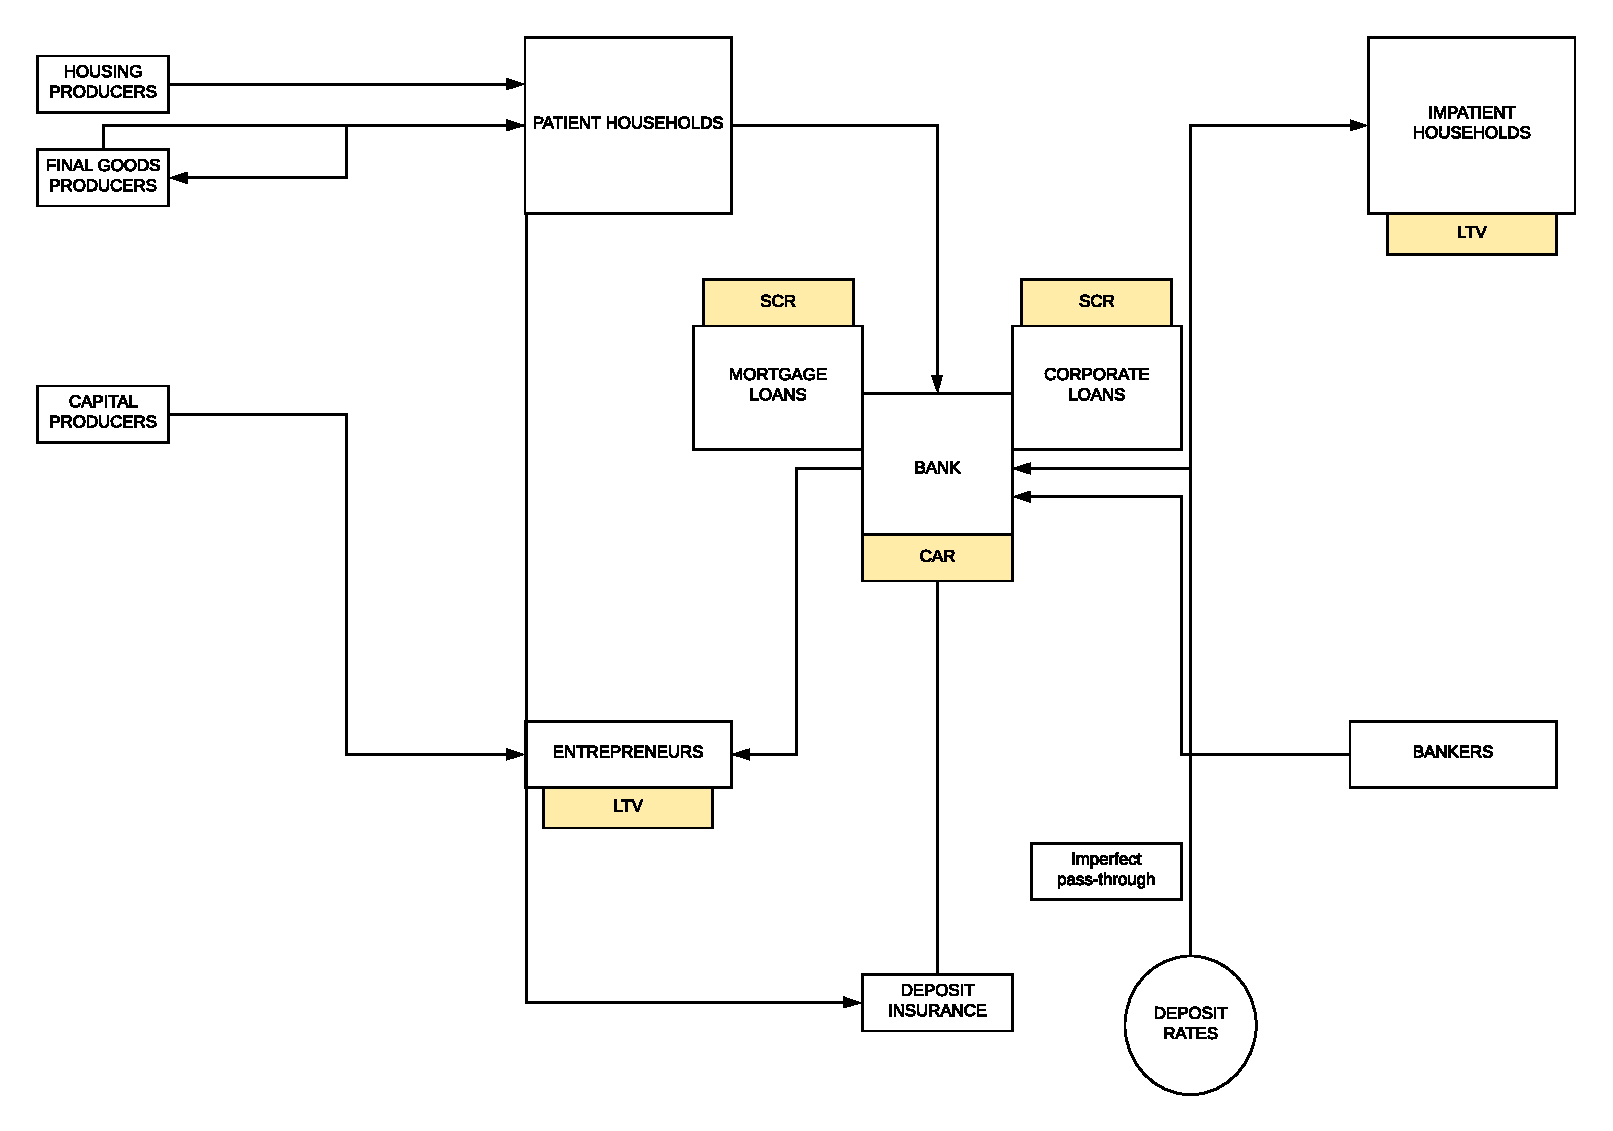
\includegraphics[scale=0.5]{3d_flowchart_prud.pdf}
\end{figure}

\subsection{Overview of Agents}

\noindent
\textbf{Households:} there are two types of households, patient and impatient, with patient households having a higher discount factor as in Iacoviello (2015). Both patient and impatient households have concave utility functions and derive utility from consumption goods, housing and leisure. The individual households are a part of a representative dynasty, which provides perfect risk sharing within the group. Thus, all individual households within the type are ex-ante identical. While the individuals face idiosyncratic shocks, they are perfectly insured within their dynasty and hence consume and save/borrow identically.Both households supply labour in a competitive labour market.

\noindent
\textbf{Patient households} are savers who supply deposits to the bank in equilibrium, and buy houses with their own funds. Both households types derive utility from consumption as well as housing goods, and dis-utility from labour. As such, the patient household's maximization problem is given as:

\begin{equation}
\max_{c^s_t,L^s_t,D_{t},H^s_t}E_t\sum _{t=0}^{\infty } \beta_{s}^t [log(c^s_t)+vlog(H^s_t)-\frac{(L^s_t)^{1+\eta}}{1+\eta} ]
\end{equation}
subject to the following budget constraint: 
\begin{equation}
c^s_t+q^H_{t}H^s_{t} +{D_{t}}=w_{t}L^s_{t}+q^H_{t}H^s_{t-1}(1-\delta)+{D_{t-1}}R^D_{t}+\pi_{t}
\end{equation}

where $\pi_{t}$ includes profits of final goods producing firms and investment \& housing production firms (which are owned by patient households), dividends from entrepreneurs and lump-sum transfers from deposit insurance agency. 



\noindent
\textbf{Impatient households} borrow from banks using their houses as collateral as in Bernanke, Gertler \& Gilchrist (1999). Mortgage loans are made on a limited-liability basis, which implies that individual households can default whenever the value of their house is lower than the outstanding mortgage loans. The value of the house depends both on aggregate shocks, which affect the value of their house, as well as idiosyncratic shocks which affect the default decision of individual borrowers. In equilibrium, borrowers with an idiosyncratic shock below a certain threshold default, in which case the bank takes possession of the house subject to a state verification cost.

We introduce a loan-to-value (LTV) limit set by the macroprudential regulator on the flow of new lending, which is similar to a collateral constraint as in Kiyotaki \& Moore (1997). With the exception of having a different discount factor, the impatient household has the same objective function as the patient household, which is given as follow: 

\begin{equation}
\max_{c^m_t,B^m_t,L_{t},H^m_t}E_t\sum _{t=0}^{\infty } \beta^t_{m} [log(c^m_t)+vlog(H^m_t)-\frac{(L^m_t)^{1+\eta}}{1+\eta} ]
\end{equation}

subject to the following budget constraint, which reflects their borrowings under limited liability: 

\begin{equation}
c^m_t+q^H_{t}H^m_{t} -B^m_{t}=w_{t}L^m_{t}+\int_{\bar{\omega^m_{t} }}^\infty  \left(\omega^m_{t} q^H_{t} H^m_{t-1} (1-\delta)B^m_{t-1}R_{t-1}\right) \, dF\omega^m_{t} + P_{t}
\end{equation}

The term under the integral reflects the limited liability of the borrowers as they default on their loans when the idiosyncratic shock $\omega^m_{t}$ is below the threshold level of $\bar{\omega^m}_t$. The default threshold of the borrowers is determined by: 
%\begin{equation}
%{{\omega^m_{t} }}q^H_{t} H^m_{t-1}(1-\delta) = B^m_{t-1}R^m_{t-1}
%\end{equation}

%The threshold level of $\bar{\omega^m}_t$ satisfies:
\begin{equation}
\bar{\omega^m}_t q^H_{t} H^m_{t-1}(1-\delta) = B^m_{t-1}R^m_{t-1}
\end{equation}


Finally, the LTV limit (or the borrowing constraint) is given by:
\begin{equation}
[B^m_{t}-(1-rp)B^m_{t-1}]R_{t} <=\epsilon_{t} E_t[q^H_{t+1} [H^m_t-H^m_{t-1}(1-\delta)]]
\end{equation}

where rp denotes the loan repayment rate and $\epsilon_{t}$ is the LTV limit. We assume that the LTV limit always binds in the steady state and it's neighbourhood.


\noindent
\textbf{Entrepreneurs } are risk neutral agents who own and maintain the stock of physical capital. They rent  capital to the final goods producing firms. Entrepreneurs derive utility from transferring part of their wealth to the saving dynasty by paying out dividends and retaining the rest for the next period as retained earnings. Entrepreneurs invest in capital goods and finance their investment by means of their own funds, i.e. net worth, and borrowings from banks. Similar to mortgage loans, these are limited liability loans and hence subject to default by individual entrepreneurs in the event of value of assets falling below the value of outstanding loans. The value of the capital depends both on aggregate shocks  as well as idiosyncratic shocks which affect the default decision. In equilibrium, entrepreneurs with an idiosyncratic shock below a certain threshold default.  As in the case of households, assets are seized by banks and subject to costly state verification costs. The entrepreneurs' decision rule is given as follows: 

\begin{equation}
\max_{K_t,B^e_t}E_t(W^e_{t+1})
\end{equation}	

with

\begin{equation}
W^e_{t+1}=max[\omega^e_{t+1}(r^k_{t+1}+(1-\delta)q^K_{t+1}K_{t})-R^F_{t}b^e_{t},0]
\end{equation}


The default decision of the entrepreneurs is determined by: 
%\begin{equation}
%{{\omega^e_{t} }}q^H_{t} K_{t-1}(1-\delta) = K_{t-1}R^f_{t-1}
%\end{equation}

%The threshold level of $\bar{\omega^m}_t$ satisfies:
\begin{equation}
\bar{\omega^e}_t q^K_{t} K^m_{t-1}(1-\delta) = B^e_{t-1}R^f_{t-1}
\end{equation}

Similar to the impatient households, entrepreneurs are subject to the following LTV limit on the flow of new borrowing: 

\begin{equation}
[B^e_t-B^e_{t-1}(1-rp)]R^f_{t} =\epsilon_{t} E_t[q^F_{t+1} [K_t-K_{t-1}(1-\delta)]]
\end{equation}


A fixed proportion of wealth $\chi^e$ is paid out as dividends. This simple dividend paying rule for the entrepreneurs is given by:
\begin{equation}
c^e_t=\chi^e W^e_t
\end{equation}
As a result, the retained earnings by the entrepreneurs is given by:
\begin{equation}
n^e_t=(1-\chi^e) W^e_t
\end{equation}

The balance sheet identity of the entrepreneurs follows as:
\begin{equation}
n^e_t+B^e_t=q^K_t K_t
\end{equation}

\noindent
\textbf{Banks } are financial intermediaries who channel savings from the savers to the borrowers. On the asset side of the banks, there are loans to households (mortgage lending) and entrepreneurs (business lending) respectively. As described earlier, these loans may default depending on aggregate state shocks and idiosyncratic borrower shocks in which case the banks seize the assets subject to state verification costs, which can also be viewed as bankruptcy costs. 


On the liability side of the banks, there are deposits held by the patient households and equity capital held by the bankers. Deposits are insured by the Deposit Insurance Agency (DIA). There is a capital adequacy requirement set by the regulator which, along with a penalty cost function, which determines the amount of equity capital held by the bankers.

One of the key features of the model  is that banks may also default depending on the performance of their loan portfolios, which is driven by aggregate shock, and idiosyncratic shocks similar to the impatient households and entrepreneurs.
 The banks face an idiosyncratic shock to their returns on loans and therefore, in equilibrium, a fraction of banks below a certain threshold of the idiosyncratic shock level default. In case of default, the bank loan assets are possessed by the DIA, subject to costly state verification. 

The banks' balance sheet identity is as follows:
\begin{equation}
n^b_{t}+D_{t}=B^m_{t}+B^e_{t}
\end{equation}


%\hl{we dont have this following  part in the code. This seems to be the old version replaced by 4.22-4.24? Otherwise I don't understand what's going on here. }


\begin{equation}
\resizebox{1\textwidth}{!}{$
	\max_{R^{mi}_t,R^{fi}_t}E_t\sum _{t=0}^{\infty }\xi^t\beta_{s}^t [\{(1-G^H_{t+1}) (\widetilde{R^{mi}_{t}})(B^{mi}_{t})+(1-G^F_{t+1})\widetilde{R^{fi}_{t}}B^{ei}_{t}\}-(1-F^){R^D_{t}}D_{t}+Penalty cost]$}
\end{equation}



\begin{equation}
\widetilde{R^{mi}_{t}}=(1-E_tF^m_{t+1})R^{mi}_t+E_tG^m_{t+1}(1 - \mu^m)( R^{mi}_t/E_t\bar{\omega}^m_{t+1})
\end{equation}
\begin{equation}
\widetilde{R^{fi}_{t}}=(1-E_tF^e_{t+1})R^{fi}_t+E_tG^e_{t+1}(1 - \mu^e)( R^{fi}_t/E_t\bar{\omega}^e_{t+1})
\end{equation}

The demand for Loans is given by:
\begin{equation}
B^{mi}_t=(\frac{R^{mi}_t}{R^{m}_t})^{-\tau} B^{m}_t
\end{equation}

\begin{equation}
B^{ei}_t=(\frac{R^{fi}_t}{R^{f}_t})^{-\tau} B^{e}_t
\end{equation}



%$R^{mi}$ and $R^{fi}$ are the rates of interest that the bank would charge in the absence of interest rate sluggishness. $\tau$ is the elasticity of substitution and determines the market power of the bank, while $\mu$ represent the bankruptcy cost of households and firms respectively. 
%\hl{is this paragraph correct?} 

\textbf{Penalty costs for violating the regulatory requirements}  are modeled as a non-pecuniary gain in utility if the capital adequacy ratio is higher than the minimum capital requirement and a non-pecuniary cost if the capital adequacy ratio is lower than the minimum capital requirement with the following functional form: 

\begin{equation}
PC_t=\nu^b \frac{[\frac{\phi^b_t}{\bar{\varphi_t}}]^{1-\sigma}-1}{{1-\sigma}}
\end{equation}

which is based on Nukhwoon \& Tsomocos (2018). The marginal gains of having excess capital are decreasing, whereas the marginal costs of having a shortfall in capital are increasing, whenever $\sigma$ is greater than 1. This creates an incentive for banks to maintain capital at a higher level than the minimum regulatory requirement. In reality, we find that banks do maintain capital buffer over what is the minimum required, see e.g. Nier and Baumann (2006). The parameter $\nu^b$ determines the weight attached to this penalty costs.


%The above functional form,based on Nukhwoon \& Tsomocos (2018) builds in a non-linearity in the penalty costs.The marginal gains of having excess capital are decreasing whereas the marginal costs of having a shortfall in capital are increasing, whenever $\sigma$ is greater than 1. This creates an incentive for banks to maintain capital at a higher level as compared to the minimum regulatory requirement. In reality, we find that banks do maintain capital buffer over what is the minimum required.The parameter $\nu^b$ determines the weight attached to this penalty costs.

\textbf{Staggered interest rates:} while we find that one of the main sources of interest rate stickiness is the existence of fixed-interest rate loans as shown by our empirical exercise in Section 3, interest rate stickiness can be attributed to various reasons such as switching or menu costs, market structure, regulation and so on. Therefore we introduce interest rate stickiness in a broader sense by modeling it as in Calvo (1983). This approach has the benefit of including all possible sources of interest rate stickiness in a reduced form. As such, we assume that only a proportion of 1-$\xi$ of banks are able to change their lending rates in a given period, whereas the remaining proportion $\xi$ are unable to change their lending rate, which remains fixed at previous period's value. Accordingly, the composite interest rate in the economy is a weighted average of the current interest rate charged by the banks that can change their interest rate, and the previous period's interest rate used by the banks that cannot change their interest rate. 

In order to micro-found the staggered interest rate setting, we assume that there is imperfect competition in the banking sector, where banks offer differentiated loan products as in Gerali et. al. (2010) and are able to set their interest rate in the monopolistically competitive loan market. The borrowers then take a composite loan product consisting of these differentiated banking services. The first-order conditions of the bank for interest rates resemble the first-order conditions for prices in a standard New Keynesian setting with price stickiness, and they are given as: 


%To micro-found the staggered interest rate setting, we assume that there is imperfect competition in the banking sector. Banks offer differentiated loan products as in Gerali et al (2010) and are able to set their interest rate in the monopolistically competitive loan market.The borrowers takes a composite loan product comprising of all the aforesaid differentiated banking services.The composite interest rate paid by the borrowers is thus staggered on account of the Calco friction.In short,we extend the New Keynesian approach to goods market to the loan markets so as to generate interest rate stickiness. 
%The FOCs for the interest rates are as follows.The FOC is similar to the FOC for price in a standard New Keynesian model with goods price stickiness:

\begin{equation}
R^{mi}_t=\frac{\tau}{\tau-1}\frac{E_t\sum _{t=0}^{\infty }\xi^t\beta_{s}^t MC_t}{E_t\sum _{t=0}^{\infty }\xi^t\beta_{s}^t rm_t}
\end{equation}
\begin{equation}
R^{fi}_t=\frac{\tau}{\tau-1}\frac{E_t\sum _{t=0}^{\infty }\xi^t\beta_{s}^t MC_t}{E_t\sum _{t=0}^{\infty }\xi^t\beta_{s}^t rf_t}
\end{equation}

\begin{equation}
MC_t=\lambda_{st+1}[(1-F^B_t)R_{Dt}+\frac{\nu^b(\phi^b_t/{\bar{\varphi_t}})^{(1-\sigma)}}{(B^{mi}_t+B^{ei}_t)}](R^m_t)^\tau B^m_t
\end{equation}

where the interest rate charged by banks is a function of present discounted value of present and future "marginal cost" (MC) times the mark-up, where the MC includes the interest rate paid on deposits in a competitive deposit market, and the penalty cost associated with deviating from regulatory capital requirements.  
% The only difference from the standard New Keynesian version is the presence of borrower and bank defaults in the interest FOC for interest rate equation
%As in the New Keynesian model with price stickiness, the interest rate charged by banks is a function of present discounted value (with the stickiness parameter) of present and future marginal cost times the mark up. The marginal cost includes the interest rate paid on deposits (in a competitive deposit market) and the penalty cost associated with the deviation from the regulatory capital requirement.
\textbf{Deposit Insurance Agency} insures the deposits, where the assets of the defaulting banks are taken over by the agency and are subject to bankruptcy costs. The difference between the amount of deposits and the value of realized assets is recovered by imposing a lump-sum tax on households. 

\textbf{Final goods producing firms} are modeled as a unit mass of perfectly competitive firms, which combine capital and labor to produce the consumption good. The firms rent capital from entrepreneurs, and they are owned by patient households. They produce the final goods using a standard Cobb-Douglas technology: 

\begin{equation}
Y_{t}=E_{A_{t}} K^{\alpha}_{t-1}L^{1-\alpha}_{t}
\end{equation}

\textbf{Capital goods and housing production } comes from competitive firms, owned by patient households,  that buy finished goods and produce capital goods and housing subject to quadratic adjustment costs. These firms produce new units of capital and housing using consumption goods, which are then sold to entrepreneurs and households. As such, they represent the supply side of capital goods and housing, and they pin down the equilibrium asset prices. 

\subsection{Exogenous Processes}

The model is equipped with 12 exogenous AR(1) processes across different sectors. On the housing side, we have two preference shocks on housing and consumption $E_{J,t}$ and $E_{C_t}$, which affect the taste of both patient and impatient households for consumption and housing goods respectively. These shocks can be equivalently interpreted as the degree of risk aversion to purchasing consumption and housing goods. We further have a housing price shocks $E_{H,t}$, which is an external shock that directly affects the housing price index\footnote{This shock can also be thought of as a measurement error, i.e. the component of the housing prices that is not explained internally by the model.}. Finally, we have a shock on the LTV limit of the households, $E_{LTVH,t}$ which is introduced in order to relax the restrictiveness of an always binding constraint. 

On the corporate side, we have a net worth shock $E_{We,t}$, which is a transfer from the housing sector to the businesses, which we use as a proxy for an exogenous government spending shock in our model. We also introduce a risk shock $E_{Se,t}$ into the corporate sector, which affects businesses' likelihood of default. Finally, we have an expected capital price shock $E_{EbF,t}$, which drives the stock market sentiment in the model. 

On the banking side, we have bank risk shock $E_{Sb,t}$ that has a similar meaning  as tis counterpart in the corporate sector. The bank is further subject to a bank capital shock $E_{CAB,t}$, affect its capital ratio, and two mark-up shocks on its interest rate setting $E_{markup^m,t}$ and $E_{markup^F,t}$, which affect the cost of mortgage and corporate lending respectively for the bank. These mark-up or cost-push shocks help introduce a wedge between the realized interest rates and the rates that the bank would use in the absence of interest rate stickiness. 

Finally, the Cobb-Douglas production function of final goods producing firms is subject to a productivity shock $E_{A,t}$\footnote{We also experimented with different combinations of shocks across different sectors, e.g. a risk shock on the housing sector, an LTV limit shock on the corporate sector, housing and capital depreciation shocks and a net worth shock in the banking sector. The particular set of shocks reported in the paper emerges as the best combination of shocks in terms of model likelihood and providing a reasonable historical variance decomposition for key variables.}. 



%housing: depreciation, uncertainty, preference shocks (4)
%corporate: depreciation, uncertainty, net worth (3)(
%banking: uncertainty, markups, bank capital, net worth (4)
%aggregate: productivity (1)



%The model is equipped with 13 shocks: \\
%-Productivity shock on output, $A_t$\\
%-Housing and capital depreciation shocks, $Hd_t$ and $Hk_t$. These are shocks directly affecting the depreciation rates of housing and capital stocks. Therefore a positive shock directly translates into a reduced stock of housing or capital owned by households, and therefore a lower rate of return on housing or capital. \\
%-Risk (uncertainty) shocks on Entrepreneurs $Se_t$, impatient households $Sm_t$ and the bank $SB_t$. These shocks affect the volatility of default rates for the associated agents. In other words, these shocks are changes in the volatility of cross-sectional idiosyncratic uncertainty. A larger volatility implies a larger number of agents falling below their default threshold, therefore larger risk shocks directly translate into higher default rates.  \\
%-Net worth shocks on corporates and the bank, $Wb_t$ and $We_t$: since the bank and the business are owned by patient households, these shocks translate into budget constraint shocks on the patient households. \\
%-Household preference shocks $J_t$ and $EC_t$. These are shocks on the household and consumption preference of both types of households. A negative household or consumption shock means less purchasing of that commodity type, therefore they can be equivalently interpreted as risk aversion shocks to the given commodity type. \\
%-Bank capital shock $CAB_t$: this is a shock directly affecting the capital ratio of the bank. In the absence of a monetary policy authority, these shocks can be interpreted as a proxy for monetary policy shocks. \\
%-Markup, or cost-push shocks $H_{markup,t}$ and $F_{markup,t}$: these are shocks on the mortgage and corporate rate that the bank would like to set. An increase in either shock can be interpreted as an external factor that pushes up the bank's cost of lending, which results in an increase in the rate that the would set in the absence of sluggishness. As such, these are shocks to the wedge interest rate wedge driven by stickiness.

\section{Estimation}



\subsection{Measurement equations} 

We use quarterly data from U.K. over the period $1998Q1-2016Q2$ for ten key macroeconomic and financial variables\footnote{Further details on the observable variables can be found in the appendix.} for the Bayesian estimation of our model\footnote{The preceding two years over 1996Q1-1997Q4 are used as a training sample.}. For aggregate output $Y_t$, wages $W_t$, investment $I_t$, consumption $C_t$, as well as House prices $q^{H,t}$, corporate lending $b_{e,t}$ and mortgage lending $b_{m,t}$, we match the data in terms of growth rates with a measurement equation of the form: 

\begin{equation}
\Delta x_t^{obs}=\gamma_x+ X_t-X_{t-1},
\end{equation}

with $x \in \{Y, W, I, C, q^{H}, b_e, b_m \} $, where $\gamma_x$ denotes the historical average of each time series under consideration\footnote{Since our model does not feature a steady-state growth, these averages are pre-computed and remain fixed during the estimation.}. For the remaining three variables, namely the official bank rate $R^{D}_{t}$, the effective mortgage lending rate $R^H_t$ and the effective corporate lending rate $R^m_t$, we match the data in levels with a measurement equation of the form: 

\begin{equation}
y_t^{obs}=100(\bar{Y}-1) + Y_t,
\end{equation}

with $y \in \{R^D, R^H, R^m \}$ and $\bar{Y}$, and $\bar{Y}$ denotes the steady-state level of the associated variables in the model. Note that we match the official bank rate to the deposit rates in the model\footnote{An alternative approach is to use both the official bank rate and average deposit rates, where the difference between the two is captured with another layor of staggered interest rates. This approach has been adopted in Paries et. al. (2010), where they find little evidence of staggered rates between these two time series. Therefore in this paper, we directly equate the deposit rates to the official bank rate for simplicity.}. 



$\gamma_Y,\gamma_W,\gamma_I,\gamma_C,\gamma_{\Delta q^H} $ and $\gamma_{\Delta b}$ are obtained by demeaning the series prior to estimation, since our model does not feature steady-state growth. $\bar{R^H}, \bar{R^m}$ and $\bar{R^D}$\footnote{We assume that the deposit rates are equivalent to the official Bank Rate in our estimation exercise since there is no monetary policy in our model. In the presence of monetary policy, an alternative would be to introduce another layer of sluggishness from the Bank Rate to deposit rates. However, Pariès et. al. (2010) find little evidence for the importance of this channel based on EU data.} denote the gross lending and deposit rates at the steady-state of the model.  

\subsection{Calibrated Parameters and Prior Distributions }

Prior to estimation, we fix a number of parameters by either following conventional values used in the literature or to generate steady-state values consistent with U.K. data. Parameters relating to default costs are based on Mendicino et. al. (2015): the depositor cost of bank default $\gamma$ is fixed at $0.1$. The bankruptcy cost of households, businesses and banks $\mu_m, \mu_e$ and $\mu_B$ are set to a common value of $0.3$. The discount factor for patient households is $0.995$. 


For some parameters, we use standard values following convention in the literature. Accordingly, capital share in production is set to $0.3$, while the Frisch elasticity of labor $\eta$ is $1$. The labor preference parameters for both types of households $\varphi_s$ and $\varphi_m$ are normalized to $1$ since they mainly scale the size of the economy. The parameters $a_s$ and $a_b$ are set to $0.5$, which determine the share of total default costs paid by saving and borrowing households respectively. 


Some parameters are closely linked with the steady-state of the economy. We use these parameters to generate plausible ratios for some of the key variables. The housing preference parameters for both types of households, $v_s$ and $v_m$, as well as business and bank dividend payout parameters, $\chi_e$ and $\chi_b$, are used to generate plausible business and mortgage lending to aggregate output ratios.  Accordingly, we set $v_s=0.25$ and $v_m=0.5$, while the divident payouts are set to $\chi_e=0.1$ and $\chi_b=0.15$. These generate lending ratios of $133 \%$ and $86 \%$ for corporate and mortgage lending to output respectively, which are reasonably close to the historical means of the corresponding U.K. ratios over the estimation period, which are $118 \%$ and $81 \%$ respectively. At the given values, mortgage lending constitutes $38 \%$ of total lending in steady-state. Similarly, we set the housing and capital depreciation rates to $\delta_H=0.01$ and $\delta_K=0.04$, which yields an investment to output ratio of $12 \%$, which is close to the historical mean of $17 \%$ for the U.K. economy over this period\footnote{In the model, aggregate investment is calculated as the sum of housing and capital investment. The historical mean ratio for the U.K. is taken from ons.gov.uk for the estimation period.}. The parameters determining market power of the bank, $\tau_m$ and $\tau_F$ are both set to 40, whereas the hyperparameters in the cost function are set to $\psi_b=5$ and $\nu=0.5$. Finally, we set the household and entrepreneur repayment rates in the LTV limit as $0.01$ and $0.05$ respectively. 

Parameters relating to macroprudential regulation are fixed in our benchmark estimations. Accordingly, for minumum capital requirements, we use a benchmark value of $\phi_H=\phi_F=0.11$ for both sectors, which is close to the historical minimum capital requirements for U.K\footnote{Available data for capital requirements is taken from Bank of England's website, where we use Basel III common equity Tier I capital ratio after 2014, and Core Tier I capital ratio before 2014. Alternatively, one could use the capital requiments as another observable in the estimation, but we choose to fix these ratios given that Basel requirements do not have a one-to-one correspondence in the model, and that the data is only available at an annual frequency before 2014.}. We assume that there is no CCyB in place in our benchmark estimations, and the LTV limit for households is fixed at 86 \%, which corresponds to the historical average over most of this period for the U.K. economy\footnote{Similar to capital ratios, the data to calculate this average is taken from BoE's website, where we use the Residential mortgage LTV ratio, available over the period 2005-2016.}. We fix the LTV limit on corporates at the same value as household LTV, since the FPC in the U.K. does not have such a regulatory tool. 


The remaining 33 parameters are estimated using Bayesian likelihood methods to match the data. For the AR(1) coefficients of all exogenous shocks, we use a standard Beta distribution with mean $0.5$ and standard deviation $0.2$ following Smets-Wouters (2007) . The standard deviations of all exogenous shocks are assigned a diffuse uniform prior over the interval $[0,10]$. The volatility of i.i.d. shocks on households, businesses and banks follow a common Inverted Gamma distribution with mean $0.1$ and standard deviation $2$: we choose to use more informative priors for these parameters since both aggregate and i.i.d shocks mainly relate to the level of default rates in a first-order approximation, hence estimating both sets of parameters with uninformative priors may lead to identification issues. For the cost adjustment parameters $\psi_i$ and $\psi_h$, we assume a conventional normal distribution with a mean of $5$ and standard deviation $2$\footnote{See e.g. Smets-Wouters (2007), which uses a normal prior with mean 4 and standard deviation 1.5. Note that our prior is more diffuse compared to BoE's COMPASS model (2013), which uses a tight Gamma prior with mean $2$ and standard deviation $0.4$.}. For habit formation $\lambda$, we use the same Beta prior as in Calvo parameters, and for the impatient household discount factor $\beta_m$, we use a tight Beta prior with $0.98$ and standard deviation $0.01$ to ensure that the prior interval for this parameter remains below the patient household discount factor of $0.995$. Finally, the volatility of the default shock parameters $\sigma_e$, $\sigma_m$ and $\sigma_B$ are assigned inverted Gamma priors with mean $0.1$ and standard deviation 2\footnote{These i.i.d. essentially play the same role as the exogenous risk shocks in terms of determining the default rates (with the difference that i.i.d. shocks affect the steady-state levels, while the exogenous shocks do not). Therefore these two sets of shocks may not be jointly identified, therefore we assign more informative priors for these parameters compared to the standard deviation of exogenous shocks.}. The priors for all parameters are summarized in Table \ref{post_dist}. 

The steady-state of our model is not available in closed-form and therefore it is numerically computed for every parameter draw. This increases the computational burden associated with the posterior distributions. This complicates the estimation of parameters that affect the steady-state, namely the habit formation, impatient household discount rate, and the i.i.d. shock variances. Therefore for five these parameters, we only compute the point estimates for the candidate density (i.e. posterior mode). We then leave the parameters fixed at these point estimates before proceeding to the computation of posterior distributions\footnote{Alternatively one could fix these parameters similar to the others, but we did not find studies with similar parameters on the U.K. data that could guide the choice of these and therefore took this intermediate approach.}.  

The posterior distributions of the remaining 28 parameters are computed using 4 parallel Monte Carlo Markov Chains (MCMC), each with 500000 draws where the first half of each chain is discarded as a burn-in sample. The scaling coefficient of the parameter covariance matrix is adjusted to obtain an acceptance ratio of around $35 \%$ in each case. 
 

\begin{comment} 
\begin{table}[H]
\caption{Prior Distributions}
\begin{tabular}{l|l|l|l}
Parameter & Prior &  &  \\
\hline
\hline
 & Dist & Mean & Variance \\
 \hline
\hline
$\epsilon_{A}$ & Uniform & 10 & 5.77 \\
$\epsilon_{J}$ & Uniform & 10 & 5.77 \\
$\epsilon_{H}$ & Uniform & 10 & 5.77 \\
$\epsilon_{Se}$ & Uniform & 10 & 5.77 \\
$\epsilon_{SB}$ & Uniform & 10 & 5.77 \\
$\epsilon_{We}$ & Uniform & 10 & 5.77 \\
$\epsilon_{markup_m}$ & Uniform & 10 & 5.77 \\
$\epsilon_{markup_e}$ & Uniform & 10 & 5.77 \\
$\epsilon_{EC}$ & Uniform & 10 & 5.77 \\
$\epsilon_{ECAB}$ & Uniform & 10 & 5.77 \\
$\epsilon_{LTVH}$ & Uniform & 10 & 5.77 \\
$\epsilon_{EbF}$ & Uniform & 10 & 5.77 \\


$\rho_{A}$ & Beta & 0.5 & 0.2 \\
$\rho_{J}$ & Beta & 0.5 & 0.2 \\
$\rho_{H}$ & Beta & 0.5 & 0.2 \\
$\rho_{Se}$ & Beta & 0.5 & 0.2 \\
$\rho_{SB}$ & Beta & 0.5 & 0.2 \\
$\rho_{We}$ & Beta & 0.5 & 0.2 \\
$\rho_{markup_m}$ & Beta & 0.5 & 0.2 \\
$\rho_{markup_e}$ & Beta & 0.5 & 0.2 \\
$\rho_{EC}$ & Beta & 0.5 & 0.2 \\
$\rho_{ECAB}$ & Beta & 0.5 & 0.2 \\
$\rho_{LTVH}$ & Beta & 0.5 & 0.2 \\
$\rho_{EbF}$ & Beta & 0.5 & 0.2 \\

$\phi_i$ 	  &   Normal   &  4   & 1.5    \\
$\phi_h$ 	  &   Normal  &   4   & 1.5  \\

$\zeta_m$ & Beta & 0.5 & 0.2 \\
$\zeta_e$ & Beta & 0.5 & 0.2 \\

$\beta_m$ 	  &   Beta   &  0.98   & 0.01    \\
$\lambda$ 	  &  Beta    &   0.5  &   0.2  \\

$\sigma_e$ & Inv. Gamma & 2 & 0.1 \\

$\sigma_m$ & Inv. Gamma & 2 & 0.1 \\

$\sigma_B$ & Inv. Gamma & 2 & 0.1 \\
\end{tabular}
\end{table}
\end{comment}


\subsection{Posterior Distributions for Estimated Parameters}

The point estimates, along with the 95 \% highest posterior density (HPD) intervals for the parameters are reported in Table \ref{post_dist}\footnote{The distributions of all estimated parameters can be found in Appendix \ref{app_posteriorDist} in Figures \ref{app_post1} and \ref{app_post2}.}. Of particular interest are Calvo parameters, for which the posterior distributions are along with the posterior mean and mode are shown in Figure \ref{post_calvo}. We find a Calvo probability of 49.7 \% for corporate rates, whereas the probability for mortgage rates is 71.8 \%. This means, on average, banks are able to reset the interest rates on corporate loans once every 1.98 quarters or 5.94 months, while it takes much longer to reset the interest rates on mortgage loans with an average duration of 3.54 quarters or 10.62 months. The 95 \% credible intervals are $[5.19, 6.51]$ for corporate rates and $[8.82,12.48]$ for mortgage rates. The shocks are typically estimated with high autocorrelation coefficients, with the exception of bank and entrepreneur risk shocks. In particular, the productivity, housing preference and business net worth shocks have autocorrelation coefficients near unity, implying high persistence. These shocks also emerge as the main drivers of the business cycle for key variables as will be discussed below. For the capital and housing investment adjustment cost parameters, we find values of $7.92$ and $4.85$ respectively, implying more sluggishnes in housing investment compared with capital investment. 



\begin{table}[H]
\caption{Posterior Estimates}
\label{post_dist}
\begin{tabular}{l||lll|llll}
\textbf{Parameter} & \textbf{Prior} & &  & \textbf{Posterior} &  &  &  \\
 & Dist & Mean & Variance & Mode & Mean & HPD \% 5 & HPD \% 95 \\
 \hline
 \hline
 $\epsilon_{A}$& Uniform & 10 & 5.77 & 0.0078 & 0.0079 & 0.0068 & 0.0092 \\
 $\epsilon_{J}$& Uniform & 10 & 5.77 & 0.0971 & 0.1019 & 0.0841 & 0.1234 \\
$\epsilon_{H}$ & Uniform & 10 & 5.77 & 0.0396 & 0.0499 & 0.0323 & 0.0739 \\
$\epsilon_{Se}$ & Uniform & 10 & 5.77 &0.0462 & 0.0728 & 0.0317 & 0.1483 \\
$\epsilon_{SB}$ & Uniform & 10 & 5.77 & 0.0308 & 0.0317 & 0.0244 & 0.0398 \\
$\epsilon_{We}$ & Uniform & 10 & 5.77 & 0.0053 & 0.0055 & 0.0047 & 0.0064 \\
$\epsilon_{markup_m}$ & Uniform & 10 & 5.77 & 0.0005 & 0.0005 & 0.0004 & 0.0006 \\
$\epsilon_{markup_e}$ & Uniform & 10 & 5.77 & 0.0004 & 0.0004 & 0.0003 & 0.0004 \\
$\epsilon_{EC}$ & Uniform & 10 & 5.77 & 0.0288 & 0.0295 & 0.0253 & 0.0341 \\
$\epsilon_{ECAB}$ & Uniform & 10 & 5.77 & 0.0379 & 0.038 & 0.029 & 0.0486 \\
$\epsilon_{LTVH}$ & Uniform & 10 & 5.77 &0.1353 & 0.1563 & 0.1105 & 0.208 \\
$\epsilon_{EbF}$ & Uniform & 10 & 5.77 & 0.0423 & 0.0435 & 0.0369 & 0.0516 \\
\hline
$\rho_{A}$ & Beta & 0.5 & 0.2 & 0.9956 & 0.9905 & 0.9786 & 0.9978 \\
 $\rho_{J}$ & Beta & 0.5 & 0.2 & 0.9849 & 0.9836 & 0.9733 & 0.9919 \\
$\rho_{H}$& Beta & 0.5 & 0.2 & 0.9572 & 0.9416 & 0.9051 & 0.9723 \\
$\rho_{Se}$ & Beta & 0.5 & 0.2 & 0.499 & 0.4983 & 0.1723 & 0.8312 \\
$\rho_{SB}$ & Beta & 0.5 & 0.2 &0.0328 & 0.0498 & 0.0143 & 0.0984 \\
$\rho_{We}$ & Beta & 0.5 & 0.2 &0.8434 & 0.835 & 0.7663 & 0.8981 \\
$\rho_{markup_m}$  & Beta & 0.5 & 0.2 & 0.8717 & 0.8685 & 0.7839 & 0.9447 \\
$\rho_{markup_e}$ & Beta & 0.5 & 0.2 &0.9347 & 0.9304 & 0.8851 & 0.969 \\
$\rho_{EC}$ & Beta & 0.5 & 0.2 & 0.8424 & 0.8433 & 0.8012 & 0.8787 \\
$\rho_{ECAB}$ &Beta & 0.5 & 0.2 &0.9268 & 0.9194 & 0.8675 & 0.9678 \\
$\rho_{LTVH}$ & Beta & 0.5 & 0.2 & 0.9292 & 0.9082 & 0.8207 & 0.971 \\
$\rho_{Wb}$ & Beta & 0.5 & 0.2 & 0.9733 & 0.9587 & 0.9008 & 0.9907 \\
\hline
$\psi_i$ &    Normal   &  4   & 1.5  & 7.9159 & 8.0655 & 5.7808 & 10.5123 \\
$\psi_h$ &    Normal   &  4   & 1.5  & 4.8532 & 5.821 & 3.5007 & 8.4709 \\
$\zeta_m$ & Beta & 0.5 & 0.2 & 0.7179 & 0.7155 & 0.6629 & 0.7607 \\
$\zeta_e$ & Beta & 0.5 & 0.2 & 0.4967 & 0.4914 & 0.4333 & 0.5468 \\
\hline
$\beta_m$ & Beta   &  0.98   & 0.01  & 0.9719 & - & - & - \\
$\lambda$ & Beta    &   0.5  &   0.2  & 0.6626 & - & - & - \\
$\sigma_e$  & Inv. Gamma & 2 & 0.1 & 0.0802 & - & - & - \\
$\sigma_m$ & Inv. Gamma & 2 & 0.1  & 0.0915 & - & - & - \\
$\sigma_B$ & Inv. Gamma & 2 & 0.1  & 0.0751 & - & - & - \\

\end{tabular}
\end{table}




\begin{figure}[H]
\centering
\caption{Posterior distributions of estimated Calvo parameters on interest rate setting.}
\label{post_calvo}
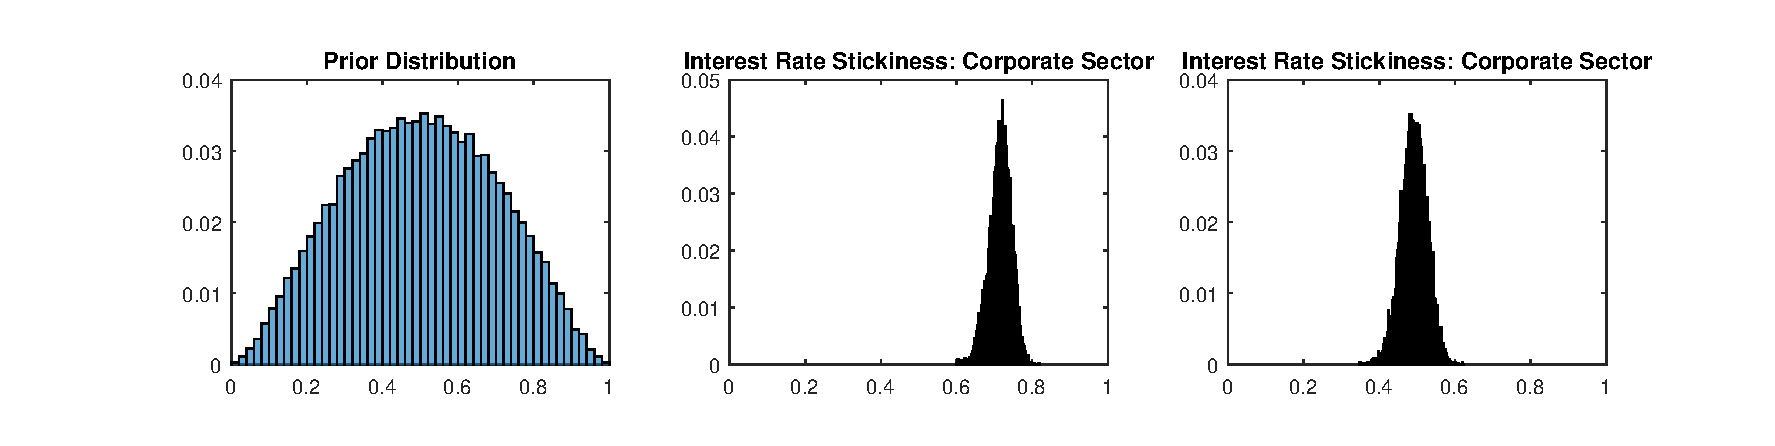
\includegraphics[scale=0.65]{posteriordistributions_calvo2.pdf}
\end{figure}

\FloatBarrier

\subsection{Estimated Shocks}

Figure \ref{estimated_shocks} shows some of the key estimated shocks along with their 95 \% HPD intervals\footnote{The full set of shocks, along with all of the observable variables are reported in Appendix \ref{app_dataAndShocks}. } over our sample period, which illustrates which shocks play a dominant role during the financial crisis period. Accordingly, it takes the combination of several adverse shocks to generate the crisis in the model. On the housing side, the main drivers emerge as the housing preference and housing price shocks as both of them fall considerably around the crisis period\footnote{We tested alternative version of the model with depreciation and expected price shocks on the housing side, in which case the role played by the preference and house price shocks are somewhat reduced.}. The house price shock in our model plays a qualitatively similar role to a measurement error, i.e. it is an external shock that directly hits the house price level. Keeping everything else equal, the effect of such a drop in housing prices is to boost housing demand and investment. Therefore, the adverse effects of the house price drop on output growth and the macroeconomy as a whole are picked up by the housing preference shock. Similar to the housing shocks, there is a sizeable drop in the consumption preference shock, which slowly starts to pick up after the crisis but remains persistently low throught the sample period. The drop in consumption preference helps explain the reduction in consumption growth and, as a result, in output growth. Given the similar patterns in housing and preference shocks, these two simultaneous drops can be interpreted as an increased risk aversion to spending by households\footnote{Note that there is also a substitution effect at play with these two preference shocks: since both prefence shocks leave the household wealth unchanged, a negative consumption preference shock increases housing demand whereas a negative housing preference shock increases consumption spending.}. 

On the business side, the entrepreneur and expected capital price shocks play a dominant role compared to the rest. The entrepreneur net worth shock decreases during the crisis but quickly picks up afterwards, while the expected capital price shock gradually decreases after the crisis. The entrepreneur net worth shock plays a particularly important role in driving output growth as we will discuss below. This shock has a redistributional effect from households to the corporate sector, and as such we interpret it as picking up the effects of an external government spending shock in our framework. It is important to note that this shock remains elevated during the post-crisis period compared to its values during early 2000s. 

Finally, the productivity shock decreases during the crisis period. We observe a pattern in the productivity process similar (but opposite of) to the entrepreneur net worth shock, where the productivity process not does recover after the crisis period and remains lower compared to its pre-crisis level. The post-crisis lower productivity is consistent with the conventional wisdom surrounding productivity in the U.K. 

The remaining shocks (not reported in Figure \ref{estimated_shocks}) play a smaller degree during the crisis period and over the business cycle as a whole: the mortgage and corporate loan mark-up shocks are typically small with the exception of when interest rates fall to the zero lower bound levels. This corresponds to the period where the gap between the official bank rate and the mortgage \& corporate loans grows. Accordingly, these two shocks help generate the interest rate stickiness and obtain the Calvo probabilities reported in the previous section. The bank net worth and bank capital shocks also play a surprisingly small role especially surrounding the crisis period. Finally the housing LTV shock decreases once the adverse shocks hit, which is interpreted as the borrowing constraint becoming more restrictive during this period. However, this shock does not play a substantial role in the variance decompositions as will be discussed below. 


Figure \ref{estimated_shocks}b shows the estimated default rates across all three sectors. It is readily seen that corporate default rates remain practically at zero throughout the sample period, implying this layer of default does not play an important role. The bank default rate is somewhat increased during the crisis period, although it still remains at low levels throughout the sample\footnote{We experimented with an alternative version of the model, where we use the average price-to-book ratio of U.K. banks as a proxy for the AR(1) bank risk shock, which directly determines the bank default rate in the model. In this case we obtain a sharper jump in the bank default rate during the crisis, but the overall default rate as well as the wider implications for the model remain qualitatively the same.}. Unlike the bank and corporate default rates, the household default rate is substantially increased during the crisis period, and it remains elevated until 2012 before starting to come down. Together with the redistributional entrepreneur net worth shock, this increase in the default rate can be interpreted as households paying the cost of the crisis. 



\begin{figure}[H]
\centering
\caption{Estimated Shocks and Default Rates over 1998Q1-2016Q2.}
\label{estimated_shocks}
%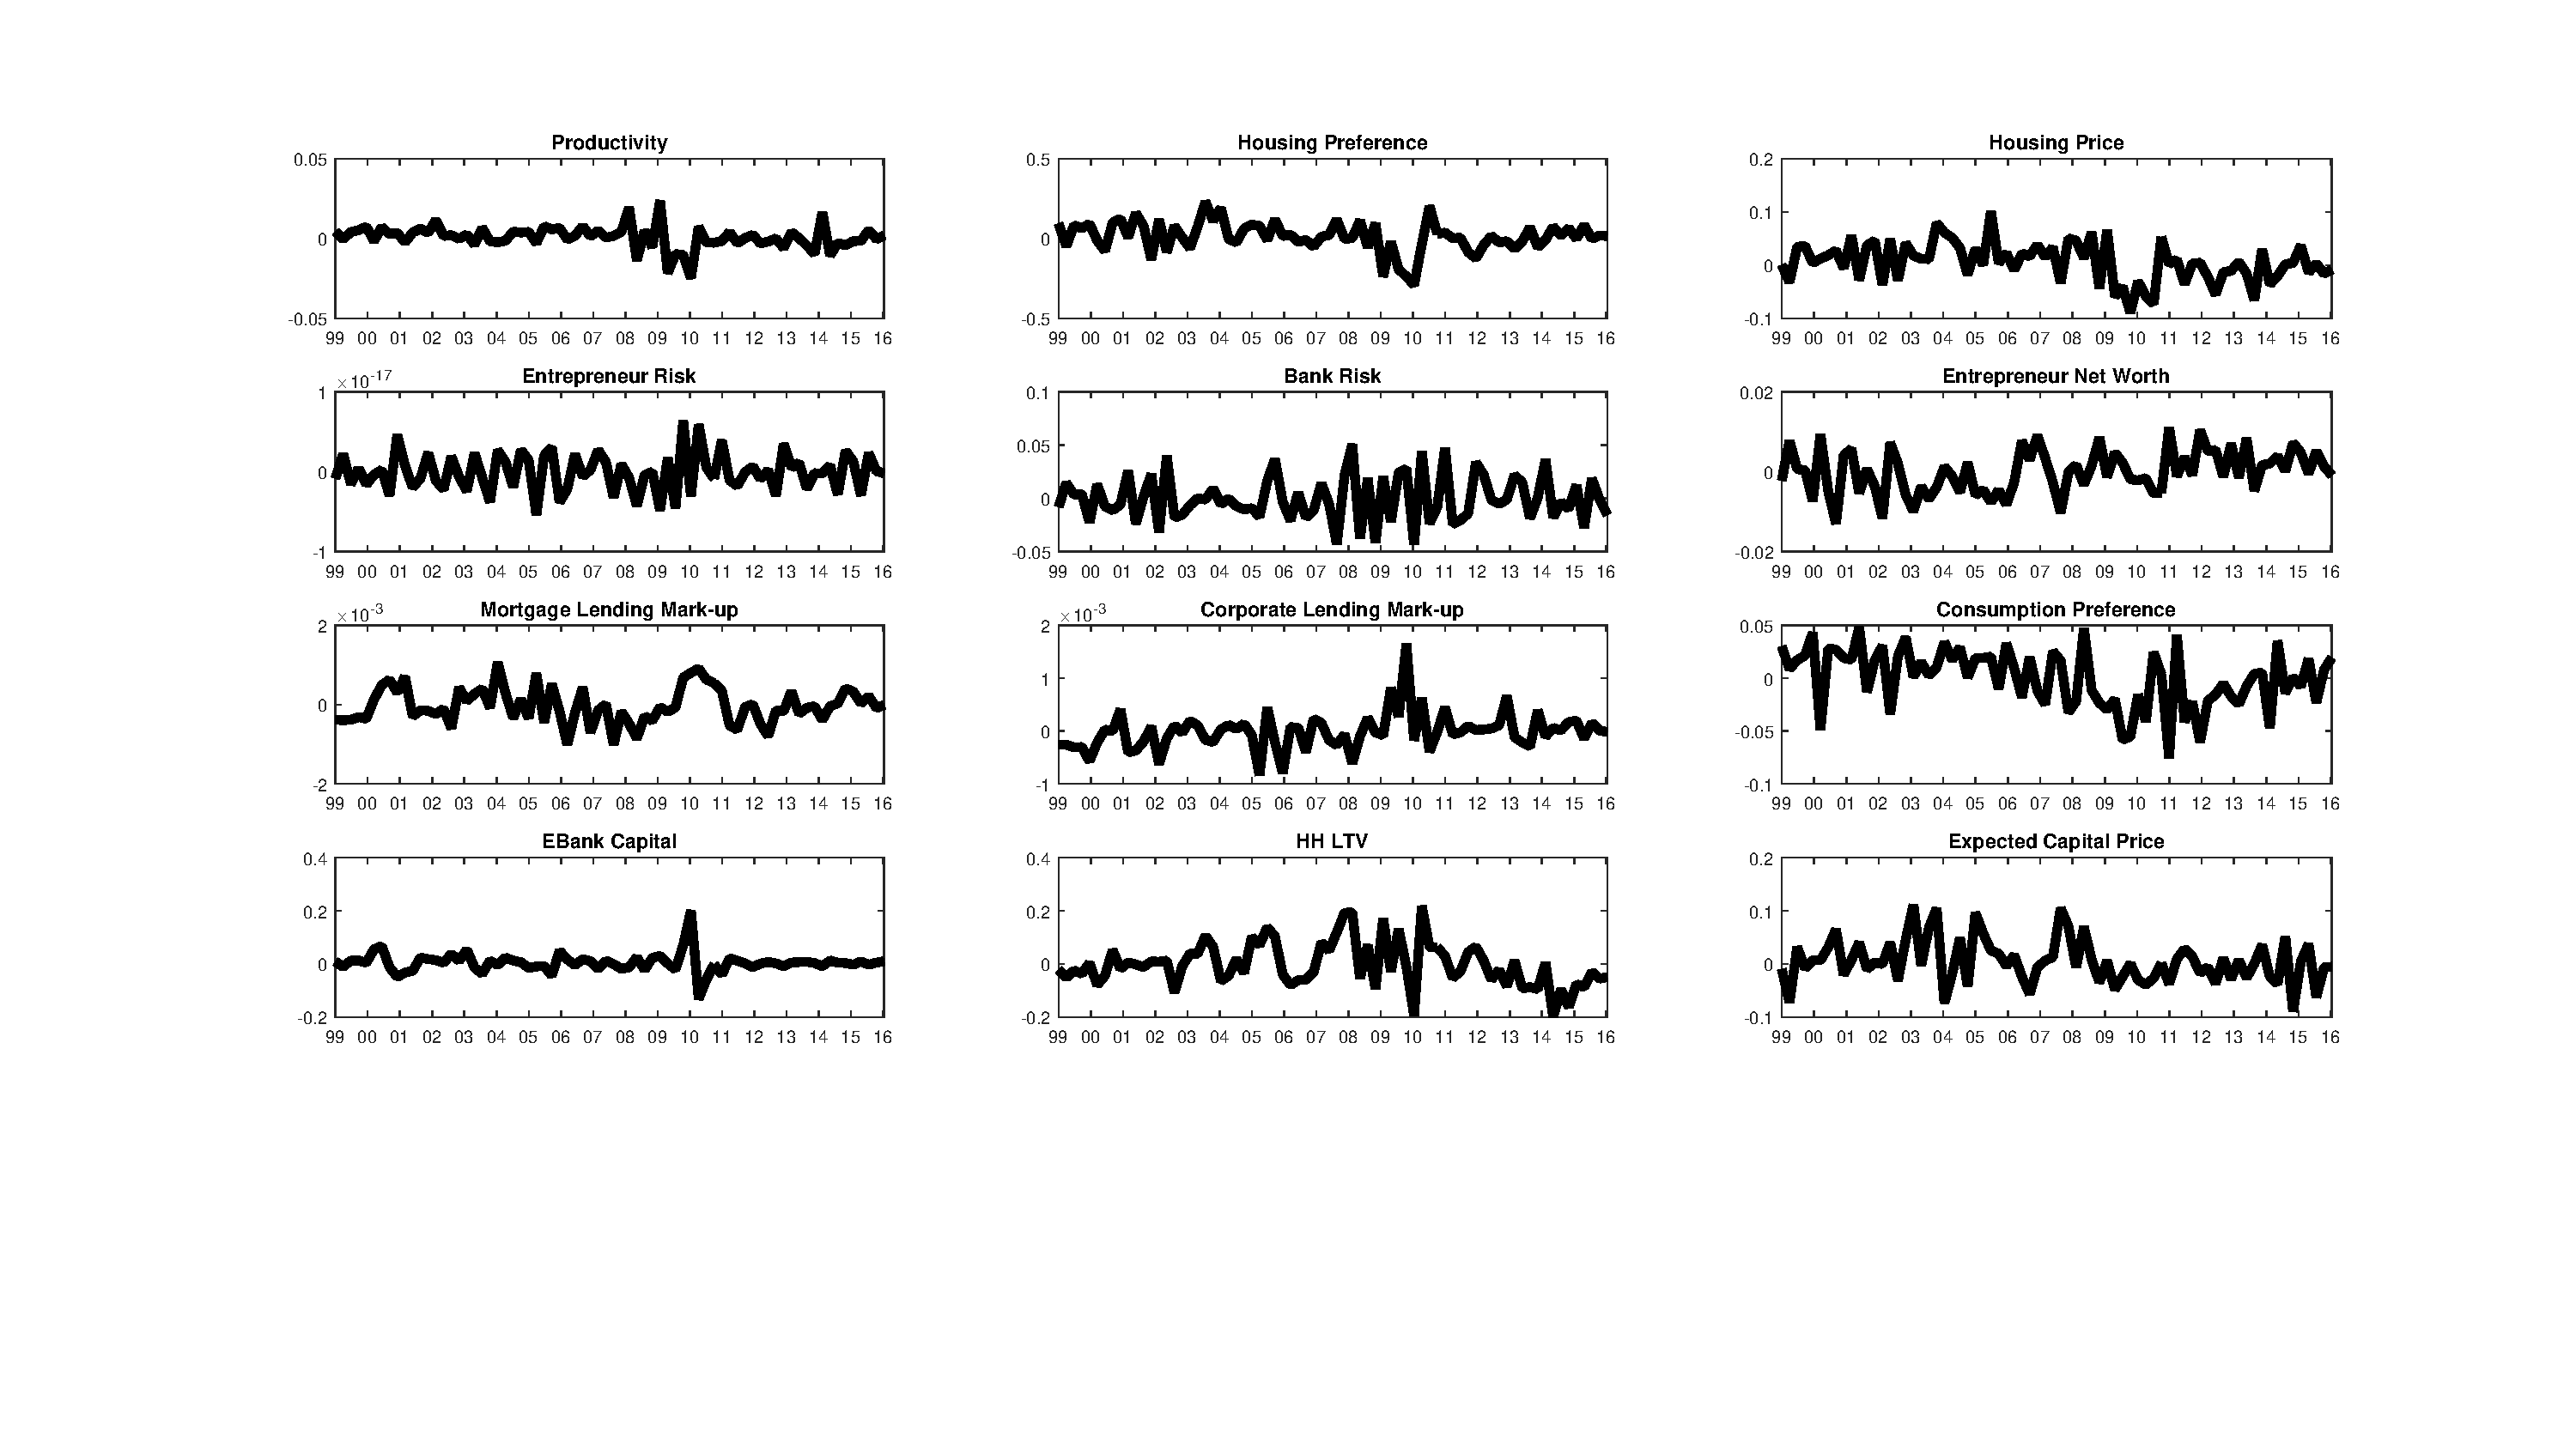
\includegraphics[scale=0.5]{smoothed_shocks.pdf}
\subfigure[Key shocks driving the financial crisis in the model.]{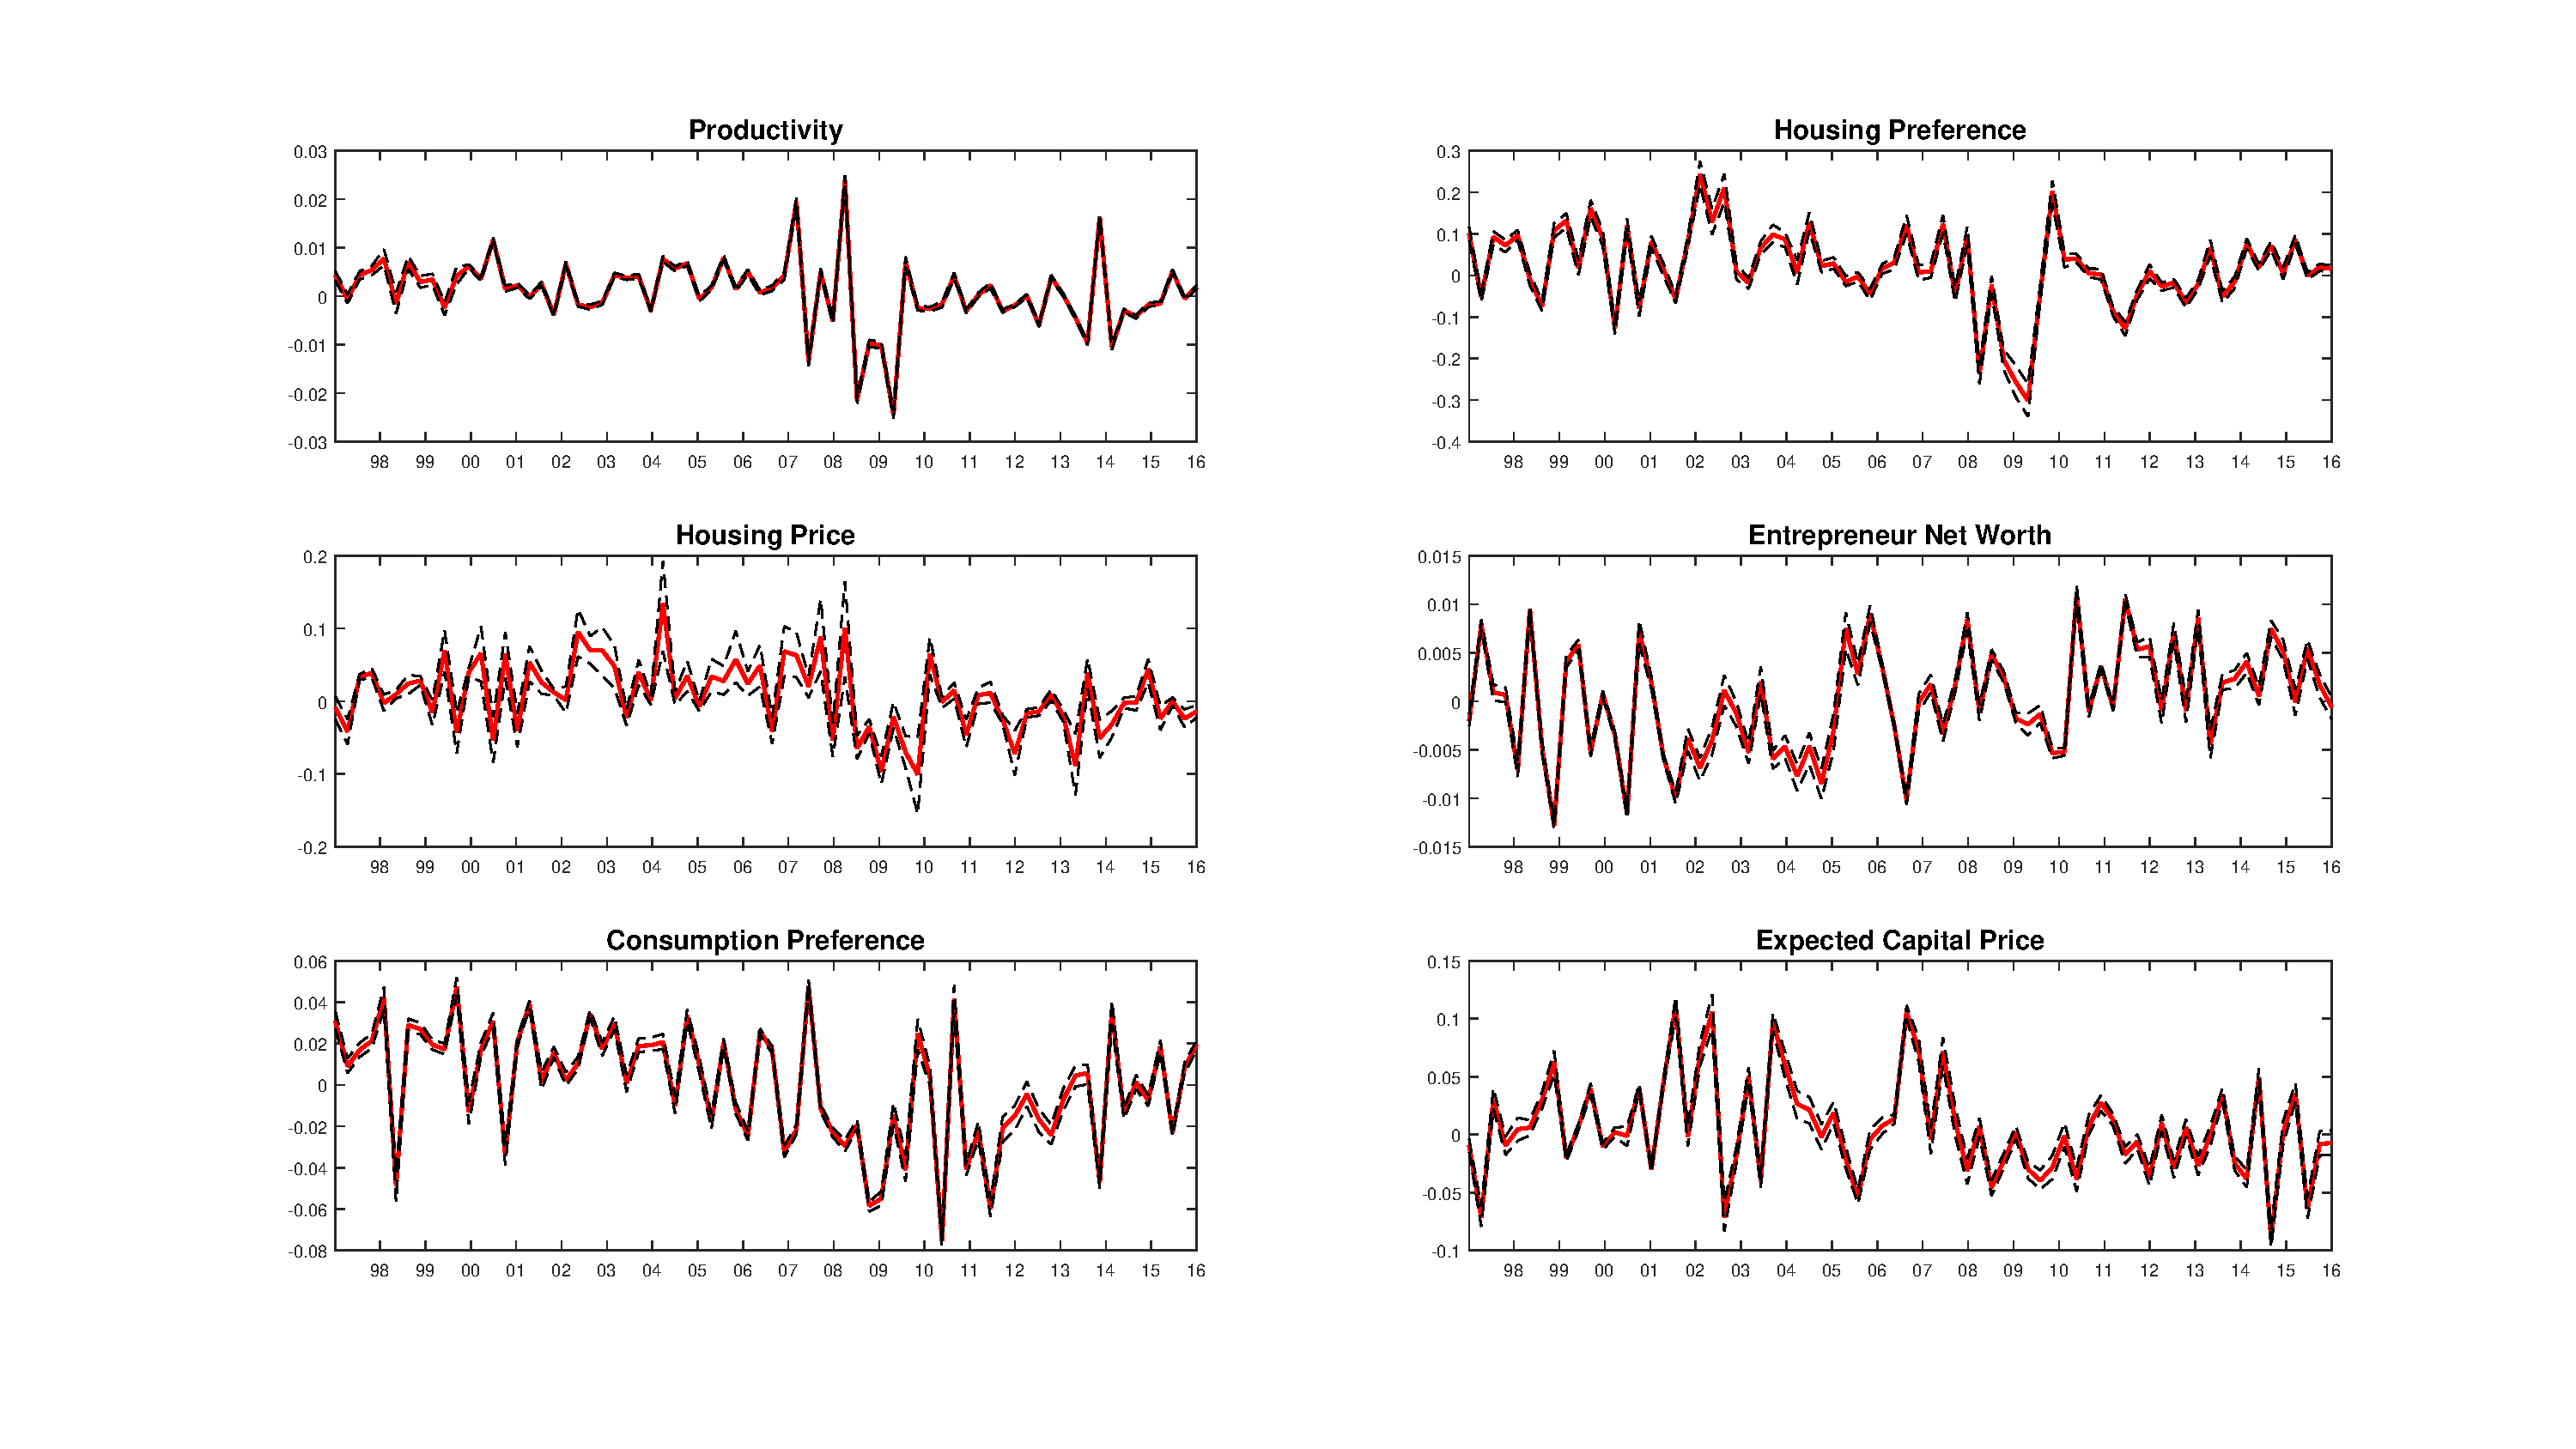
\includegraphics[scale=0.4]{smoothed_shocks_HPD.pdf}}\\
\subfigure[Default rates during the sample period, where y-axis shows the deviation in percentages from steady-state. ]{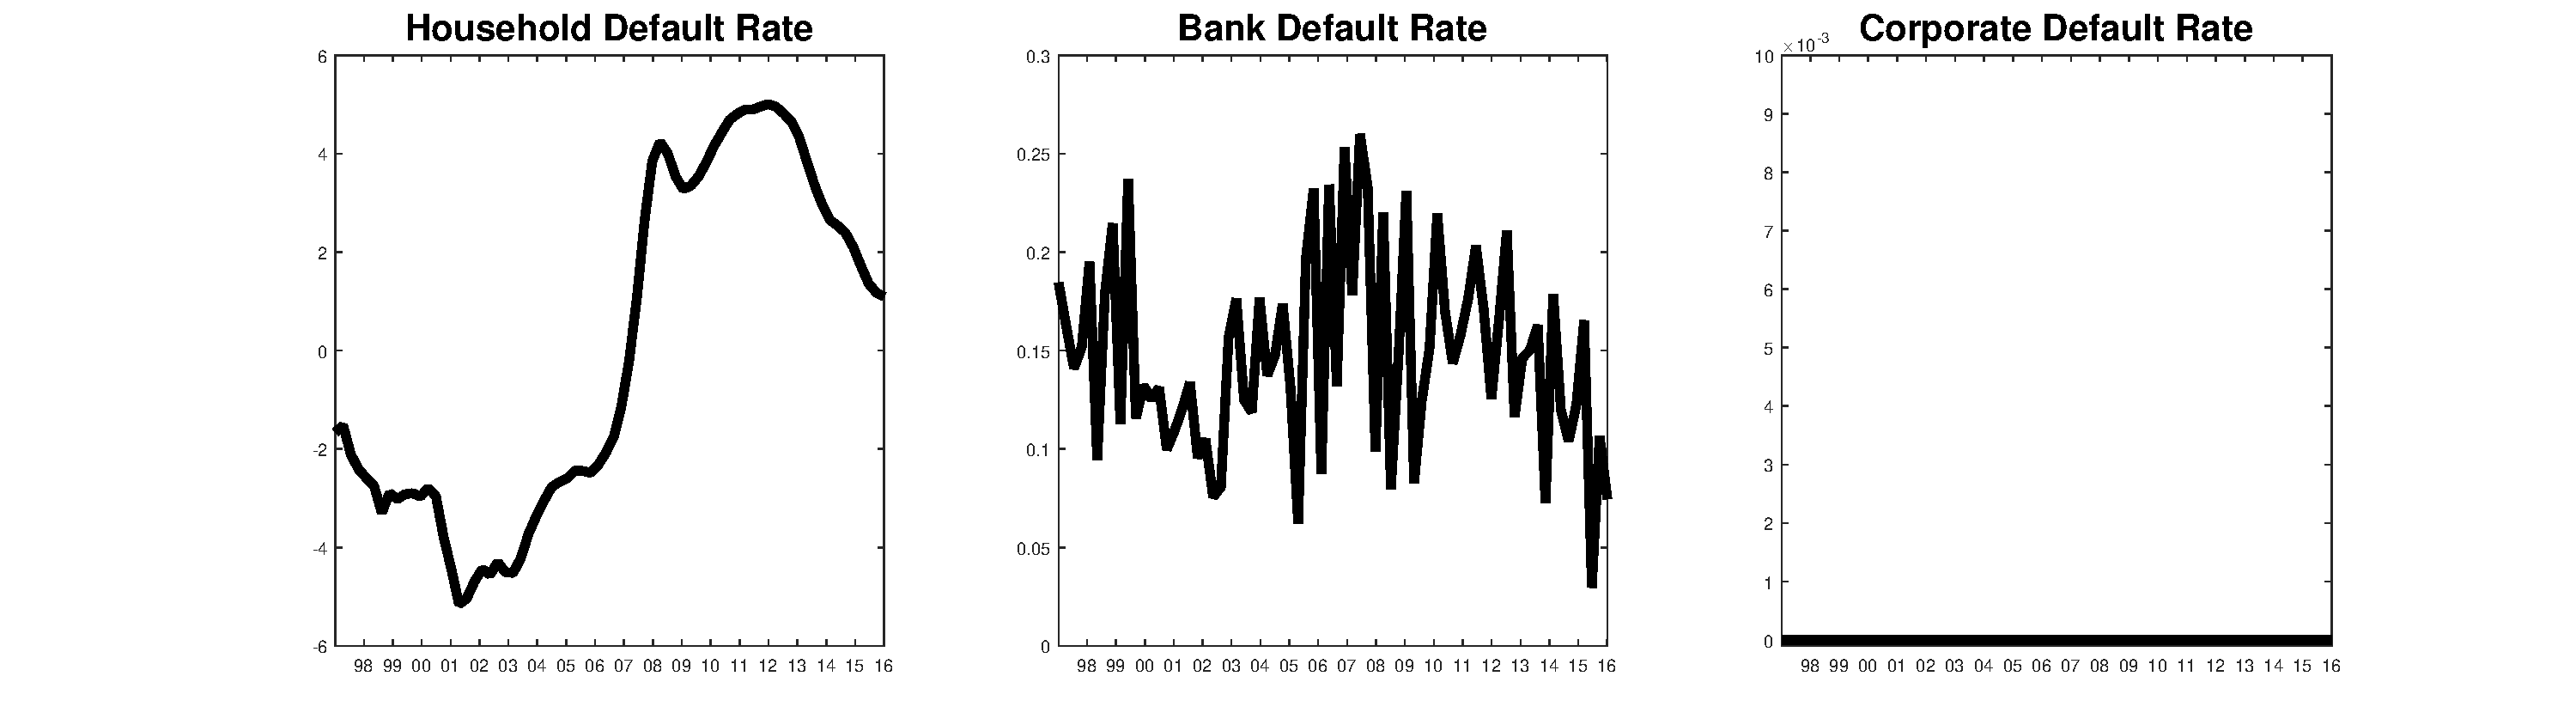
\includegraphics[scale=0.4]{smoothed_default_rates.pdf}}\\
\end{figure}


\FloatBarrier

\subsection{Variance Decompositions}

We next turn to variance decompositions of some key variables in order to see how the estimated shocks as discussed above transmit through the economy during the sample period. We focus on two variables in particular, namely the output growth and and mortgage lending growth rates, which are shown in Figure \ref{decomp_dbm} . The unconditional decompositions of some other observable variables is also reported in Table \ref{uncond_var_decomp}, which will be discussed further below. 

Starting with the mortgage lending growth rate, it is readily seen that the main drivers are housing preference and house price shocks as previously discussed. The external drop in house prices has a ceteris paribus effect of increasing housing demand and therefore demand for housing loans. Therefore the house price shocks contributes negatively to the mortgage lending growth during the pre-crisis period when house prices are increasing, and negatively during the post-crisis period when the housing price trend reverses. Given the house price shocks, the housing preference shocks are large enough to generate a positive growth before the crisis, and negative growth after the crisis. Aside from these shocks, bank capital and consumption preference shocks also play an smaller but non-negligible role in terms of driving mortgage lending growth. 

Next looking at output growth, we observe that four shocks emerge as important drivers, namely the productivity, entrepreneur net worth and consumption preference shocks. The housing preference shock also plays a role to a smaller extent, and the house price shock becomes particularly important with the onset of the crisis.  During the crisis period, all four of these shocks contribute negatively to output growth, whereas bank capital and house price shocks contribute positively. Interestingly, the productivity shock contributes positively throughout the early 2000s until the crisis, while it contributes negatively for a long period after the crisis until mid-2015. The contributions from consumption preference turn positive shortly after the crisis, while the negative ones from housing preference persists. The entrepreneur net worth shock, while playing a relatively large role overall, has periods of both positive and negative contributions both before and after the crisis. Accordingly, the low output growth rate post-crisis is explained by productivity and housing preference shocks, and to some extent the entrepreneur net worth shocks. The positive contribution from house price shocks during the crisis period works through the channel of boosting housing demand and investment. Therefore we interpret this shock on output growth as picking up the effects of a looser monetary policy, which would work through the same channel of boosting demand and investment. 


Table \ref{uncond_var_decomp} shows the unconditional decompositions of output and mortgage lending growth rates, along with the other growth rates used as observables in the estimation. It is readily seen that, as discussed above, the output growth rate is mainly dominated by productivity, consumption preference and entrepreneur net worth shocks. The role for both housing shocks are substantially reduced compared to historical decomposition, which is intuitive since these shocks affect output growth mostly during the period surrounding the crisis. Similarly, the housing preference and housing price shocks are the dominant drivers both for house price and mortgage lending growth rates\footnote{For lending growth rates, bank capital shock also plays an important role, making up around 25 \% of the fluctuations for both variables. Hence the contribution from the \textit{other shocks} category mainly consists of the bank capital shock for these variables, while the \textit{other shocks} category does not play a substantial role for the other variables.}

For corporate lending growth rate, the expected capital price and entrepreneur net worth shocks are the dominant players as expected, while wage growth rate is mainly driven by productivity shocks. Finally, consumption growth rate is mainly dominated by productivity and consumption preference shocks, which is similar to output growth rate with the exception that the role of entrepreneur net worth shock is absorbed by preference shocks.


%\begin{figure}[H]
%\centering
%\caption{Official Bank Rate}
%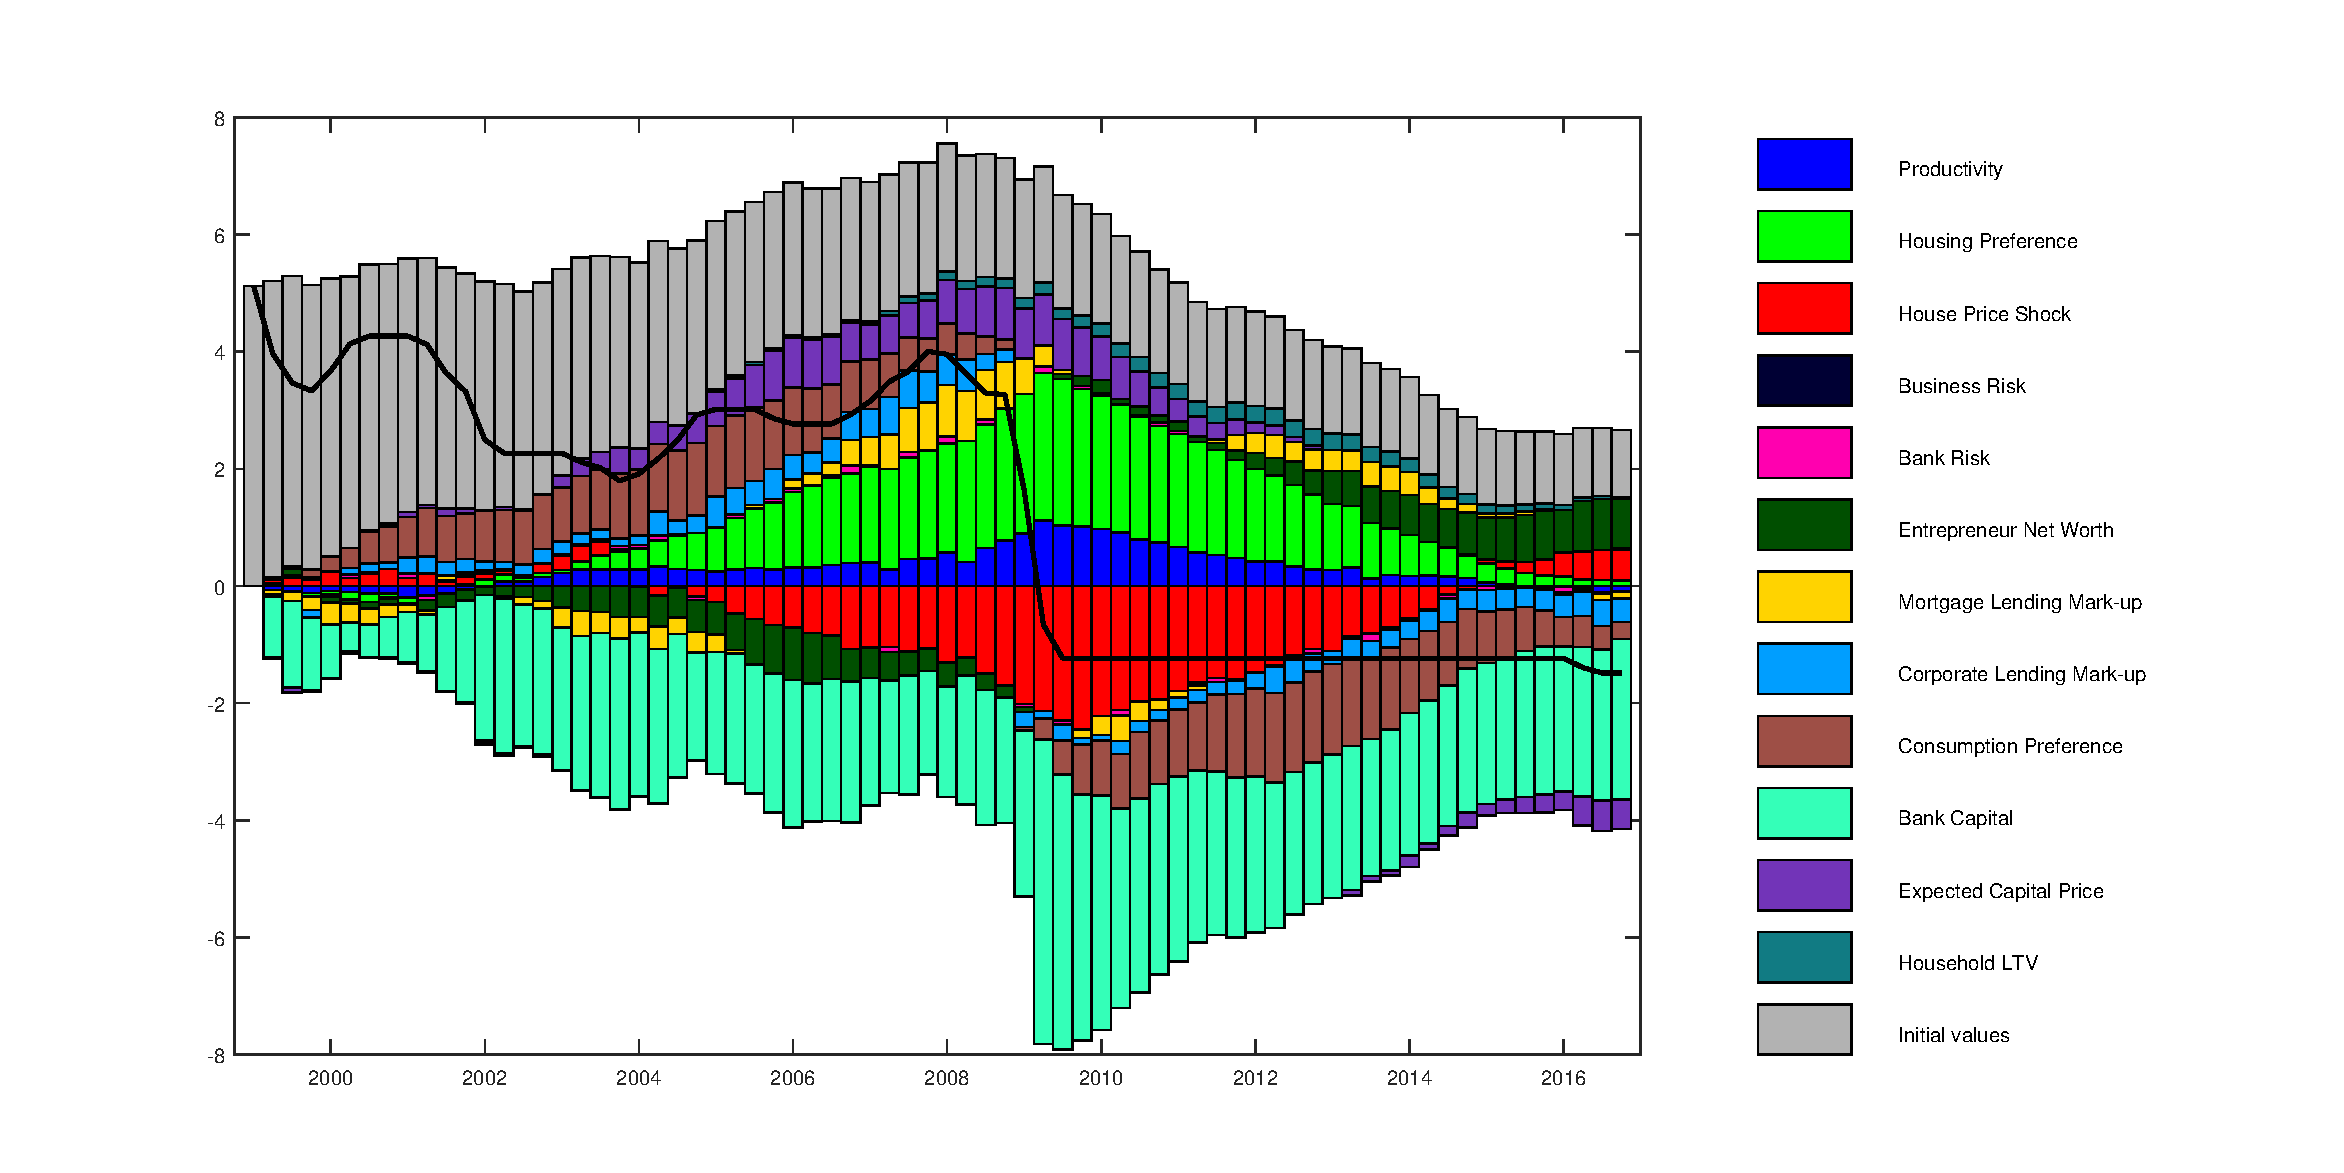
\includegraphics[scale=0.45]{decomp_bank_rate.pdf}
%\end{figure}


%\begin{figure}[H]
%\centering
%\caption{Mortgage Lending Rate}
%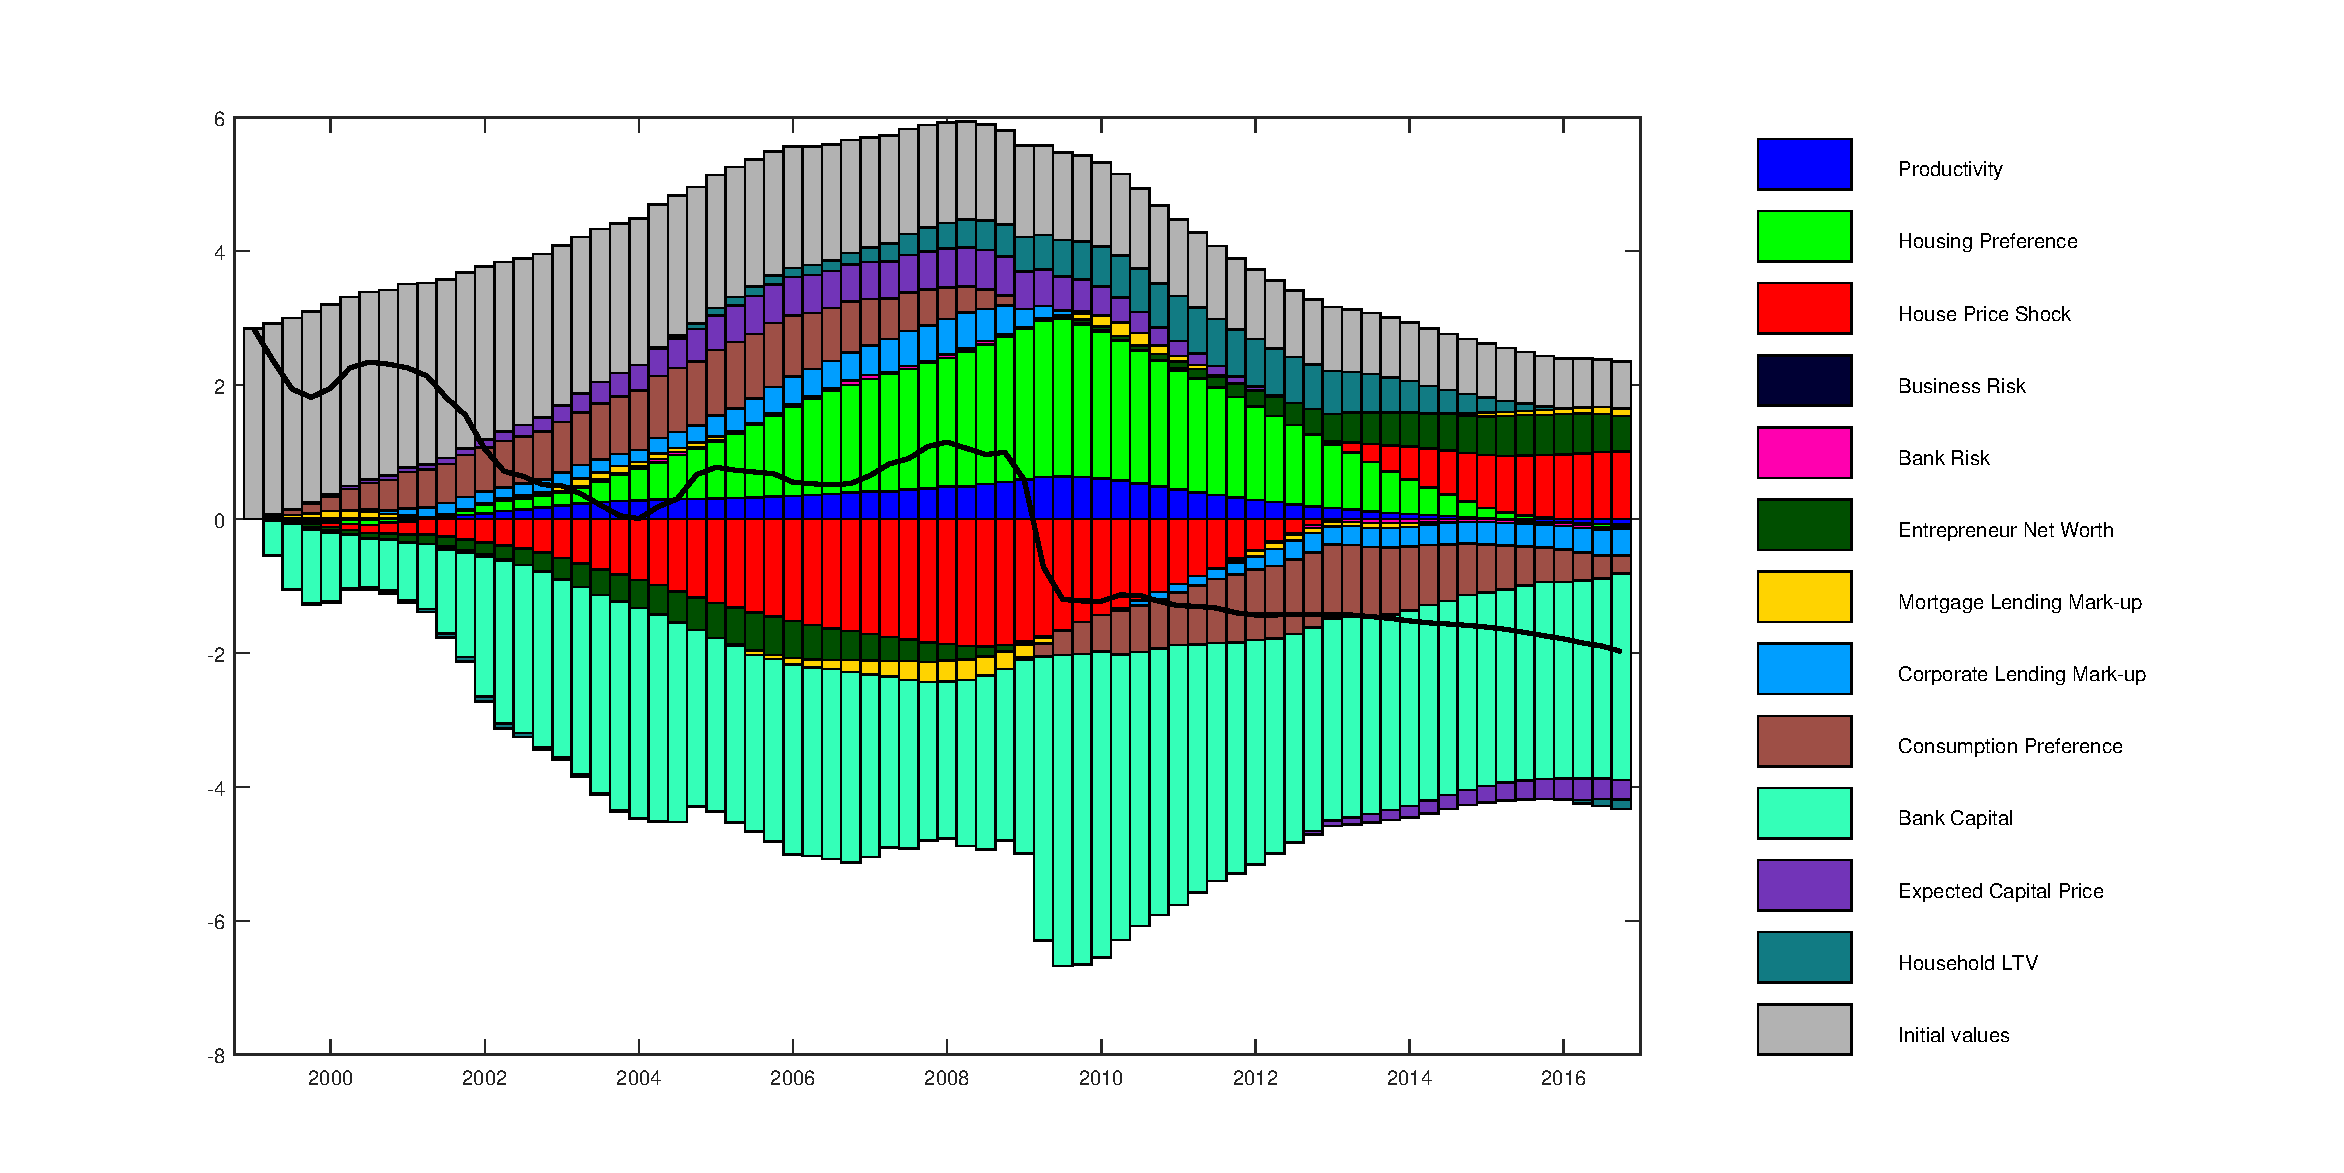
\includegraphics[scale=0.45]{decomp_int_rate_HH.pdf}
%\end{figure}

%\begin{figure}[H]
%\centering
%\caption{Corporate Lending Rate}
%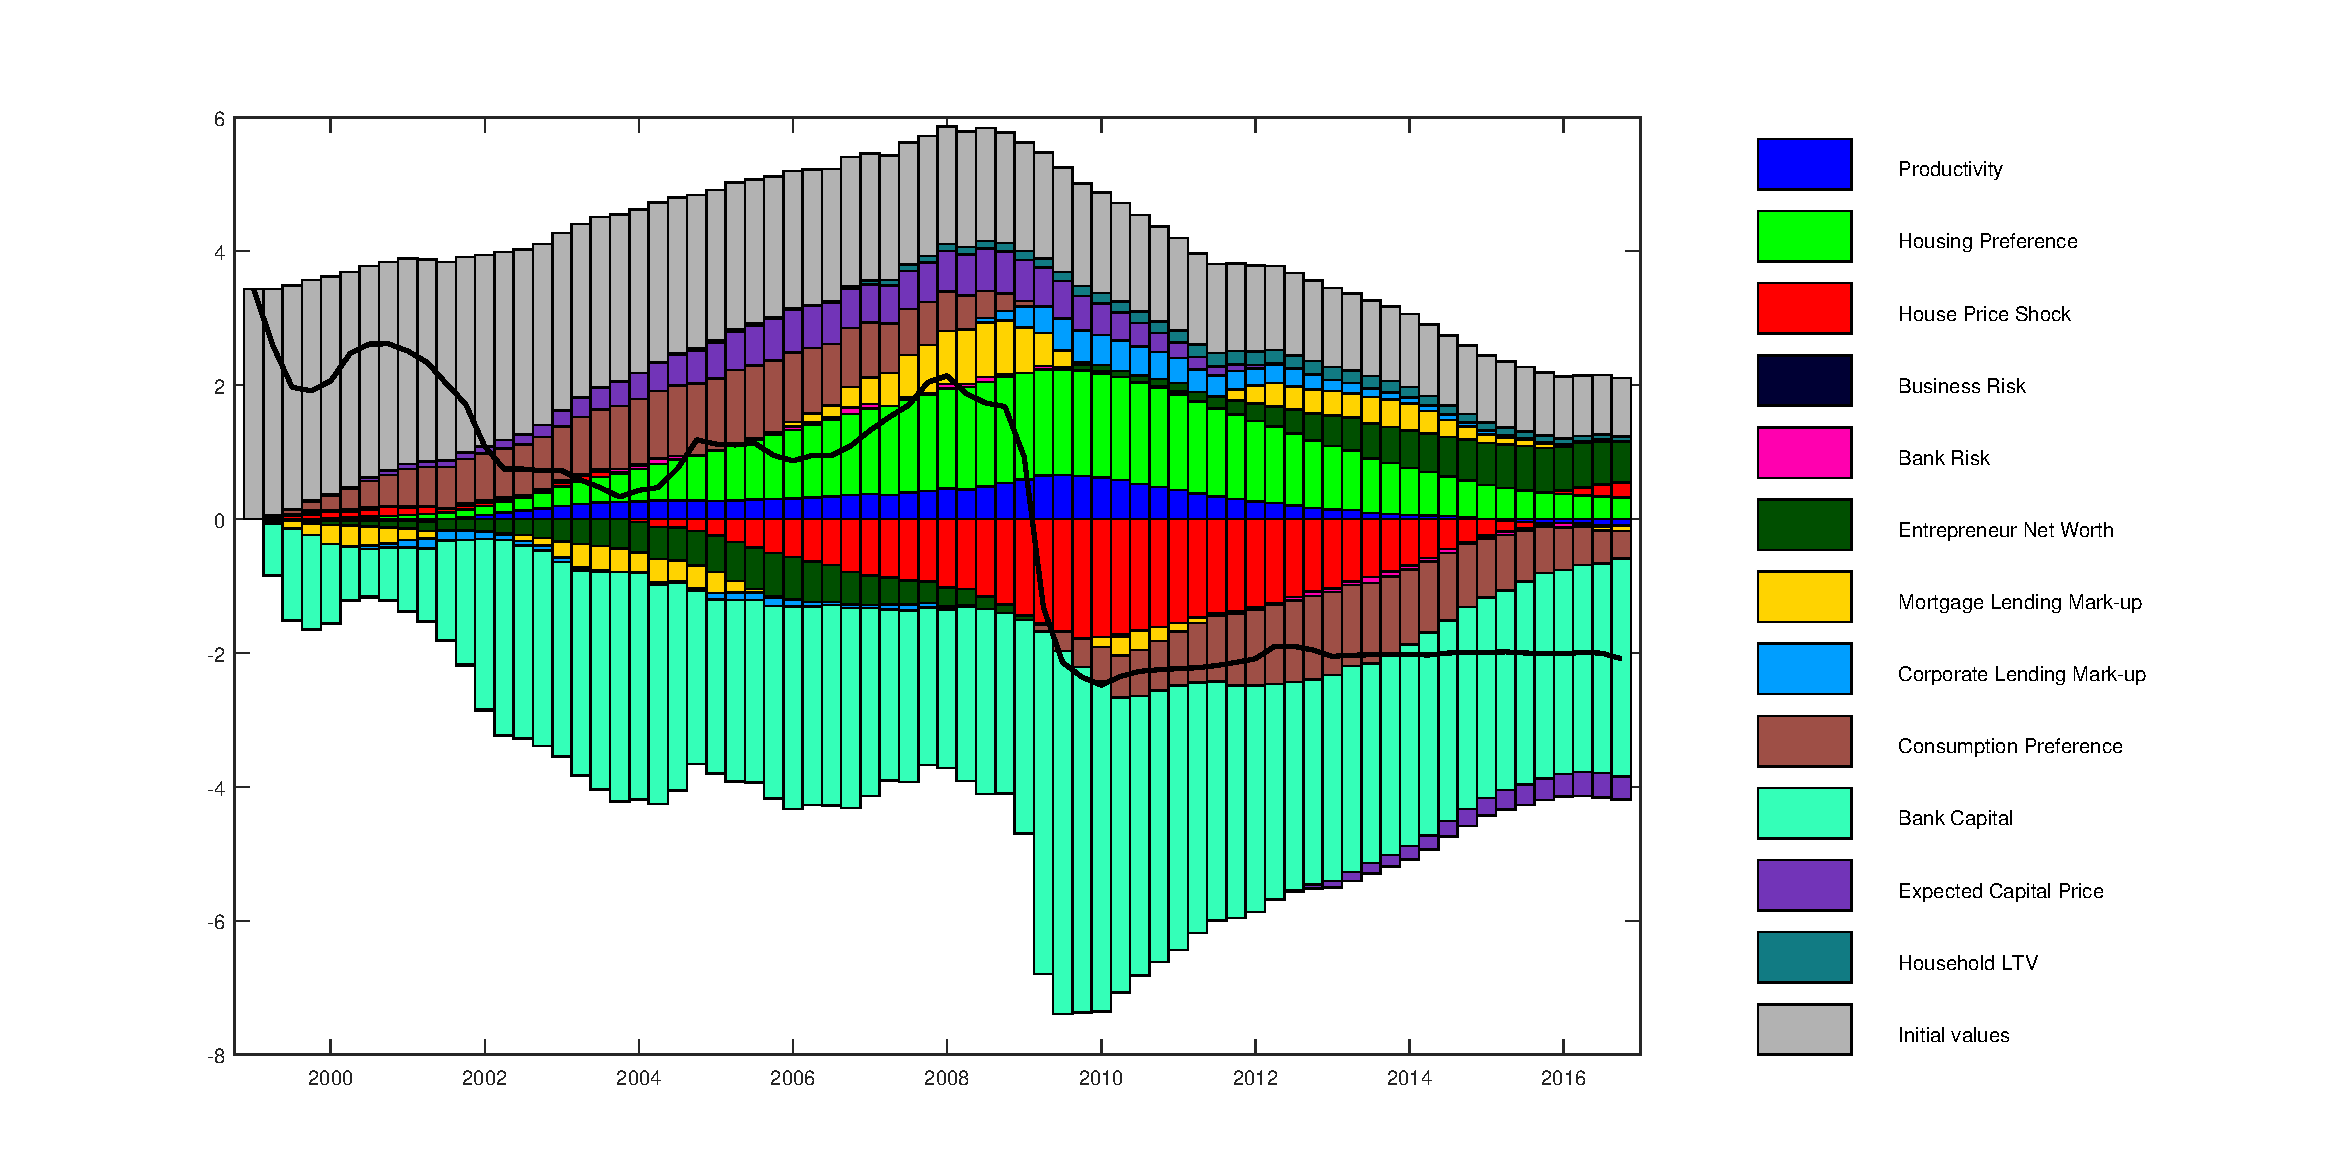
\includegraphics[scale=0.45]{decomp_int_rate_business.pdf}
%\end{figure}



%\begin{figure}[H]
%\centering
%\caption{Growth of Business Lending}
%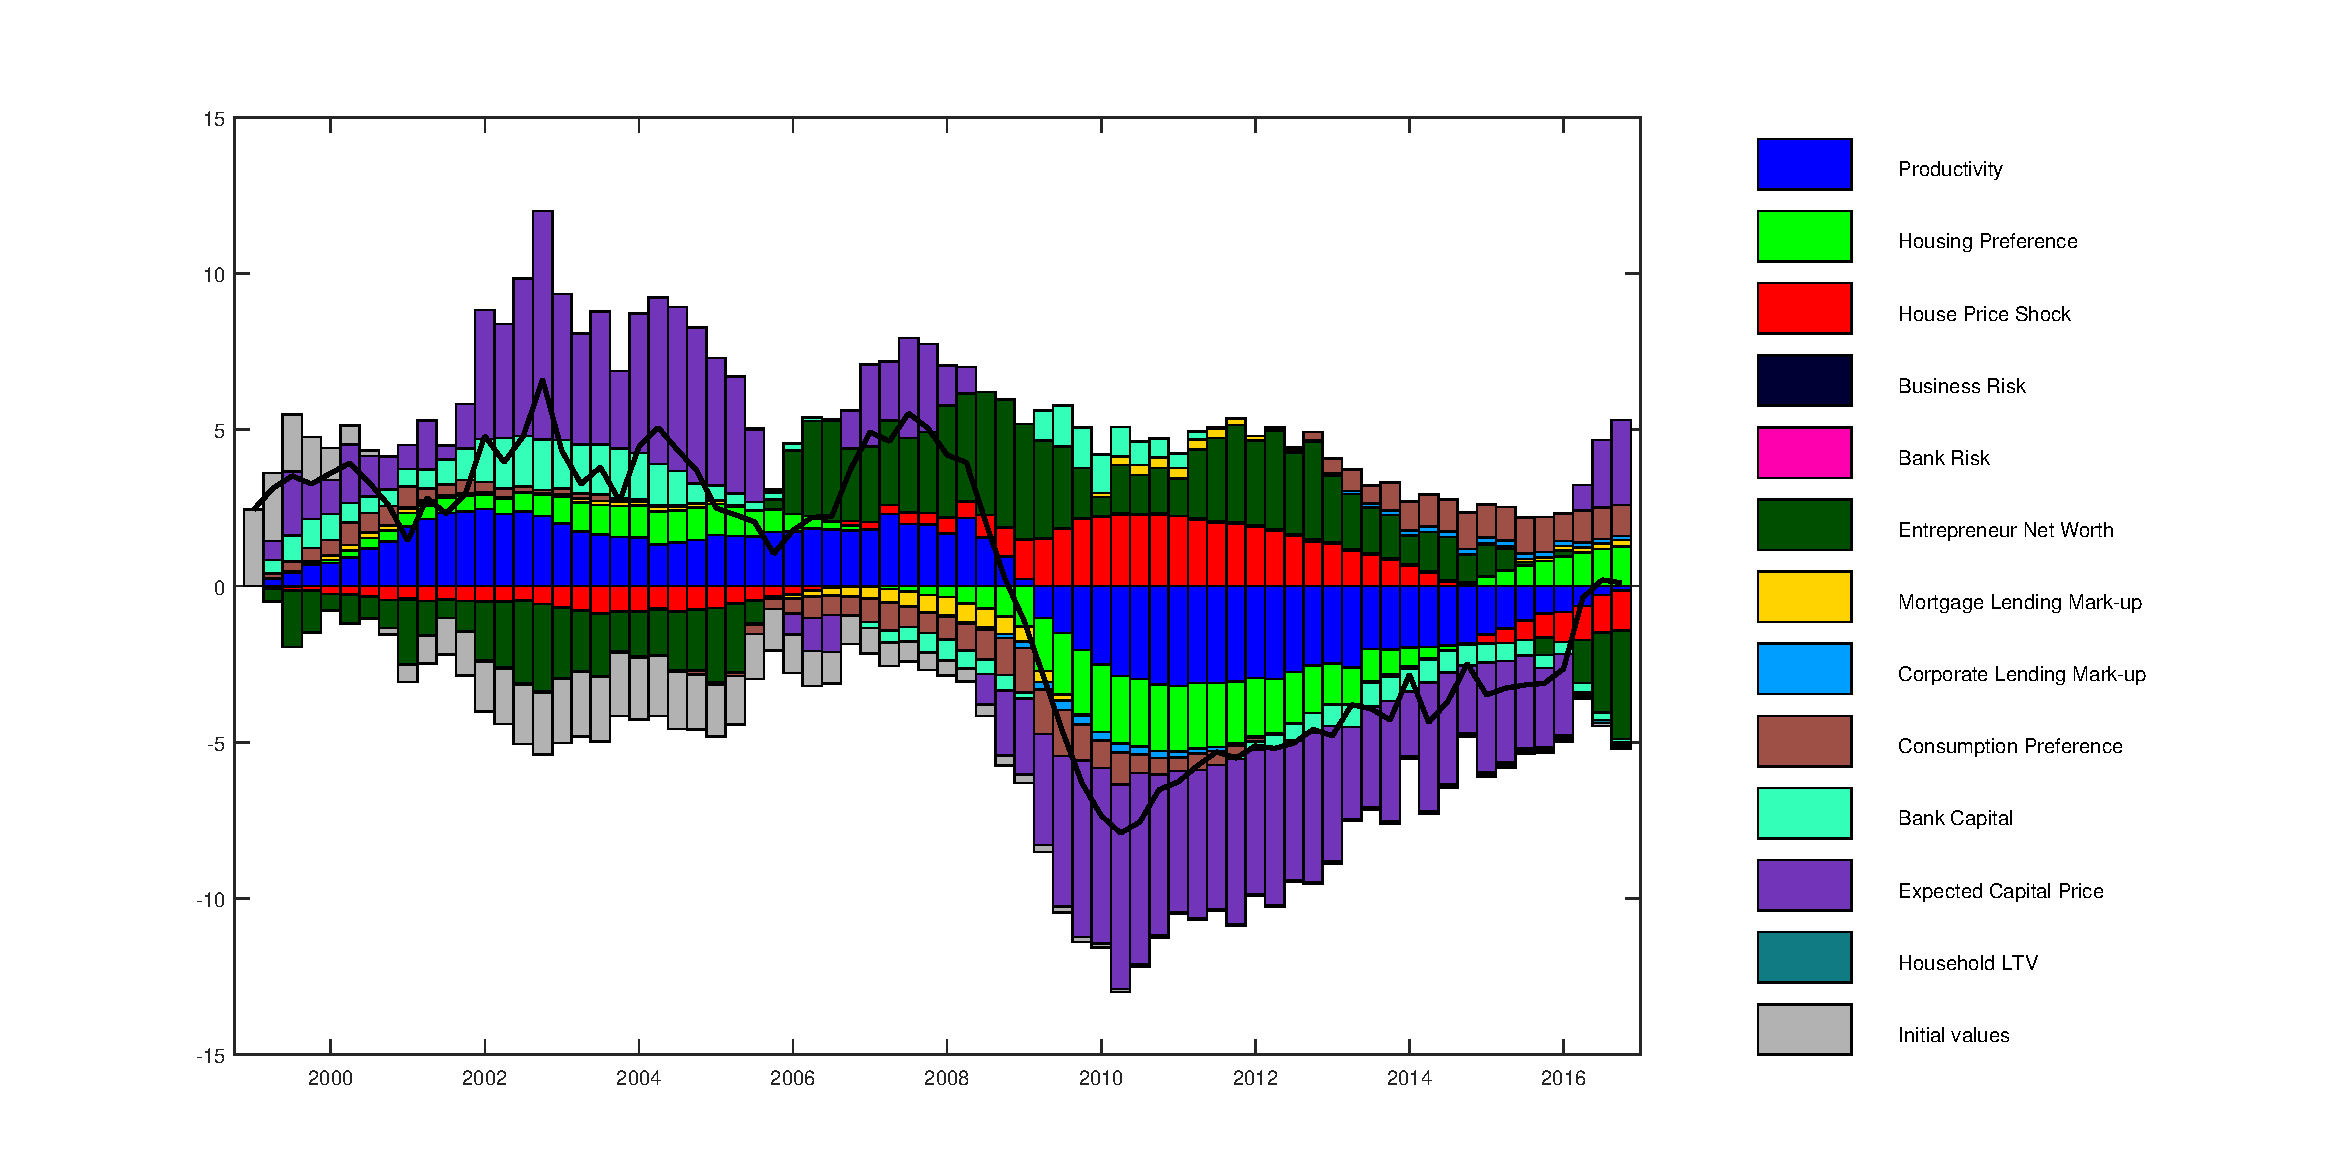
\includegraphics[scale=0.45]{decomp_dbe.pdf}
%\end{figure}


\begin{figure}[H]
\centering
\caption{Historical variance decompositions of mortgage lending and output growth rates.}
\label{decomp_dbm}
\subfigure[Mortgage lending growth rate.]{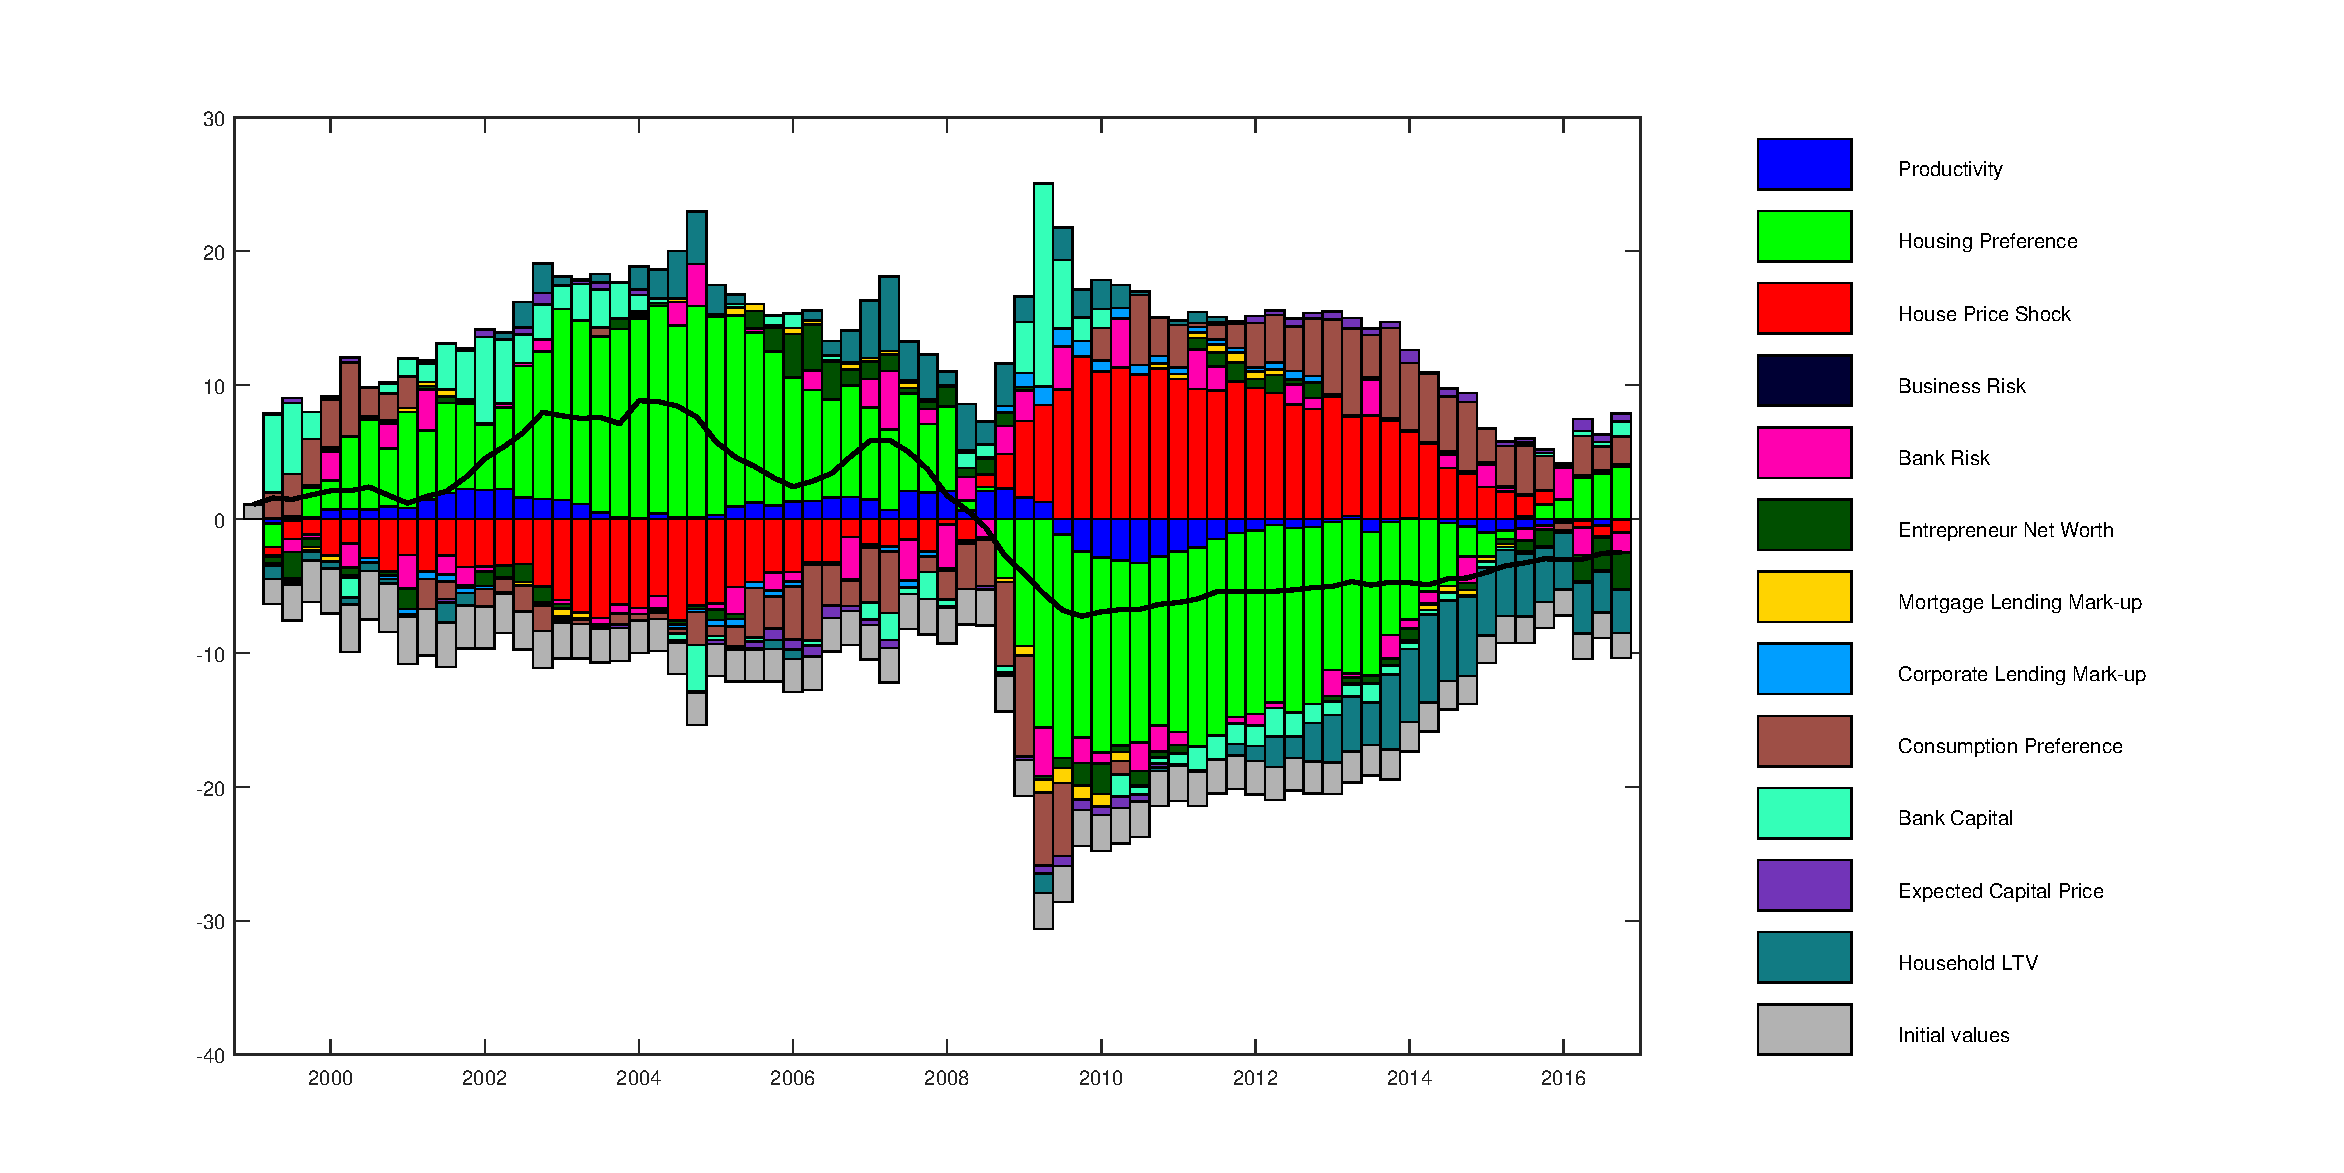
\includegraphics[scale=0.45]{decomp_dbm.pdf}}
\subfigure[Output growth rate.]{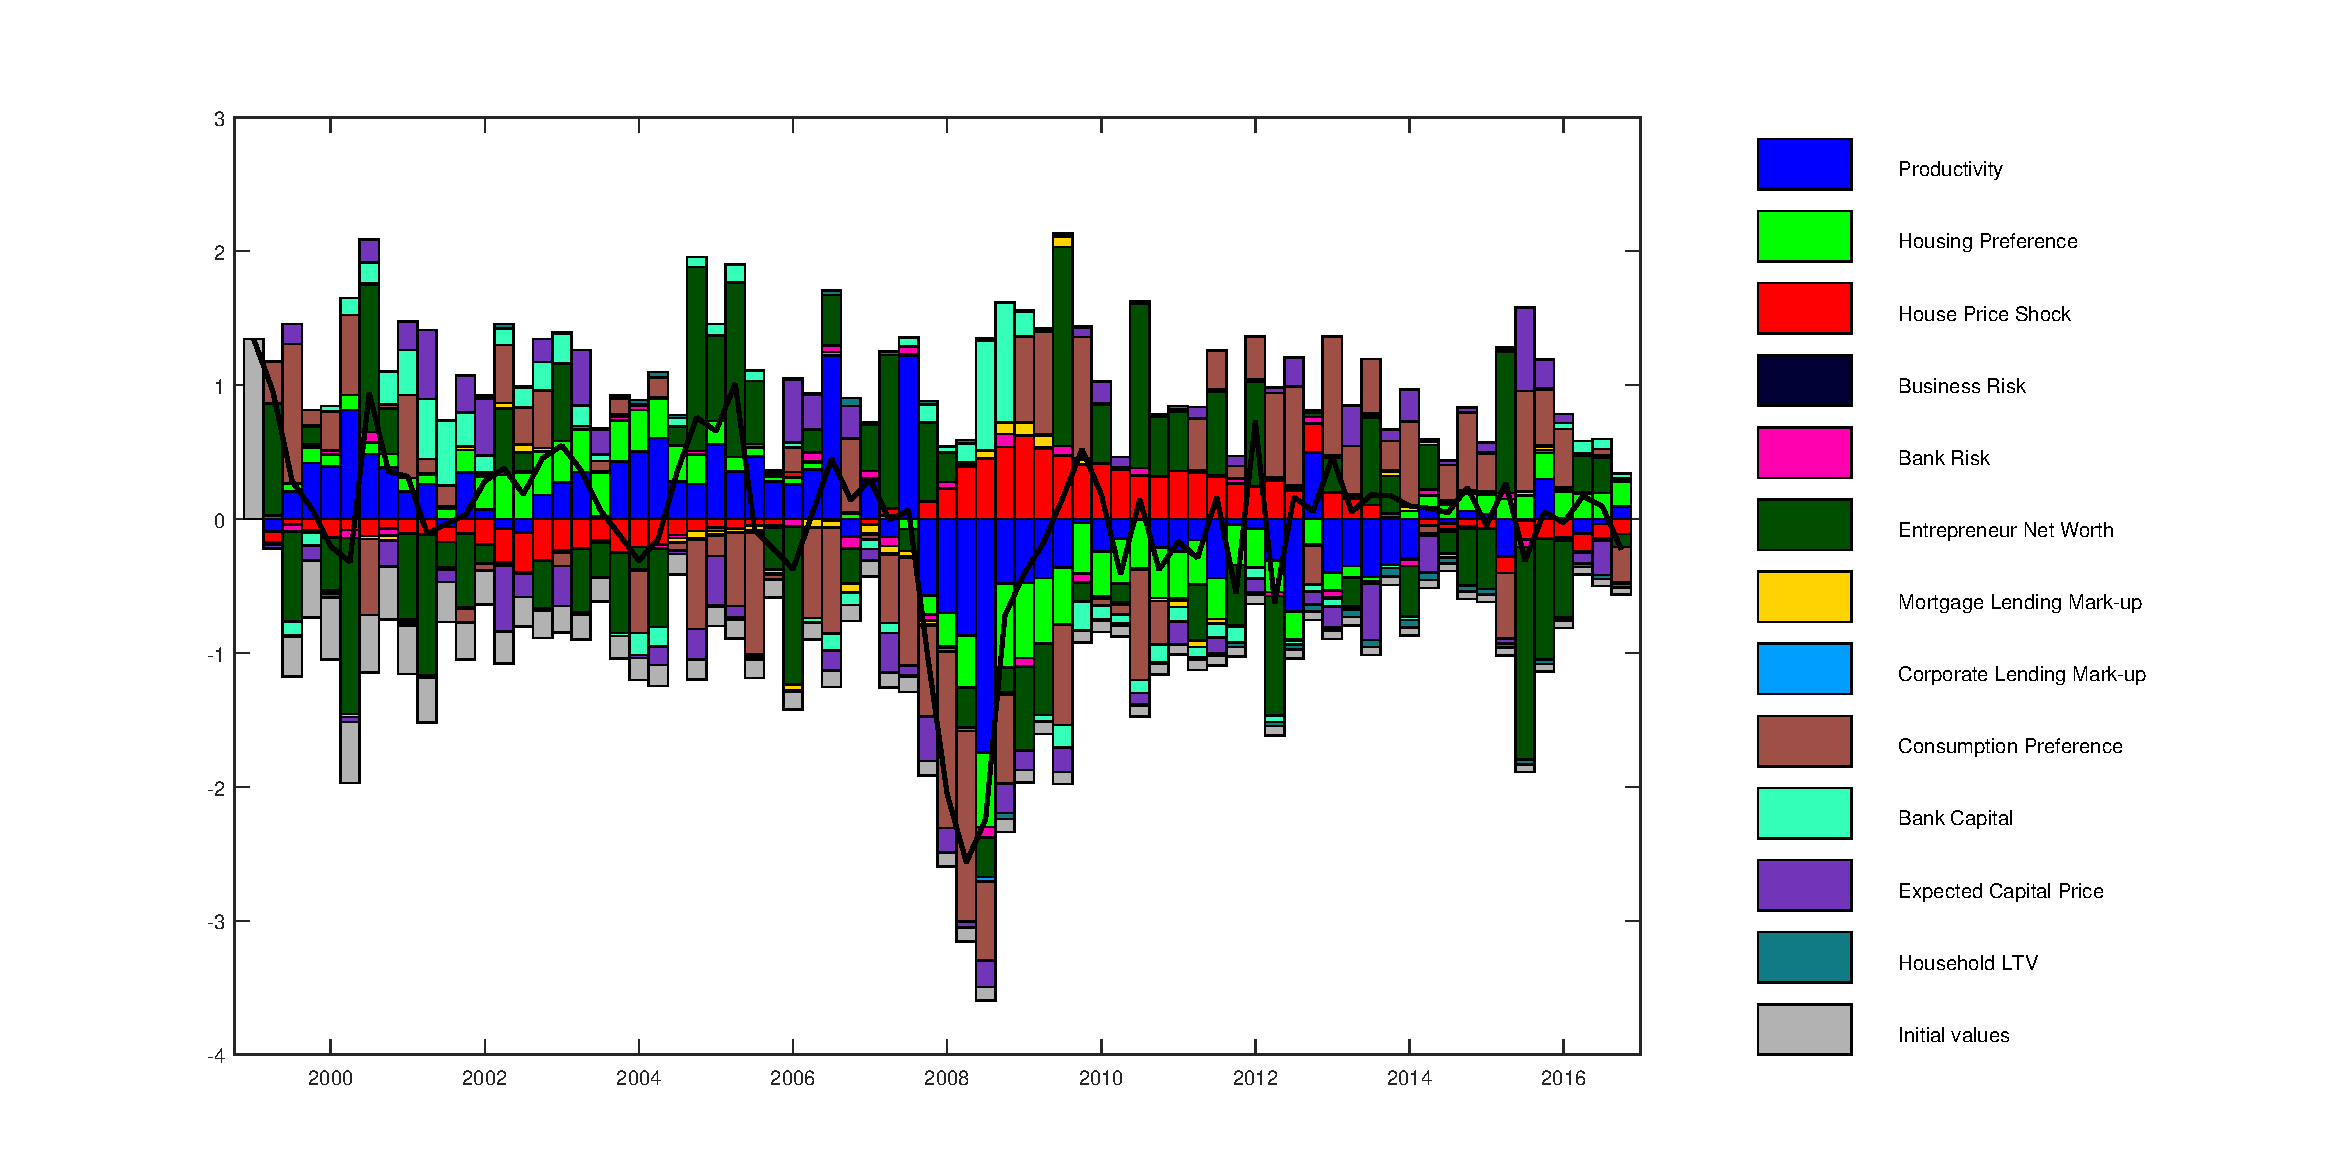
\includegraphics[scale=0.45]{decomp_dy.pdf}}
\end{figure}


%\begin{figure}[H]
%\centering
%\caption{House Price Growth}
%\includegraphics[scale=0.45]{decomp_dqH.pdf}
%\end{figure}




%\begin{figure}[H]
%\centering
%\caption{Investment Growth}
%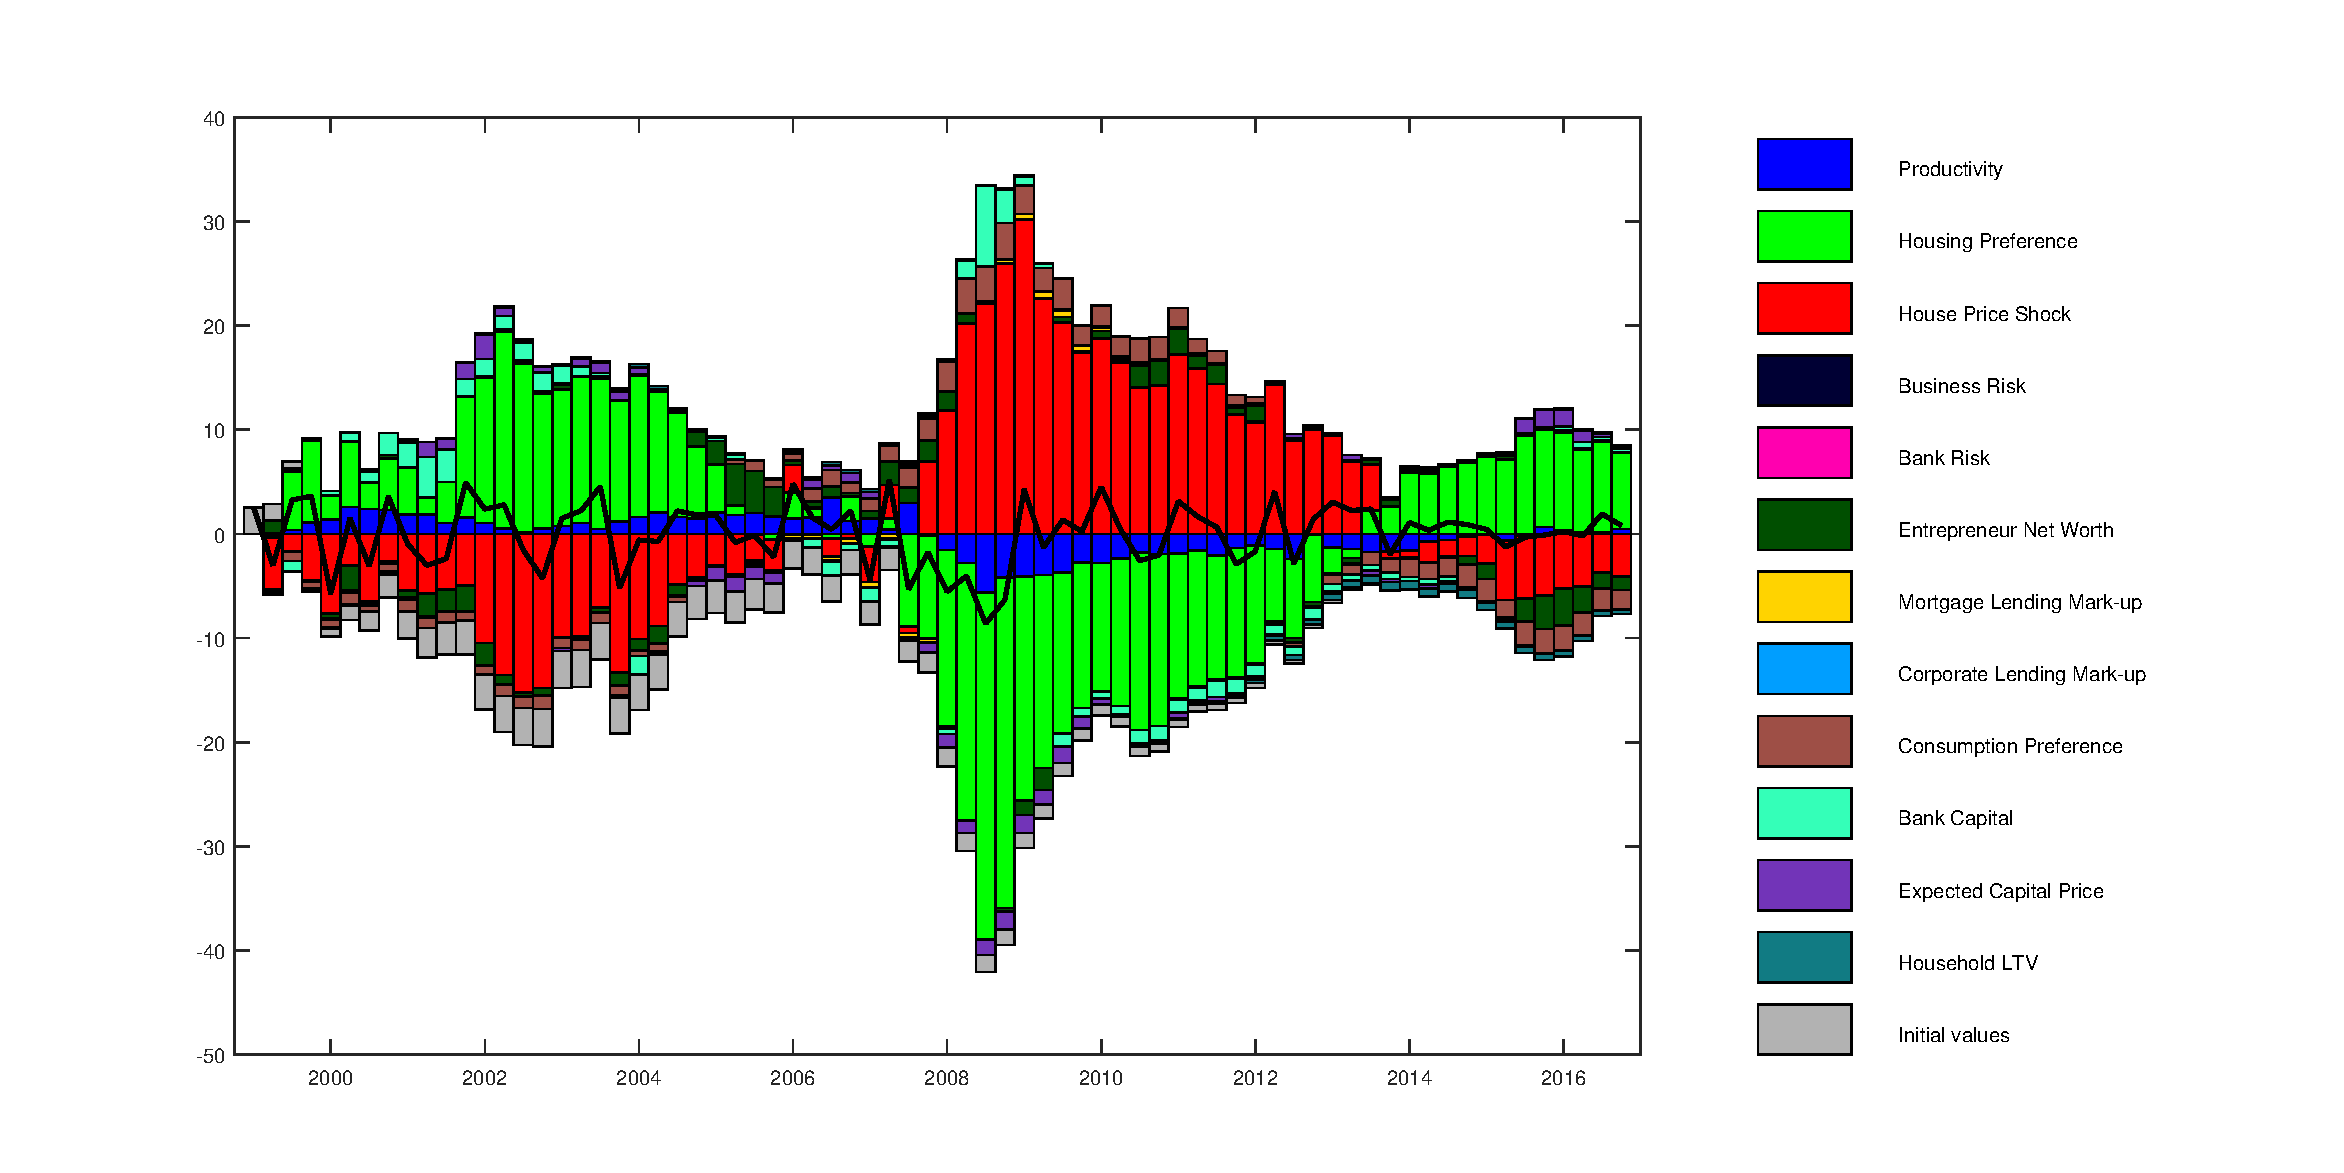
\includegraphics[scale=0.45]{decomp_dinve.pdf}
%\end{figure}



%\begin{figure}[H]
%\centering
%\caption{Consumption Growth}
%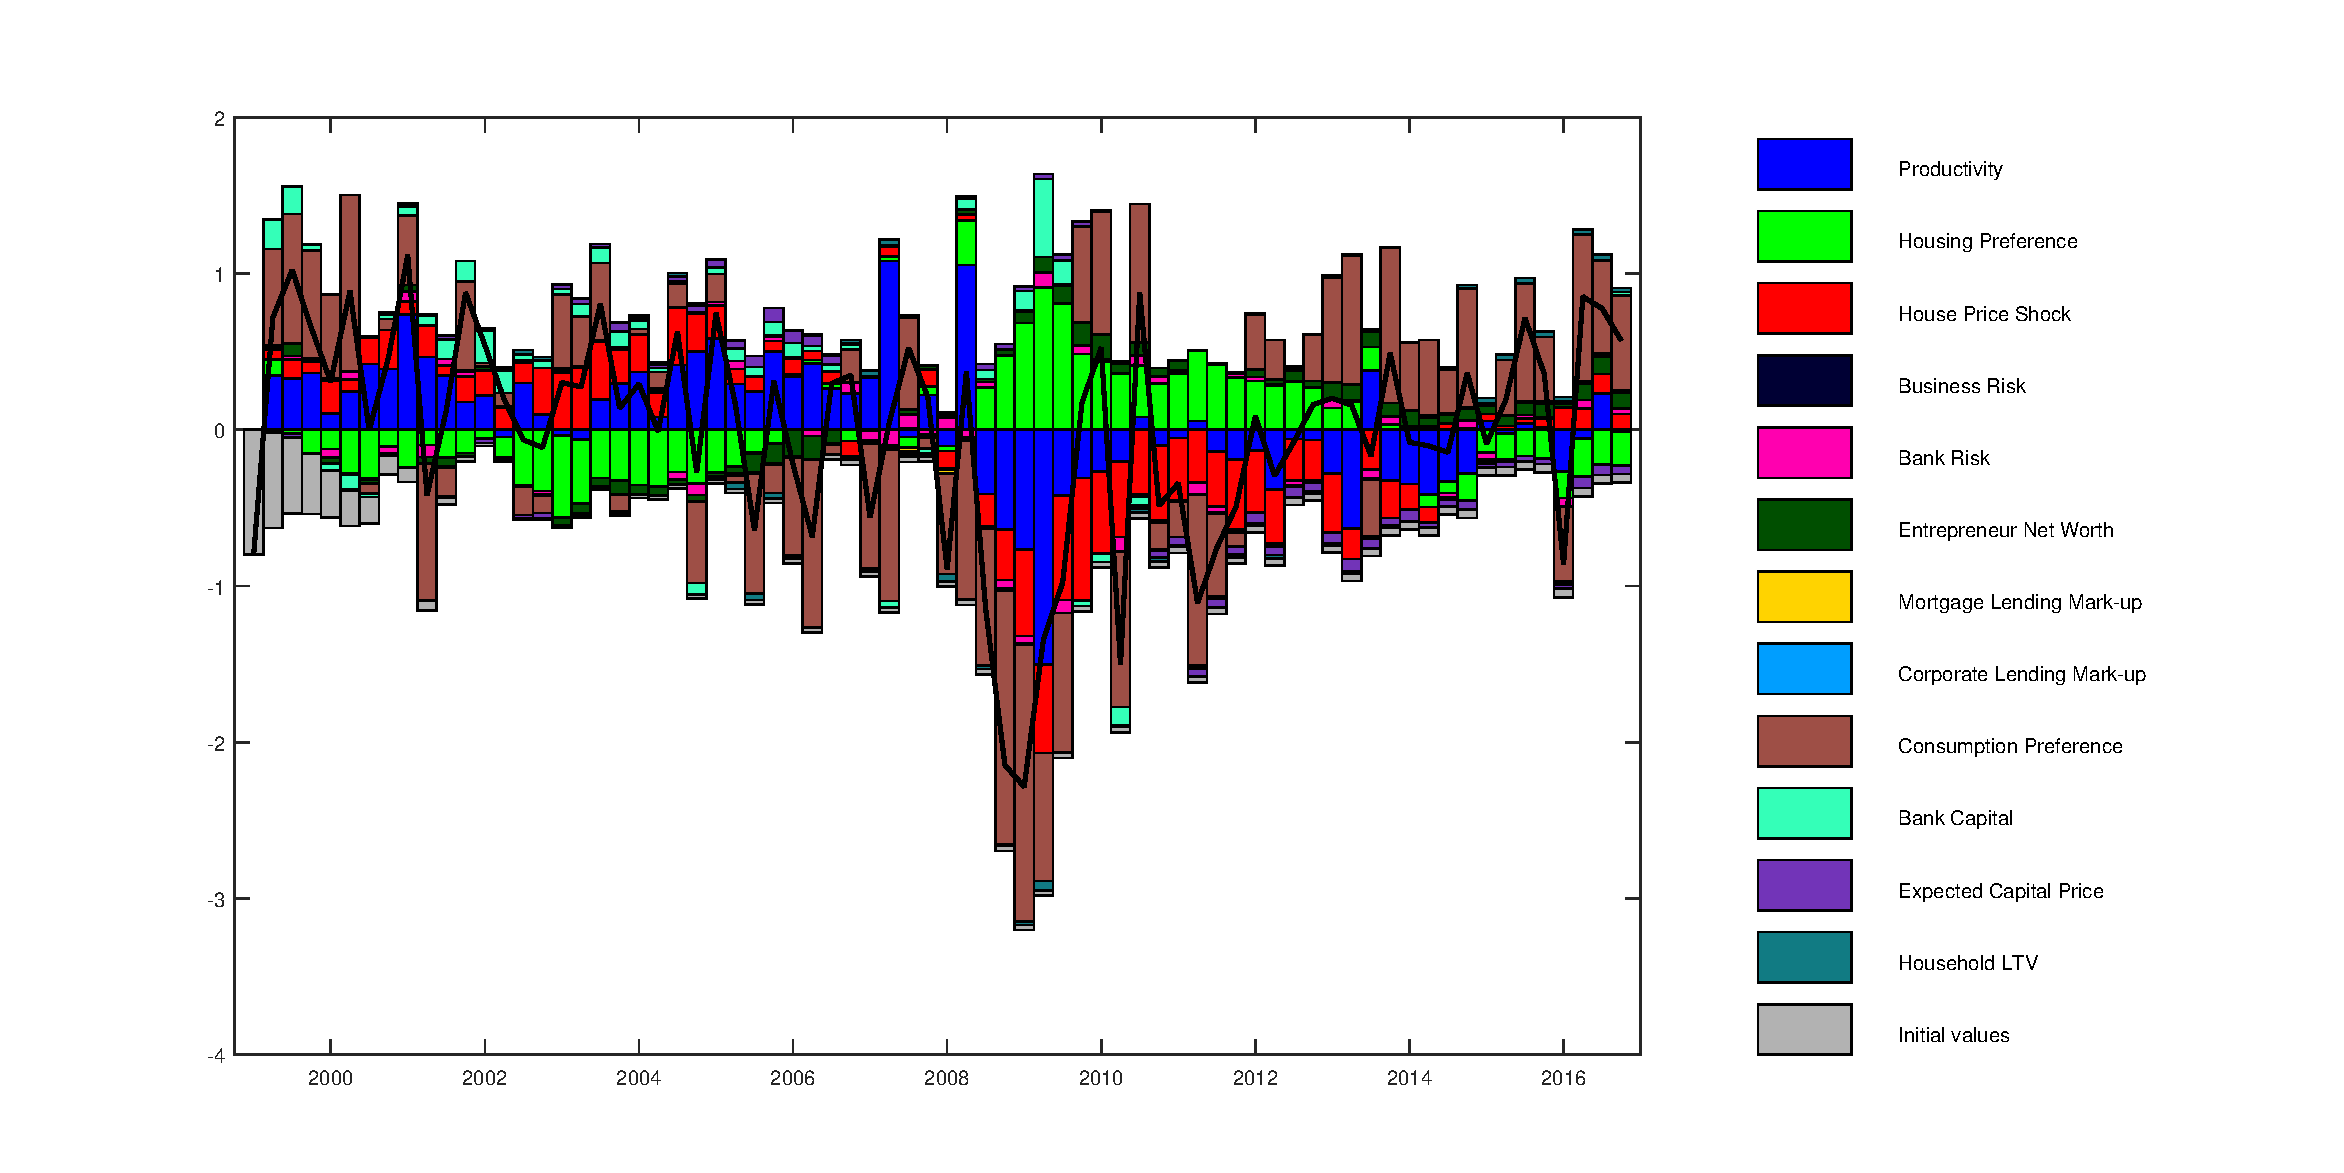
\includegraphics[scale=0.45]{decomp_dc.pdf}
%\end{figure}

%\begin{figure}[H]
%\centering
%\caption{Wage Growth}
%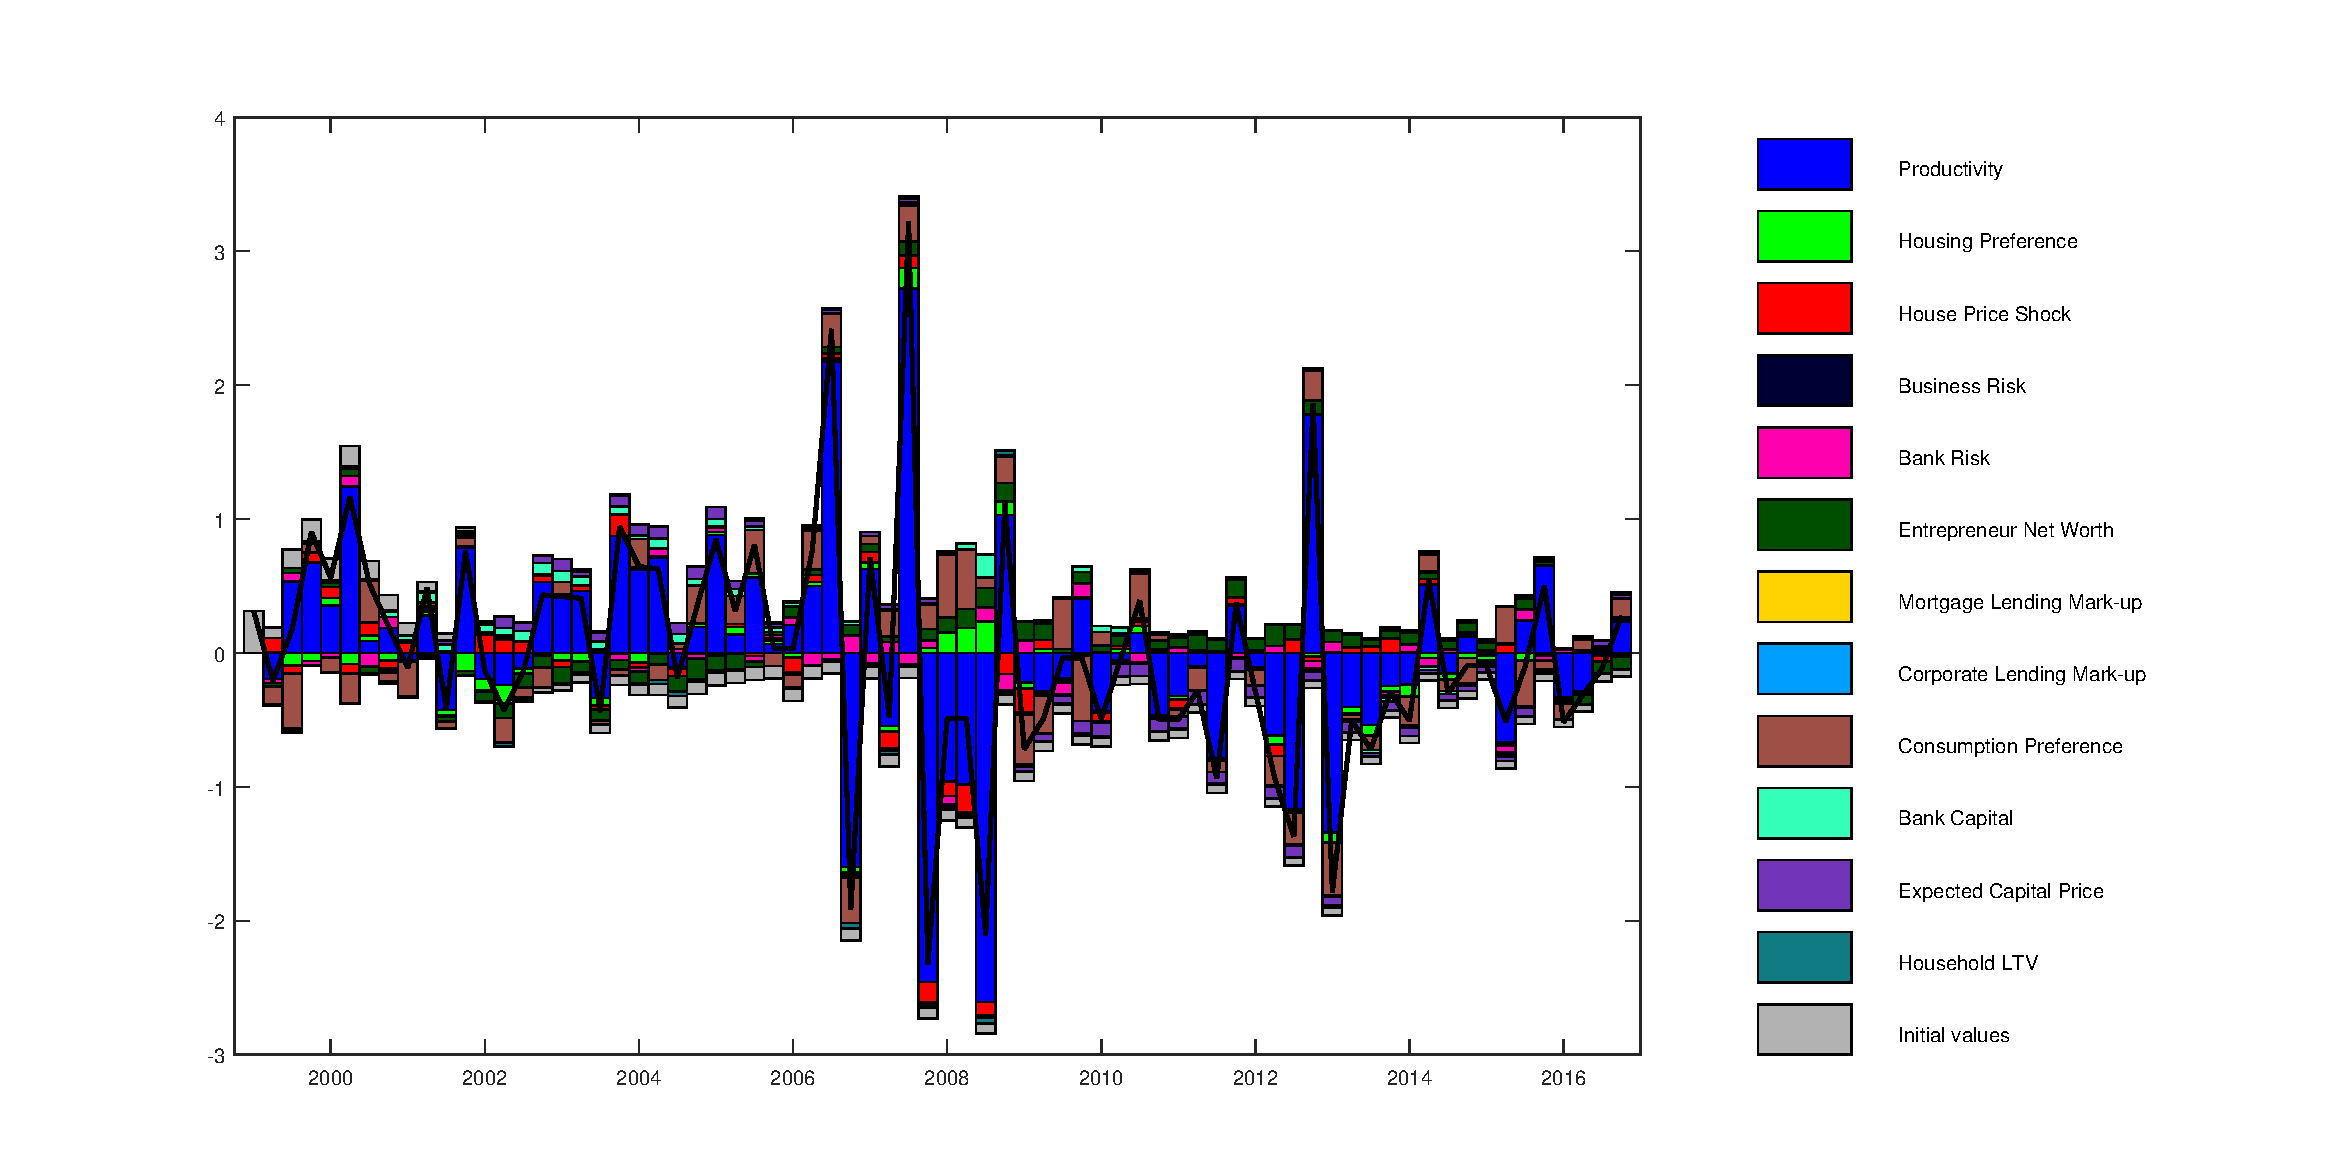
\includegraphics[scale=0.45]{decomp_dw.pdf}
%\end{figure}


\begin{table}[H]
\caption{Unconditional variance decompositions of key variables. The variables we consider are output growth  $\Delta y_t$ , house price growth  $\Delta q^H_t$, corporate lending growth    $\Delta b^e_t$, mortgage lending growth    $\Delta b^m_t$, wage growth   $\Delta w_t$,  and consumption growth   $\Delta c_t$ . }
\label{uncond_var_decomp}
\begin{tabular}{l|lllllll}
Shocks& $\Delta y_t$ & $\Delta q^H_t$  & $\Delta b^e_t$  & $\Delta b^m_t$  & $\Delta w_t$   & $\Delta c_t$  &    \\
\hline
\hline
Productivity & 17.58 & 0.85 & 12.26 & 1.78 & 88.53 & 21.07 &  \\
Housing Preference & 2.01 & 59.65 & 2 & 37.63 & 0.45 &  4.81 &  \\
Housing Price & 1.66 & 33.35 & 1.9 & 10.81 & 0.73 & 4.1 &  \\
Entr. Net Worth & 33.45 & 0.18 & 16.57 & 1.66 & 0.62 &  0.55 &  \\
Consumption Pref. & 31.65 & 4.49 & 1.08 & 11.33 & 7.58 & 66.21 &  \\
Exp. Capital Price & 3.63 & 0.07 & 39.8 & 0.28 & 0.28 &  0.19 &  \\
Other & 10.02 & 1.41 & 26.39 & 36.51 & 1.81 & 3.07 & 
\end{tabular}
\end{table}

\FloatBarrier




\section{Macroprudential Policy \& Welfare Analysis}

In this section we analyze the effects of macroprudential policy tools on household welfare, as well as our other target variables credit out and output. We discuss the effects of macroprudential tools in two steps: first, we focus on the steady-state of the model in isolation, without any business cycle fluctuations. Using this approach, we analyze the welfare-maximizing macroprudential policies individually and jointly, in order to determine whether the right combination of macroprudential tools can be welfare improving. Second, using the optimal policies from our steady-state analysis, we discuss a number of counterfactuals to see what effect the macroprudential policies would have had on the economy if they had been in place before the crisis. 

\subsection{Optimal Policy at the Steady State }


To assess the effect of macroprudential policies, we start by defining household welfare as follows: 

$$ W_t = \frac{W^s_t C^s_t + W^m_t C^m_t}{C^s_t + C^m_t} $$

where $W_t^i$  and $C_t^i$ with $i \in \{s,m \}$ refers to the welfare and consumption of patient and impatient households respectively. Accordingly, our welfare measure is a weighted average of patient and impatient households, where the weights are determined by the consumption shares of the households\footnote{This definition of welfare closely follows the version used in Mendicino et. al. (2018).}. Given this definition of aggregate welfare $W_t$, we use a simple liner-quadratic function as our objective:   

$$ E[W_t] - \omega \sqrt{Var[W_t]}.$$

Our motivation to include the welfare volatility in our objective function is to capture potential second-order effects of macroprudential policies, since our analysis of the model is based on a first-order approximation. Therefore we consider two cases for the weight on welfare volatility: $\omega=0$, which simply focuses on the expected welfare and ignores volatility, and $\omega=0.1$, which also puts a small weight on the volatility. 

We first find the optimal values of macroprudential tools when they are used individually. To this end, we use a grid search for each policy tool under consideration, leaving the other tools at their baseline level\footnote{For each tool, we use a grid length of 100. For housing LTV, we consider the range over $[0.7,0.95]$, while for SCRs and CARs, the range is $[0.05,0.25]$. For certain combinations of SCRs and CARs below $0.05$ the model becomes indeterminate, which is why we use this value as our lower bound.}. The results are reported in Table \ref{optimalPrud_1}. When $\omega=0$ (no weight on welfare volatility), we find that the optimal LTV is looser at $89.4 \%$ compared to its baseline level of $86 \%$, and it comes at a marginal welfare improvement of $0.014 \%$\footnote{Recall that the LTV limit in our model is assumed to be an always binding constraint. Our results on LTV here may be sensitive to the formulation of this, but we leave the occasionally binding LTV to future research.}. For the sectoral capital requirements (SCRr), we find relatively large optimal values (compared to the baseline of $11 \%$) of $20.7 \% $ and $15.5 \%$ for mortgage and corporate rates respectively, while the optimal CAR turns out to be $15.5 \%$. The welfare improvement among the three is largest when maximizing over mortgage SCR with $7.47 \%$ and smallest when maximizing over corporate SCR with  $15.5 \%$. As such, our results suggest that sectoral SCRs on mortgage lending is more important than those of corporate lending from a household welfare perspective. When we also place some weight on welfare volatility with $\omega=0.1$, we observe that the optimal LTV is tighter compared to $\omega=0.1$ and very close to its benchmark value of $86 \%$. Further, for both SCRs and CAR, we find smaller optimal values, suggesting a trade-off between welfare level and welfare-volatility. Nevertheless, these results indicate that there is a well-defined optimal policy in terms of LTVs, SCRs and the CAR. Table \ref{optimalPrud_fig} illustrates this result with respect to housing SCR and CAR: it is readily seen that the expected asggregate welfare  attains a maximum at the optimal values specified in Table \ref{optimalPrud_1}\footnote{The figures for welfare volatility, as well as for the LTV limit and corporate SCR are omitted here for brevity, but similar results follow.}.

Finally note the results on optimal CCyB, which follow mechanically: since the CCyB reacts to fluctuations of corporate and mortgage lending rates over the business cycle, it does not affect the steady-state levels of lending rates or welfare (i.e. the expected values of lending rates and welfare). Therefore, when there is no weight on welfare volatility, no optimal CCyB exists. At the other extreme, CcyB always reduces the volatility of lending rates and therefore volatility. Hence if there is any weight on volatility, the optimal CCyB is to simply set it as high as possible. 



\begin{table}[h]

\caption{Maximizing over prudential policy parameters, one at a time. LTV refers to housing loan-to-value limit only and we leave the corporate LTV at its baseline level of 86 \% throughout. The baseline policies are LTV$=86\%$, and CAR$=11 \% $ (i.e. both SCRs are set to $11 \%$). The numbers in parathesis indicate the improvement in aggregate welfare relative to the baseline.}
\label{optimalPrud_1}
\begin{tabular}{l|l|l|l}

 & $\omega$ & 0 & 0.1   \\
 \hline
 \hline
Parameter & & &  \\
\hline
\hline
LTV &  & 89.4 \% (0.014 \%) & 86.6 \% (0.001 \%)  \\

SCR-Mortgage &  & 20.7 \% (7.47 \%) & 17.6 \% (4.26 \%) \\

SCR-Corporate & & 15.5 \% (3.33 \%) & 16.7 \% (3.22 \%) \\

CAR & & 15.5 \% (5.11 \%) & 14.5 \% (3.82 \%) \\

CCyB & & NaN & Max. attainable \\

\end{tabular}
\end{table}


Given the individual optimal policies, we next investigate whether coordinating these policies (i.e. optimizing them jointly) may lead to further welfare improvements\footnote{CCyB is excluded from this exercise since it does not affect the welfare level as explained above.}. Table \ref{optimalPrud_2} reports the joint optimal combination of LTV, CAR and SCRs for the same cases with $\omega=0$ and $\omega=0.1$\footnote{For this exercise, we use a smaller grid size of 20 since the dimension of the problem is larger.}$^{,}$\footnote{Note that we effectively maximize over three policies, i.e. LTV and SCRs. The CAR is implicitly determined as the minimum of the two SCRs. }. With no weight on volatility, we find that optimal LTV is  looser compared to the previous case, with $91.25 \%$, mortgage SCR is higher than before with $21.25 \%$, and corporate SCR (and therefore CAR) reduces to its lower boundary of $5 \%$. With $\omega=0.1$, we now find that optimal LTV is even looser with $ 94 \%$, while sectoral SCrs are now at closer levels with $15.88 \%$ and $12.5 \%$ on mortgage and corporate lending respectively (and CAR is 12\%). The welfare improvements with the optimal combinations are $8.01 \%$ and $4.8 \%$ with $\omega=0$ and $\omega=0.1$ respectively, and this establishes our key result for this section: the appropriate combination of macroprudential tools achieves a better improvement on welfare compared to when the tools are used individually. 

Using these results, we next run a set of counterfactuals to analyze whether the macroprudential tools also achieve a better outcome over the business cycle. 


\begin{table}[h]

\caption{Maximizing over SCRs and LTV at the same time}
\label{optimalPrud_2}
\begin{tabular}{l|l|l|l}

 & $\omega$ & 0 & 0.1   \\
 \hline
 \hline
Parameter & & &  \\
\hline
\hline
LTV &  & 91.25 \%   &  94.06 \%  \\

SCR-Mortgage &  & 21.25 \%     & 15.88 \%   \\

SCR-Corporate & &  5(Min. attainable) \%  & 12.50 \%  \\

Welfare Improvement & & 8.01 \% & 4.8 \% \\

\end{tabular}
\end{table}




\begin{figure}[H]
\centering
\caption{Sectoral capital requirements on mortgage lending with a baseline of 11 \%. Welfare maximizing value is 20.7 \% with a weight of 0 on volatility. It decreases to 17.6 \% with a weight of 0.1 on the volatility.
\label{optimalPrud_fig}
\textbf{Welfare improvement: 7.47 \% and 4.26 \% respectively.} } 
\subfigure[Welfare level as a function of housing SCR.]{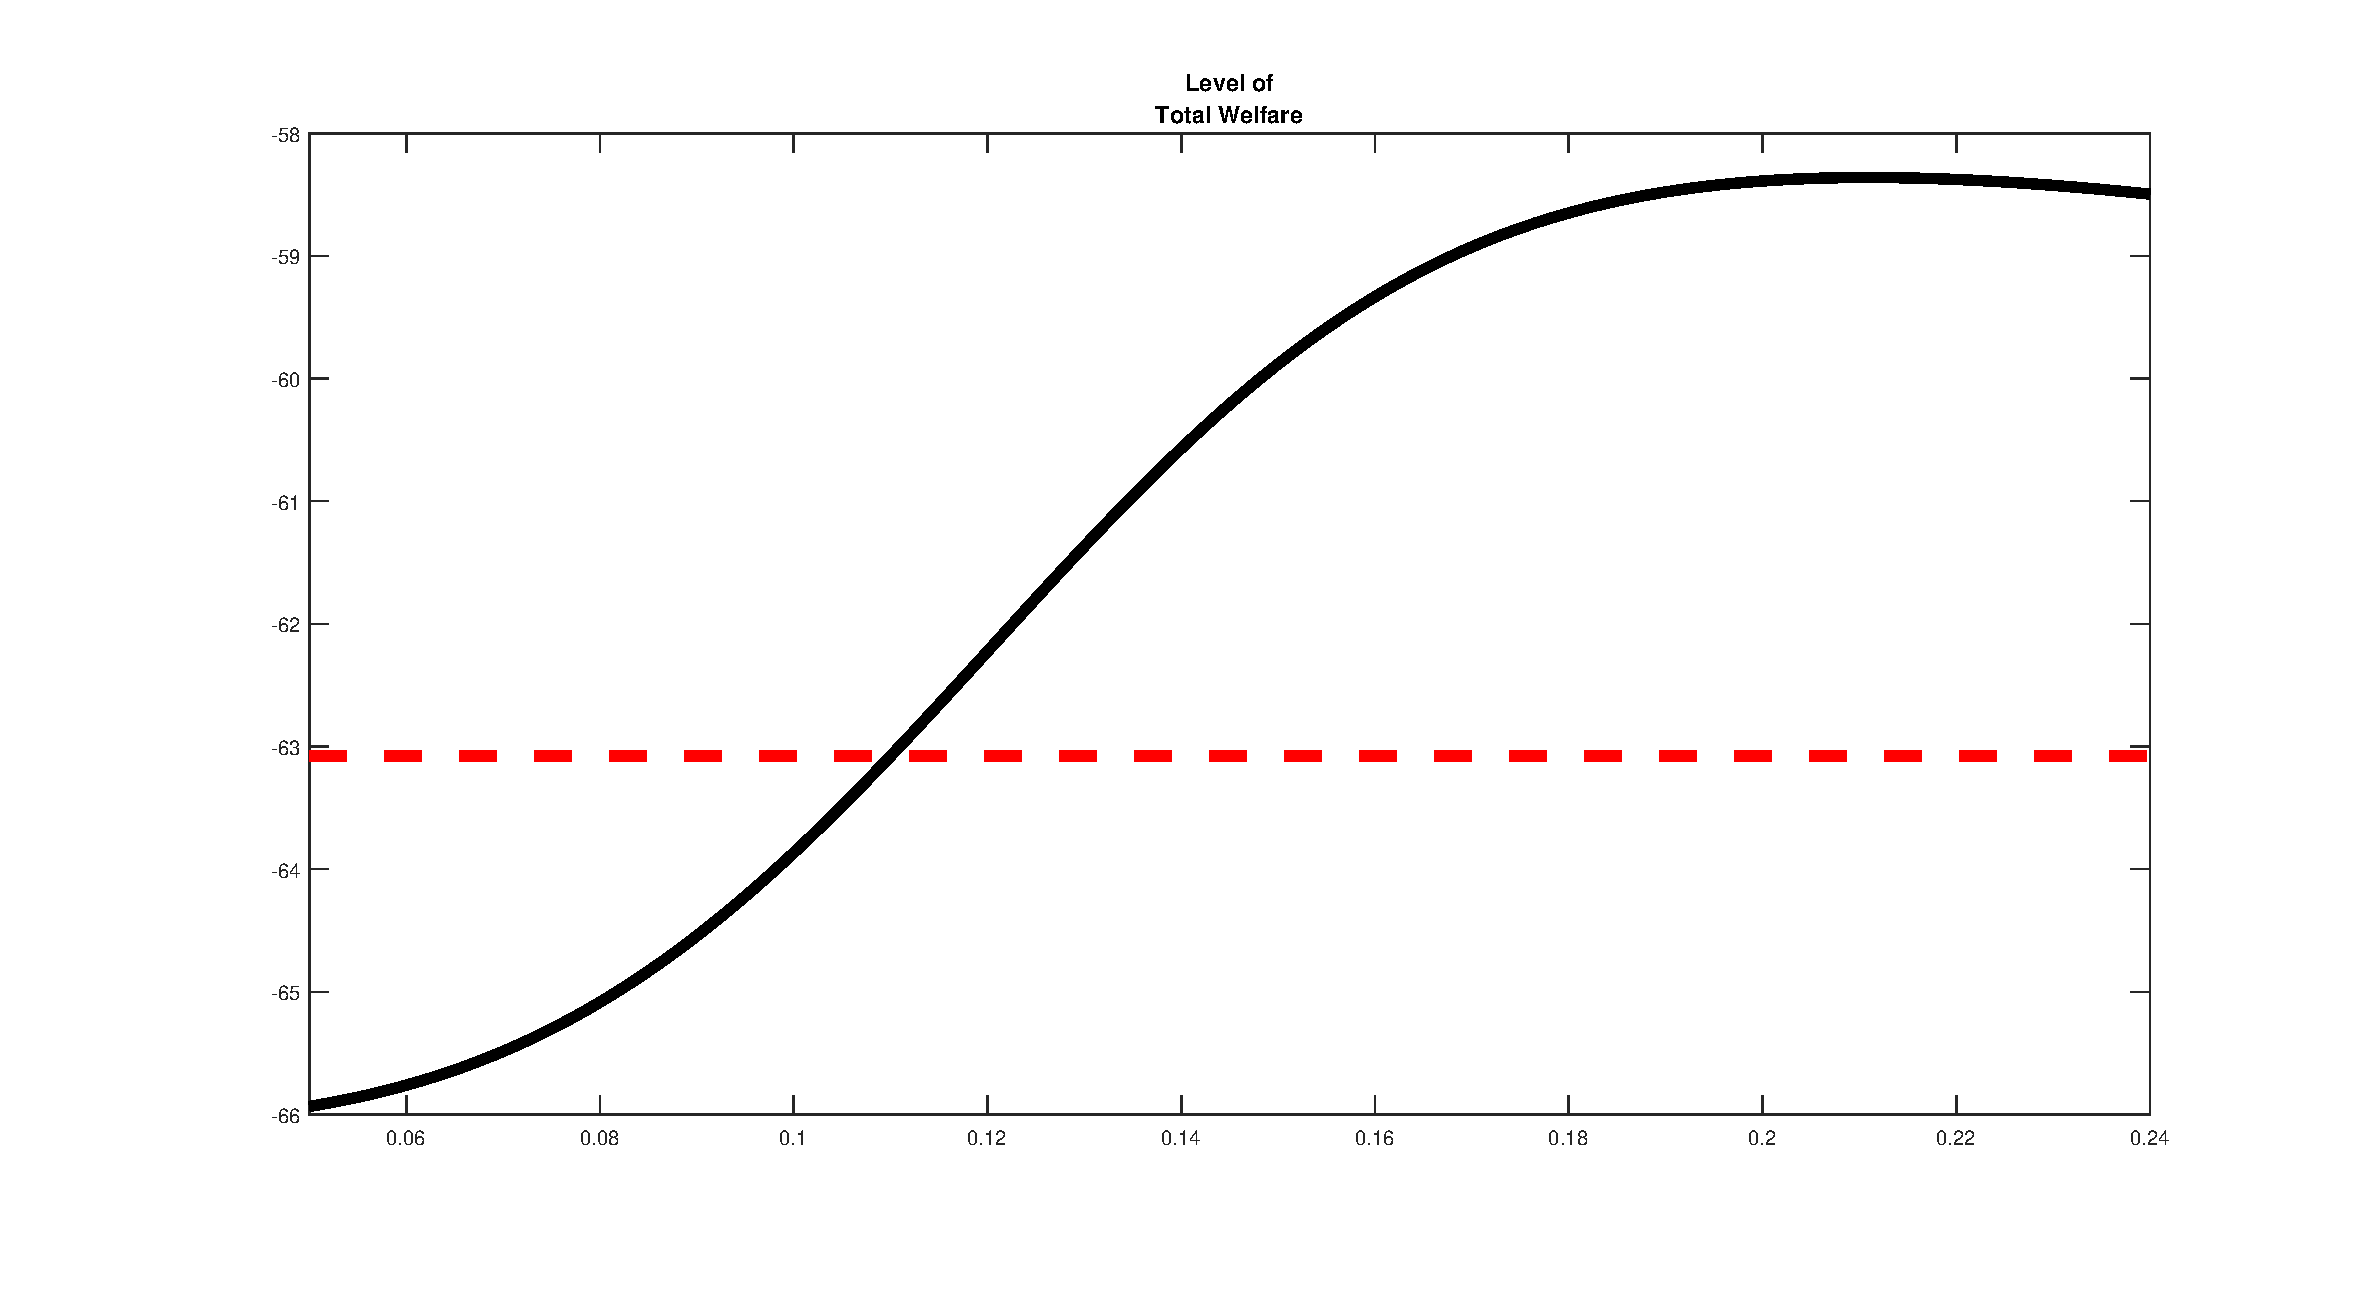
\includegraphics[scale=0.2]{welfare_SCR_housing_level.pdf}}
%\subfigure[Welfare volatility as a function of housing SCR/]{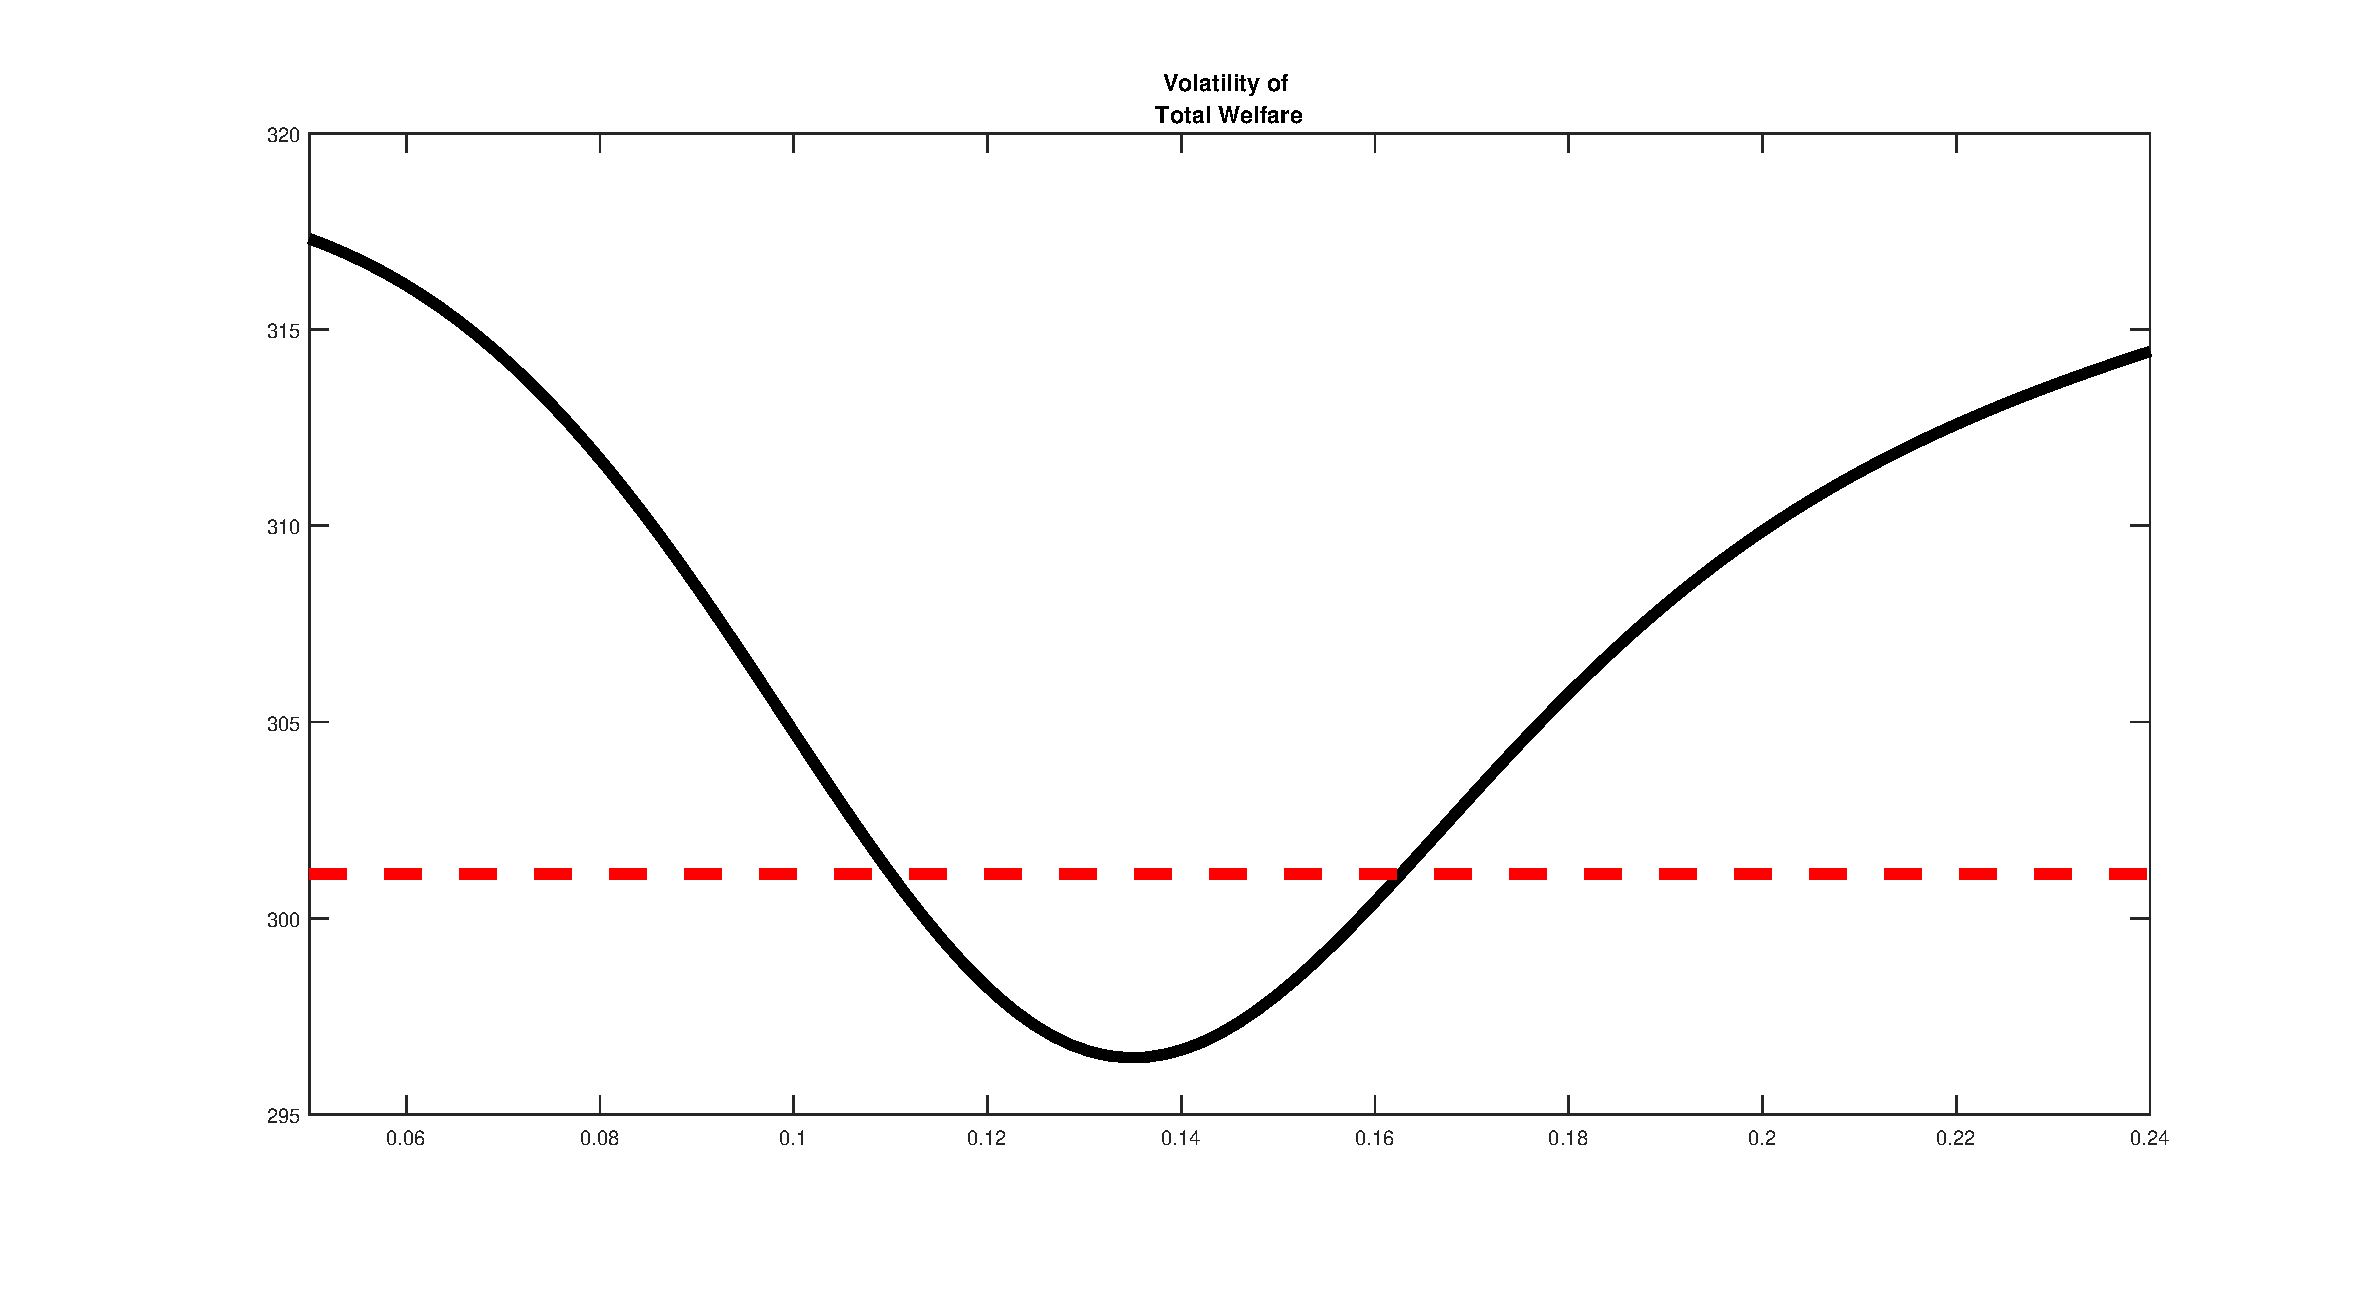
\includegraphics[scale=0.2]{welfare_SCR_housing_var.pdf}}\\
\subfigure[Welfare level as a function of CAR.]{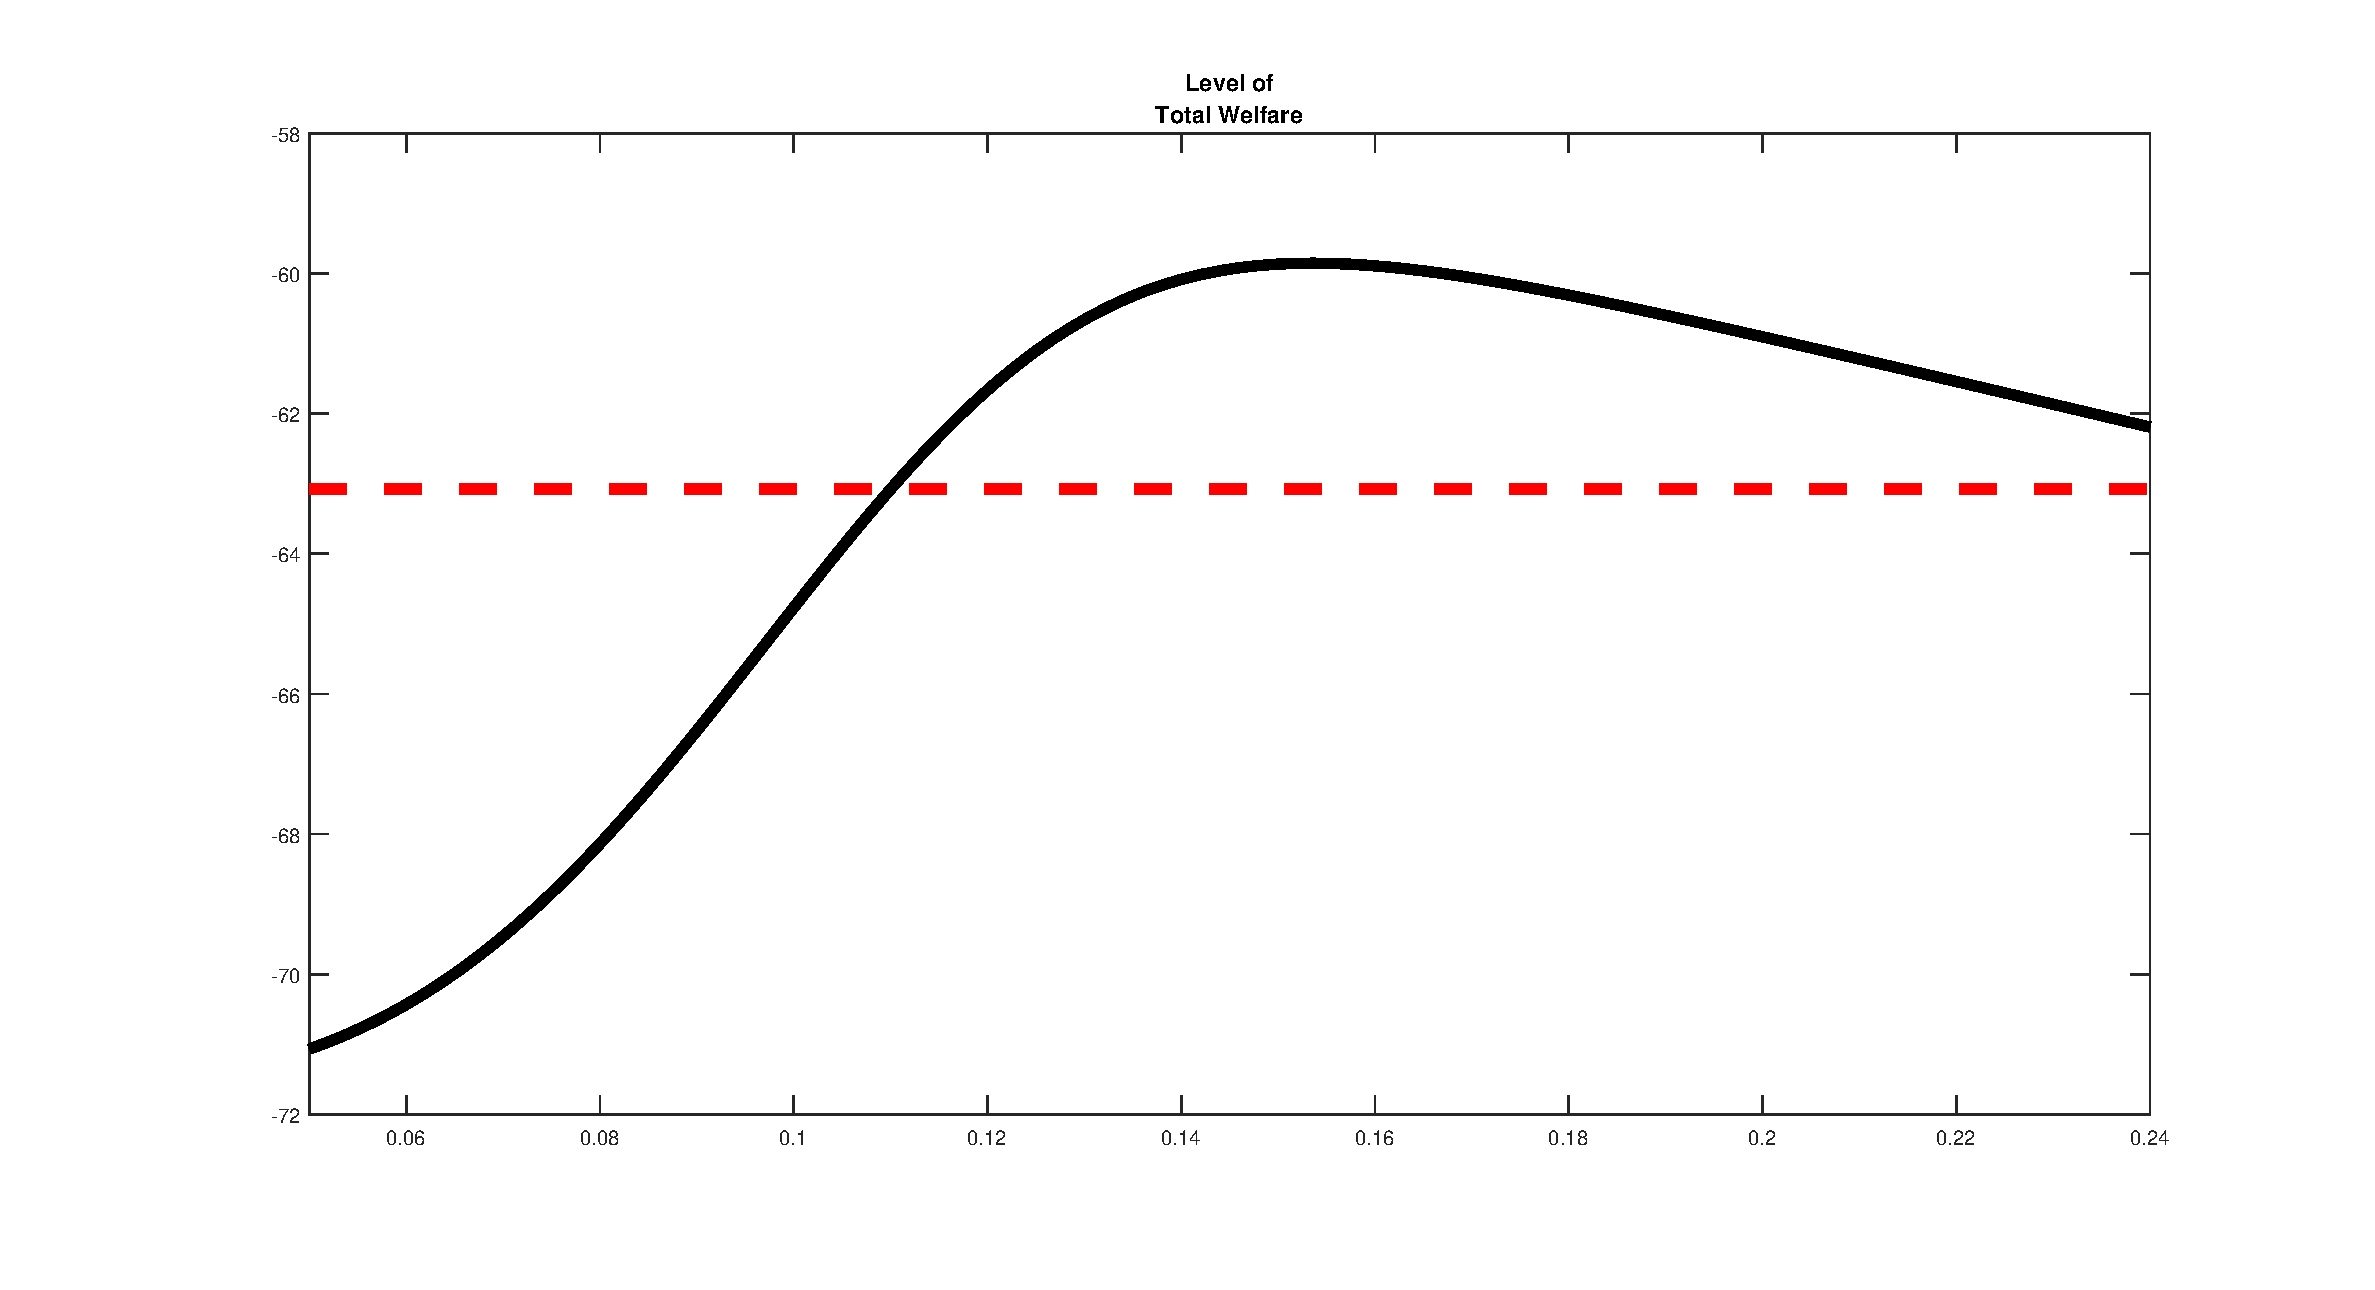
\includegraphics[scale=0.2]{welfare_CAR_level.pdf}}
%\subfigure[Welfare volatility as a function of CAR.]{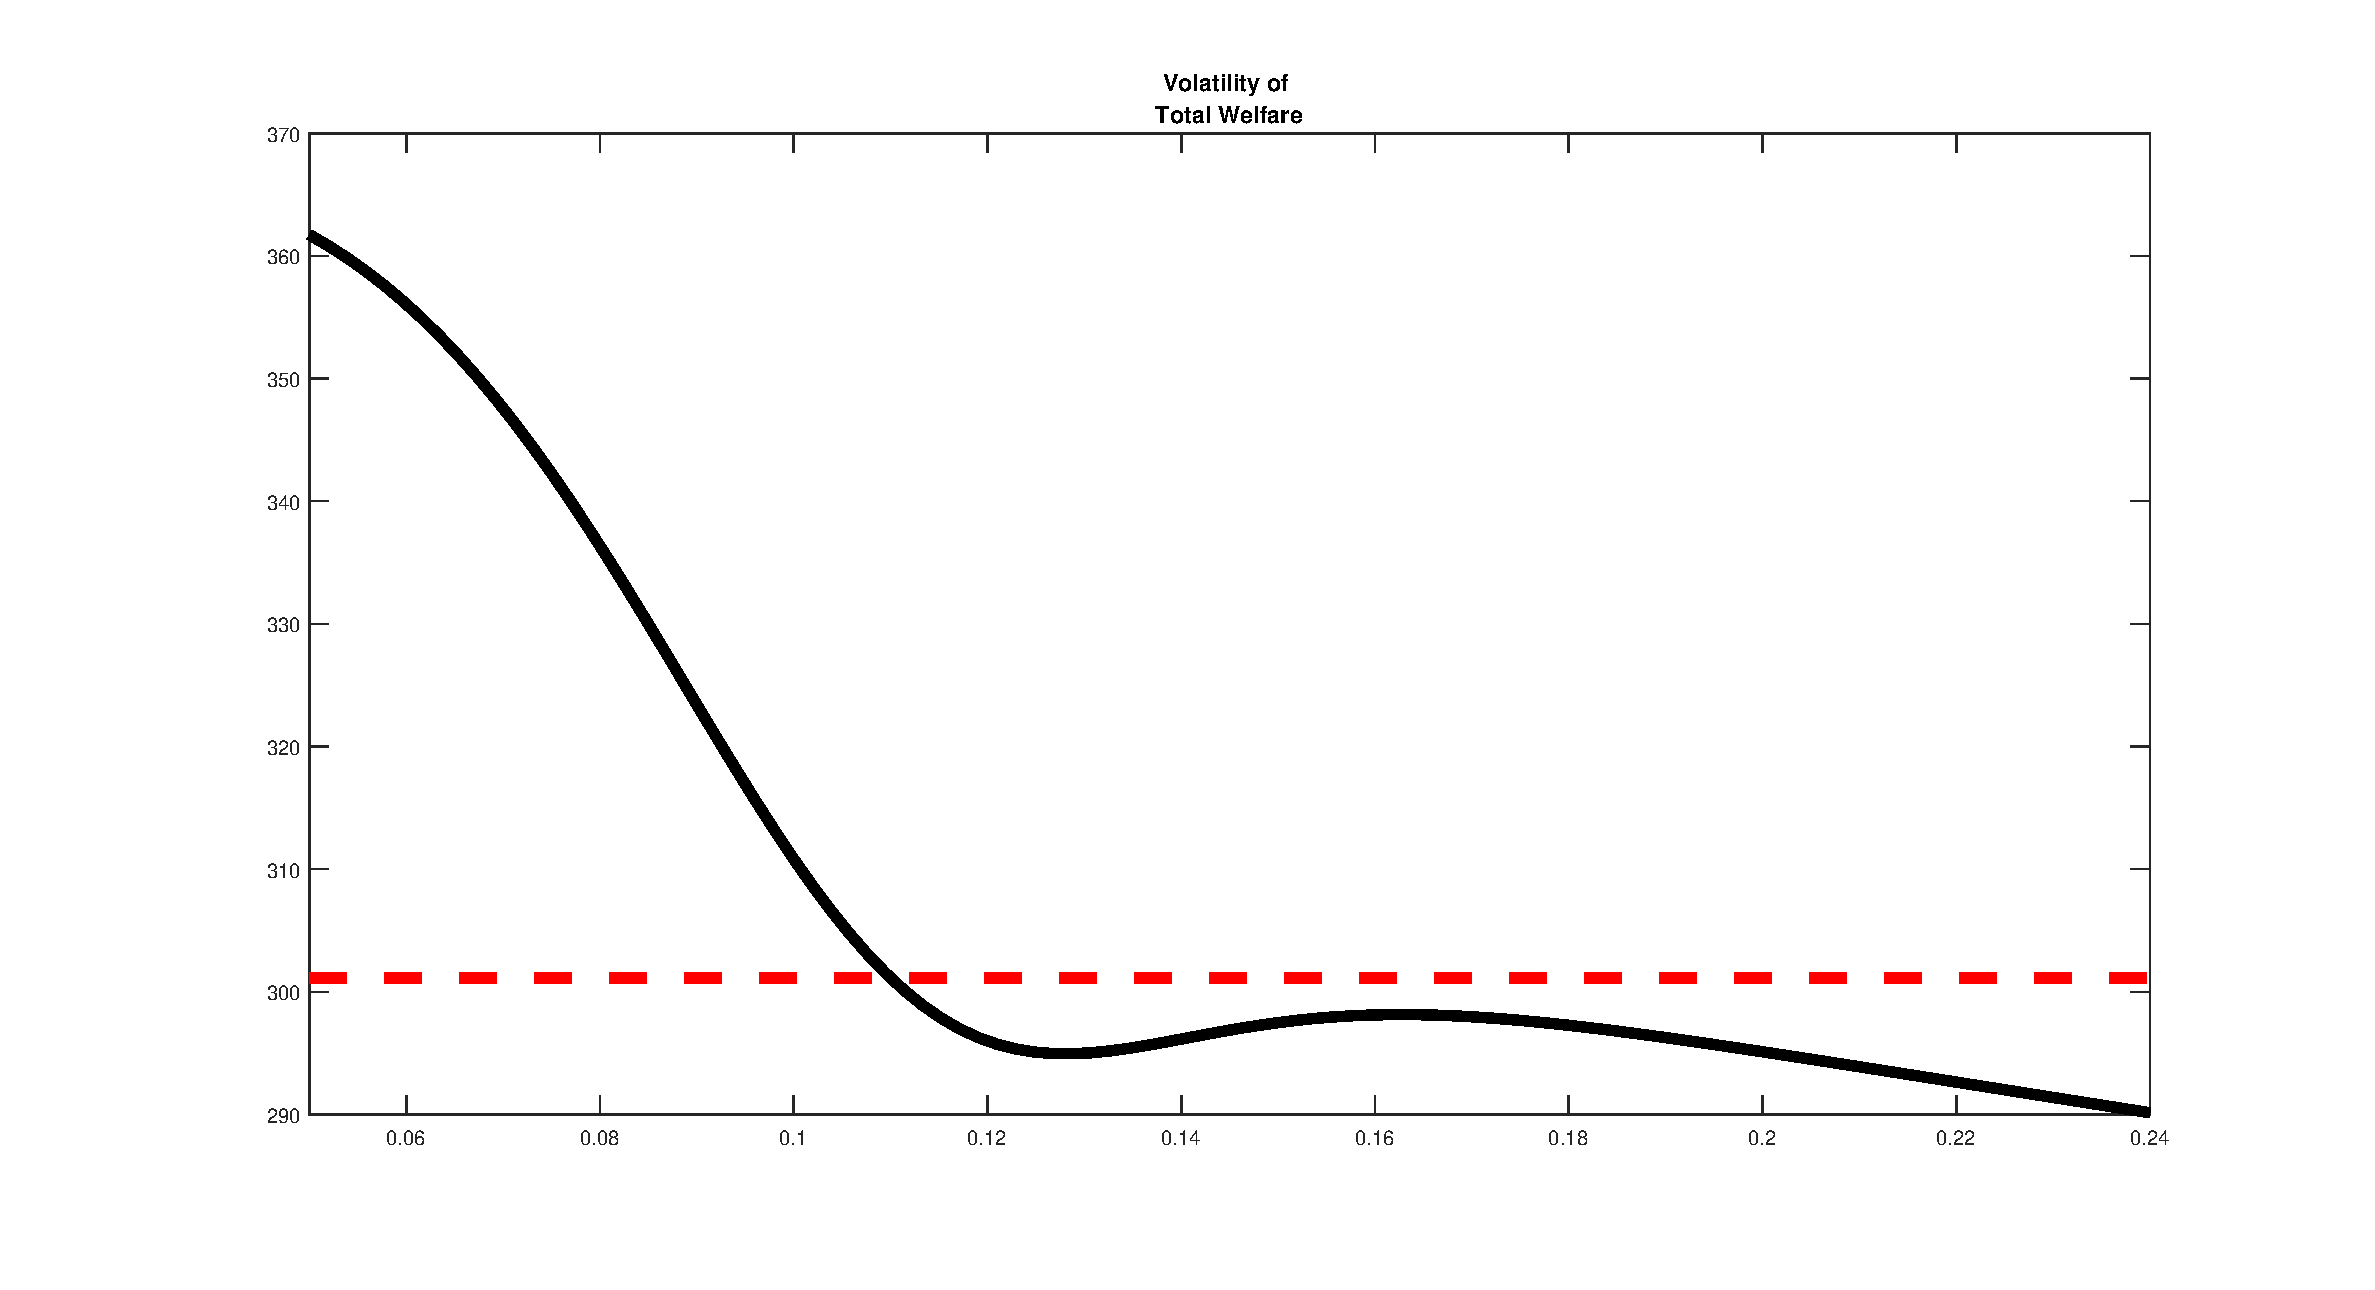
\includegraphics[scale=0.2]{welfare_CAR_var.pdf}}
\end{figure}




\newpage

\subsection{Counterfactual Simulations}

In this section we analyze what would have happened if different macroprudential tools were in place before financial crisis through the lense of our model. To this end, we use the joint optimal policies with $\omega=0.1$, hence we set the LTv limit to $94\%$, housing SCR to $15.8 \%$ and corporate SCR to $12.5 \%$. We use the parameters at the estimated posterior mode as reported in \ref{post_dist} and use the smoothed shocks at these parameter values. Accordingly, the shocks are fixed at these benchmark values, and we run the counterfactuals where the economy is hit by the same set of shocks, but macroprudential policies are set at their optimized levels.

 The first exercise assumes that the optimal policies are always in place from the beginning of the sample, which is reported in Figure \ref{counterfactual1}. As the values of these policies already make it clear, the optimal plan prescribes a looser borrowing constraint through a higher LTV limit compared to the benchmark scnerio, and a more resiliant bank through higher SCRs (and therefore CAR). This is exactly what comes out of our counterfactual simulation: due to higher capital requirements, the bank default rate decreases compared to the benchmark scenario. The higher housing SCR and looser LTV limit have opposing effects on household borrowing, and looking at the figure we observe that the looser LTV limit somewhat dominates, resulting in a higher household borrowing. While the corporate SCR is higher compared to the benchmark scenario, the relative increase is smaller compared to the housing SCR. This leads to a substitution effect on the bank's side, where the bank prefers to shift its portfolio from mortgage lending to corporate lending. It is readily seen that this substitution effect dominates the increase in the absolute level of corporate SCR (from 11 \% to 12.5 \%), and the business borrowing ends up higher under the counterfactual scenario compared to the baseline. The increased borrowing also boosts housing and capital investment, which feeds back into the consumption of both impatient (borrower) and patient (lender) households, as well as the aggregate output. The default rate of households increases under the counterfactual since the amount of borrowing is higher, but the disutility of this increased default rate is mostly offset by the utility of increased consumption and and lower bank default rate (which translate into a cost on the households). Therefore the borrowers are almost equally well-off under the counterfactual, while the lenders are better off due to increased consumption and investment. This results in a higher output and total welfare under our counterfactual scenario, even though the drops associated with the crisis are at similar levels compared to the baseline scenario. Accordingly, a looser borrowing limit combined with a more resilient bank results in an overall beneficial outcome. 

Looking at the percentage changes for our target variables in Figure \ref{counterfactual1}, it is readily seen that, the average volumnes of lending, as well as aggregate output and welfare are all higher under the counterfactual scenario. However, a similar level of drop after the financial crisis is still present in all variables. This suggests that, if different counterfactual policies were in place before the crisis, some aggregate indicators would have been improved but the crisis would not be prevented altogether. This is consistent with the policy of a looser borrowing constraint and a more resilient banking system, which does not aim to prevent the crisis but rather makes the system more resistant to it\footnote{An alternative policy analysis would involve the optimal scenario under a counterfactual simulation that finds the right balance between the level and volatility, which leave to future work.}. 



\begin{figure}[H]{}
\centering
\caption{Counterfactual I: using optimized values  with 0.1 weight on volatility. $\phi_H=15.8 \%, \phi_F=12.5 \%, \epsilon_H=94 \%$. For target variables, the average increases over the sample period are 4.9 \% for corporate credits, 4.2 \% for mortgage credits, 2.8 \% for output and 17.6 \% for households welfare.   }
\label{counterfactual1}
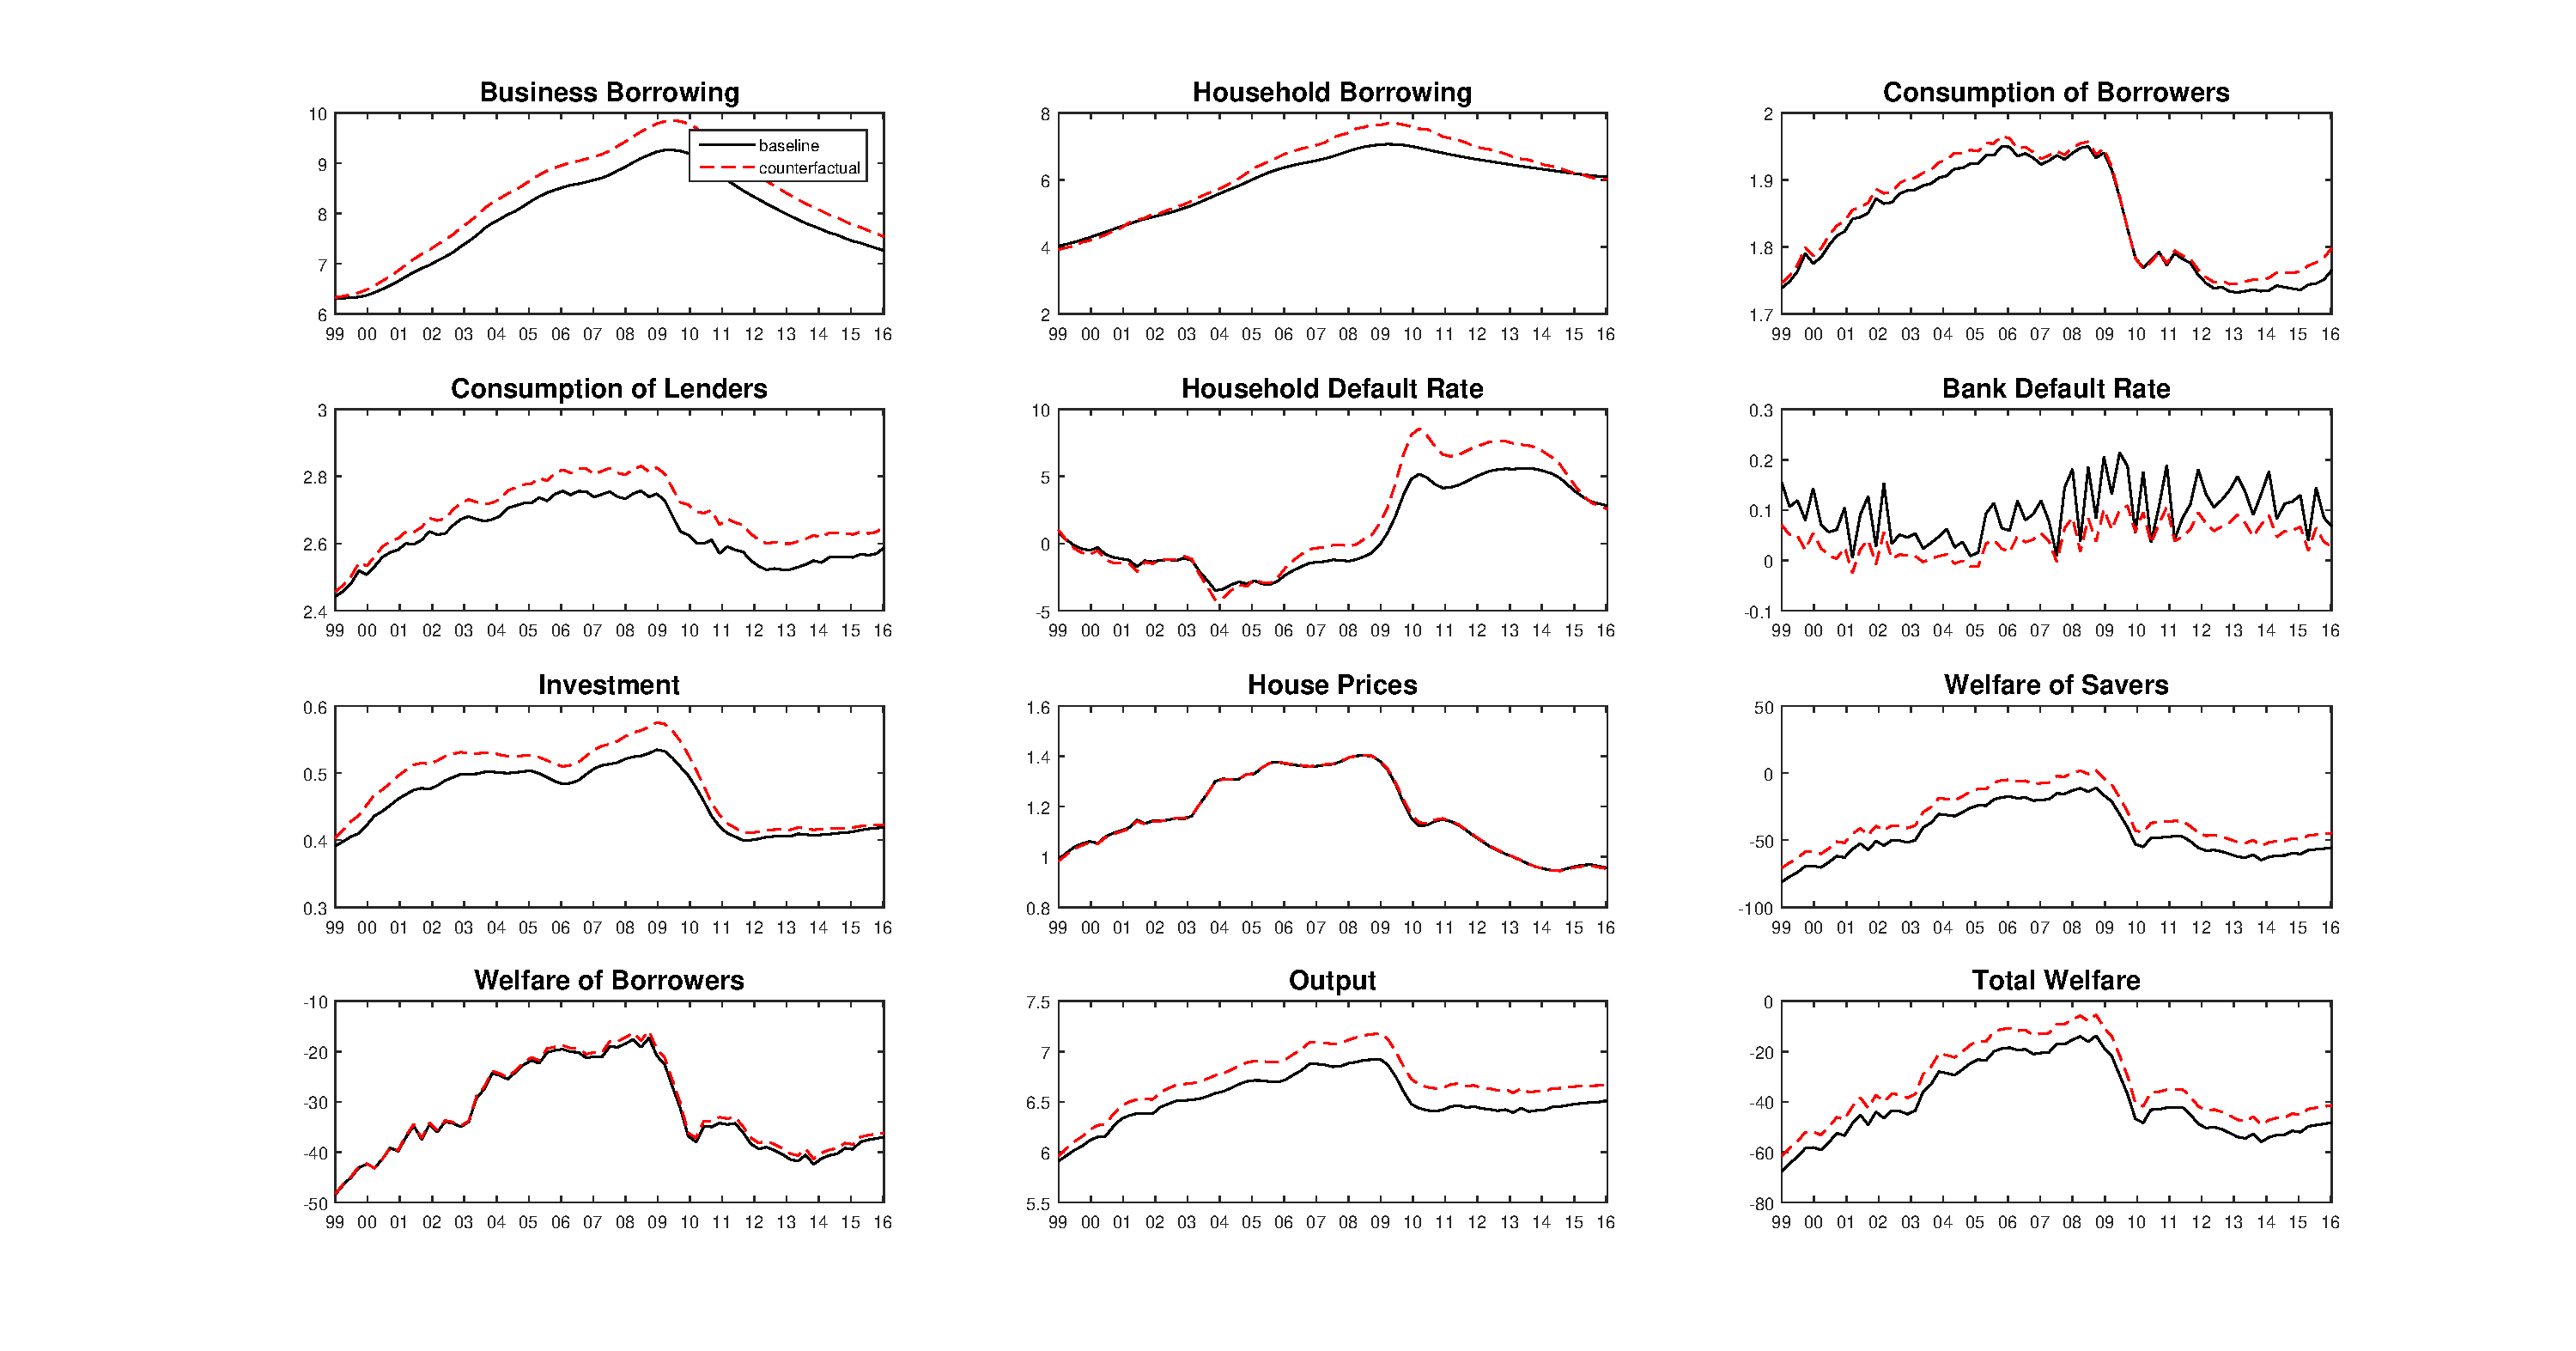
\includegraphics[scale=0.4]{main_counterfactual.pdf}
\end{figure}

%\begin{table}[h]

%\begin{tabular}{l|l|l}
%Variable & \% Change in Level & \% Change in Volatility \\
%\hline
%\hline
%    Corporate Credit           &       4.9    &      15 \\
%    Mortgage Credit            &      4.2    &       23 \\
%    Output         &     2.8    &    15.7 \\ 
%    Household Welfare       &     17.6     &     3.5\\
%\end{tabular}
%\end{table}


Next we consider a more realistic alternative scenario, where the same optimal policies are introduced over a 5-year period between 2001 and 2006. In this case we start from the benchmark policies in the year of 2001, and we gradually phase-in the policy levels to the optimal ones over this 5-year period\footnote{For this exercise, we introduce unit root shocks into the model on SCRs and the LTV limit. The policies are then phased-in in the form of permanent shocks.}. As might be expected, we obtain the same (positive) direction in all target variables both in terms of level and volatility, but the resulting magnitudes are substantially smaller since the policies are in place for a shorter duration. Nevertheless, we also obtain a socially beneficial outcome under the optimal policies. 

\begin{figure}[H]
\centering
\caption{Same counterfactual phased-in over a 5-year period over 2001-2006 in equal increments. For target variables, average increases  over the sample period are 2.4 \% for corporate credits, 0.8 \% for mortgage credits, 1.3 \% for output and 11.4 \% for household welfare.}
\label{counterfactual2}
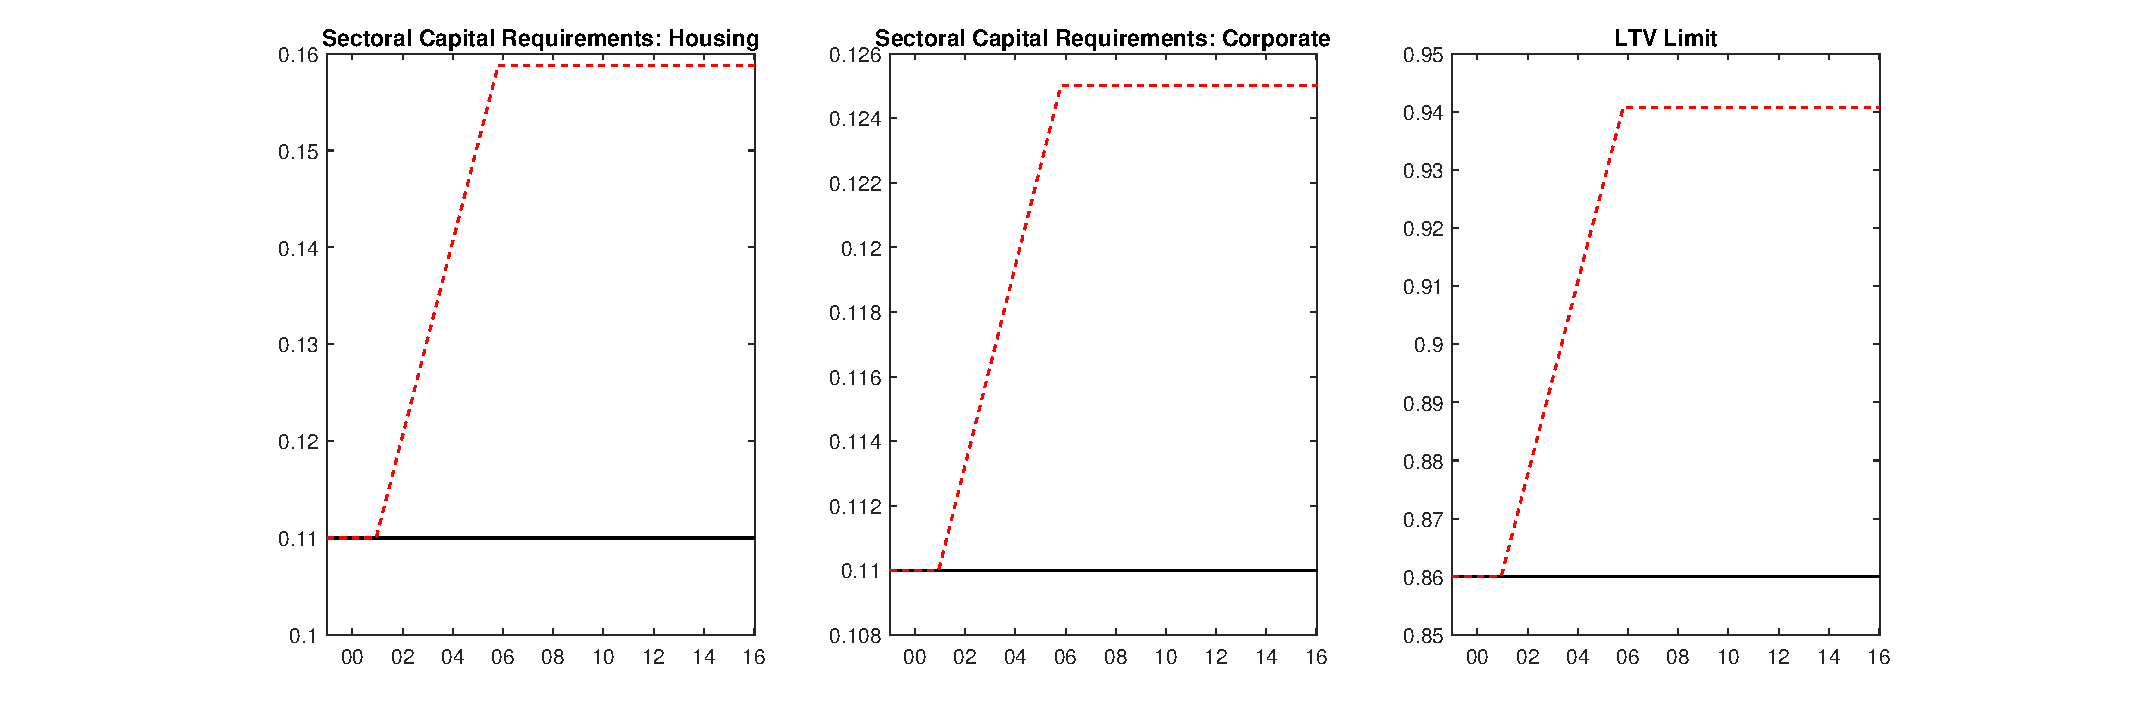
\includegraphics[scale=0.35]{CF_policy_rules10.pdf}
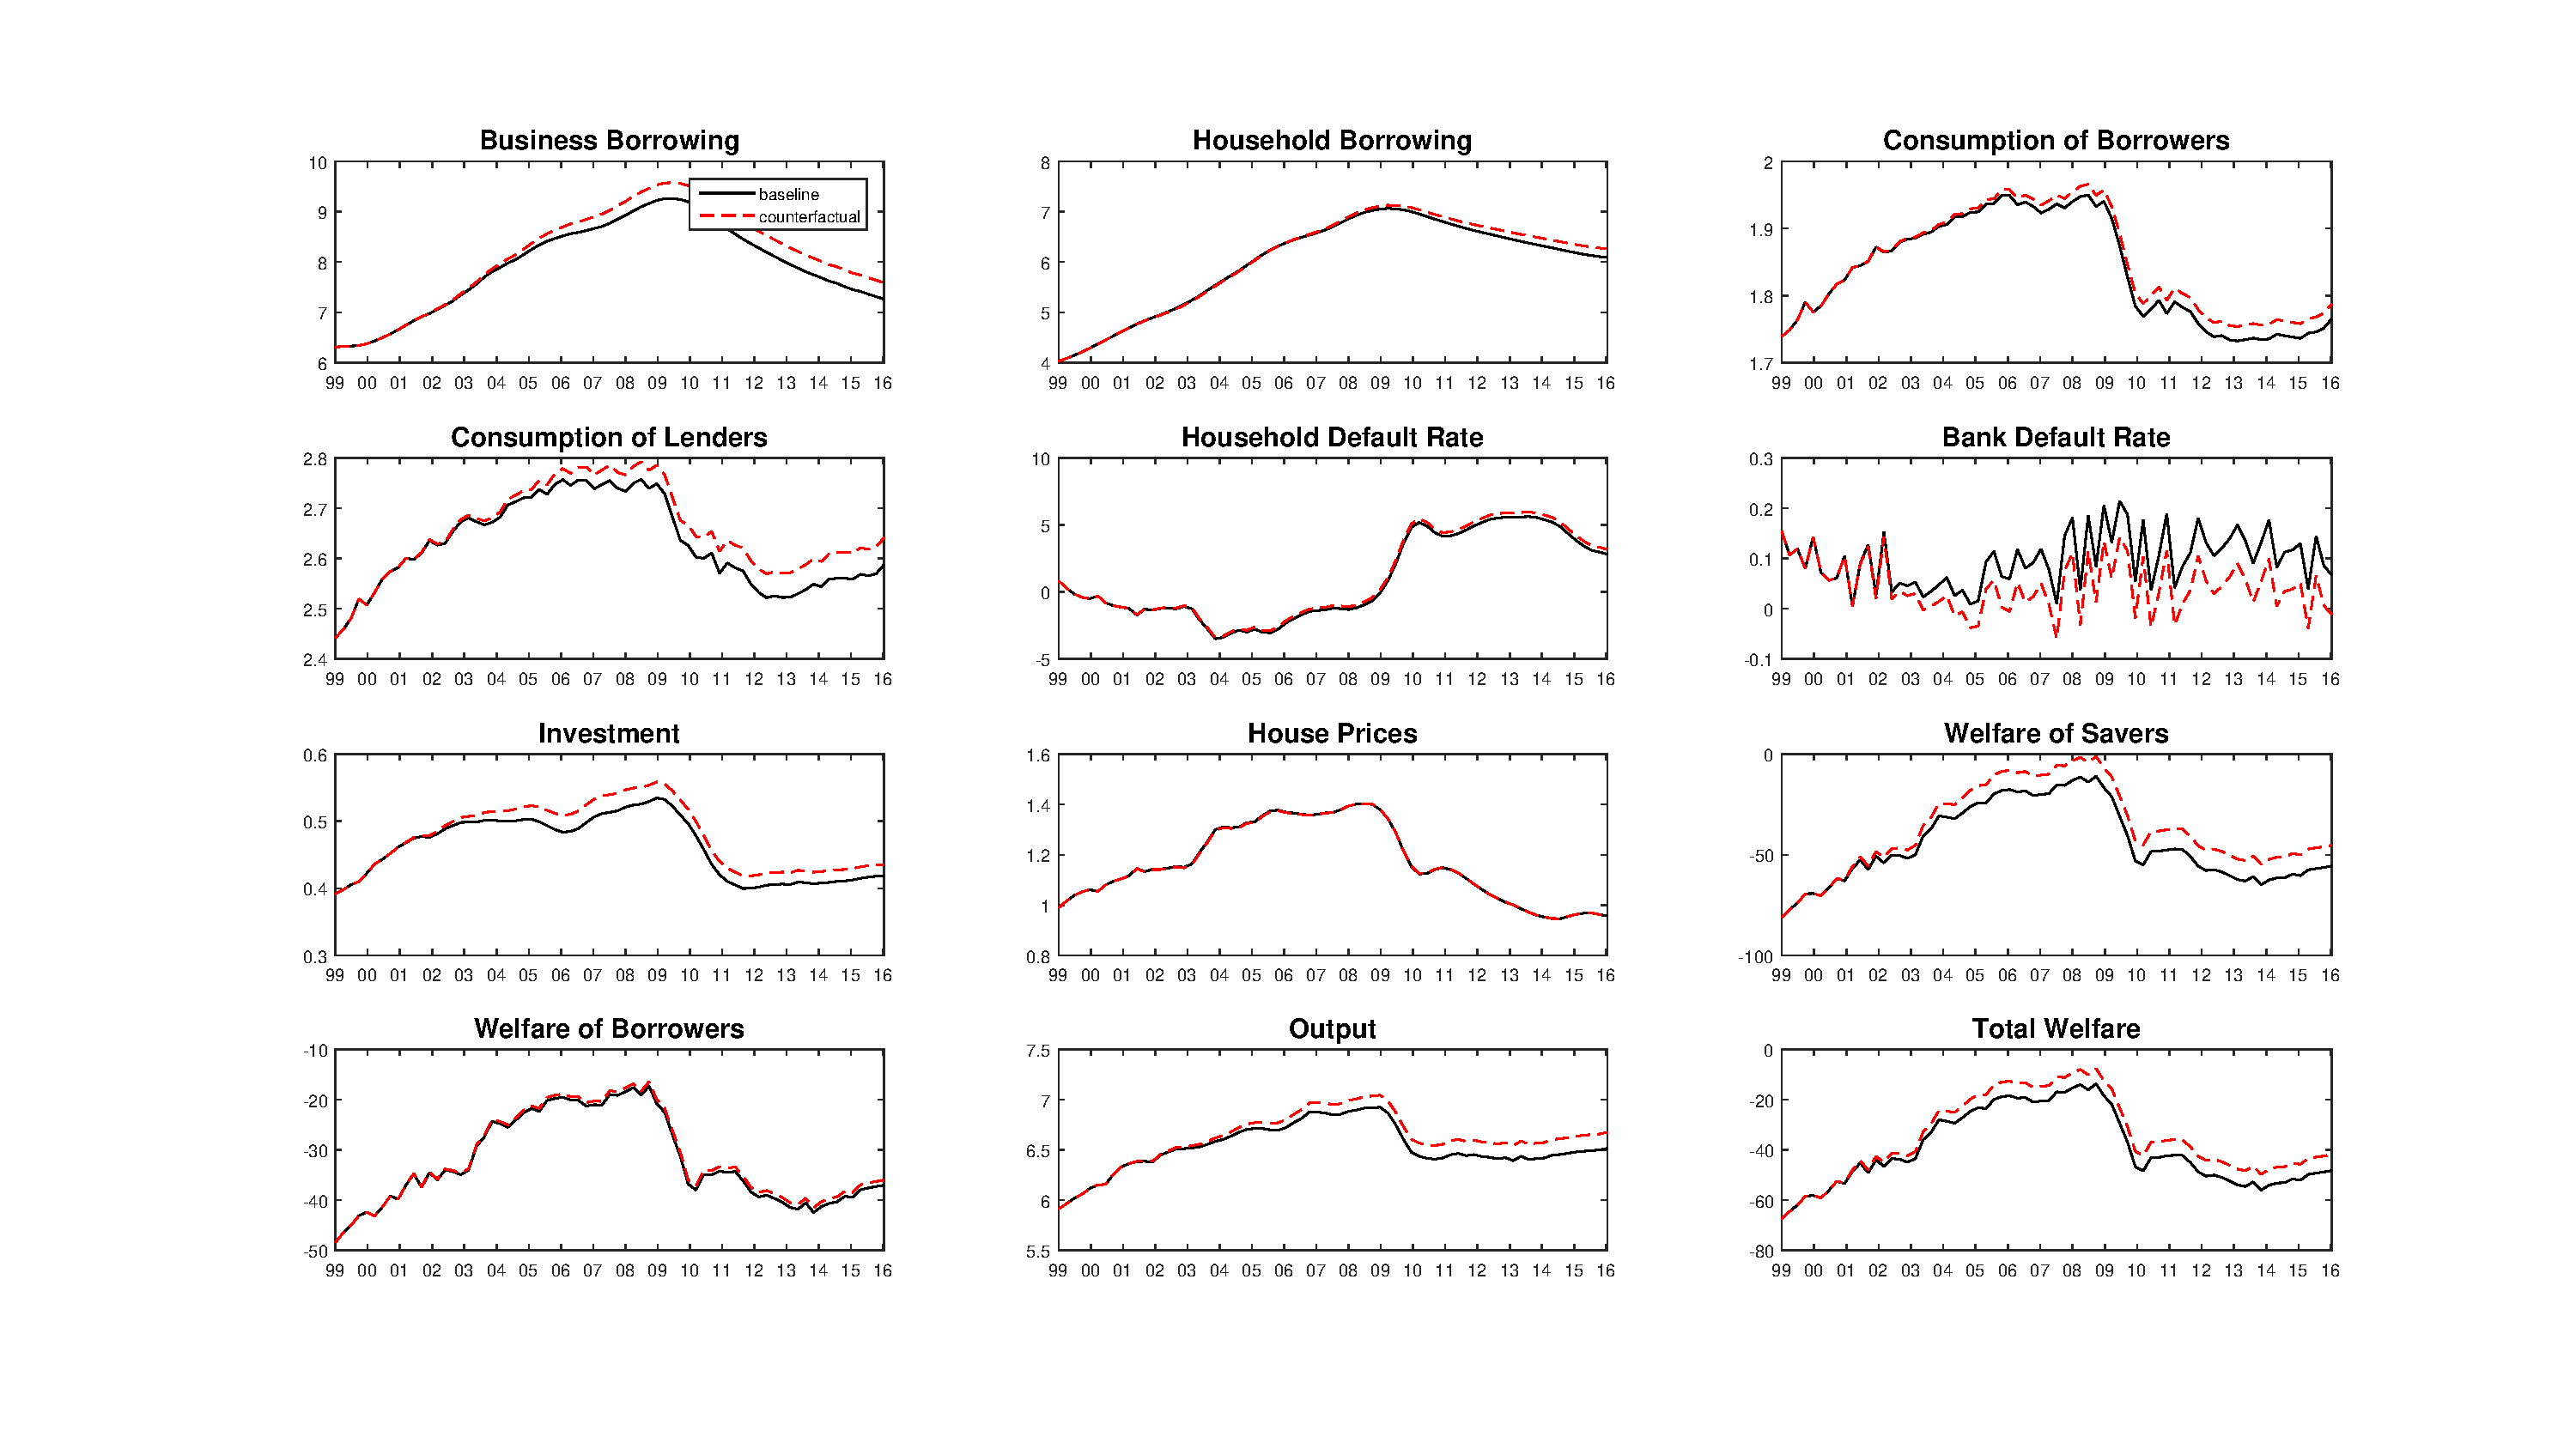
\includegraphics[scale=0.4]{main_counterfactual_phaseIn.pdf}\\

\end{figure}


%\begin{table}[h]



%\begin{tabular}{l|l|}
%\small
%Variable & \% Change in Level  \\% & \% Change in Volatility \\
%\hline
%\hline
%    Corporate Credit           &       2.4  \\% &      11 \\
%    Mortgage Credit            &      0.8     \\%&      4 \\
%    Output         				&     1.3   \\% &      10.7 \\ 
%    Household Welfare       &         11.4    \\%  &     7.3\\
%\end{tabular}
%\end{table}

Finally, to investigate whether CCyB improves the outcomes at the business cycle frequency, we analyze what happens with the introduction of CCyB when the optimal LTV and SCRs are already in place. To this end, we consider three scenarios with a sectoral CCyB individually, and when there is a CCyB in both sectors. Given our policy function, CCyB reacts to deviations of corporate and mortgage lending from its steady state level. We set the CCyB level to generate a standard deviation of approximately 2.5 \% in minimum requirements, which is obtained by tuning the reaction parameters in the policy function\footnote{This results in parameter values of $0.051$ for mortgage lending, and $0.128$ for corporate lending.}. The results are reported in Table \ref{counterfactual3}: we observe that introducing CCyB when the other optimal policies are already in place improves the outcomes further in terms of levels. In particular, aggregate output and welfare levels are improved when CCyB is active in both sectors, as well as when it is active in each sector individually. However, it is worth noting a downside with using CCyB in this form: during the sample period, the mortgage and corporate borrowing rates continue increasing above their steady-state levels during the pre-crisis period, and while they start declining with the onset of the crisis, they are still well above their steady-state values once the crisis hits, and they remain above that level throughout the whole sample. As such, a CCyB that reacts  to deviations of borrowing rates from their steady-state level prescribes ever-increasing capital requirements throughout the sample period. This issue exaggerates the volatility impact of CCyB, and could be resolved with alternative reaction functions such as a CCyB on the growth rate of lending rates. We leave such alternative formulations to future research. 


\begin{table}[h]
\caption{Does CCyB improve things when optimal SCRs are in place?}
\label{counterfactual3}
\begin{tabular}{ll||ll}
\small
Variable & \% Change in Level  & Variable & \% Change in Level \\
\hline
Baseline optimal SCR+LTV & &  CCyB 2.5 \%, mortgages   \\
\hline
    Corporate Credit           &       4.9  &    Corporate Credit           &       7.3   \\
    Mortgage Credit            &      4.2 & Mortgage Credit            &       0.05\\
    Output         &     2.8   &  Output         				&     3.9  \\
    Household Welfare       &     17.6 &   Household Welfare       &        19.4  \\
\hline
CCyB 2.5 \%, both sectors &   &   CCyB 2.5 \%, corporate  \\
\hline
    Corporate Credit           &       5.8  &  Corporate Credit           &       3.2 \\
    Mortgage Credit            &       4.5  &    Mortgage Credit            &       8.1  \\
    Output         				&     4.1  &  Output         				&      2.7  \\
    Household Welfare       &        21.2  &  Household Welfare       &          19.1  \\
\hline

\end{tabular}
\end{table}



\begin{comment}

\begin{table}[h]
\caption{Does CCyB improve things when optimal SCRs are in place?}
\label{counterfactual3}
\begin{tabular}{l|l}
\small
Variable & \% Change in Level \\ % & \% Change in Volatility \\
\hline
Baseline optimal SCR+LTV &  \\ % & \\
\hline
    Corporate Credit           &       4.9 \\ %  \%    &      15 \\
    Mortgage Credit            &      4.2 \\ %    &       23 \\
    Output         &     2.8  \\ %   &    15.7  \\ % \\ 
    Household Welfare       &     17.6   \\ %   &     3.5\\
\hline
CCyB 2.5 \%, both sectors & \\ %  & \\
\hline
    Corporate Credit           &       5.8  \\ %   &     17 \\
    Mortgage Credit            &       4.5  \\ %  &      26 \\
    Output         				&     4.1   \\ %  &     27.7 \\ 
    Household Welfare       &        21.2  \\ %    &     7.54\\
\hline
CCyB 2.5 \%, mortgages  & \\ %  & \\
\hline
    Corporate Credit           &       7.3  \\ %   &     27.3 \\
    Mortgage Credit            &       0.05 \\ %  &      9.7 \\
    Output         				&     3.9  \\ %   &     27.5 \\ 
    Household Welfare       &        19.4  \\ %    &     5.9\\
 \hline
CCyB 2.5 \%, corporate  & \\ %  & \\
\hline
    Corporate Credit           &       3.2  \\ %   &     4.5 \\
    Mortgage Credit            &       8.1  \\ %   &     39 \\
    Output         				&      2.7   \\ %  &    13.4 \\ 
    Household Welfare       &          19.1  \\ %   &    4.71\\   

\end{tabular}
\end{table}

\end{comment}

\FloatBarrier


\section{Impulse Response Analysis}

\subsection{Interest Rate Stickiness and Shock Propagation}

In this section we discuss the effects of individual shocks on key variables through impulse response functions. We first start with the effects of interest rate stickiness on shock propagation. Given the significant rate of stickiness on U.K. data, this can be an important channel that affects the transmission of shocks throughout the economy. We focus on three shocks across different sectors of the economy, namely a housing preference shock on the housing side, an expected capital price shock on the corporate side and a bank capital shock on the banking side. We report the effects on several key variables with and without interest rate stickiness in each sector, in particular we focus on four scenarios in terms of interest rate stickiness: (i) estimated degrees of stickiness, (ii) a low degree of stickiness in the housing sector, (iii) a low degree of stickiness in the corporate sector and (iv) a low of degree stickiness in both sectors. 

Figure \ref{irf_stickiness_J} reports the effects of a negative housing preference shock: the shock directly lowers the demand for borrowing by households, which translates into a drop in house prices. Since the shock leaves the level of household wealth unchanged, they increase their consumption spending. The effects on these three variables are similar with different degrees of stickiness, since the shock originates in the household sector and does not transmit through interest rate. In response to the drop in housing demand, the bank lowers the household interest rate and this is where we start to see the effects of interest rate stickiness: it is able to cut the interest rates the most when interest rate stickiness is low in both sectors, while the drop in interest rates is smallest when the stickiness is at the estimated level in both sectors. 
In response to the drop in house prices, aggregate investment, which consists of housing and capital investment, also decreases subject to a similar constraint as the housing sector depending on the degree of stickiness. Similar to the household interest rates, the bank also ends up lowering corporate rates for two reasons: first, keeping the corporate rates constant while lowering mortgage rates would result in a substitution effect into the housing sector, and therefore the bank has an inventive cut corporate rates in response to mortgage rates. Second, the volume of business borrowing decreases given the lower aggregate investment, and therefore the bank prefers lower business lending rates to make up for the loss in demand.  The net effect on aggregate output in general depends on the positive effects on aggregate consumption and the negative effects on aggregate investment. Under our parameterization, the negative effects dominate and we see a reduction in aggregate output following the housing preference shock. The effect is smallest when the degree is stickiness is small in both sectors, and the stickiness in mortgage rates has the highest impact on aggregate output in this case. This is intuitive since the shock starts from the housing sector, and hence the largest spillover effect takes place when the bank is unable to react through mortgage rates. 




\begin{figure}[H]
\centering
\caption{Impulse responses to a negative housing preference shock.}
\label{irf_stickiness_J}
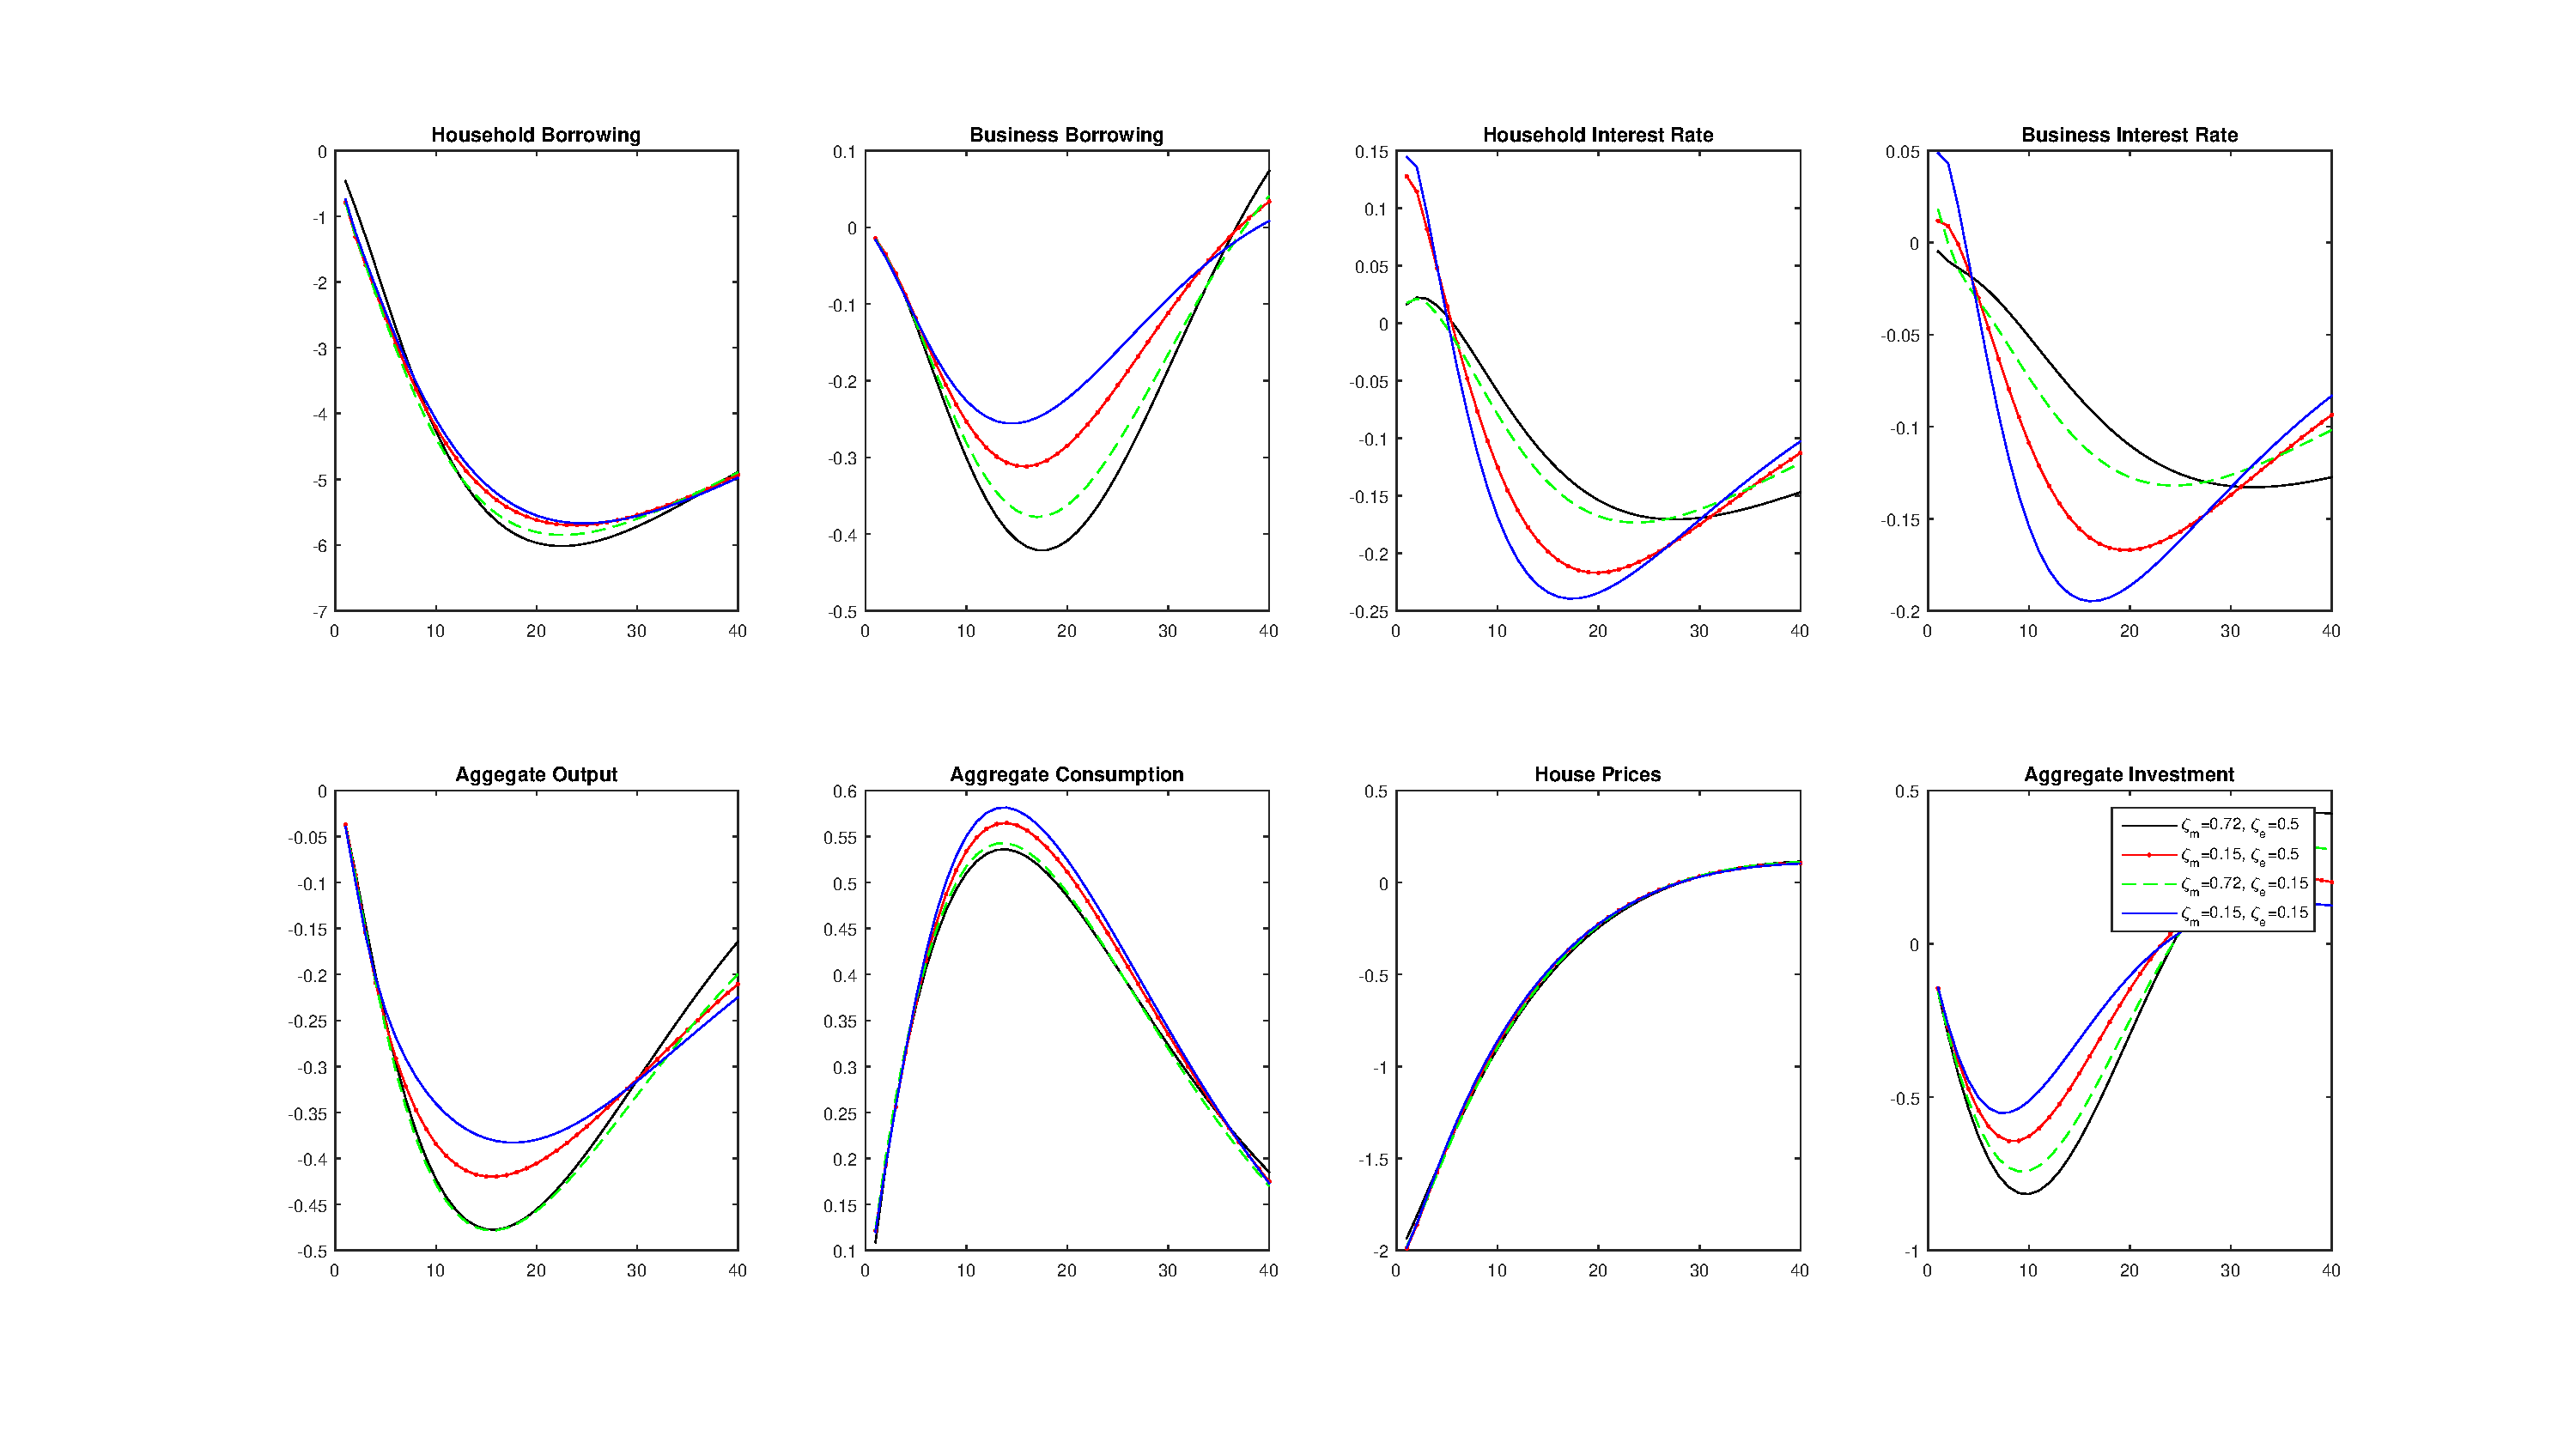
\includegraphics[scale=0.4]{stickinessNegativeShocksJ.pdf}
\end{figure}


Next we turn to Figure \ref{irf_stickiness_EbF}, which reports the effects of a negative capital price shock. Since the shock originates in the corporate sector, the immediate effects take place on the borrowing volume of businesses and aggregate investment: these variables decrease in all cases independent of the degree of stickiness. This effect spreads through two channels: first, the lower capital investment results in a substitution effect to housing investment, which pushes up the house prices. As a result, households shift some of their spending from housing to consumption in the short run, which results in a higher consumption and lower household borrowing. As a response to lower volume of household borrowing, and to prevent the substitution effect vfrom lower corporate rates, the bank cuts the housing lending rates. In the medium run after around 10 quarters, the effects of lower household lending rates start to kick and the households start shifting away from consumption back into housing. The largest fluctuations in household borrowing takes place when both interest rates are stickiest. Interestingly, the stickiness rate in mortgage lending again plays a more important role than corporate lending, even though the shock originates in the corporate sector. The overall effects on output are only marginally affected by interest rate stickiness in this case, since drop in investment is substantially larger than the short-term increases in consumption, which means the largest effect (through investment) does not transmit through interest rates. 



\begin{figure}[H]
\centering
\caption{Impulse responses to a negative expected capital price shock.}
\label{irf_stickiness_EbF}
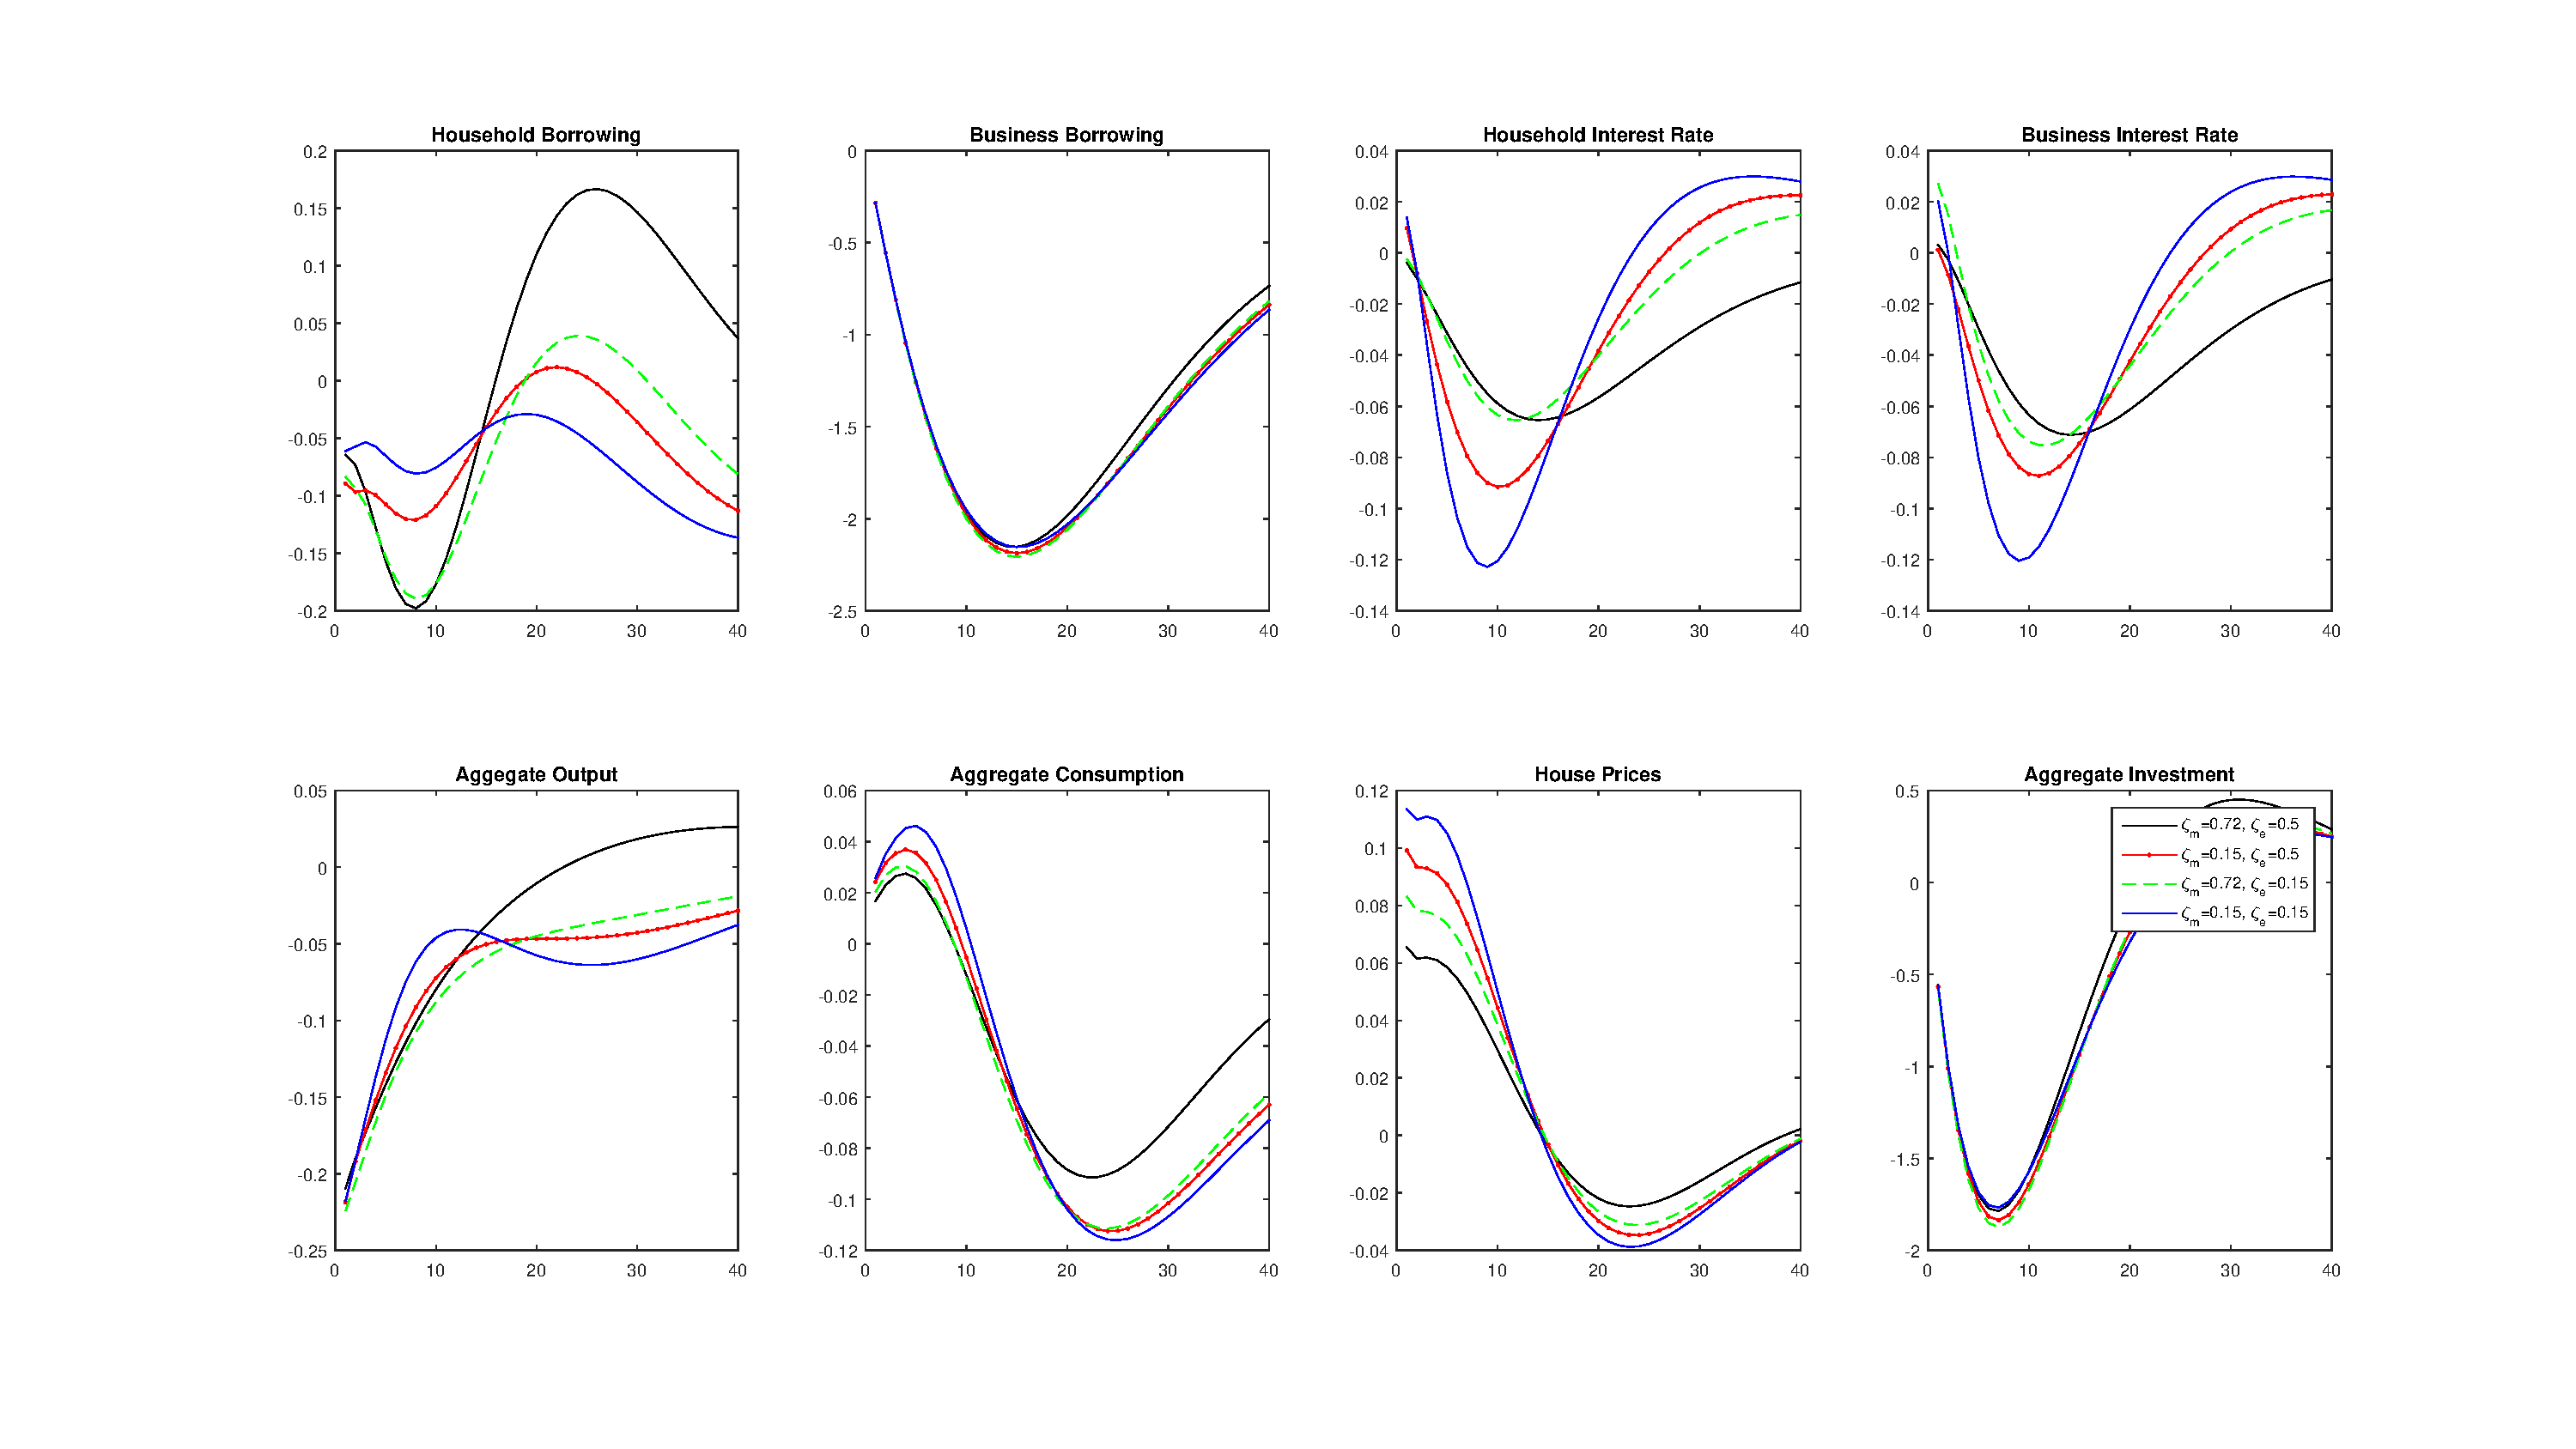
\includegraphics[scale=0.4]{stickinessNegativeShocksEbF.pdf}
\end{figure}


Finally we discuss the effects of negative bank capital shock, which is reported in Figure \ref{irf_stickiness_ECAB}. In this case the shock originates as a lower bank capital, to which the bank responds by increasing the lending rates in both sectors since it is not able to lend out as much. This unambiguously transmits through the rest of the economy in a negative manner, where the interest rates increase depending on the degree of stickiness (largest increase when stickiness is lowest). This results in lower borrowing volumes in both sectors. Investment and house prices both go down in response to the lower borrowing rates. In terms of consumption, there are again two effects: the lower household borrowing results in a substitution effect in households spending bundle, but at the same time the lower aggregate investment results in a lower household wealth. It is clear from the figure that the latter effect dominates and household consumption goes down, which also results in a lower aggregate output. Unlike the previous two cases, we see the largest effects on output when interest rate stickiness is lowest: in the previous cases, the bank reacts through interest rates by trying to mitigate the adverse effects of shocks in other sectors, hence the effects are strongest when interest rates are stickiest. In this case, the bank reacts by trying to shift the adverse effects on itself onto households and businesses, and therefore the effect tuns out strongest when interest rates are the least sticky. 



\begin{figure}[H]
\centering
\caption{Impulse responses to a negative bank capital shock.}
\label{irf_stickiness_ECAB}
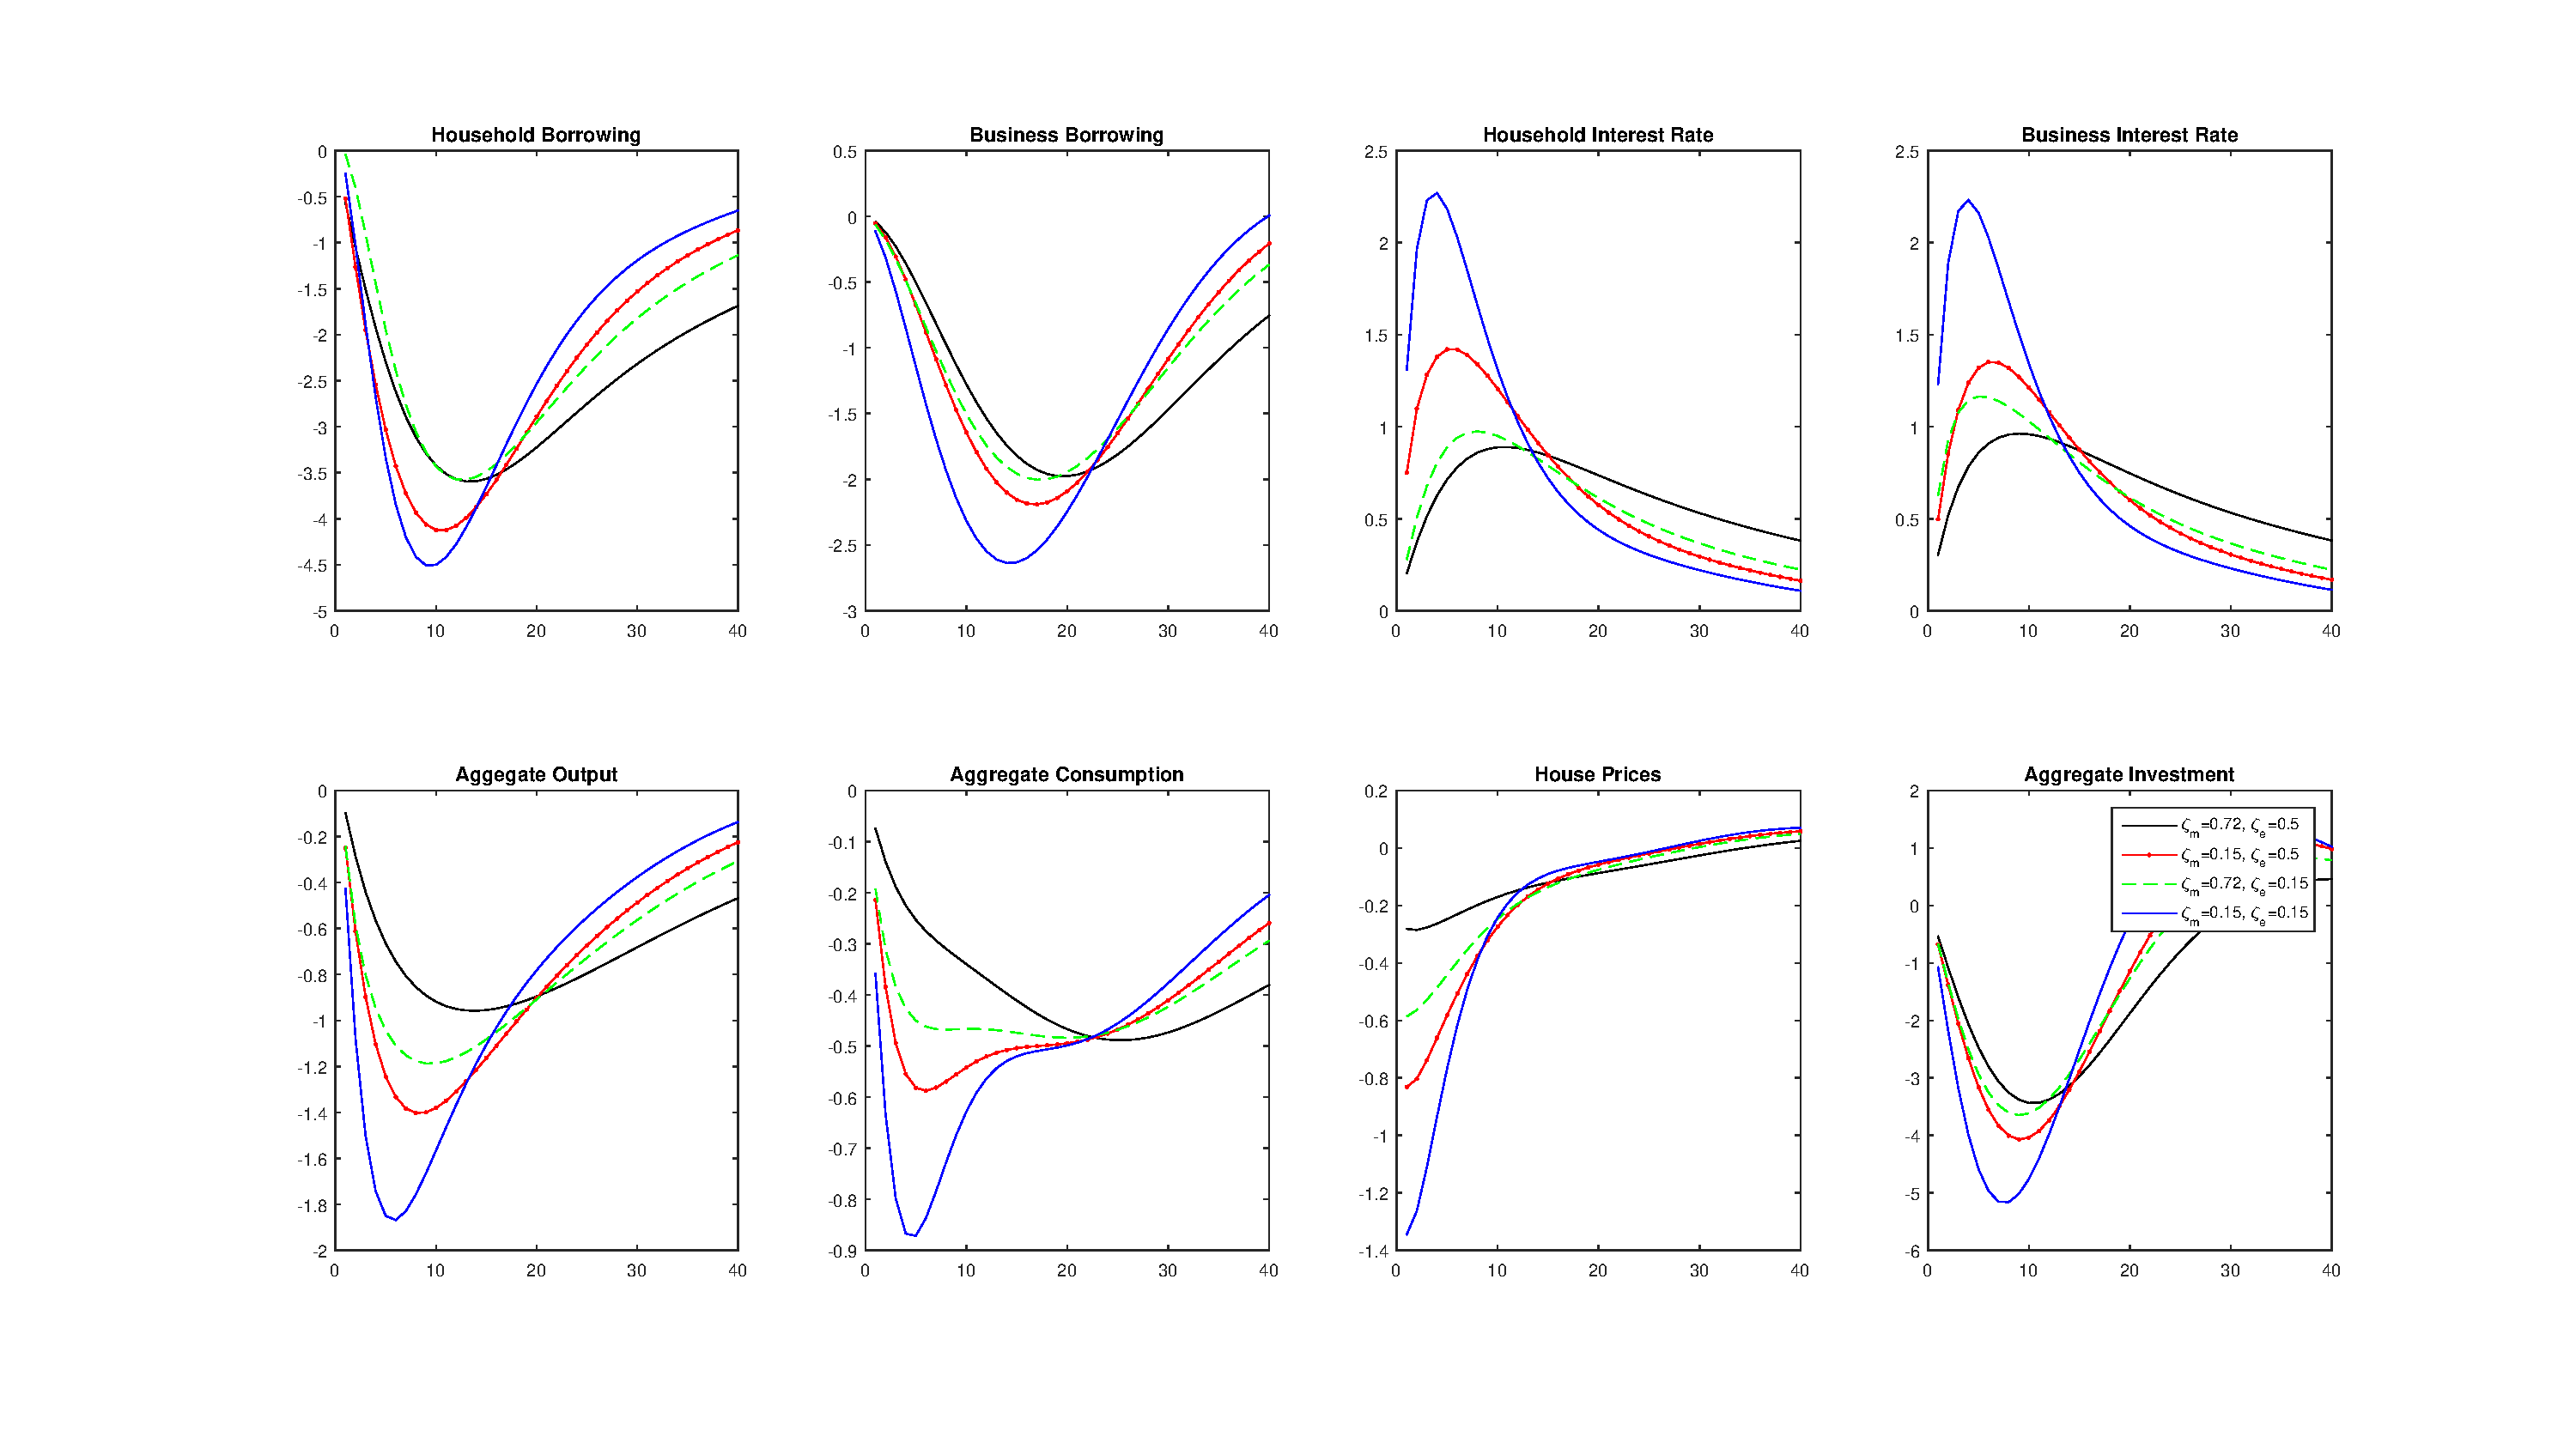
\includegraphics[scale=0.4]{stickinessNegativeShocksECAB.pdf}
\end{figure}




\subsection{Interest Rate Stickiness and Sectoral Capital Requirements}

Given the importance of interest rate stickiness on the transmission of shocks, in this section we analyze how interest rate stickiness affects the impact of macroprudential policies. We focus on the policies that transmit through interest rates in our model, namely sectoral capital requirements and sectoral countercyclical buffers\footnote{While the LTV limit also works through interest rates in reality, in our model it is a direct constraint on households and does not transmit through the bank and interest rates. Therefore we exclude this policy from our analysis in this section. A more realistic implementation of the LTV limit, along with loan-to-income ratios (LTI) is left to future research.}. In this case we focus on the response on lending volumes to a (positive) bank capital shock only, although the analysis can be extended to other shocks as well. 

Figures \ref{irf_stickiness_corpSCR} and \ref{irf_stickiness_housingSCR} report the effects of low (11 \%) and high (15 \%) SCRs on corporate and mortgage lending respectively. Two important observations stand out from the figures: first, increasing SCRs in either sector generally lowers the lending volume in both sectors. Second, the difference between impulse response under high and low SCRs is generally larger when interest rate stickiness is lower (i.e. the difference between green and blue curves tends to be larger than the difference between red and black curves). This suggests that a high degree of interest rate stickiness may weaken the effect of minimum capital requirements. 

Similarly, Figures \ref{irf_stickiness_corporateCCyB} and \ref{irf_stickiness_housingCCyB} report the effects of no sectoral CCyB and a 2.5 \% sectoral CCyB on housing and corporate lending respectively\footnote{Similar to the previous section, the 2.5 \% CCyB is obtained by tuning the parameter in reaction functions to generate a standard deviation of 2.5 \% in the capital requirement rates.}. We observe in this case that, in both sectors, introducing a sectoral CCyB lowers the lending volume in that sector. However, there are two important differences compared to the SCRs: first, the differences with and without interest rate stickiness are smaller compared to the SCRs. Second, unlike the SCRs, we observe a substitution effect towards the other sector in this case: a sectoral CCyB in corporate lending increases the volumne of mortgage lending, and similarly a sectoral CCyB in mortgage lending increases the volume of corporate lending. These results emerge due to the gradual nature of CCyBs: since the tool builds up slowly over time, interest rate stickiness has a much smaller impact and the graduality allows the bank some time to substitute its lending volume towards the other sector. 

Overall, these results suggest that interest rate stickiness plays an important role both in terms of the transmission of shocks through the economy, and also in terms of the effectiveness of macroprudential tools that work through interest rates. This presents a new, important channel for the design of macroprudential policies and particularly for tools that affect the degree of interest rate stickiness through long-term contracts. 



\begin{figure}[H]
\centering
\caption{The impact of corporate SCR on lending volumes with high and low levels of interest rate stickiness. }
%Cumulative differences are 3.63 \% and 2. 93 \% for mortgage and corporate lending respectively. }
\label{irf_stickiness_corpSCR}
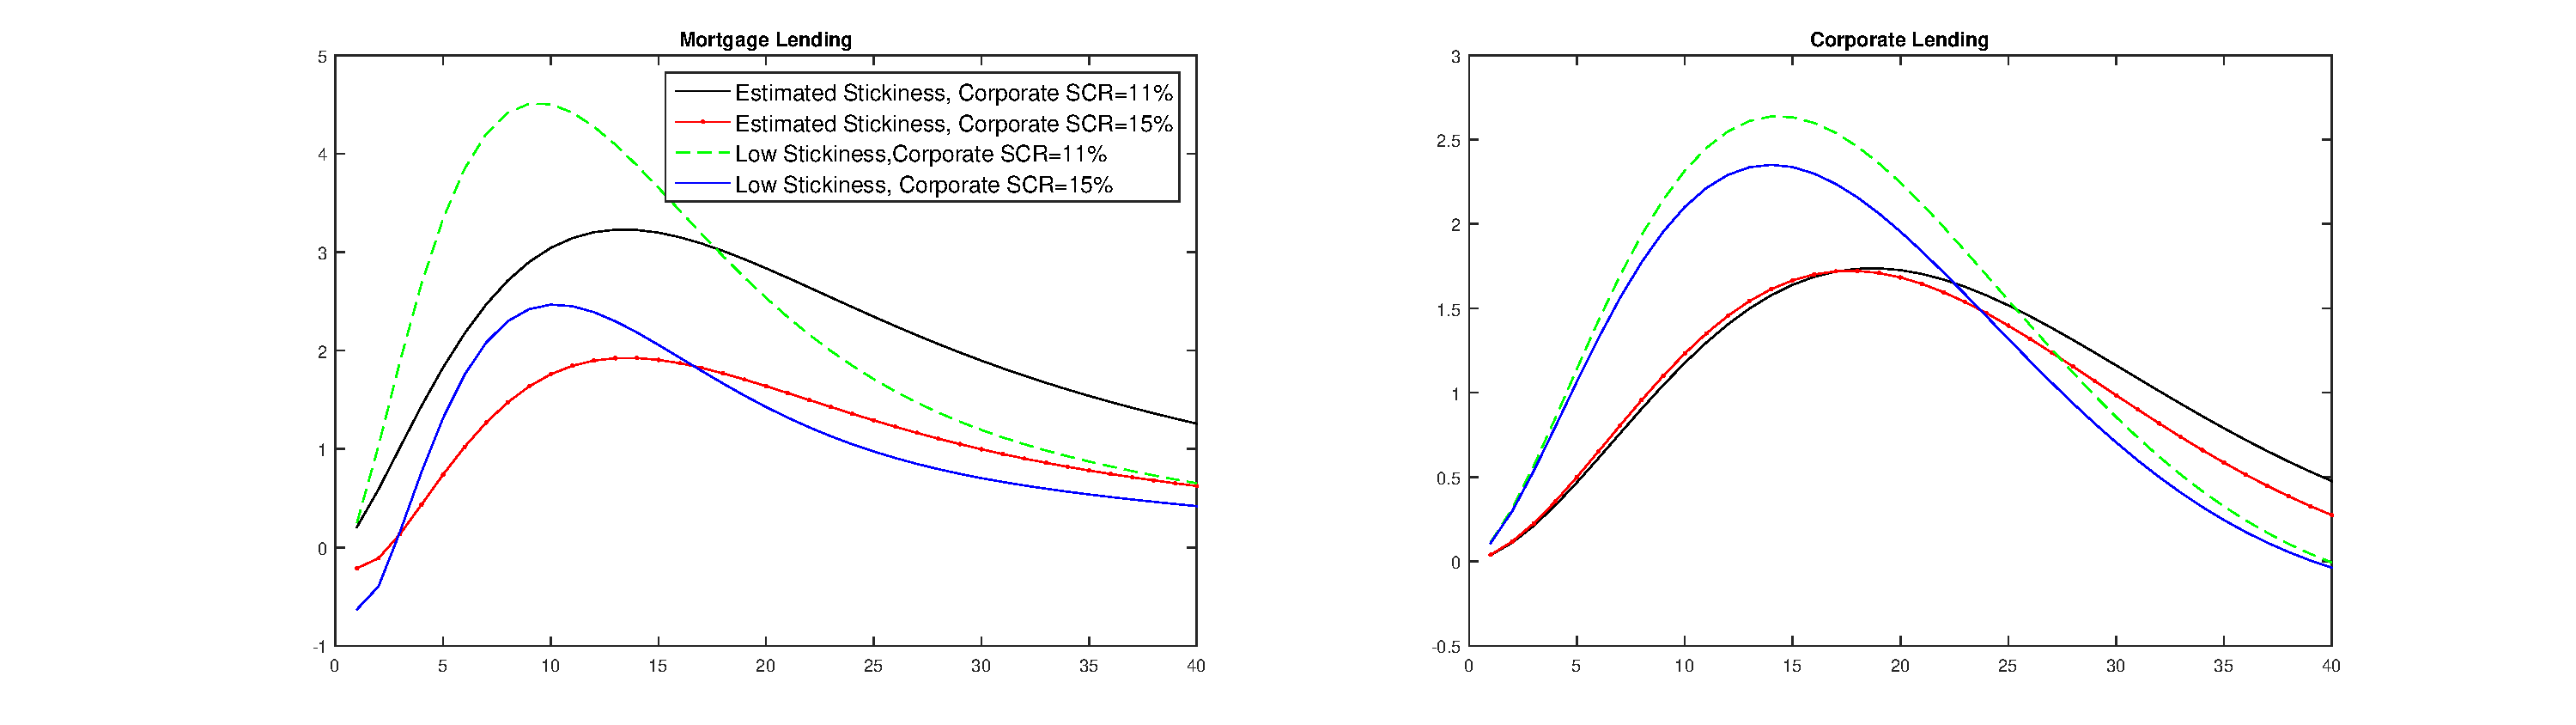
\includegraphics[scale=0.35]{stickiness_corporate_SCRECAB.pdf}
\end{figure}

\begin{figure}[H]{}
\centering
\caption{The impact of housing SCR on lending volumes with high and low levels of interest rate stickiness.}
% Cumulative differences are 5.12 \% and 3.57 \% for mortgage and corporate lending respectively. }
\label{irf_stickiness_housingSCR}
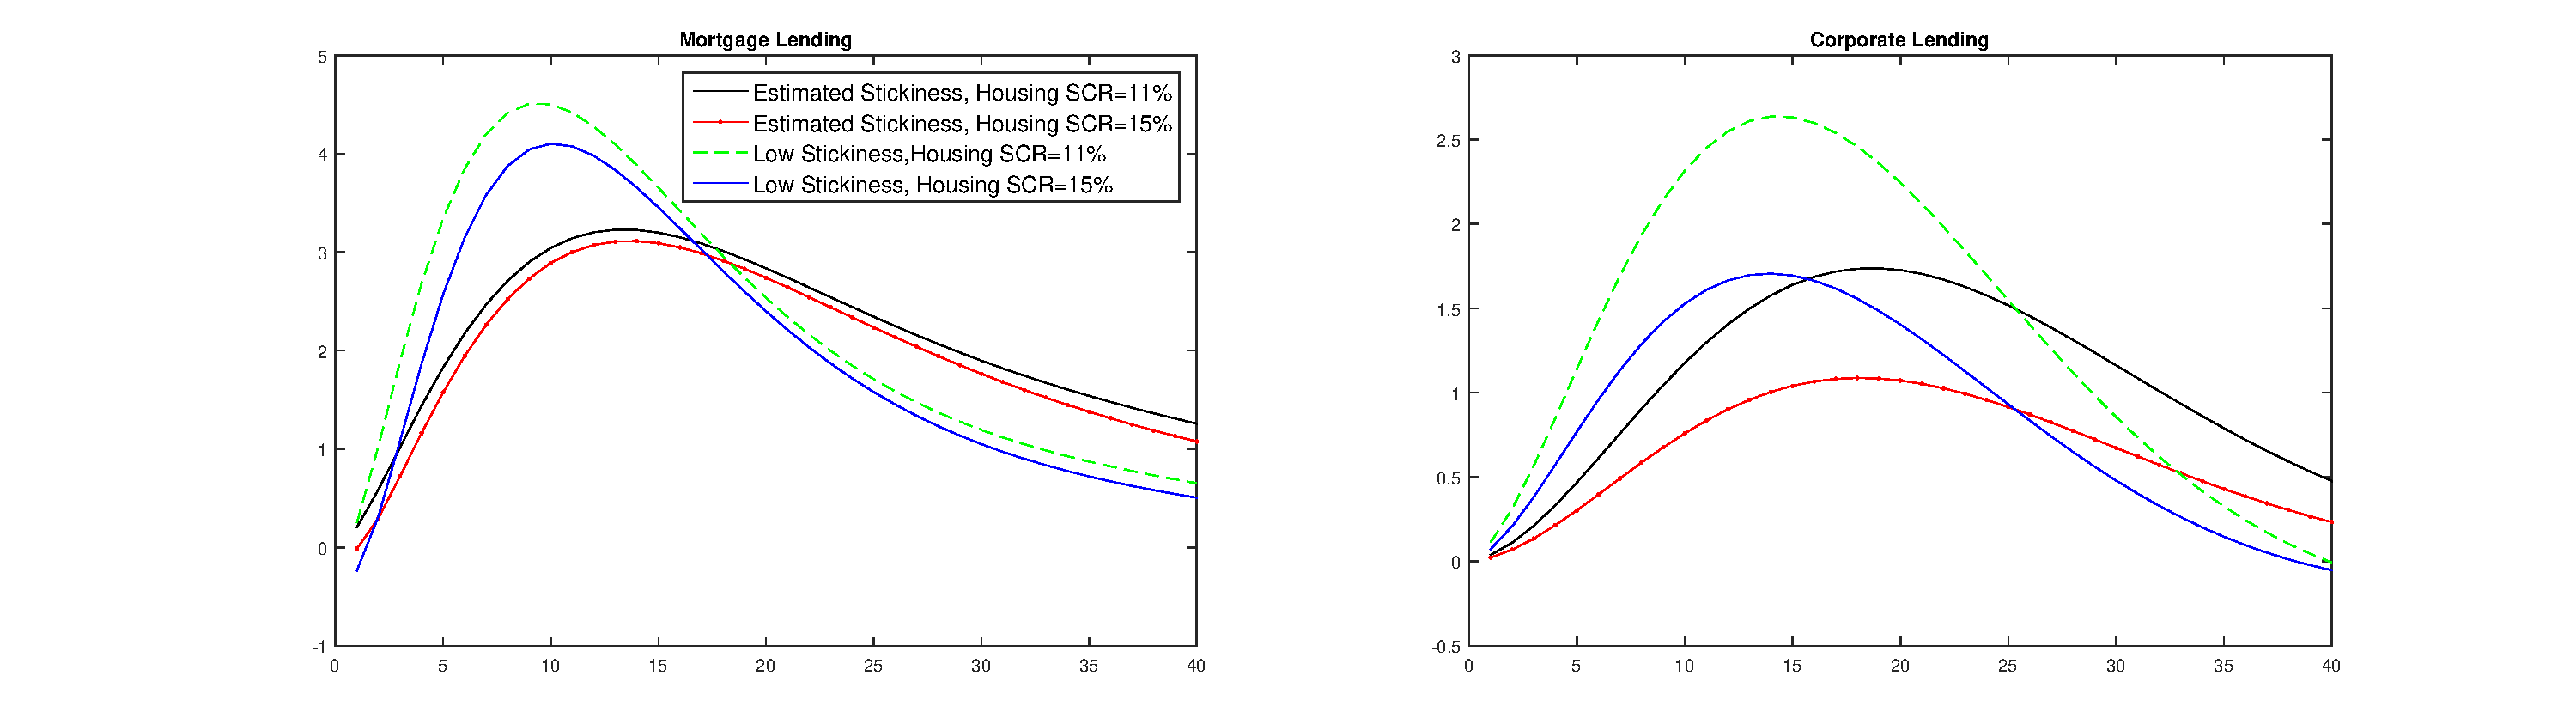
\includegraphics[scale=0.35]{stickiness_housing_SCRECAB.pdf}
\end{figure}


\begin{figure}[H]
\centering
\caption{The impact of a 2.5 \% corporate CCyB on lending volumes with high and low levels of interest rate stickiness. }
% Cumulative differences are -4.07 \% and 0.09 \% for mortgage and corporate lending respectively. }
\label{irf_stickiness_corporateCCyB}
\includegraphics[scale=0.35]{stickiness_corporate_ccybECAB.pdf}
\end{figure}

\begin{figure}[H]
\centering
\caption{The impact of a 2.5 \% housing CCyB on lending volumes with high and low levels of interest rate stickiness.}
% Cumulative differences are -0.09 and 0.14 \% for mortgage and corporate lending respectively. } 
\label{irf_stickiness_housingCCyB}
\includegraphics[scale=0.35]{stickiness_housing_ccybECAB.pdf}
\end{figure}


\begin{comment}
\begin{figure}[H]
\caption{Positive housing preference shock. We calculate the cumulative difference is calculated as follows: we first calculate the area between impulse responses with and without interest rate stickiness. The cumulative difference is then given as the difference between these two areas. }
\subfigure[Cumulative differences: 0.45 \% and -0.21 \%.]{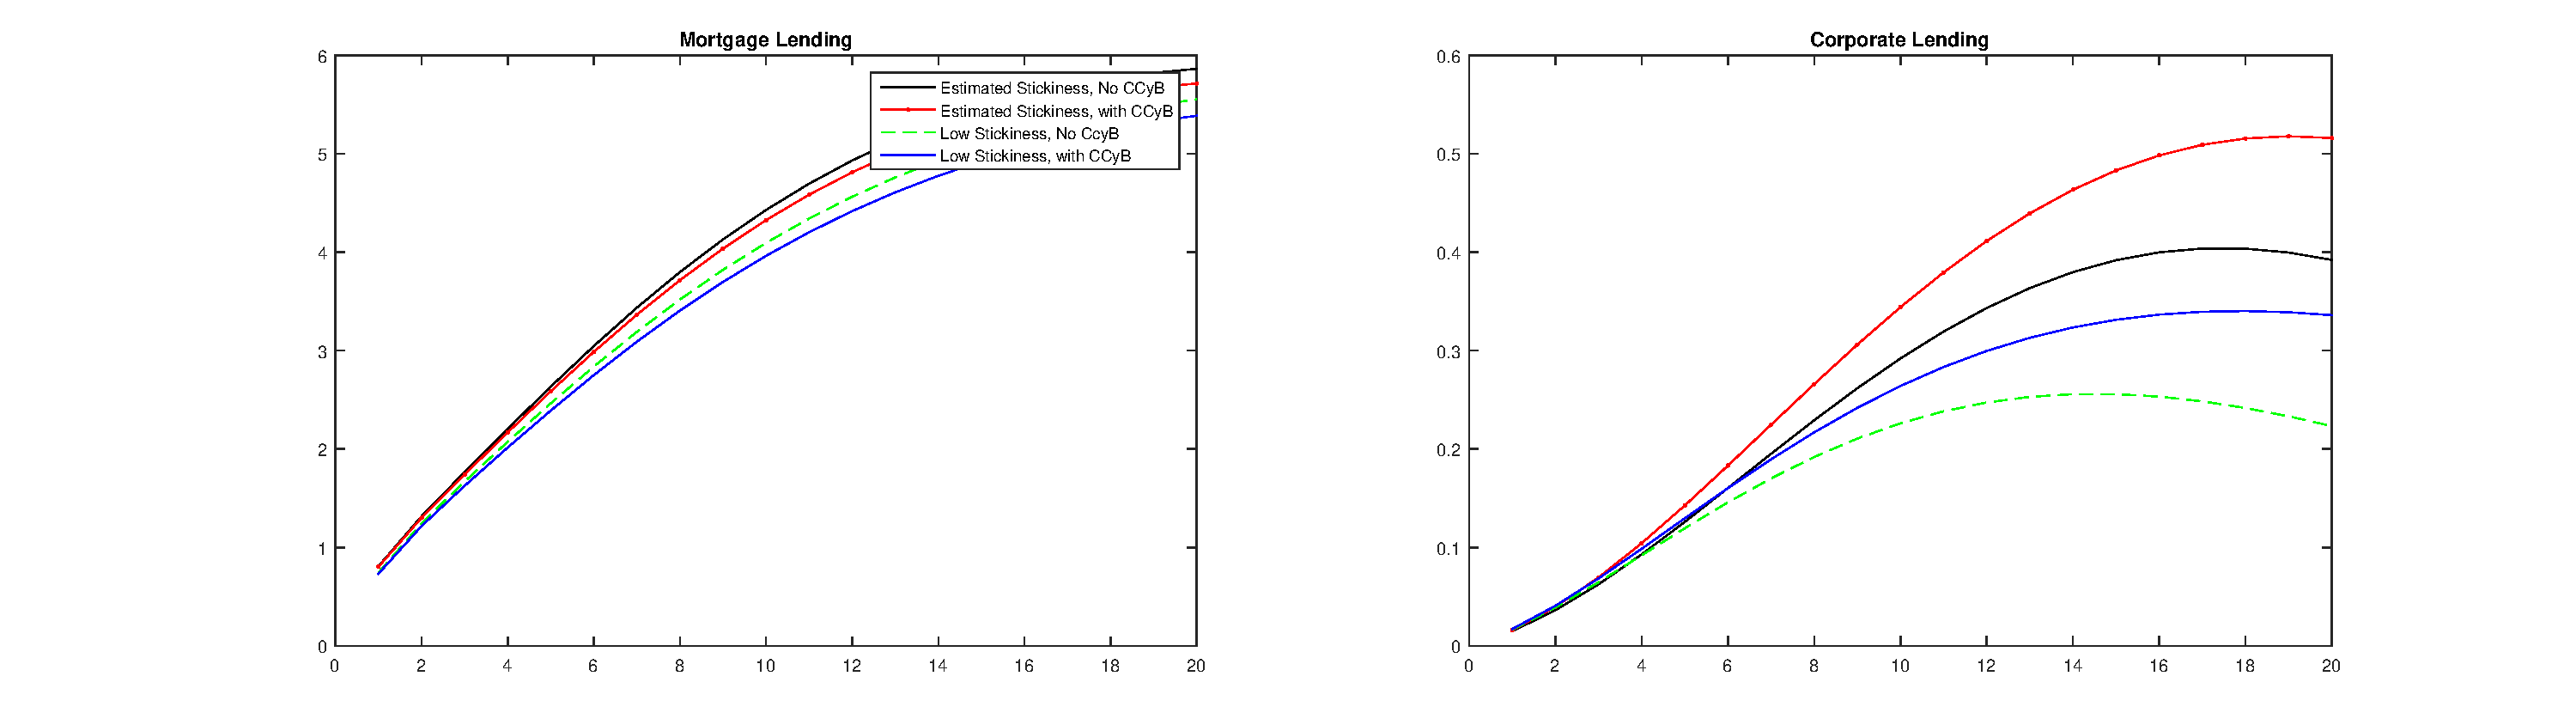
\includegraphics[scale=0.35]{stickiness_ccybJ.pdf}}
\subfigure[Cumulative differences: -1.18 \% and 0.25 \%.]{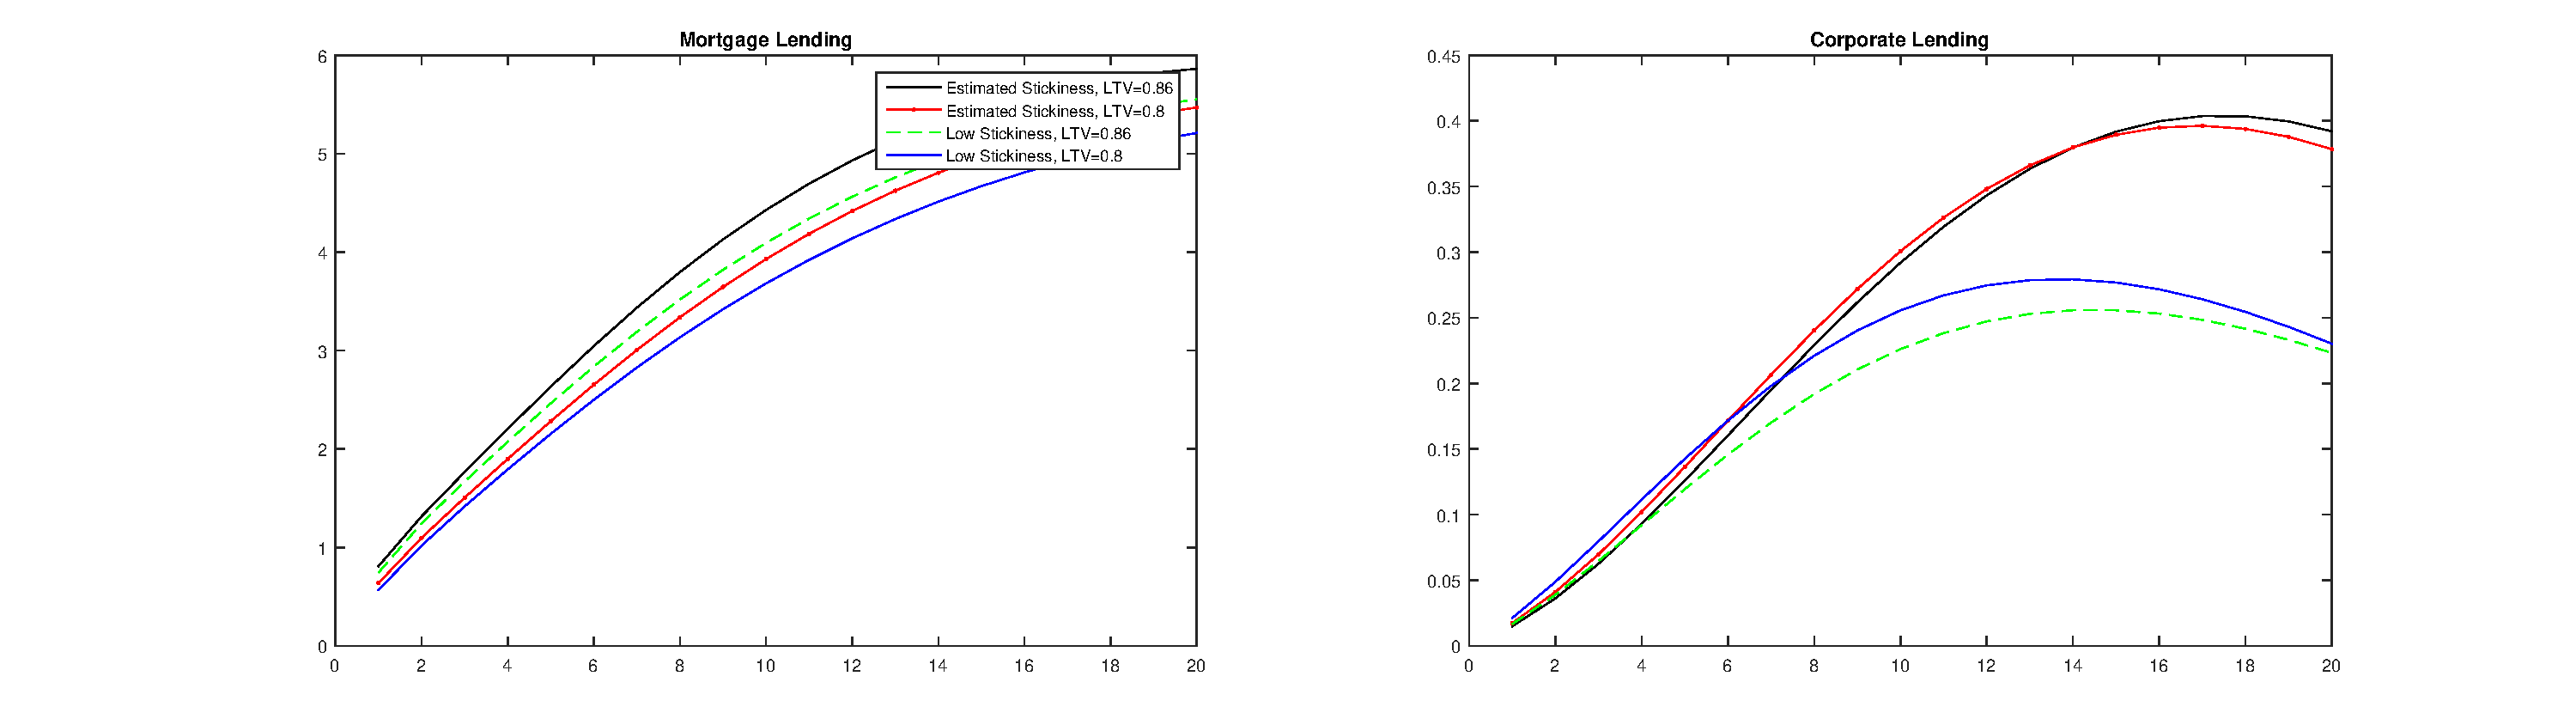
\includegraphics[scale=0.35]{stickiness_LTVJ.pdf}}
\subfigure[Cumulative differences: 2.85 \% and 0.91 \%.]{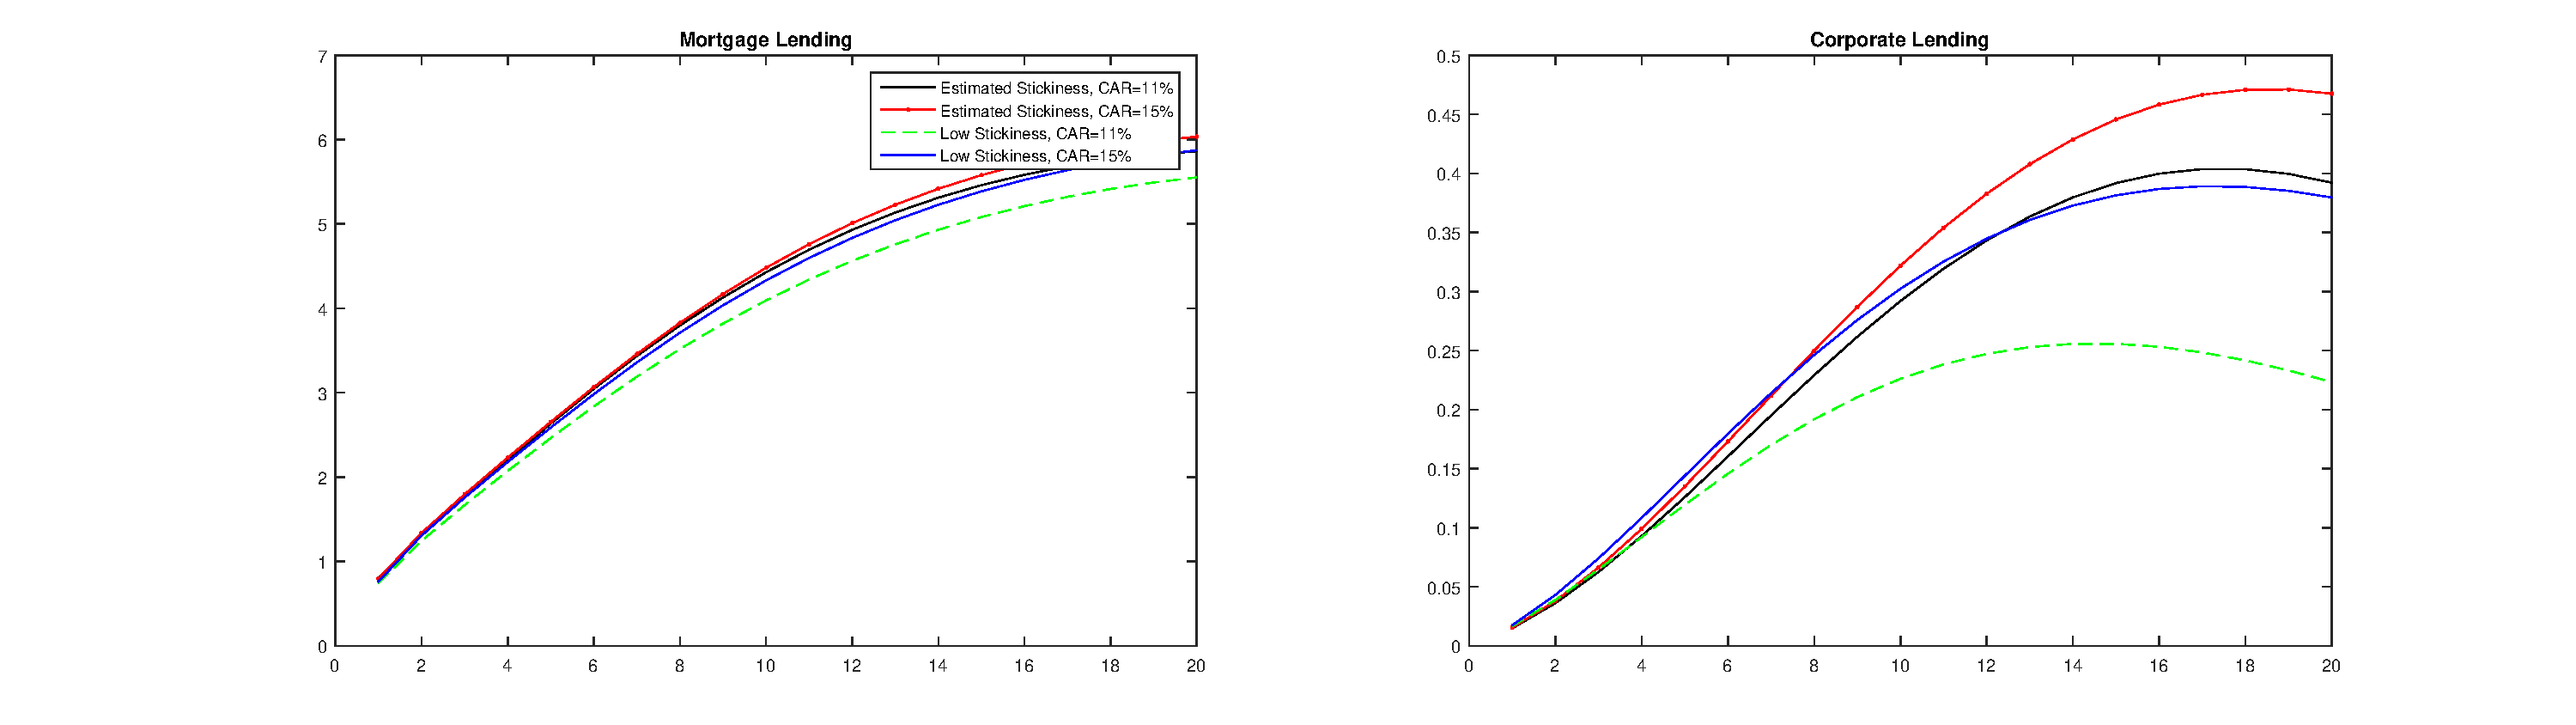
\includegraphics[scale=0.35]{stickiness_CARJ.pdf}}
\end{figure}

\begin{figure}[H]
\caption{Positive expected capital shock. Cumulative difference calculated as the  }
\subfigure[Cumulative differences: 1.4 \% and -0.34 \%.]{\includegraphics[scale=0.35]{stickiness_ccybEbF.pdf}}
\subfigure[Cumulative differences: -0.02 \% and 0.003 \%.]{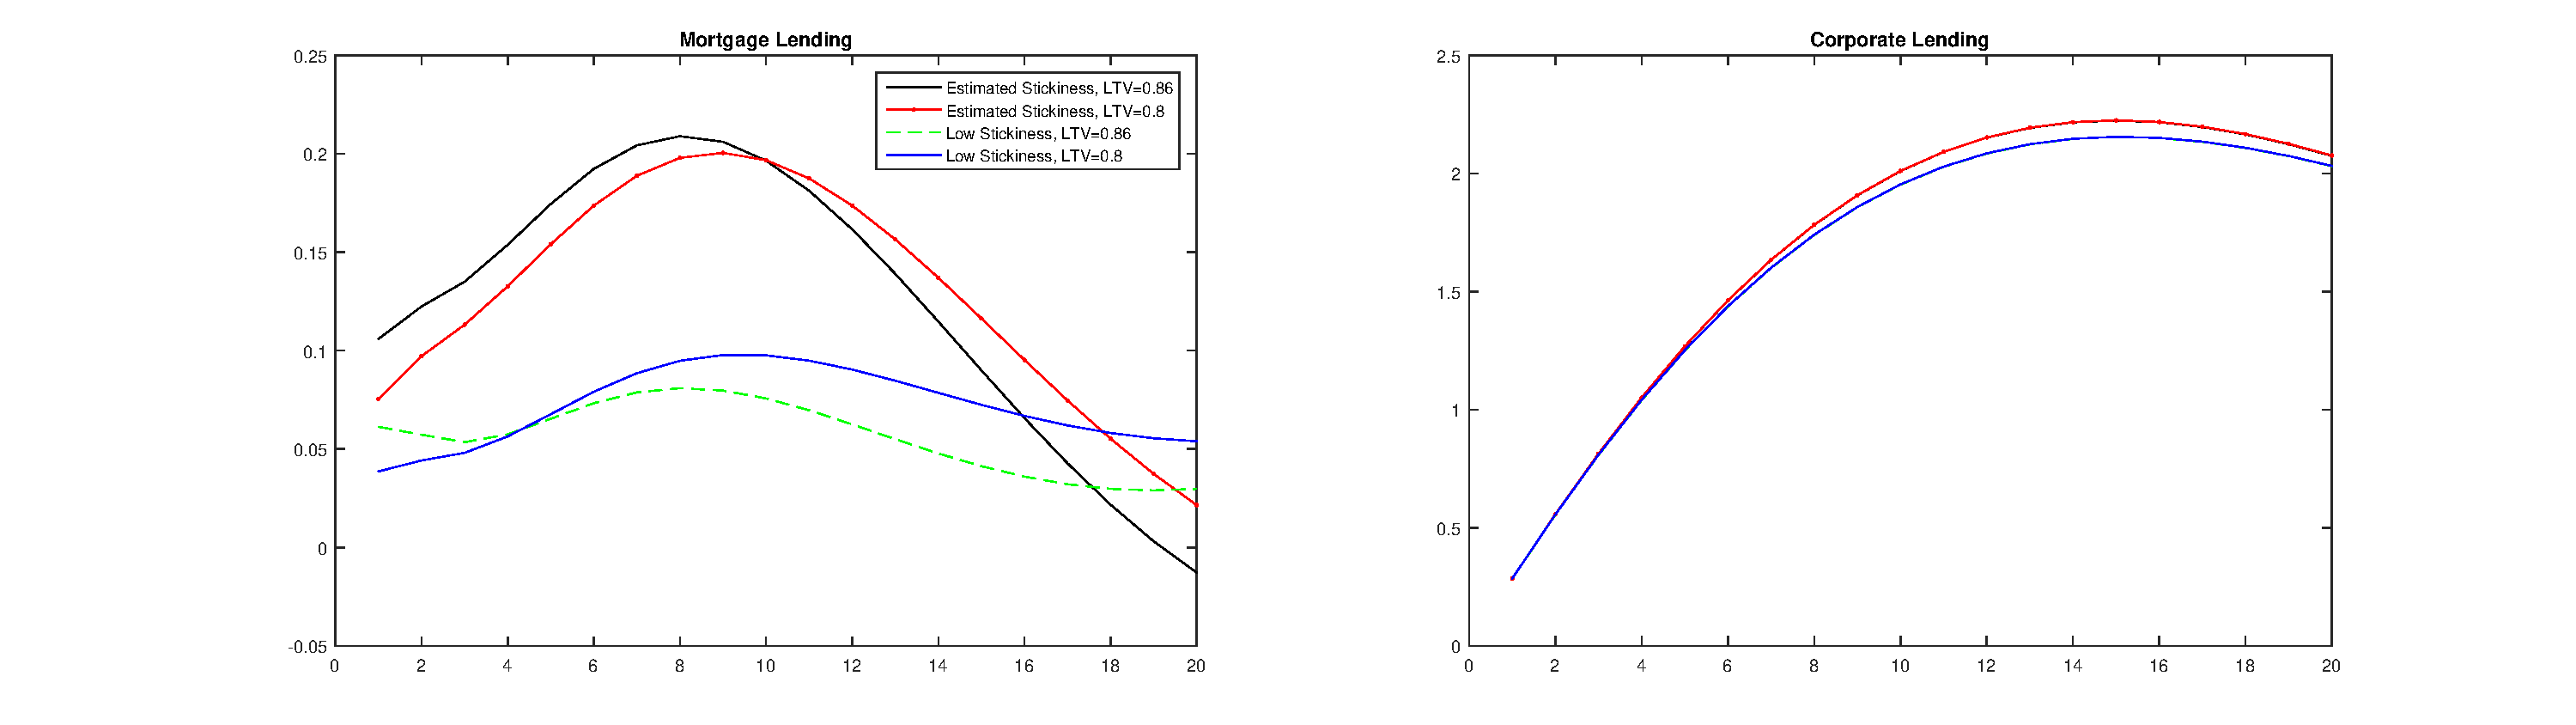
\includegraphics[scale=0.35]{stickiness_LTVEbF.pdf}}
\subfigure[Cumulative differences: 0.85 \% and 0.34 \%.]{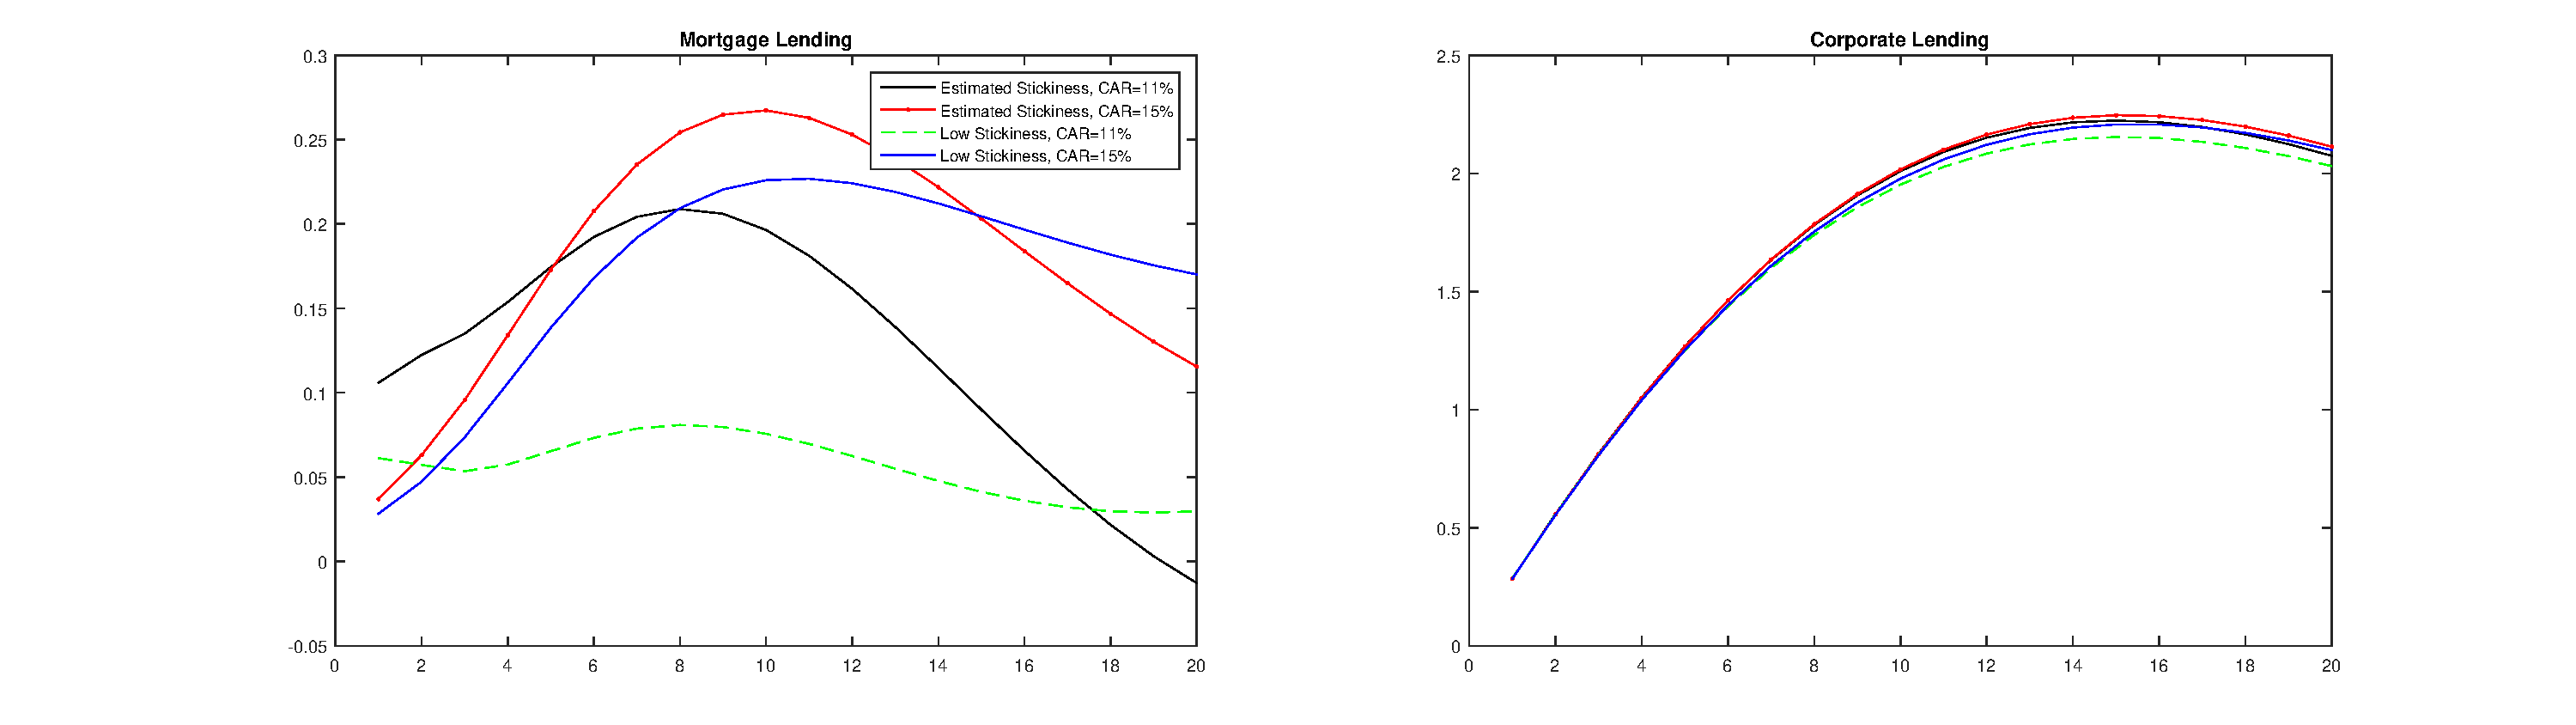
\includegraphics[scale=0.35]{stickiness_CAREbF.pdf}}
\end{figure}



\begin{figure}[H]
\caption{Positive bank capital shock.}
\subfigure[Cumulative differences: 2.2 \% and 0.128 \%.]{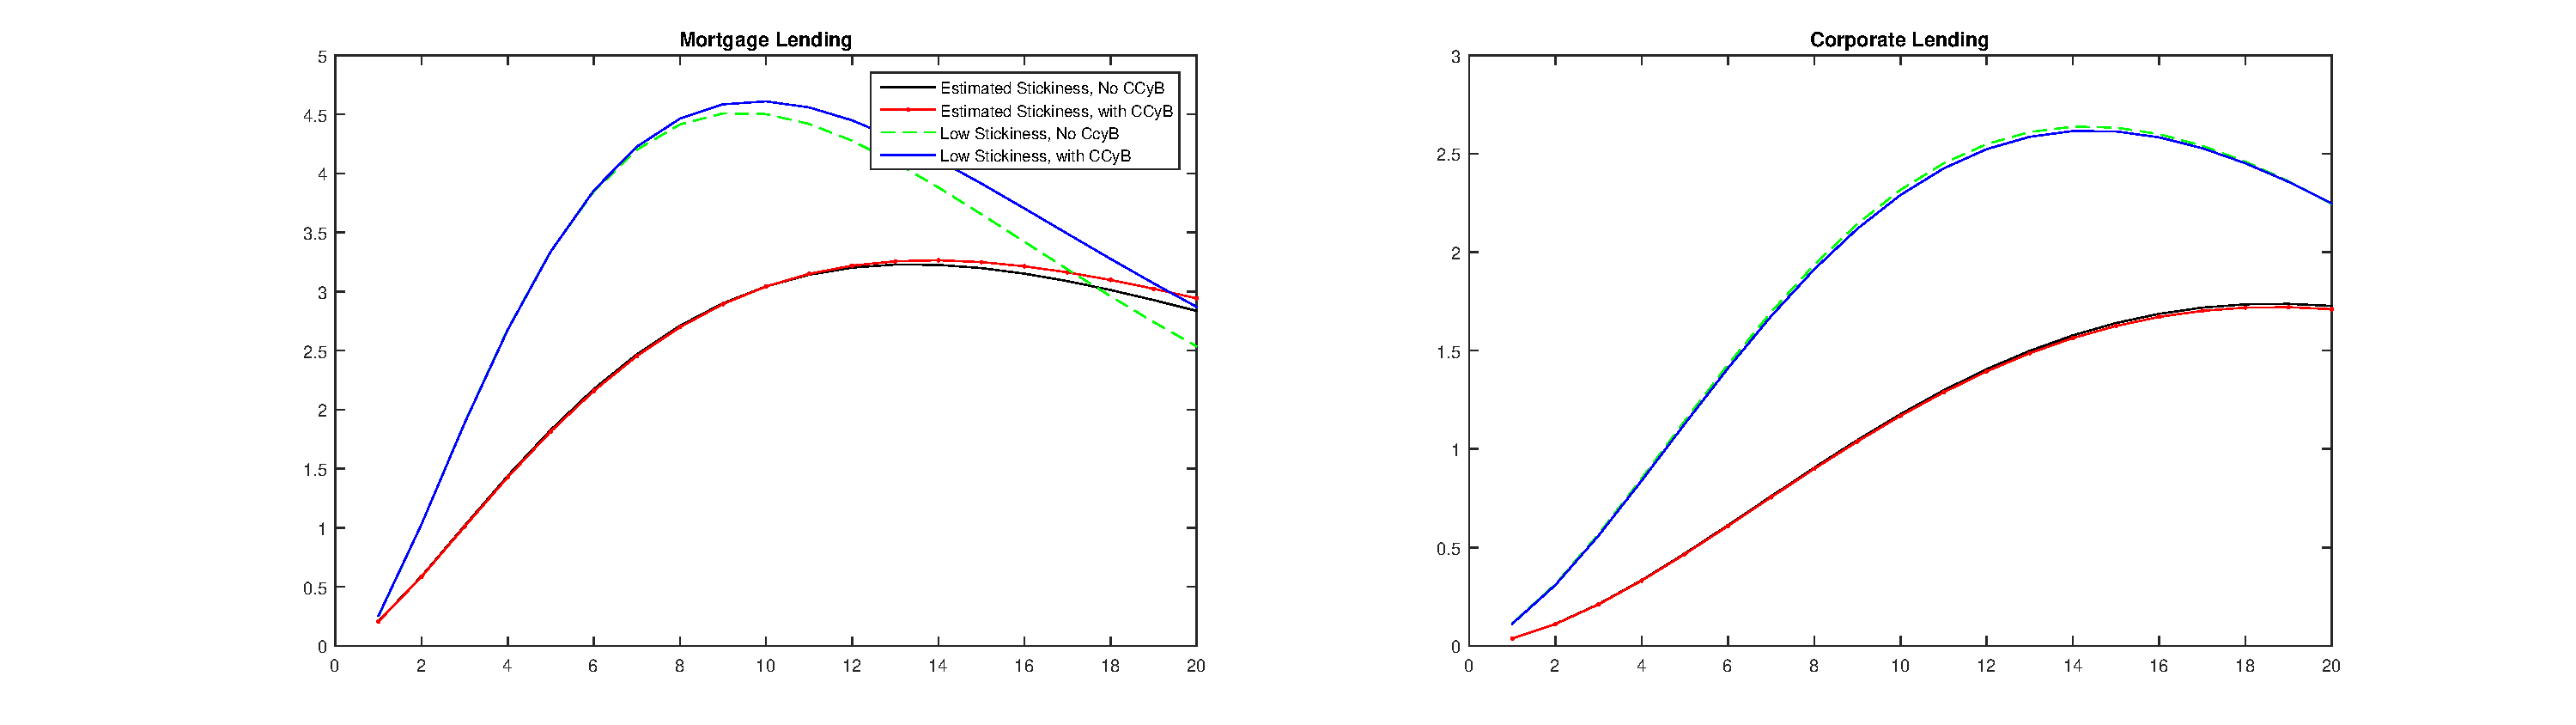
\includegraphics[scale=0.35]{stickiness_ccybECAB.pdf}}
\subfigure[Cumulative differences: 3.62 \% and 0.33 \%.]{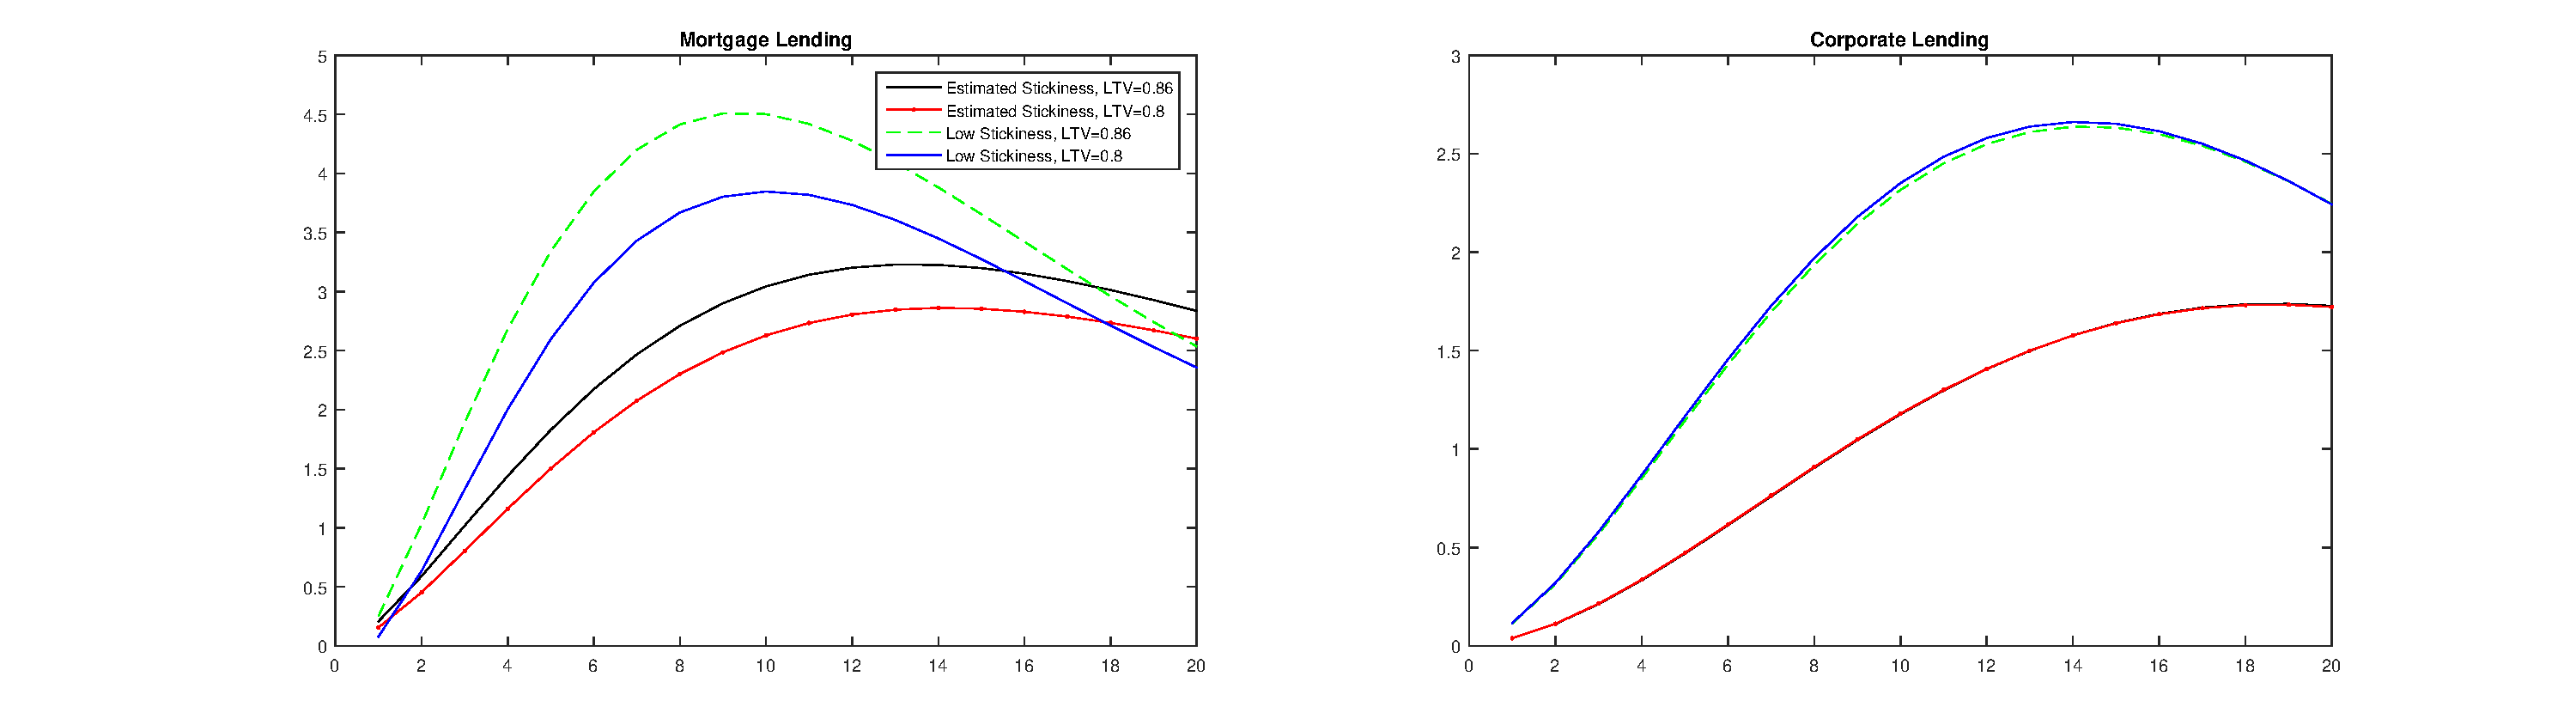
\includegraphics[scale=0.35]{stickiness_LTVECAB.pdf}}
\subfigure[Cumulative differences: 11.59 \% and 6.25 \%.]{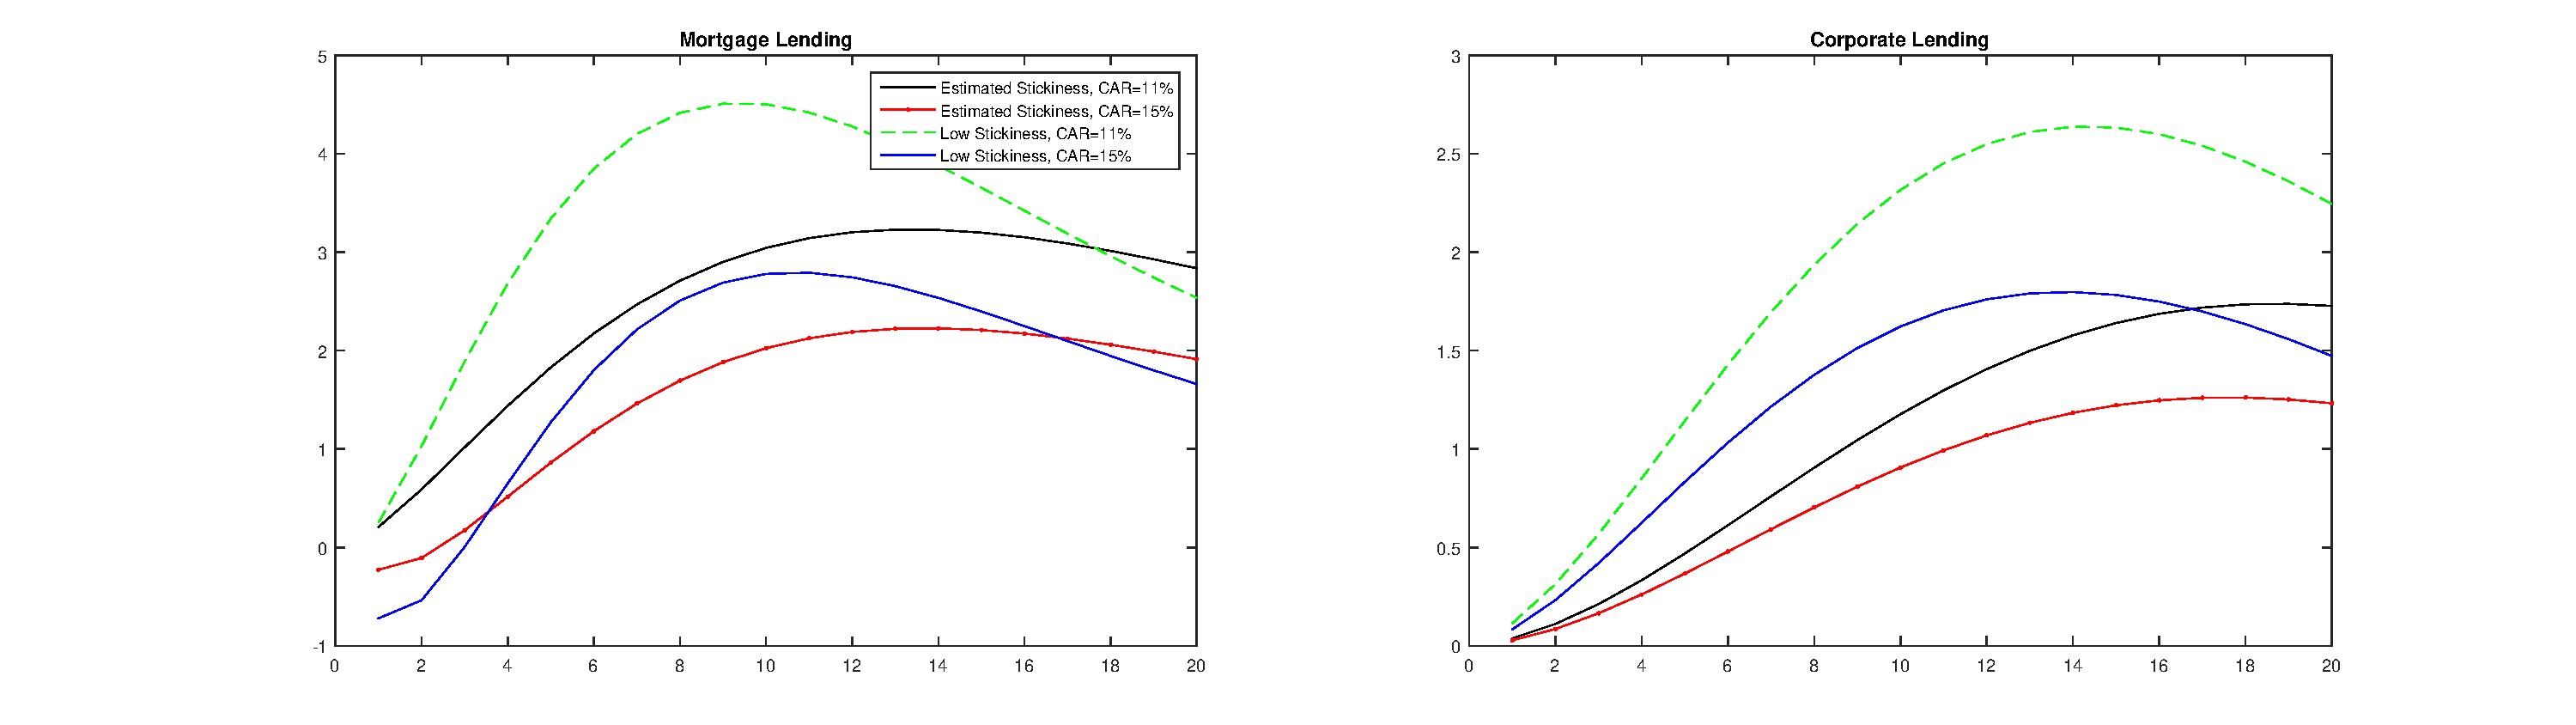
\includegraphics[scale=0.35]{stickiness_CARECAB.pdf}}
\end{figure}



\end{comment}



\section{Conclusion (old version)}

In this paper, we provide cross country evidence of interest rate sluggishness due to fixed interest rate loan contract. The response of fixed term interest rates is lower as compared to the floating interest rate term. Moreover,the immediate impact on lending rates is small even for floating interest loans. The interest rate pass through is complete for the floating rate loans and incomplete for fixed term interest loans, both for the UK as well as the four Euro zone economies.


We use a two sector DSGE model with a crucial role for the banking sector,  to 1)evaluate the role of interest rate stickiness in the transmission of macro prudential policy and 2) study the interaction between capital requirement and the LTV limit. We find that sluggishness in the adjustment of interest rates lowers the impact of the capital regulation on the economy.At the same, interest rate stickiness makes the a change in LTV policy more effective. It also increases the volatility of macro economic variables to various shocks. We find that interest rate stickiness dampens the effectiveness of the countercyclical capital policy under different shocks. However countercyclical capital rule is still more effective than the LTV rule.As regards the interaction between the policy tools, we find that the impact of a change in capital requirement is higher when the LTV limit in the economy is high. On the other hand, the change in LTV limit has a higher impact when the capital requirement is lower.















\section{References}

\hspace*{0.6cm}

Aikman, D., Bridges, J., Kashyap, A. and Siegert, C., 2019. Would macroprudential regulation have prevented the last crisis?. Journal of Economic Perspectives, 33(1), pp.107-30. \\

Aikman, D., Giese, J., Kapadia, S. and McLeay, M., 2019. Targeting financial stability: macroprudential or monetary policy?. \\

Andries N. and Billon S.2014.'Retail bank interest rate pass-through in the Euro area: An empirical survey'.Economic Systems 40 (2016) 170–194.\\

Benes, J., and M. Kumhof. 2011. 'Risky Bank Lending and Optimal
Capital Adequacy Regulation.' IMF Working Paper No. 11/130.\\


Bernanke, B. S., M. Gertler, and S. Gilchrist. 1999, 'The financial accelerator in a quantitative business cycle framework'. Handbook of Macroeconomics, Elsevier.\\

Berstein S., and R. Fuentes, 2002, "From Policy Rate to Bank Lending Rates: the Chilean Banking Industry," Paper presented at the Sixth Annual Conference of the Central Bank of Chile, December.\\

Bianchi, J.: 2011, 'Overborrowing and Systemic Externalities in the Business Cycle'.
American Economic Review 101(7), 3400 -3426.\\

Bianchi, J. and Mendoza, E.G., 2010. Overborrowing, financial crises and'macro-prudential'taxes (No. w16091). National Bureau of Economic Research. \\

Bluwstein K., Brzoza-Brzezina M., Gelain P.and Kolasa M.2018, 'Multi-period loans, occasionally binding constraints and monetary policy:
a quantitative evaluation'.Bank of England Staff Working paper no.749.\\

Bonciani, D. and Van Roye, B., 2016. Uncertainty shocks, banking frictions and economic activity. Journal of Economic Dynamics and Control, 73, pp.200-219. \\

Burgess, S., Fernandez-Corugedo, E., Groth, C., Harrison, R., Monti, F., Theodoridis, K. and Waldron, M., 2013. The Bank of England’s forecasting platform: COMPASS, MAPS, EASE and the suite of models. documento de trabajo, (471).

Calvo, G. A.: 1983, 'Staggered prices in a utility-maximizing framework'. Journal of Monetary Economics 12(3), 383-398.\\

Campbell, J. Y. and J. F. Cocco: 2015, 'A Model of Mortgage Default'. The Journal of Finance 70(4), 1495-1554.\\

Christiano, L. J., R. Motto, and M. Rostagno: 2014, 'Risk Shocks'. American
Economic Review 104(1), 27-65.\\

Clerc, L., A. Derviz, C. Mendicino, S. Moyen, K. Nikolov, L. Stracca, J. Suarez,
and A. P. Vardoulakis: 2015, 'Capital Regulation in a Macroeconomic Model with
Three Layers of Default'. International Journal of Central Banking 11(3), 9-63.\\

Collard, F., Dellas, H., Diba, B. and Loisel, O., 2017. Optimal monetary and prudential policies. American Economic Journal: Macroeconomics, 9(1), pp.40-87. \\

Ferreira, L.N. and Nakane, M.I., 2015. Macroprudential Policy in a DSGE Model: anchoring the countercyclical capital buffer. FEA/USP. \\

Financial Policy Committee, 2016. The Financial Policy Committee’s approach to setting the countercyclical capital buffer. London: Bank of England. \\

Forlati, C. and L. Lambertini: 2011, 'Risky Mortgages in a DSGE Model'. Interna-
tional Journal of Central Banking 7(1), 285-335.\\

Galati, G. and Moessner, R., 2018. What do we know about the effects of macroprudential policy?. Economica, 85(340), pp.735-770.\\

Gambacorta, L. and Karmakar, S., 2016. Leverage and risk weighted capital requirements.\\

Gelain, P. and Ilbas, P., 2017. Monetary and macroprudential policies in an estimated model with financial intermediation. Journal of Economic Dynamics and Control, 78, pp.164-189.\\

Gerali, A., S. Neri, L. Sessa, and F. M. Signoretti: 2010, 'Credit and Banking in
a DSGE Model of the Euro Area'. Journal of Money, Credit and Banking 42,
107-141.\\

Goodhart, C. A. E., A. K. Kashyap, D. P. Tsomocos, and A. P. Vardoulakis: 2013,
'An Integrated Framework for Analyzing Multiple Financial Regulations'. Inter-
national Journal of Central Banking 9(1), 109-144.\\

 Hodbod A.,  Huber S. and Vasilev K.2016 'Sectoral Risk Weights and Macroprudential Policy'. Working paper.\\
 
Iacoviello, M.: 2005, 'House Prices, Borrowing Constraints, and Monetary Policy in
the Business Cycle'. American Economic Review 95(3), 739-764.\\

Ingholt, M.M., 2019. Multiple credit constraints and time-varying macroeconomic dynamics (No. 137). Danmarks Nationalbank Working Papers.\\



Jeanne, O. and A. Korinek: 2010, 'Excessive Volatility in Capital Flows: A Pigouvian
Taxation Approach'. American Economic Review 100(2), 403-407.\\

Kahou, M.E. and Lehar, A., 2017. Macroprudential policy: A review. Journal of financial stability, 29, pp.92-105.\\

Karmakar, S., 2016. Macroprudential regulation and macroeconomic activity. Journal of financial stability, 25, pp.166-178.\\

Kiyotaki, N. and J. Moore: 1997, 'Credit Cycles'. Journal of Political Economy
105(2), 211-248.\\

Kobayashi, T. 2008. “Incomplete Interest Rate Pass-Through and
Optimal Monetary Policy.” International Journal of Central
Banking 4 (3): 77–118.\\




Lowe, P. and T. Rohling (1992), ‘Loan Rate Stickiness: Theory and Evidence’, Research Discussion Paper No. 9206, Reserve Bank of Australia.\\

Martinez-Miera, D., and J. Suarez. 2012. 'A Macroeconomic Model
of Endogenous Systemic Risk Taking.' CEPR Discussion Paper
No. 9134.\\

Meh, C., and K. Moran. 2010. 'The Role of Bank Capital in the
Propagation of Shocks.' Journal of Economic Dynamics and
Control 34 (3), 555–76.\\

Mendicino, C., Nikolov, K., Suarez, J. and Supera, D., 2018. Optimal dynamic capital requirements. Journal of Money, Credit and Banking, 50(6), pp.1271-1297.\\

Moazzami, B., 1999. 'Lending rate stickiness and monetary transmission mechanism: the case of Canada and the United States'.
Applied Financial Economics 9, 533–538.\\


Nier, E. and Baumann, U., 2006. Market discipline, disclosure and moral hazard in banking. Journal of Financial Intermediation, 15(3), pp.332-361. \\

Nookhwun, N., and Tsomocos, D. (2017). "Mortgage Default, Financial Disintermediation and
Macroprudential Policies", mimeo
\\




Quint, D. and P. Rabanal: 2014, 'Monetary and Macroprudential Policy in an Estimated
DSGE Model of the Euro Area'. International Journal of Central Banking
10(2), 169-236.\\

Paries, M.D., Sørensen, C.K. and Rodriguez-Palenzuela, D., 2011. Macroeconomic propagation under different regulatory regimes: Evidence from an estimated dsge model for the euro area. International Journal of Central Banking, 7(4), pp.49-113. \\


Repullo, R., and J. Suarez. 2013. 'The Procyclical Effects of Bank
Capital Regulation.' Review of Financial Studies 26 (2), 452–90.\\

Smets, F. and Wouters, R., 2007. Shocks and frictions in US business cycles: A Bayesian DSGE approach. American economic review, 97(3), pp.586-606. \\

Sorenson C. and Werner T.2006.'Bank Interest rate pass-through in the Euro area: A cross country comparison'.ECB working paper no. 580/January 2006.\\



Van den Heuvel, S. 2008. 'The Welfare Cost of Bank Capital
Requirements.' Journal of Monetary Economics 55 (2), 298–320.\\





















\begin{appendix}

\section{Historical Series and the Estimated Shocks}

\begin{sidewaysfigure}
\centering
\caption{All estimated shocks over the sample period.}
\label{estimated_shocks}
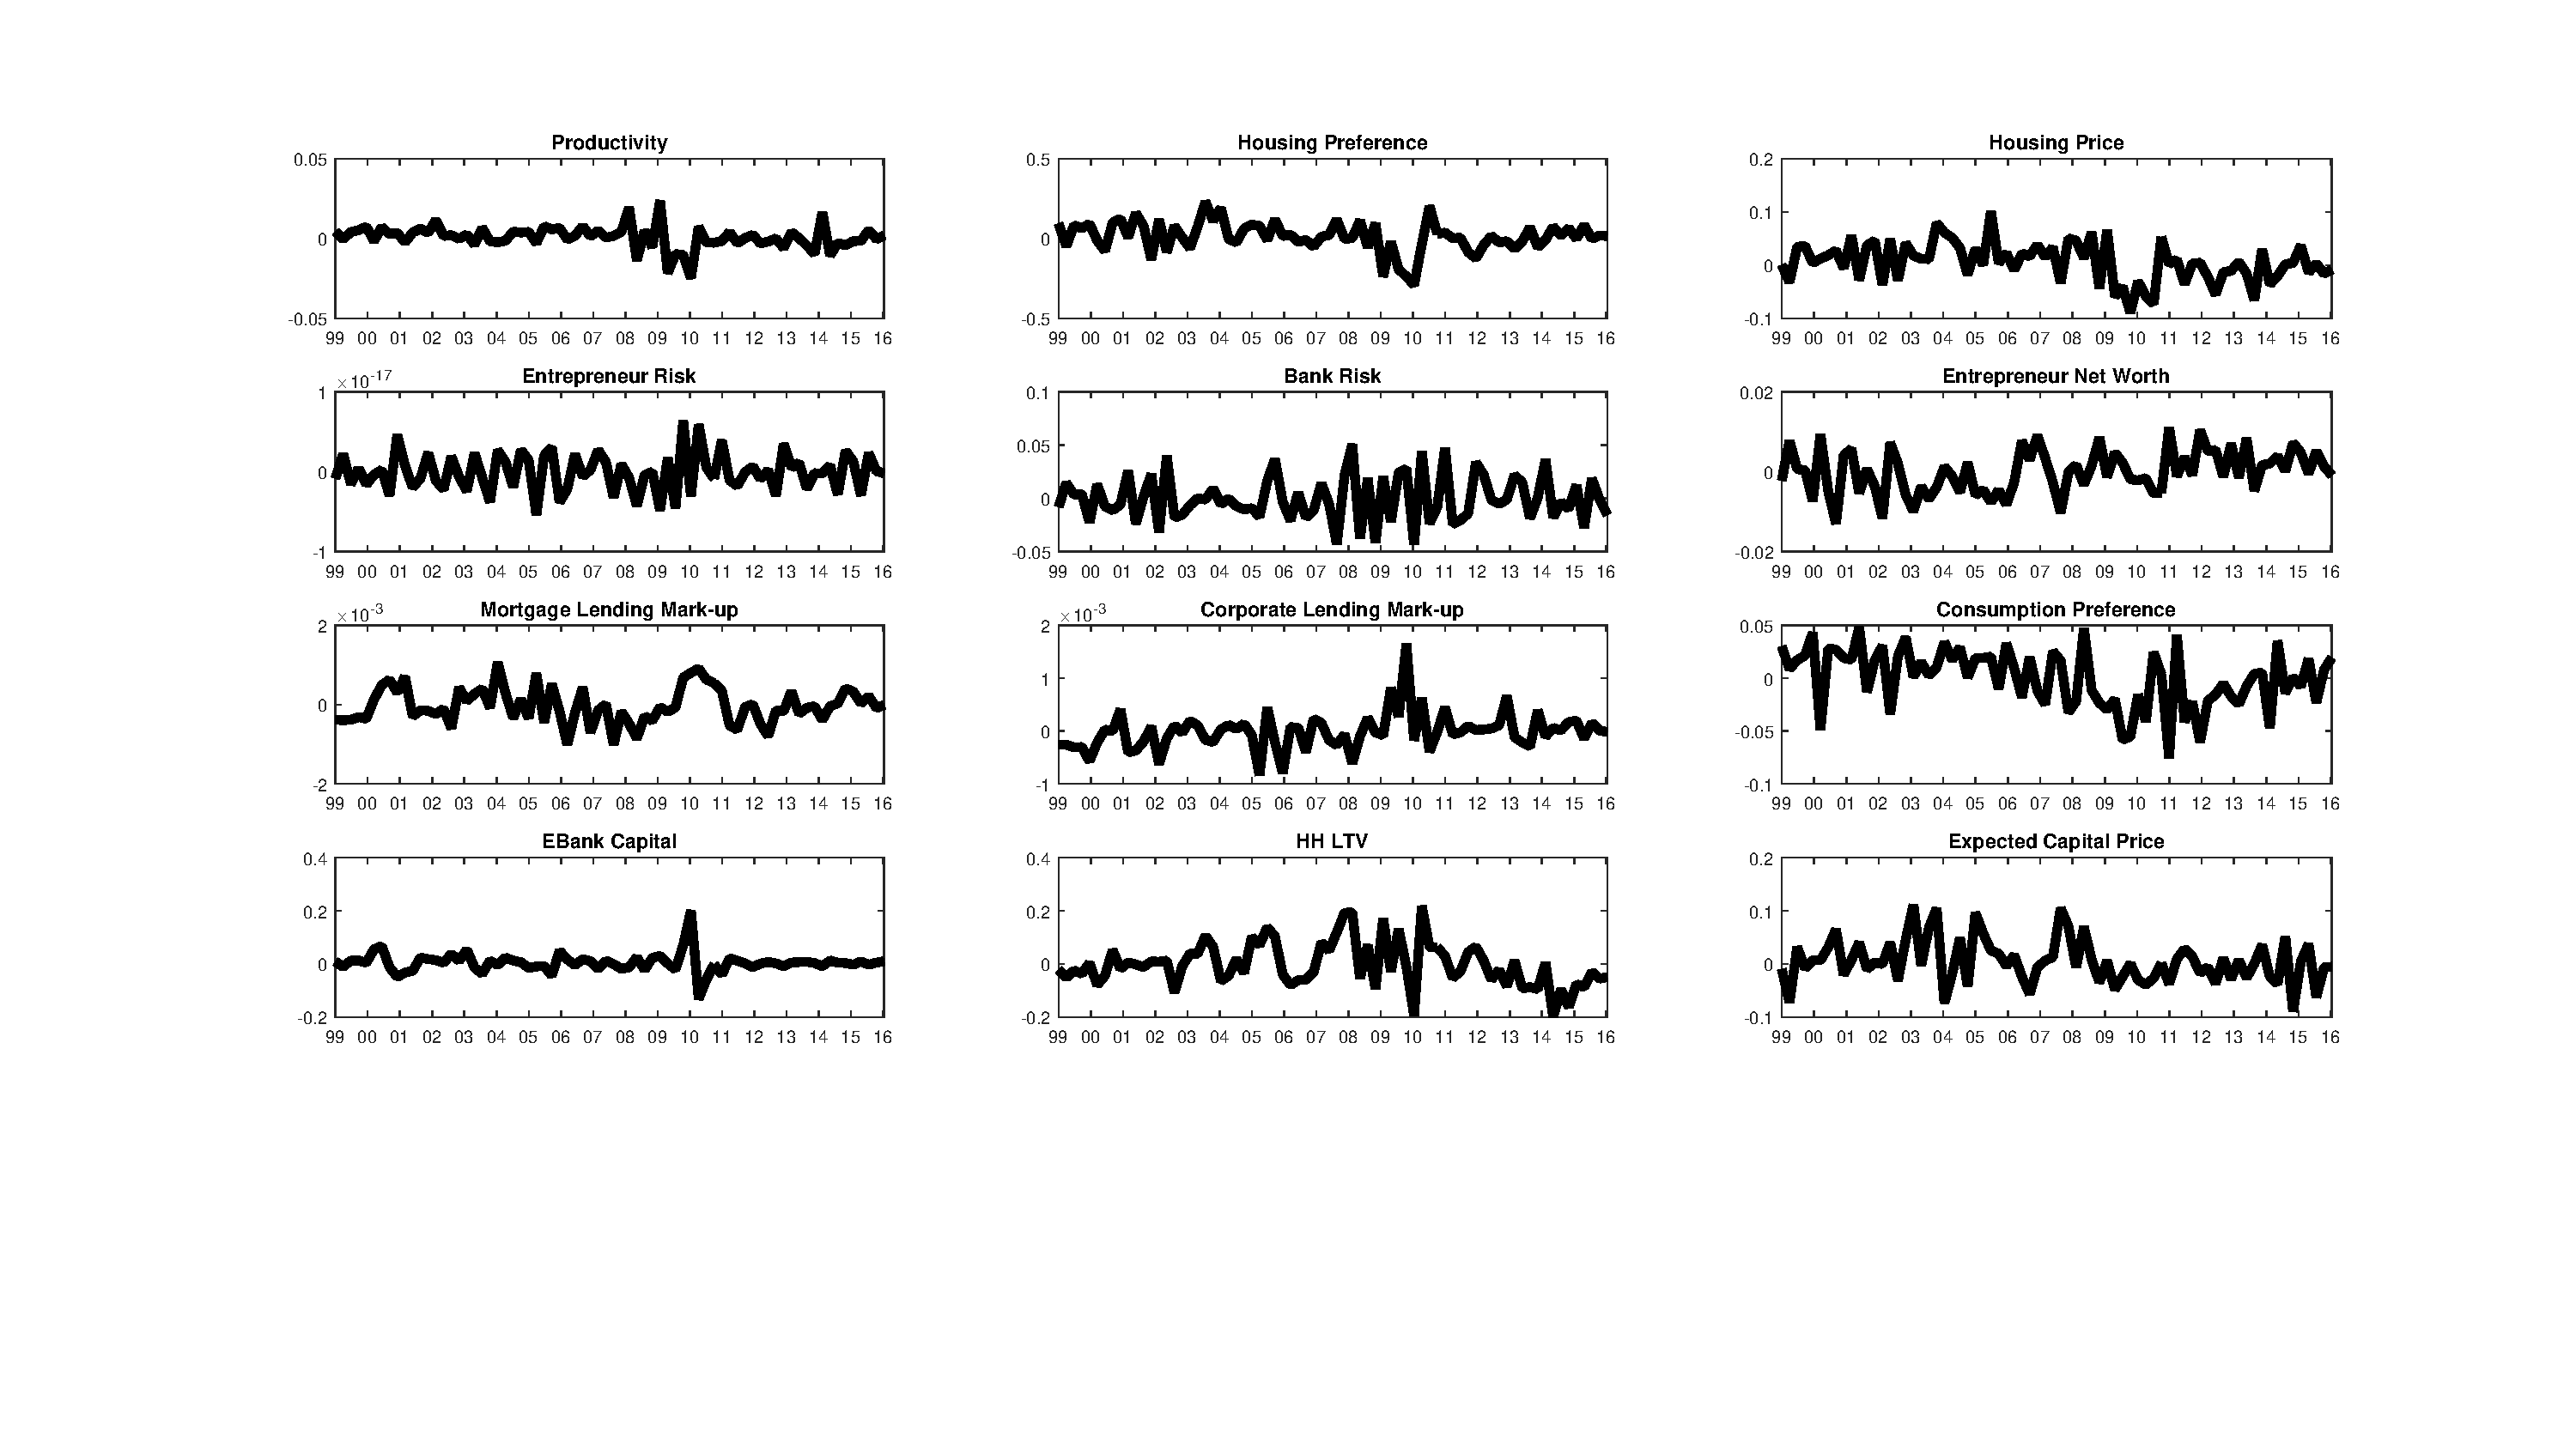
\includegraphics[scale=0.5]{smoothed_shocks.pdf}
%\subfigure[Key shocks driving the financial crisis in the model.]{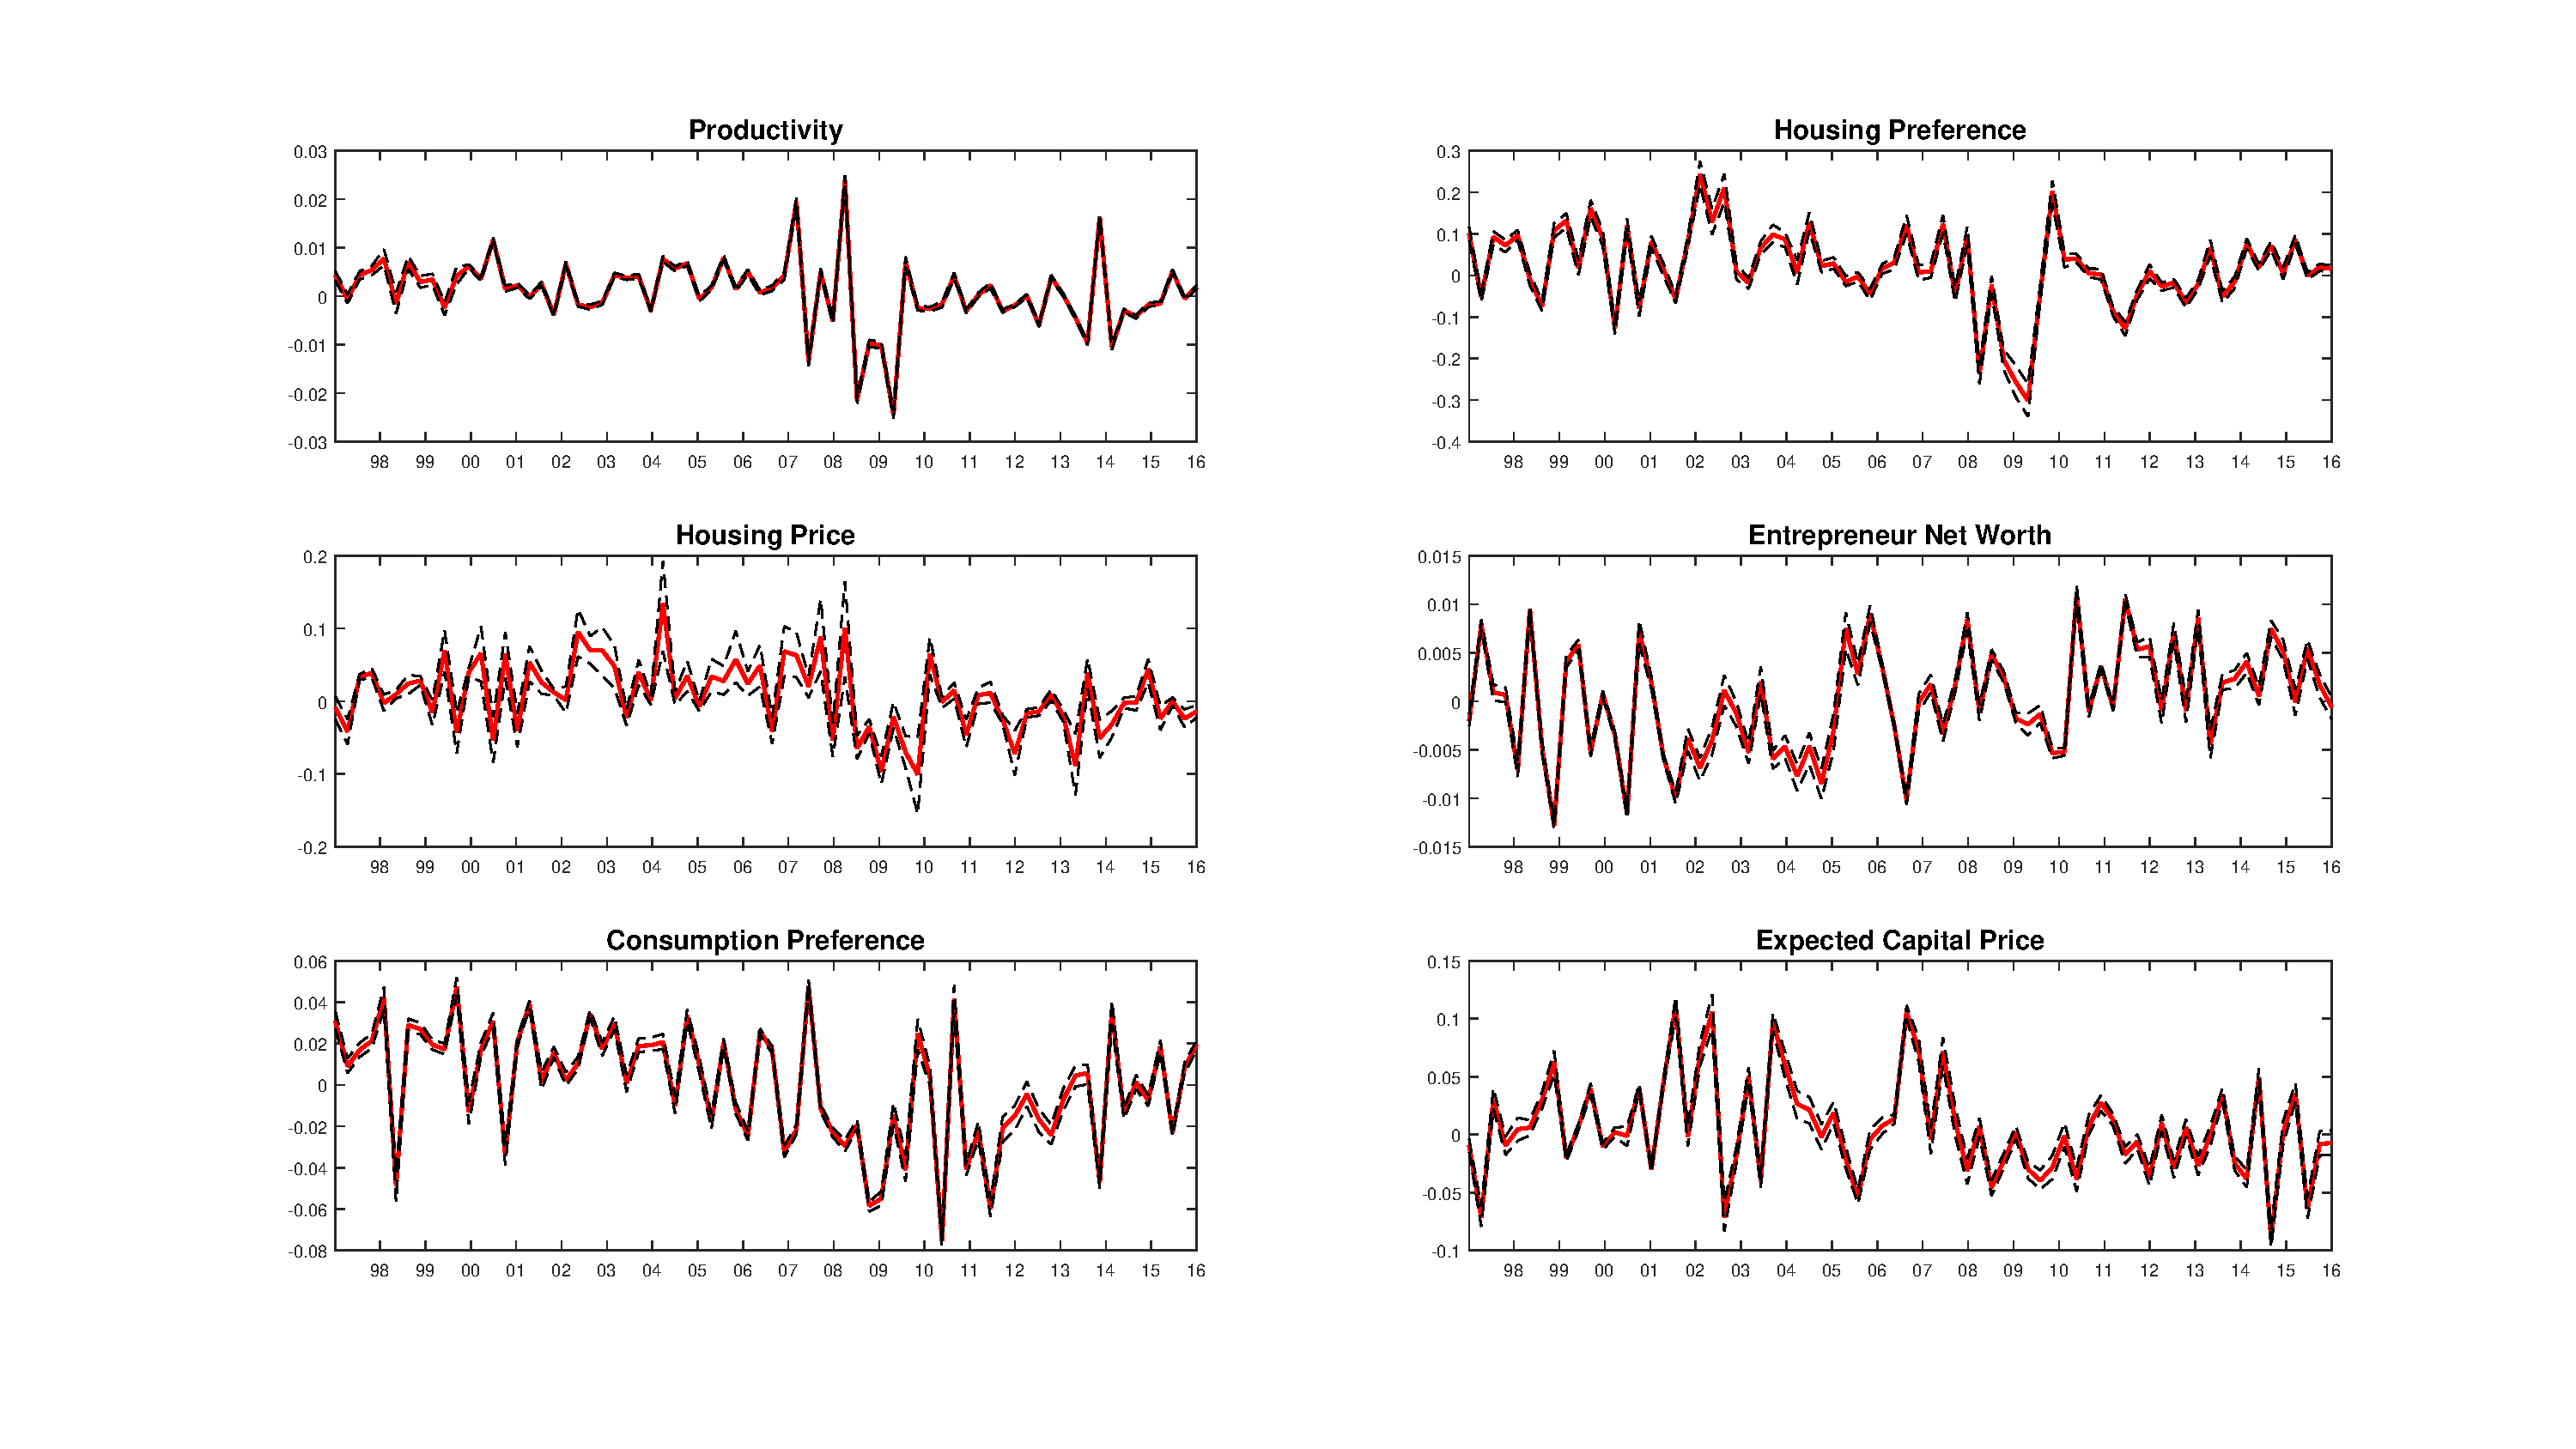
\includegraphics[scale=0.4]{smoothed_shocks_HPD.pdf}}\\
%\subfigure[Default rates during the sample period, where y-axis shows the deviation in percentages from steady-state. ]{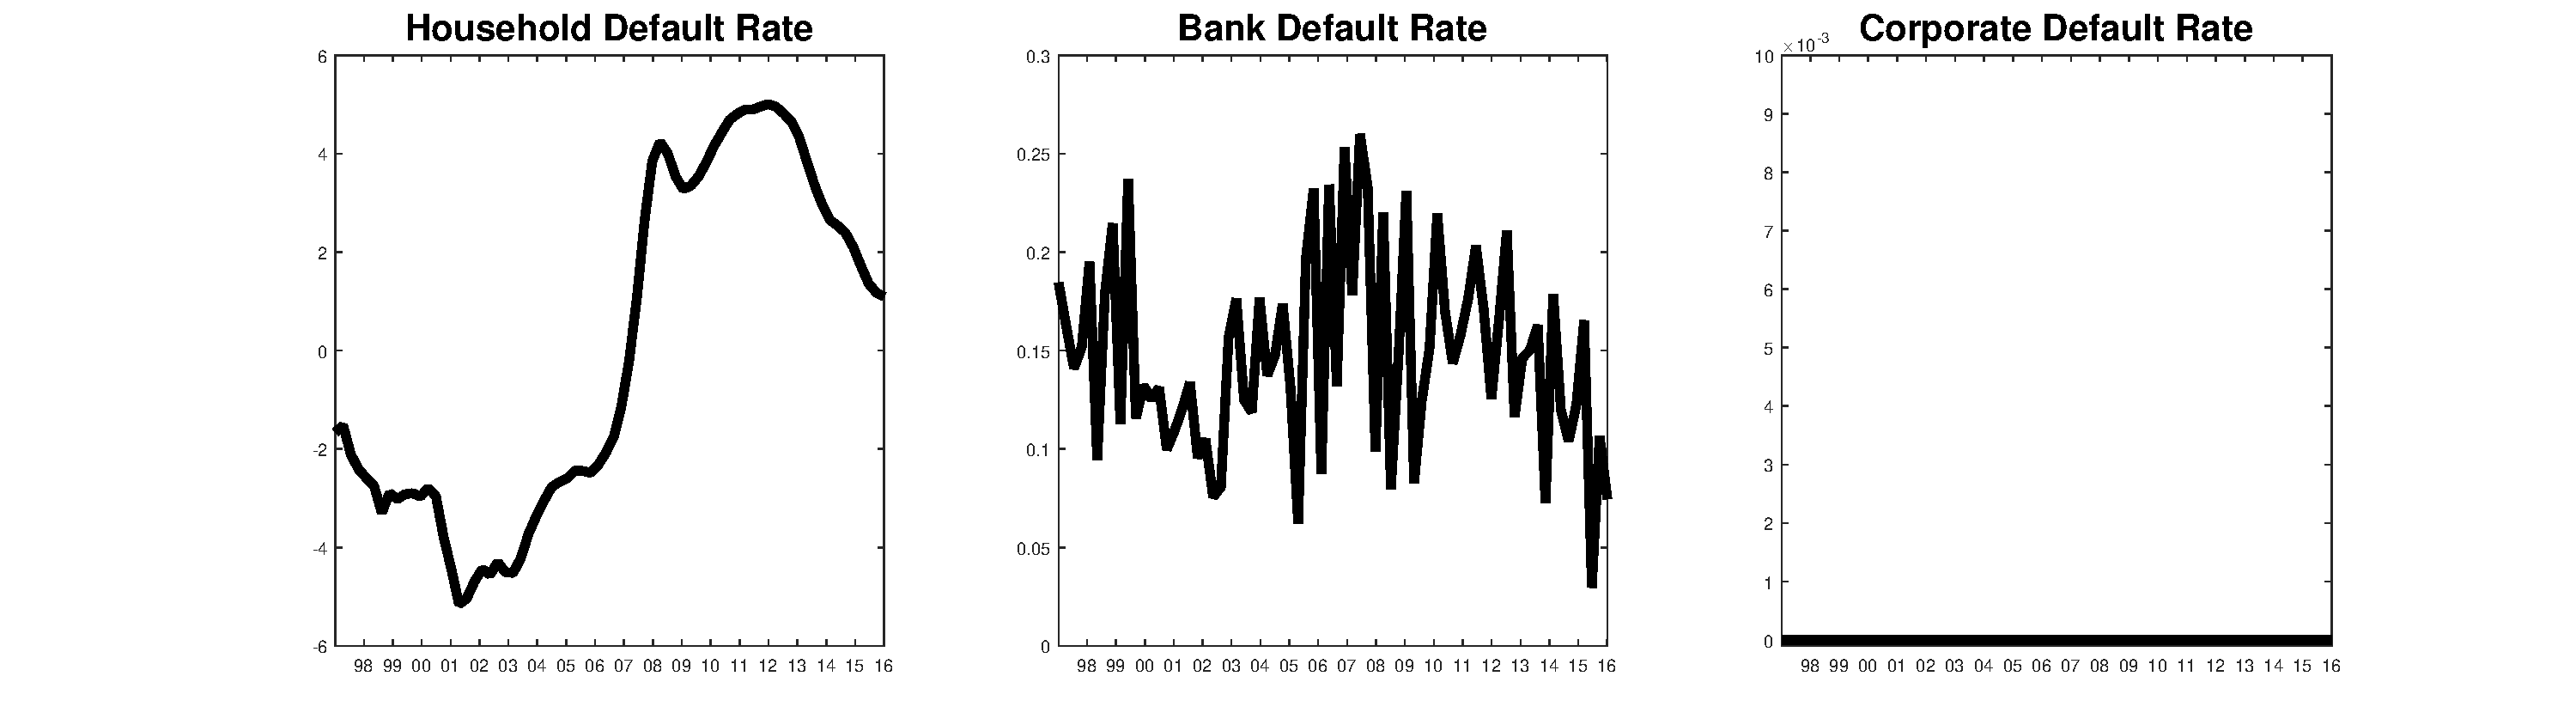
\includegraphics[scale=0.4]{smoothed_default_rates.pdf}}\\
\end{sidewaysfigure}


\begin{sidewaysfigure}
\centering
\caption{Observable variables used in the estimation.}
\label{estimated_shocks}
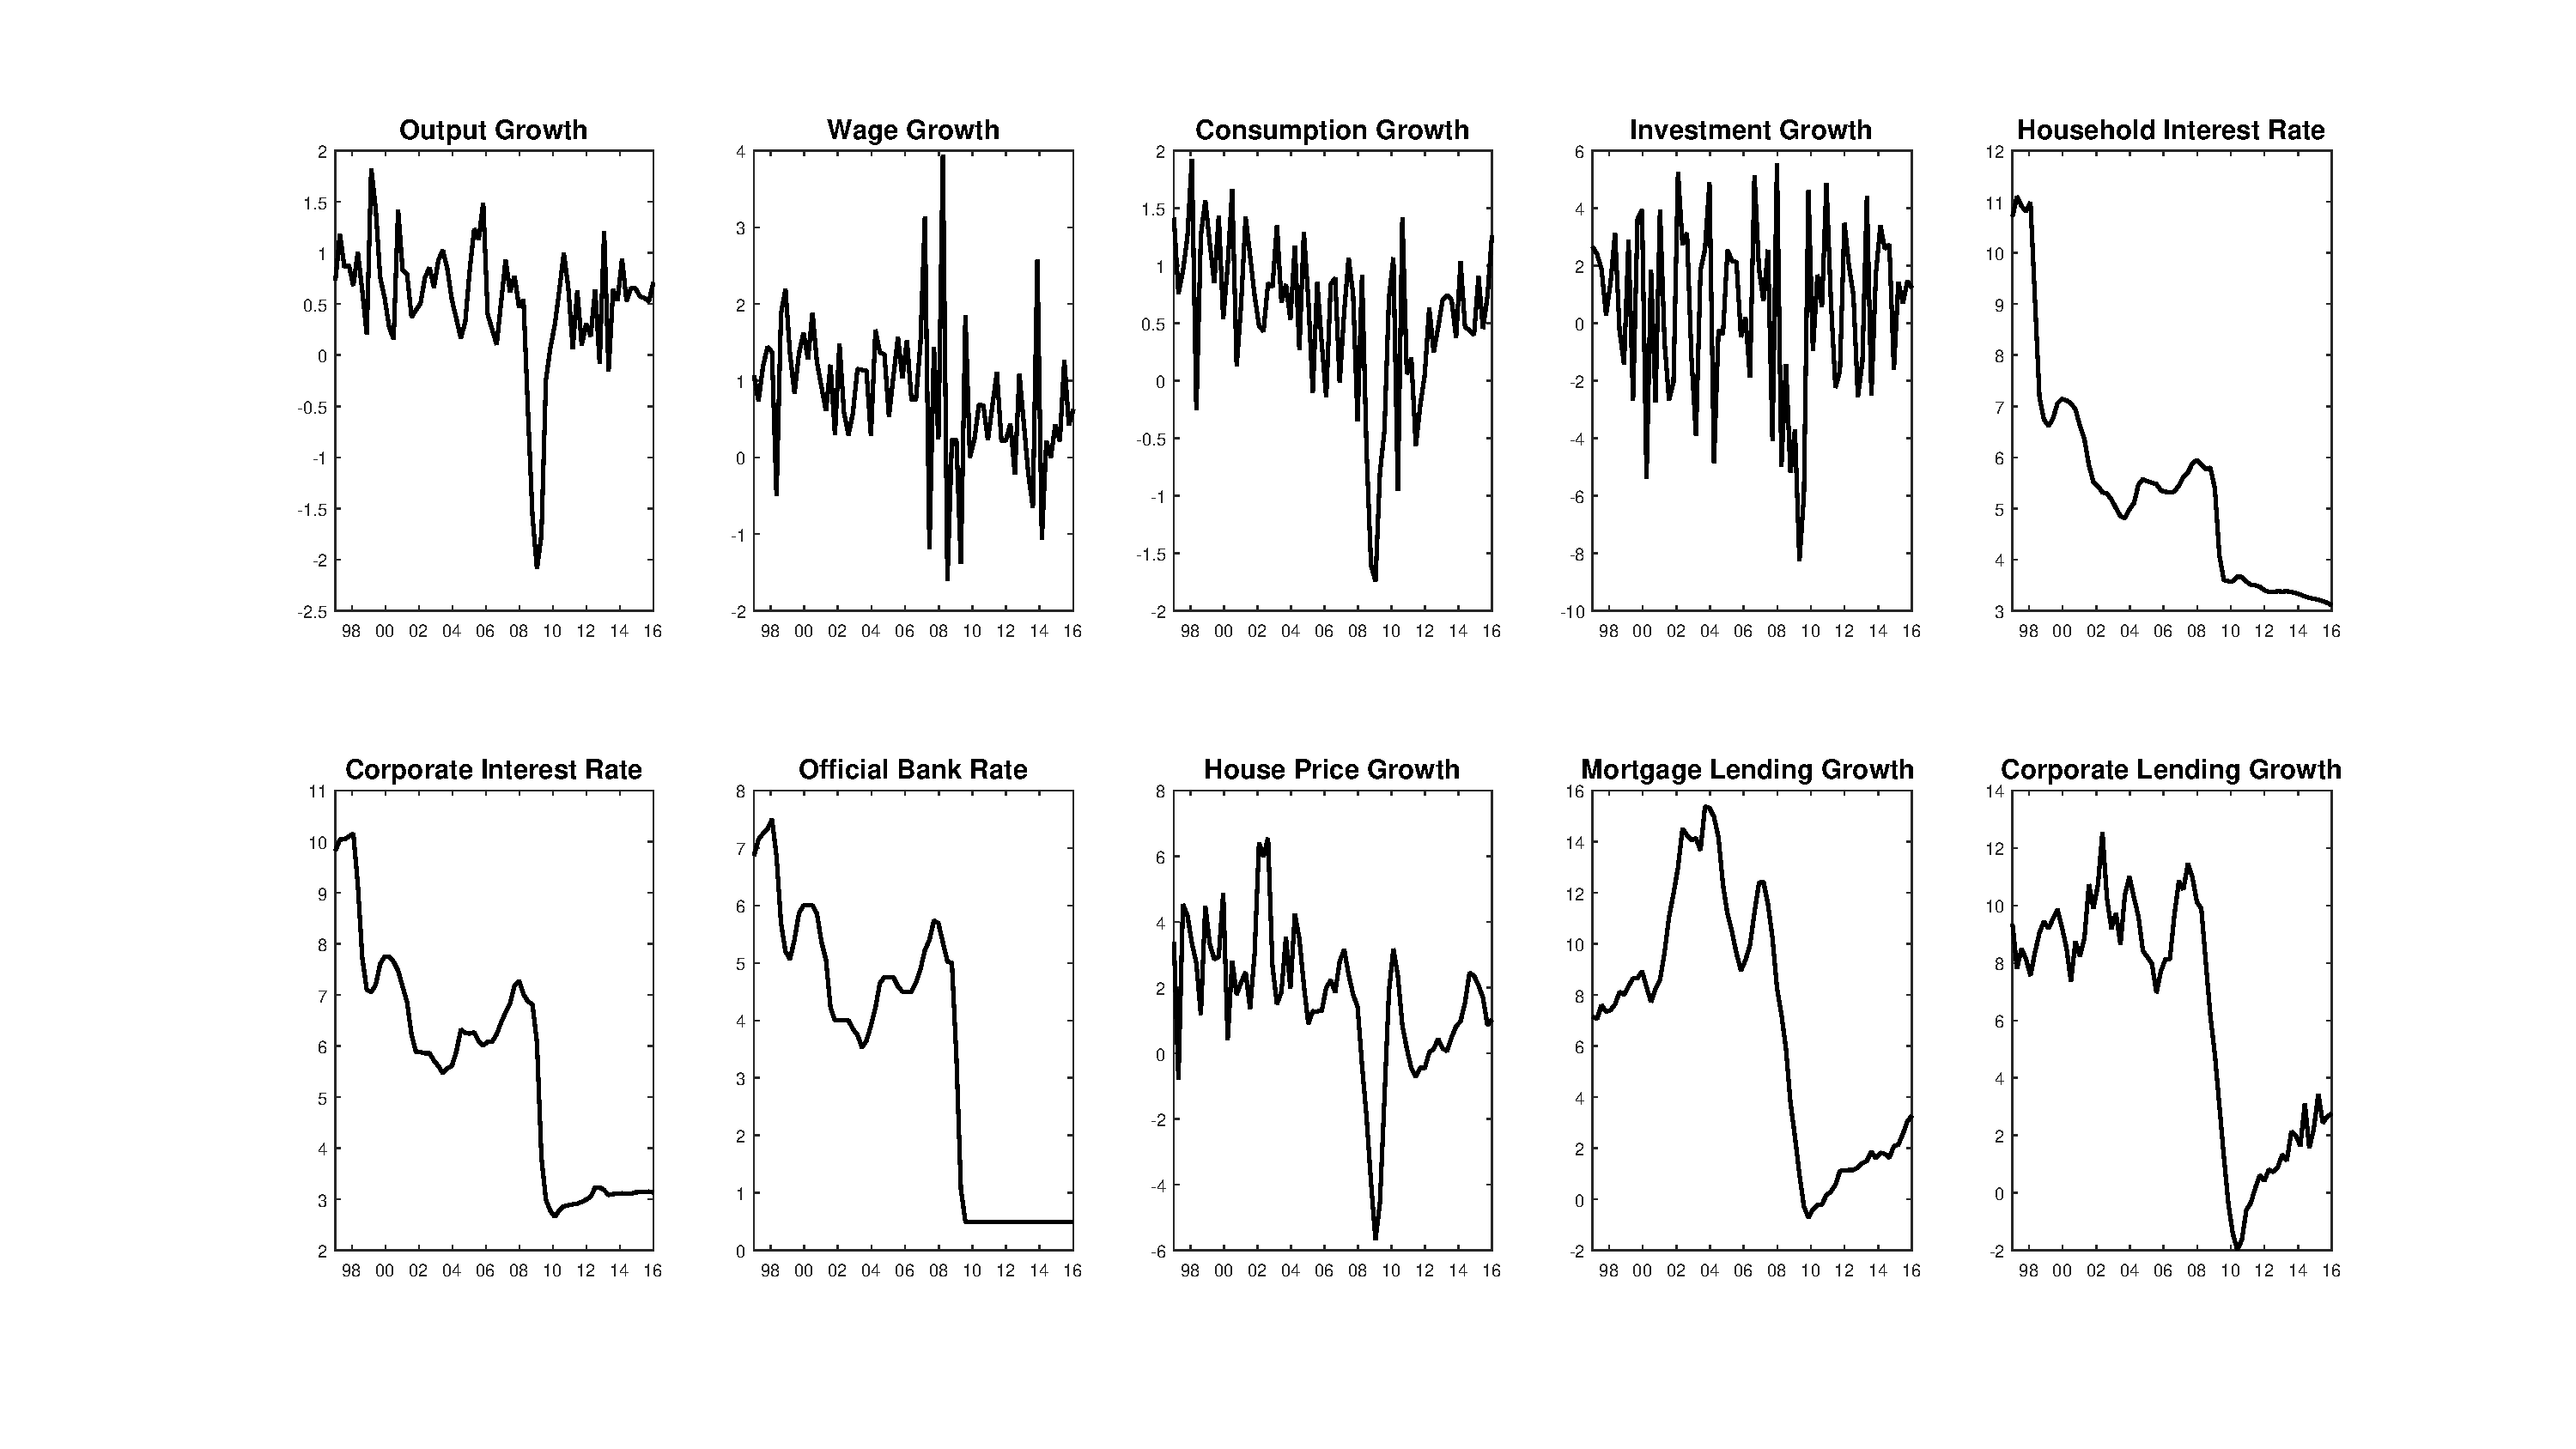
\includegraphics[scale=0.5]{dataset.pdf}
%\subfigure[Key shocks driving the financial crisis in the model.]{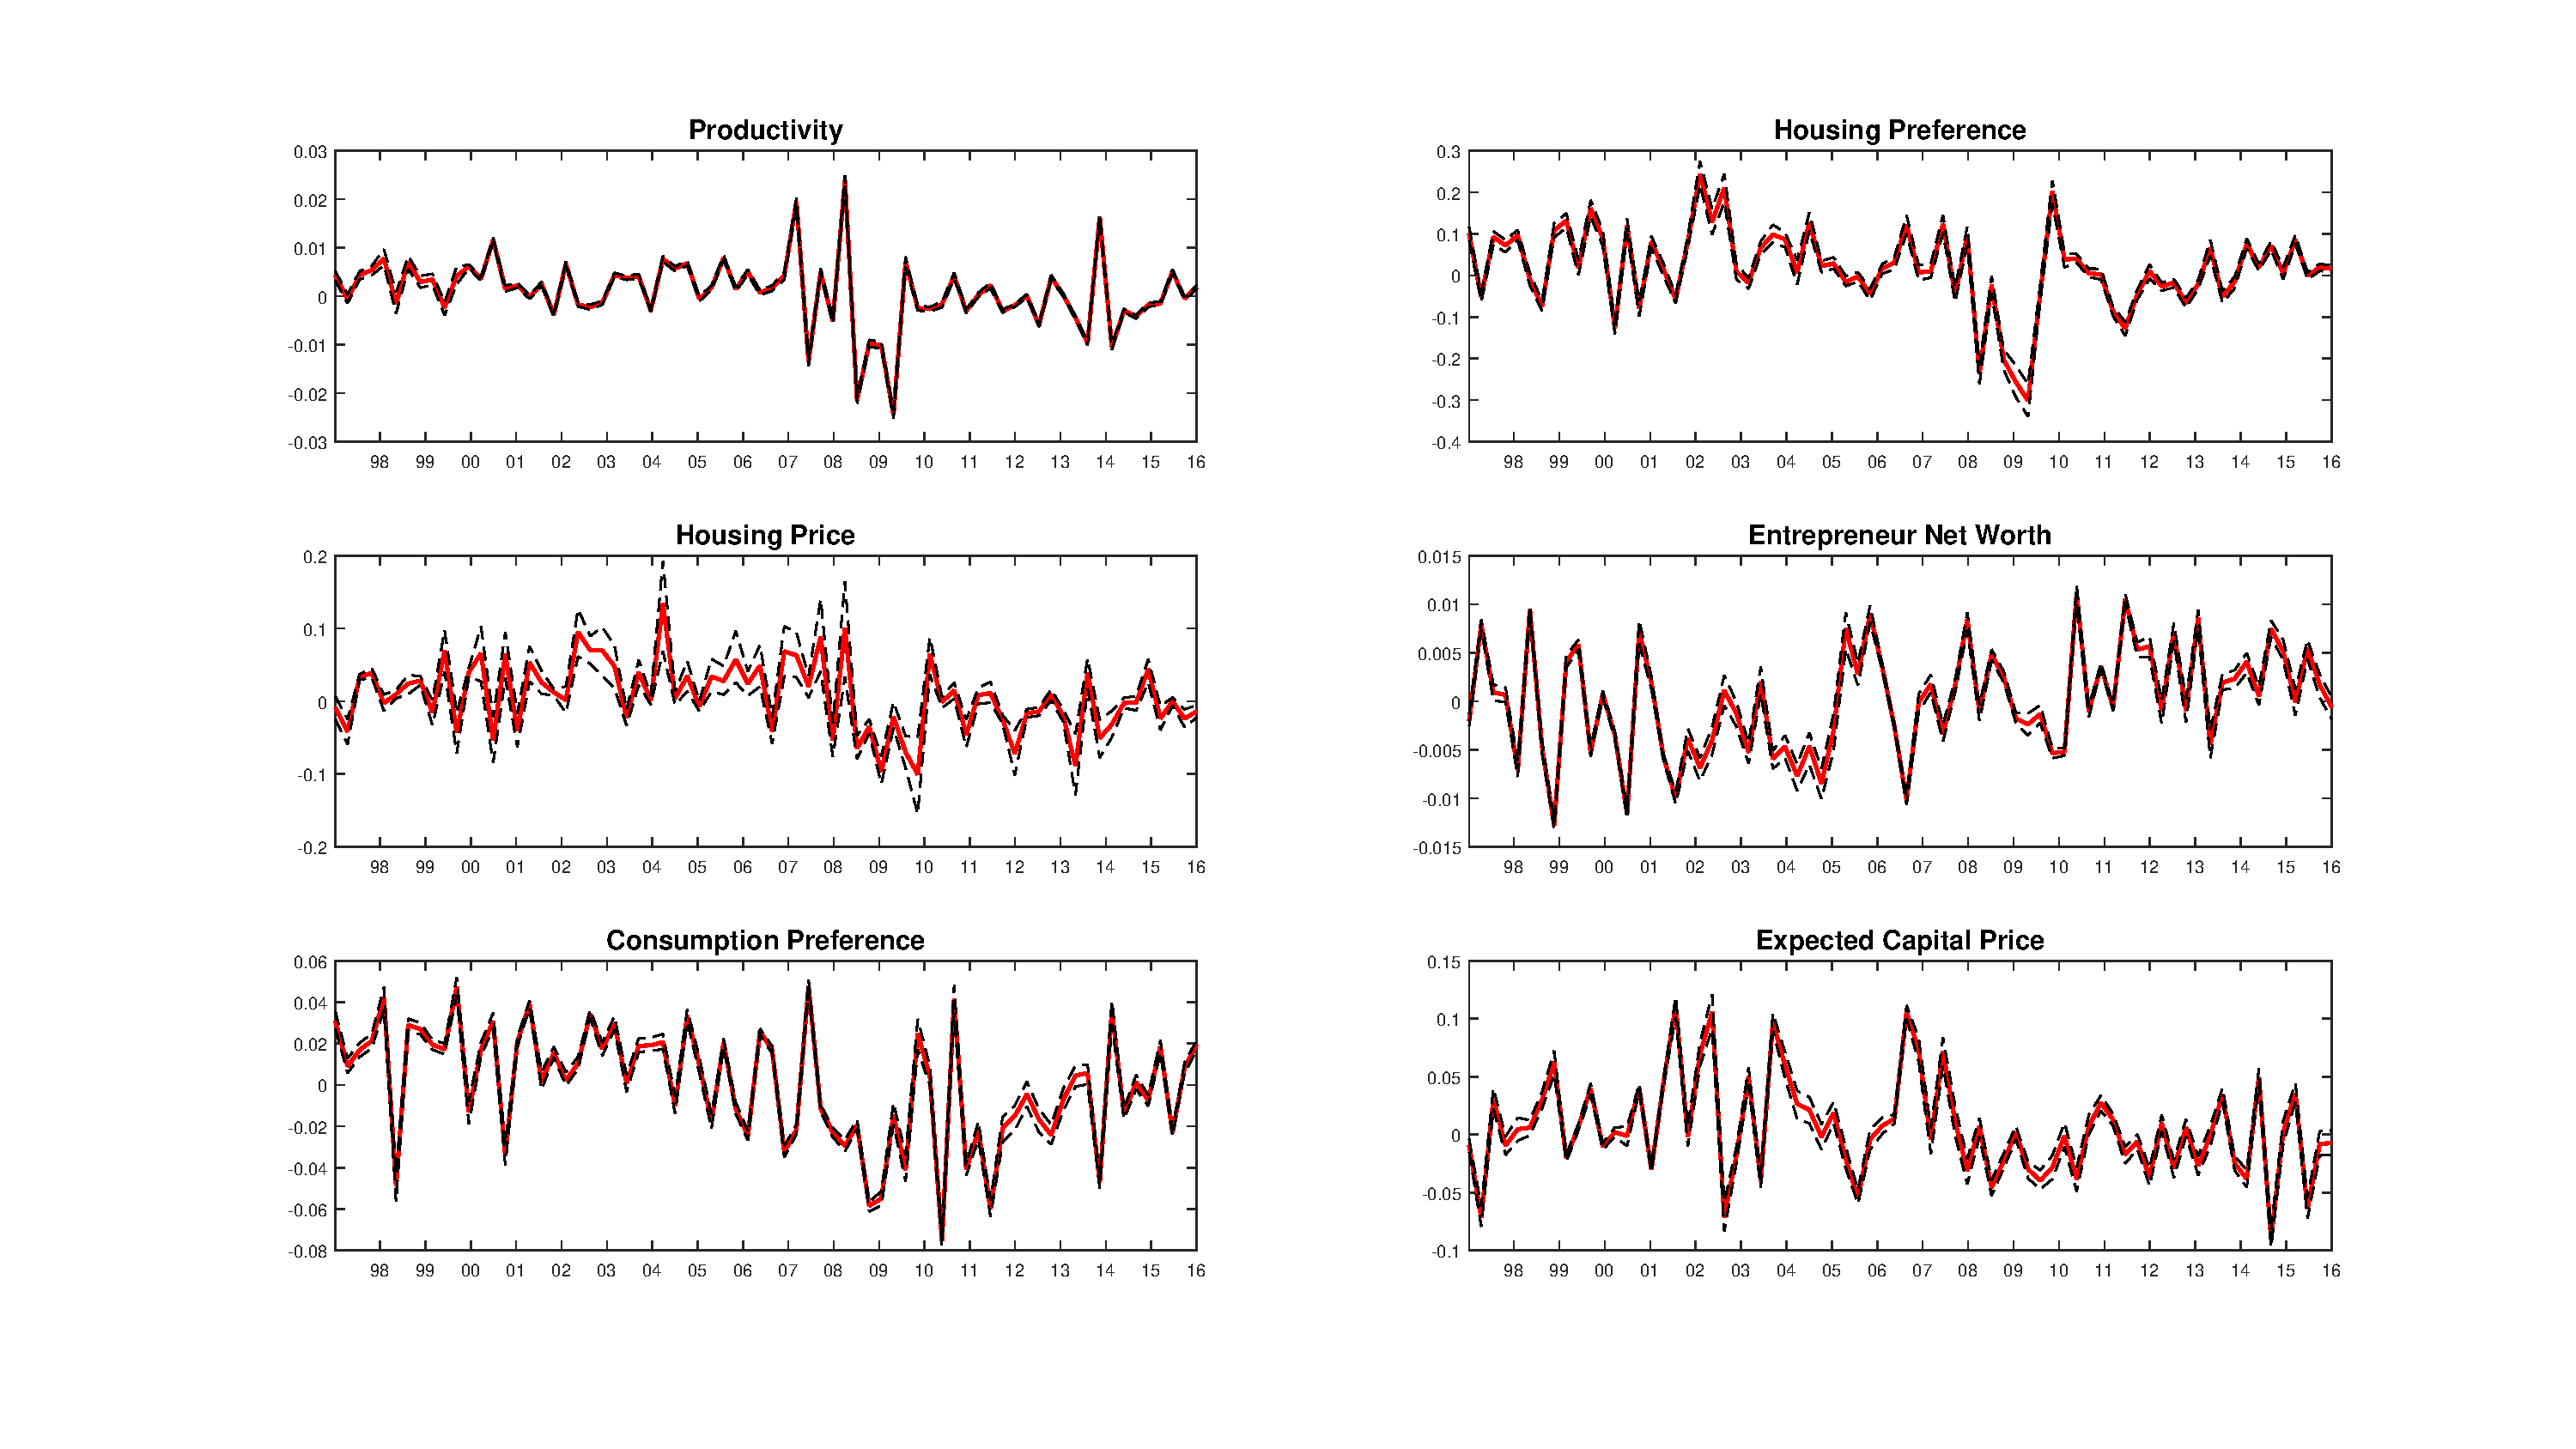
\includegraphics[scale=0.4]{smoothed_shocks_HPD.pdf}}\\
%\subfigure[Default rates during the sample period, where y-axis shows the deviation in percentages from steady-state. ]{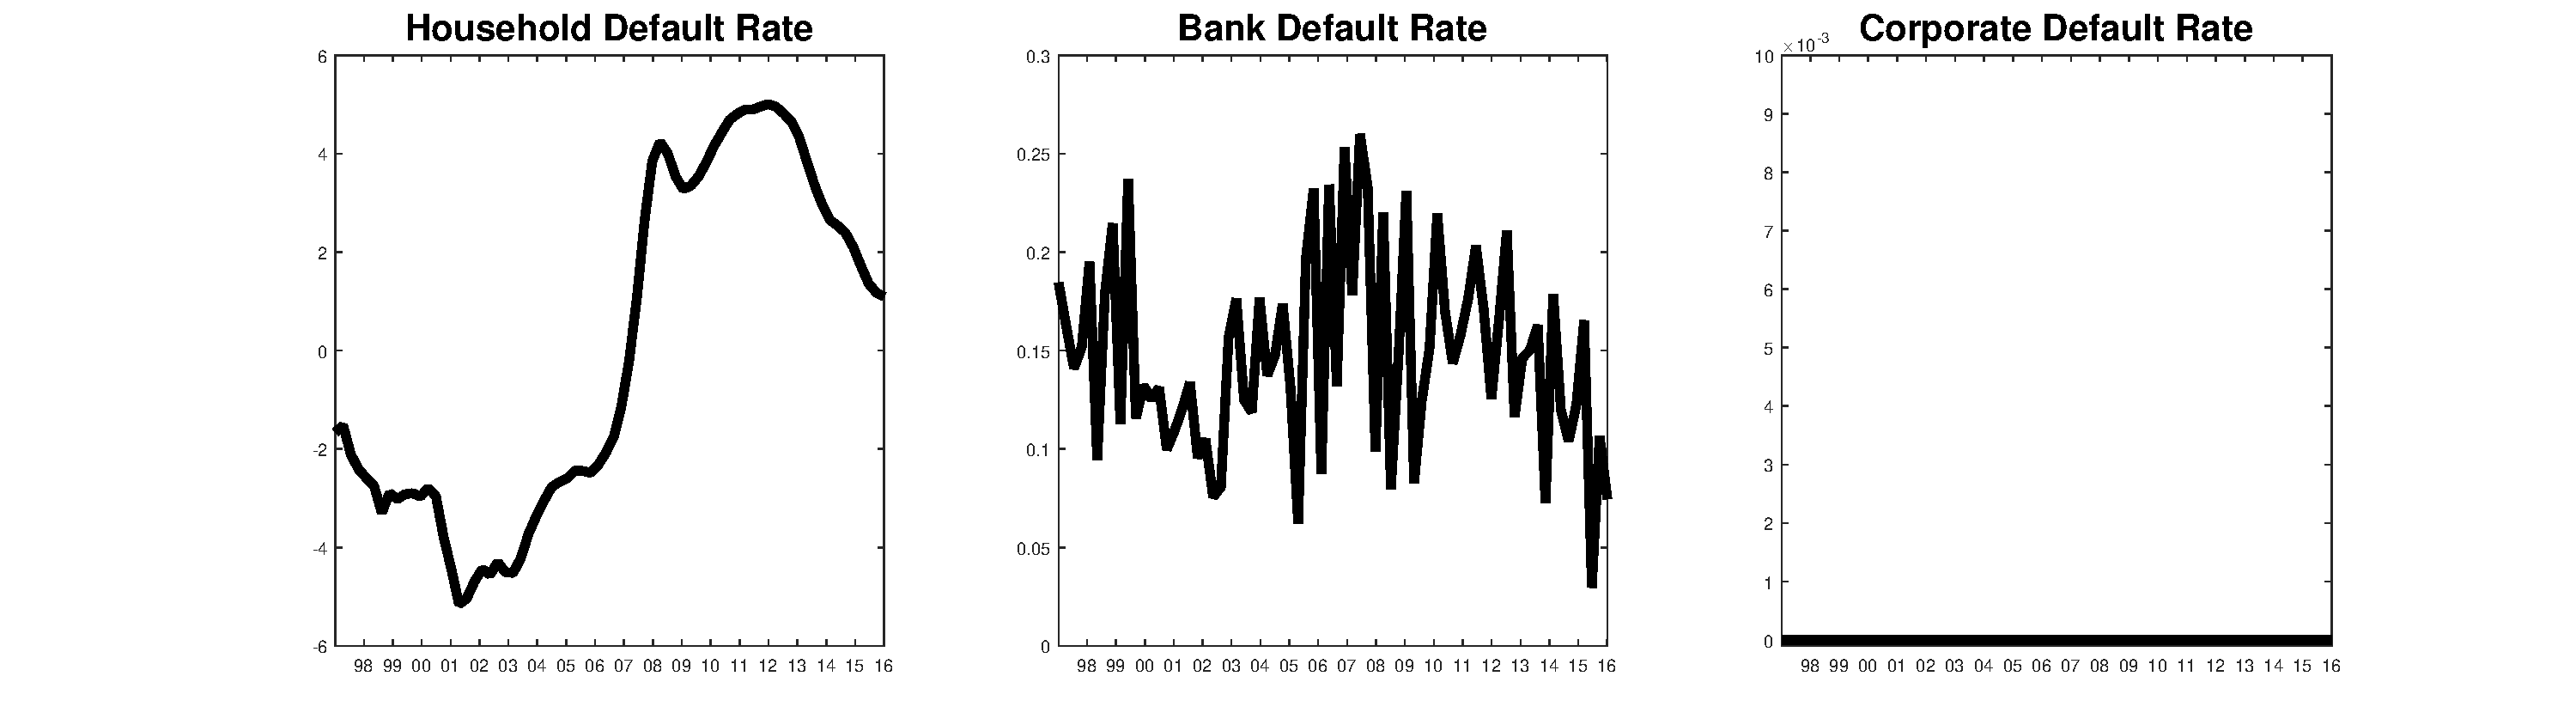
\includegraphics[scale=0.4]{smoothed_default_rates.pdf}}\\
\end{sidewaysfigure}


\FloatBarrier

\section{Cross country evidence on interest rate stickiness}
\label{app_crossCountry}
We do a similar econometric exercise for France, Germany, Italy and Spain. We regress the monthly lending rate with 1 to 5 years of initial rate fixation on ECB policy rate and compare this with the regression of interest floating rate loans on ECB policy rate. We use the data from ECB Statistical Data warehouse.For the fixed rate loans, we use effective interest rate data for loans to corporations with an initial rate fixation  period of over one  to five years. For the floating rate loans, we use effective interest rate data for loans to corporations of (over EUR 1M) and an initial rate fixation period of up to one year.

We find similar results for the Eurozone countries. The response of the lending rate on impact (i.e. during the same month) is very small. In case of variable interest rate loans,the bulk of adjustment takes place in the following period, whereas the adjustment in fixed rate loans is reflected over a longer period.
 
\begin {table}[H]
\caption {Regression of 1 to 5 year lending rate on ECB policy rate} \label{tab:title} 
\begin{center}
	\begin{tabular}{||c c c c c||} 
		\hline
		Regressor &  France & Germany& Italy & Spain \\ [0.5ex] 
		\hline\hline
		$\i_{t}$ & $0.054^{***}$& $0.015^{***}$ & $0.014^{**}$& $0.0027$ \\ 
		\hline
		$\Delta$ $\i_{t-1}$& $0.257^{***}$& $0.246^{***}$& $0.258^{***}$& $0.151^{**}$ \\ 
		\hline
		$\Delta$ $\i_{t-2}$&$0.316^{***}$ &-$0.009$& $0.124^{***}$& $0.215^{**}$ \\
		
		\hline
		$\Delta$ $\i_{t-3}$	&  $0.294^{***}$ &  $0.134^{***}$& $0.17^{***}$& $0.203^{**}$ \\
		\hline
		$\Delta$  $\i_{t-4}$&-$0.249^{*}$&-$0.04$ & -$0.119^{**}$& -$0.049$ \\  
		\hline
		$\Delta$  $\i_{t-5}$&$0.366^{***}$&$0.033$ & -$0.09$& -$0.047^{**}$ \\  
		\hline
		constant&$0.105^{***}$ &$0.035^{***}$& $0.046^{**}$ & $0.014$\\ 
		
		\hline
			
		\end{tabular}
\end{center}
\end {table}




\begin {table}[H]
\caption {Regression of floating year lending rate on ECB policy rate} \label{tab:title} 
\begin{center}
	\begin{tabular}{||c c c c c||} 
		\hline
		Regressor &  France & Germany& Italy & Spain \\ [0.5ex] 
		\hline\hline
		$\i_{t}$ & $0.0729^{***}$& $0.137^{***}$ & $0.034^{**}$& $0.045^{**}$ \\ 
		\hline
		$\Delta$ $\i_{t-1}$& $0.766^{***}$& $0.481^{***}$& $0.597^{***}$& $0.670^{**}$ \\ 
		\hline
		$\Delta$ $\i_{t-2}$&- $0.009$ &$0.389^{***}$& $0.251^{***}$& $0.203$ \\
		
		\hline
		$\Delta$ $\i_{t-3}$	&  $0.577^{***}$ &  $0.1915$& $0.284^{***}$& $0.466^{**}$ \\
		\hline
		$\Delta$  $\i_{t-4}$&-$0.07$&-$0.157$ & $0.049$& -$0.333^{*}$ \\  
		\hline
		$\Delta$  $\i_{t-5}$&$0.09$&$0.017$ & $0.0165$& -$0.0165$ \\  
		\hline
		constant&$0.139^{***}$ &$0.158^{***}$& $0.08^{**}$ & $0.153^{**}$\\ 
		
		\hline
		
	\end{tabular}
\end{center}
\end {table}


The above table shows that the interest rate pass through in France.In response to 1 percentage point change in policy rate, there is less than 0.05 percentage point change in the fixed term lending rate on impact.  Around 0.25 percentage point change in interest rate is passed through during the following month and around 0.3 percentage point change is passed through during the third and fourth months after the policy rate change.

For the floating interest rate loans, the response on impact is also low. However,around 76 percent of the pass through takes place in the following month and there is a complete pass through by the end of four months.



The above table shows that the interest rate pass through in Germany.In response to 1 percentage point change in policy rate, there is less than 0.015 percentage point change in the fixed term lending rate on impact.  Around 0.25 percentage point change in interest rate is passed through during the following month and around 0.13 percentage point change is passed through during the fourth month after the policy rate change.

For the floating interest rate loans, the response on impact is also low. However,around 48 percent of the pass through takes place in the following month and there is a complete pass through by the end of four months.


The above table shows that the interest rate pass through in Italy.In response to 1 percentage point change in policy rate, there is less than 0.015 percentage point change in the fixed term lending rate on impact.  Around around 0.26 percentage point change in interest rate is passed through during the following month and around 0.12 and 0.17 percentage point change is passed through during the third month and fourth months after the policy rate change.

For the floating interest rate loans, the response on impact is also low. However,around 60 percent of the pass through takes place in the following month and there is a complete pass through by the end of four months.



The above table shows that the interest rate pass through in Spain.In response to 1 percentage point change in policy rate, there is less than 0.01 percentage point change in the fixed term lending rate on impact.  Only around 0.15 percentage point change in interest rate is passed through during the following month and around 0.2  change is passed through during the third month and fourth months after the policy rate change

For the floating interest rate loans, the response on impact is also low. However,around 67 percent of the pass through takes place in the following month and there is a complete pass through by the end of four months.

To sum up,there is a clear pattern which emerges for all the four Eurozone economies.The response of fixed term lending rates on impact is very low.Around 25 per cent of the pass through takes place in the following period and around 20 to 30 per cent of the pass through takes place in the third and fourth months. Overall, the pass through of interest rate for fixed term loans is incomplete as observed in the UK data.

For the floating interest rate loans, the on impact is also low. However,around 50 to 70 percent of the pass through takes place in the following month and there is a complete pass through by the end of four months.

On the whole, we find that interest rate pass through is fastest in France as compared to Germany where it is the slowest among the four Eurozone economies.

\section{Posterior distributions of all estimated parameters}
\label{app_posteriorDist}

\begin{figure}[h]
\centering
\caption{Posterior Parameter Distributions}
\label{app_post1}
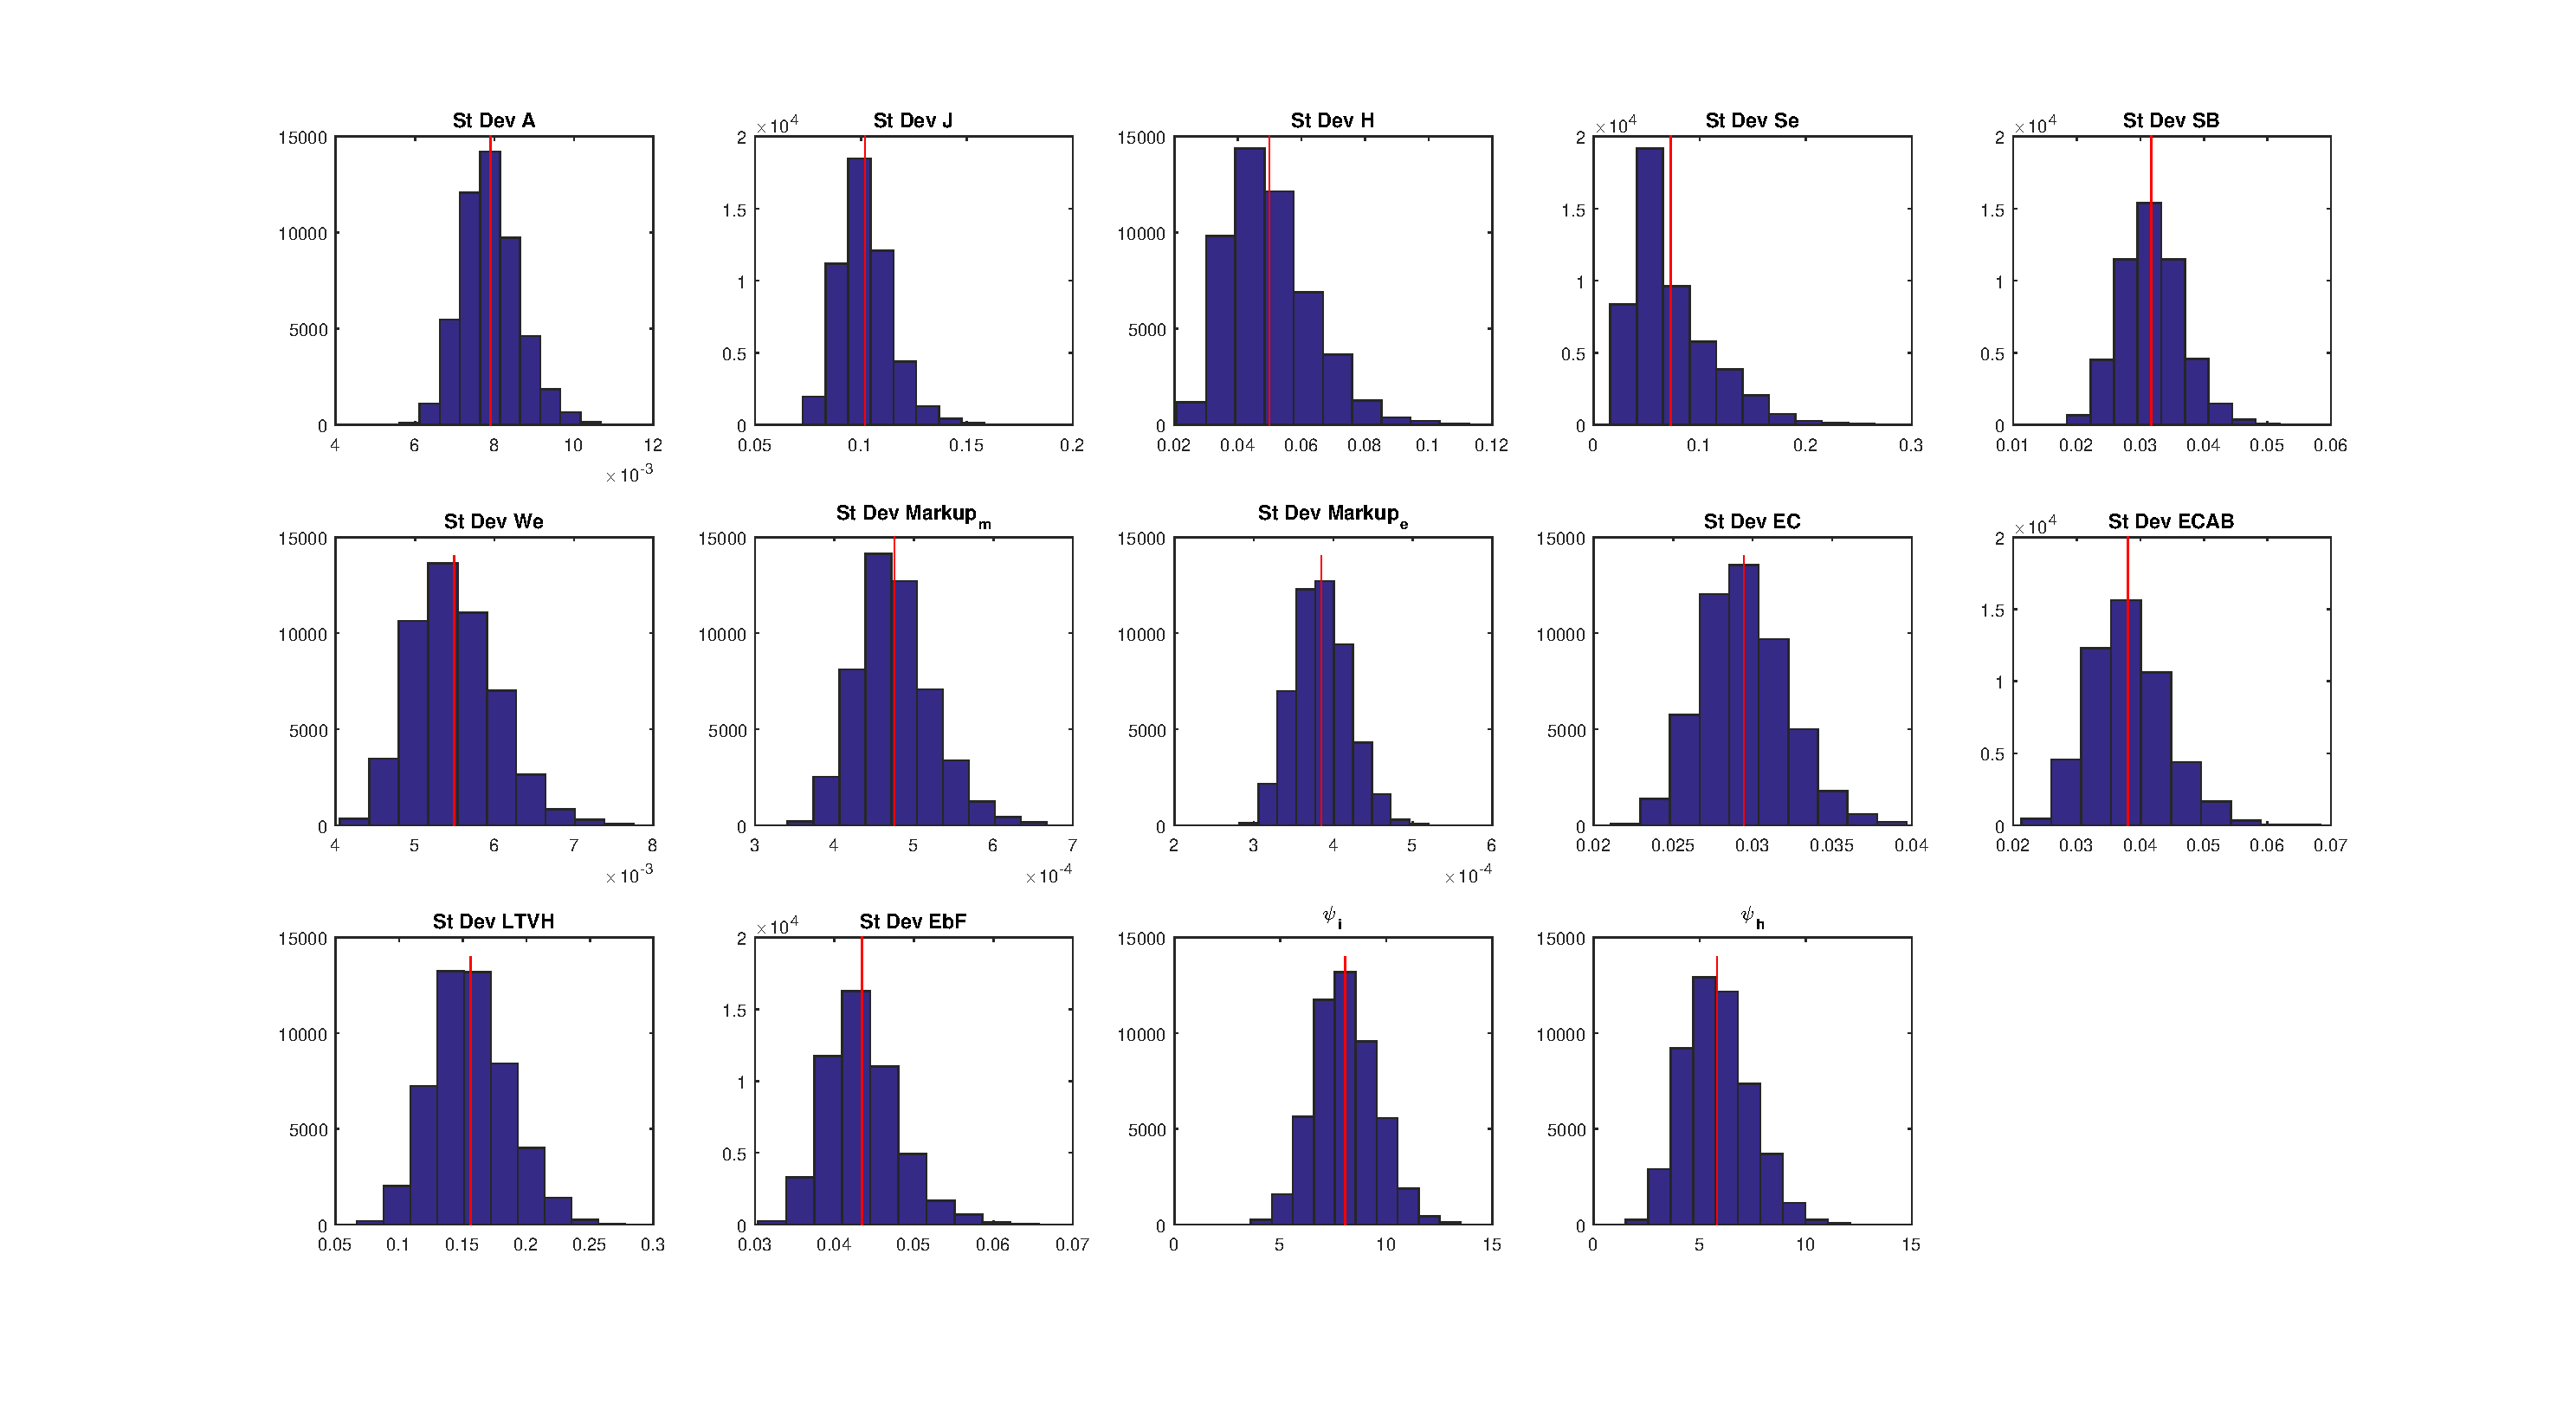
\includegraphics[scale=0.45]{posteriordistributions1.pdf}
\end{figure}

\begin{figure}[h]
\centering
\caption{Posterior Parameter Distributions}
\label{app_post2}
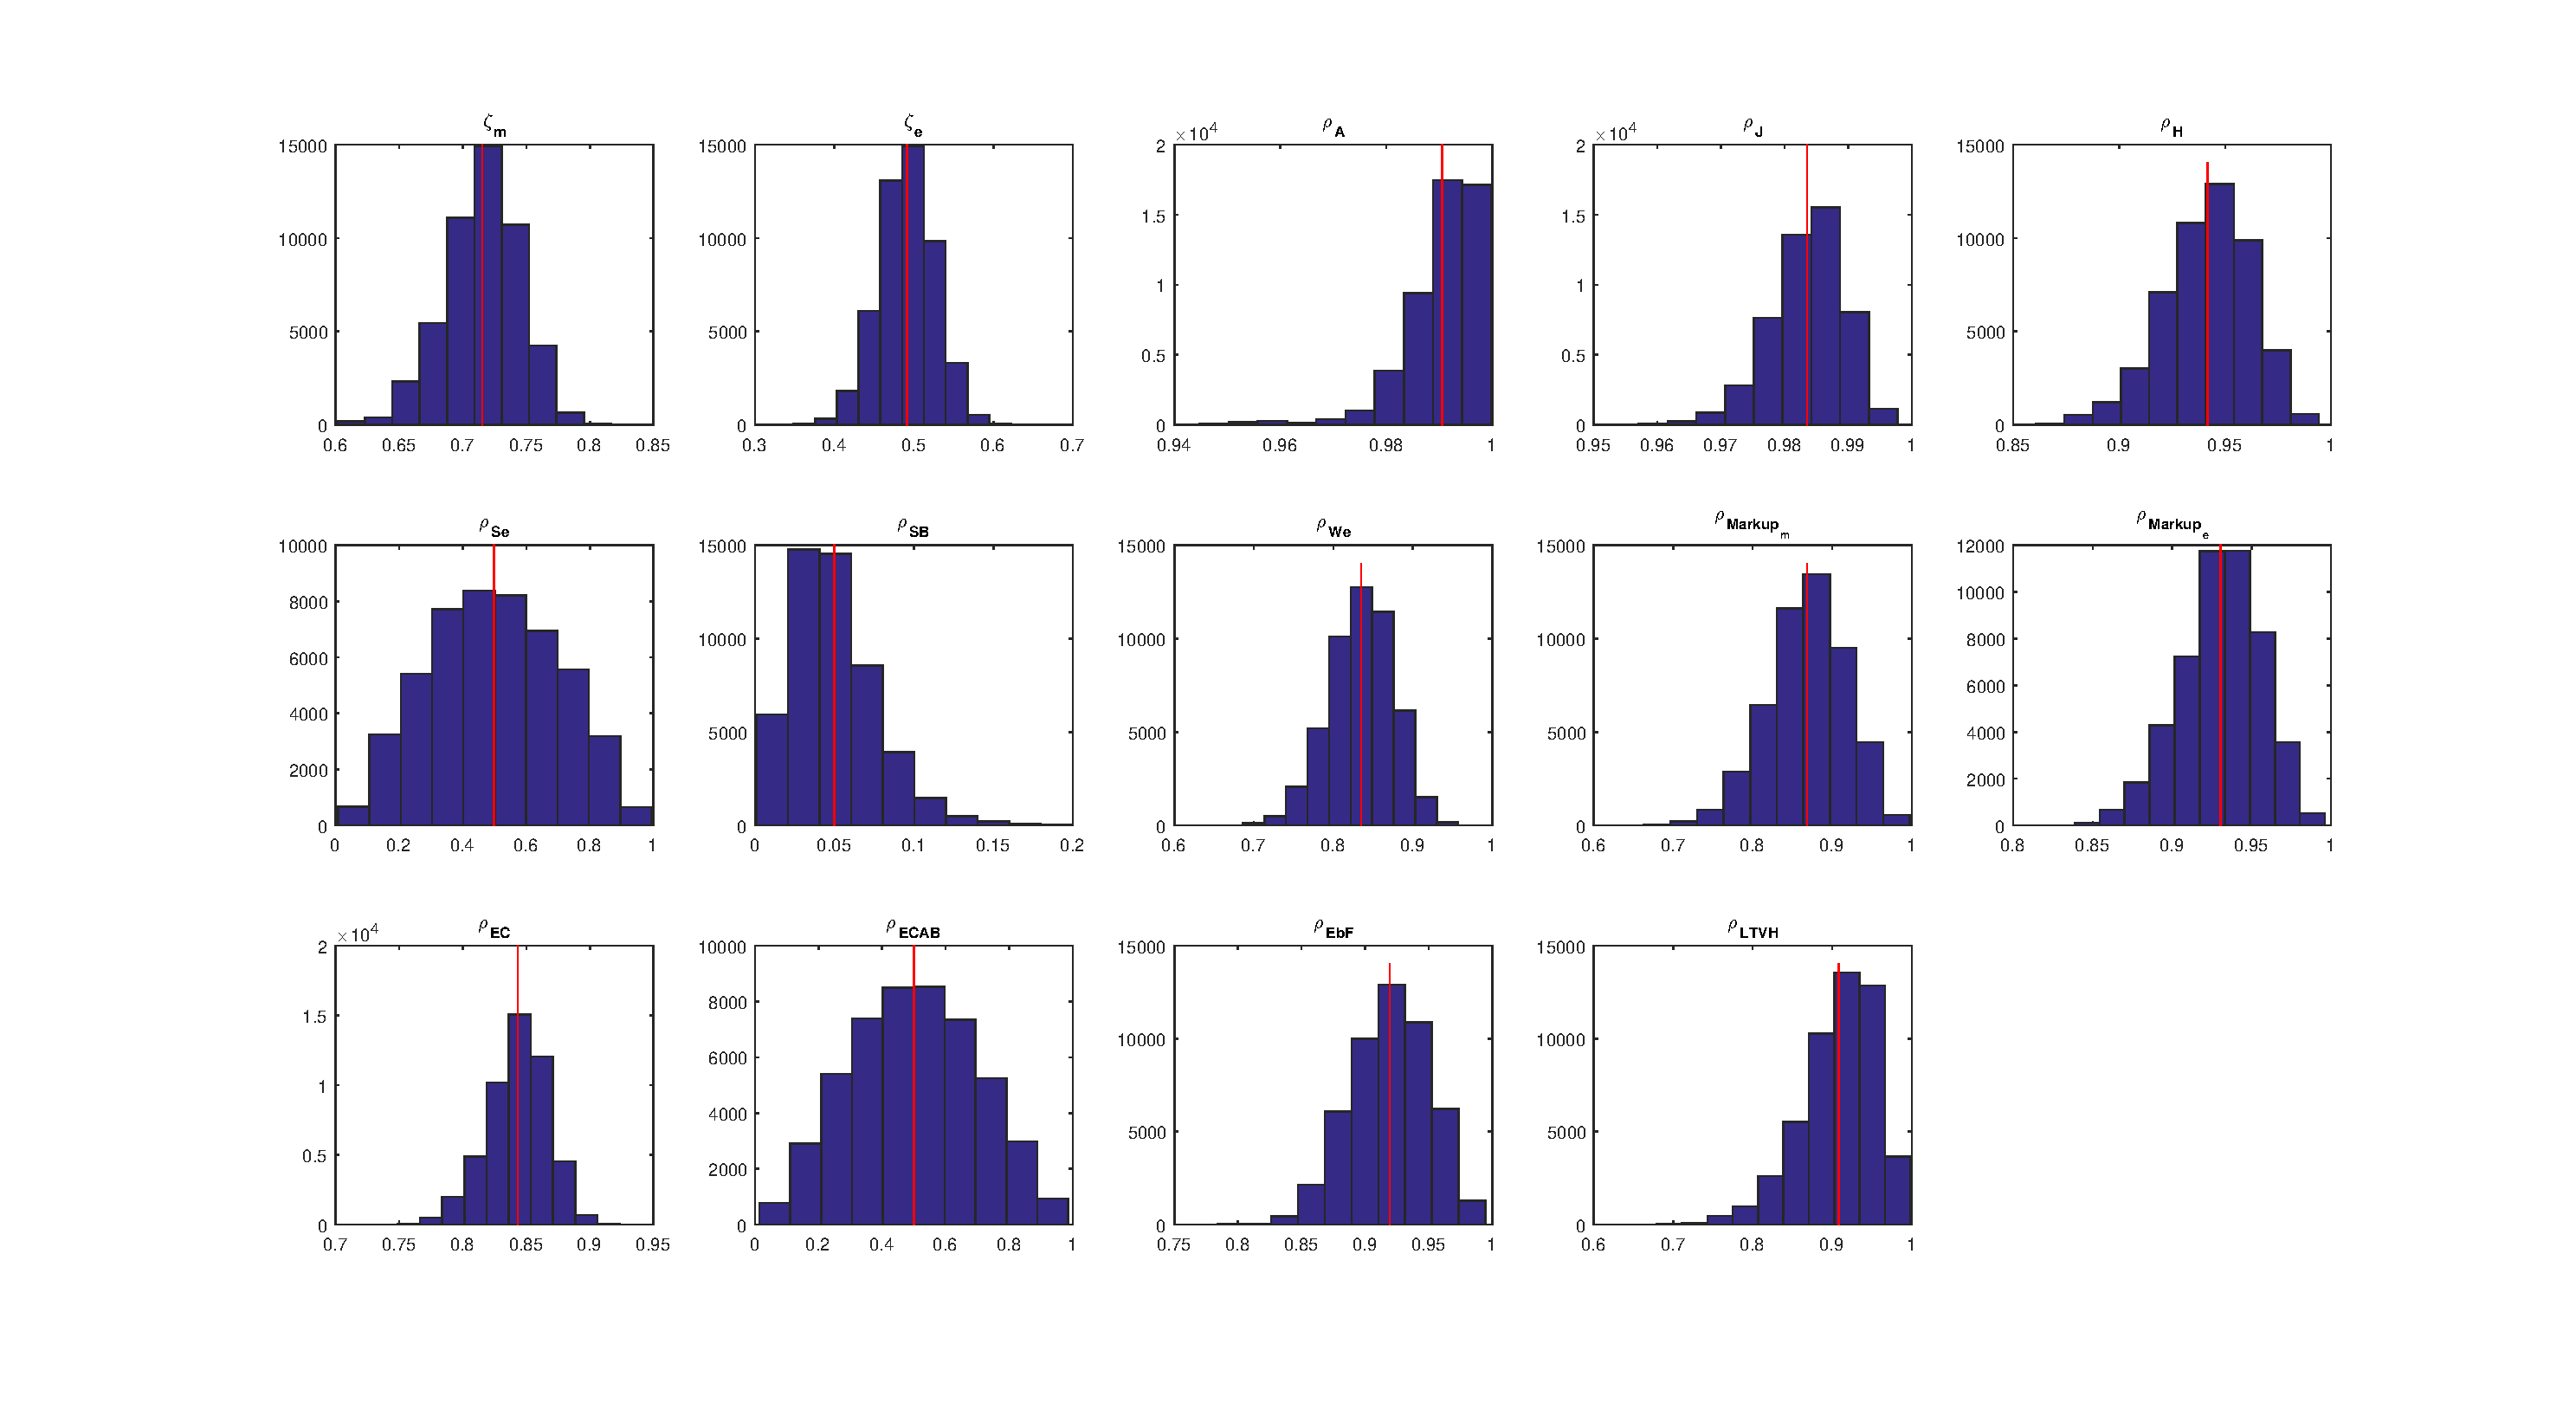
\includegraphics[scale=0.45]{posteriordistributions2.pdf}
\end{figure}

\FloatBarrier

\section{Model Overview and FOCs}
\label{app_modelOverview}
This is a infinite time horizon model with patient and impatient households.The other key agents in the model are entrepreneurs, banks,deposit insurance agency, final/investment/housing goods producers.

\subsection*{Households}

There are two types of households, patient and impatient, with patient households having a higher discount factor as in Iacoviello (2015).Both patient and impatient households have concave utility functions and derive utility from consuming goods, housing and leisure. The individual households are a part of a representative dynasty,which provides perfect risk sharing within the group. Thus, all individual households within the type are identical.Even if the individuals face idiosyncratic shocks, they are perfectly insured within their dynasty and hence consume and save/borrow identically.Both households supply labour in a competitive labour market.

\subsection*{Patient households}
In equilibrium, patient households are savers who hold deposit with banks and buy houses with their own funds. 

The objective function of the patient households (as is the case with impatient households) includes utility from consumption goods and housing and dis utility from labour.
\begin{equation}
\max_{c^s_t,L^s_t,D_{t},H^s_t}E_t\sum _{t=0}^{\infty } \beta_{s}^t [log(c^s_t)+vlog(H^s_t)-\frac{(L^s_t)^{1+\eta}}{1+\eta} ]
\end{equation}
This is subject to the following budget constraint:
\begin{equation}
c^s_t+q^H_{t}H^s_{t} +{D_{t}}=w_{t}L^s_{t}+q^H_{t}H^s_{t-1}(1-\delta)+{D_{t-1}}R^D_{t}+\pi_{t}
\end{equation}

The term $\pi_{t}$ includes profits of final goods producing firms and investment/housing production firms (which are owned by patient households), dividends from entrepreneurs and lumpsum transfers from deposit insurance agency. 

The FOCs for deposit and Housing stock is given by:

\begin{equation}
U'(c^{s}_{t}) = \beta_sE_t[ U'(c^{s}_{t+1})R_{Dt}]
\end{equation}

\begin{equation}
U'(c^{s}_{t})q^H = E_t[\beta_sU'(H^{s}_{t+1}) + \beta_sU'(c^{s}_{t+1})(1-\delta)q^H_{t+1}];
\end{equation}

\subsection*{Impatient households}

Impatient households borrow from banks using their houses as collateral as in Bernanke, Gertler \& Gilchrist (1999) . These mortgage loans are made on a limited liability non-recourse basis,  implying that individual households default whenever the value of the house is lower than the outstanding mortgage loans.The value of the house depends both on aggregate shocks (which affect house prices) as well as an idiosyncratic shock which determines whether an individual borrower defaults. In equilibrium, borrowers with an idiosyncratic shock below a certain threshold default.In the case of default, the bank takes possession of the houses in which case it is subject to state verification costs.

The borrowing is subject to LTV (Loan to value) limit set by the regulator. It is similar to a borrowing/collateral constraint as in Kiyotaki \& Moore (1997).

The objective function of the impatient households is the same as that of the patient households except for the discounting factor:
\begin{equation}
\max_{c^m_t,B^m_t,L_{t},H^m_t}E_t\sum _{t=0}^{\infty } \beta^t_{m} [log(c^m_t)+vlog(H^m_t)-\frac{(L^m_t)^{1+\eta}}{1+\eta} ]
\end{equation}

The budget constraint of impatient households reflects their borrowings under limited liability:
\begin{equation}
c^m_t+q^H_{t}H^m_{t} -B^m_{t}=w_{t}L^m_{t}+\int_{\bar{\omega^m_{t} }}^\infty  \left(\omega^m_{t} q^H_{t} H^m_{t-1} (1-\delta)B^m_{t-1}R_{t-1}\right) \, dF\omega^m_{t} + P_{t}
\end{equation}

The term under the integral reflects the limited liability of the borrowers as they default on their loans when the idiosyncratic shock $\omega^m_{t}$ is below the threshold level of $\bar{\omega^m}_t$. 

The default decision by the borrowers is given by:
\begin{equation}
{{\omega^m_{t} }}q^H_{t} H^m_{t-1}(1-\delta) <= B^m_{t-1}R^m_{t-1}
\end{equation}

The threshold level of $\bar{\omega^m}_t$ satisfies:
\begin{equation}
\bar{\omega^m}_t q^H_{t} H^m_{t-1}(1-\delta) = B^m_{t-1}R^m_{t-1}
\end{equation}


The LTV limit (or the borrowing constraint) is given by:
\begin{equation}
[B^m_{t}-(1-rp)B^m_{t-1}]R_{t} <=\epsilon_{t} E_t[q^H_{t+1} [H^m_t-H^m_{t-1}(1-\delta)]]
\end{equation}

where rp is the loan repayment rate and $\epsilon_{t}$ is the LTV limit.

The limit always binds in the steady state and it's neighborhood.

The FOCs for Mortgage loans and Housing stock is given by:

\begin{equation}
E_t{U'(c^{s}_{t})-\beta_m U'(c^{s}_{t+1})(R^m_{t}(1-def_{t+1}))-\lambda_{t}R^m_{t}+\lambda_{t+1}(1-rp)(1-def_{t+1})R^m_{t+1}=0}
\end{equation}
\begin{equation}
E_t{U'(c^{s}_{t})q^H = \beta_m U'(H^{s}_{t+1}) + \beta_sU'(c^{s}_{t+1})(1-Gm_{t+1})(1-\delta)q^H_{t+1}+\lambda_{t}(\epsilon_{t} q^H_{t+1})-\lambda_{t+1}(\epsilon_{t+1} q^H_{t+2})(1-\delta)}
\end{equation}

where def is the probability of default and the function Gm() represents the proportion of housing stock taken over by the bank for defaulted loans.$\lambda_{t}$ is the lagrange multiplier on the LTV constraint.




\subsection*{Entrepreneurs}

Entrepreneurs are risk neutral agents who own and maintain the stock of physical capital. They rent  capital to the final goods producing firms. Entrepreneurs derive utility from transferring part of their wealth to the saving dynasty (paying dividends) and retaining the rest for the next period (retained earnings). Entrepreneurs invest in capital goods and finance their investment by means of their own funds (net worth) and borrowings from banks. Similar to mortgage loans, these are limited liability non-recourse loans and hence subject to default by individual entrepreneurs in the event of value of assets falling below the outstanding loans.The value of the capital depends both on aggregate shocks (which affect house prices) as well as an idiosyncratic shock which determines whether an individual entrepreneur defaults. In equilibrium, borrowers with an idiosyncratic shock below a certain threshold default.  As in the case of households, assets are seized by banks and subject to costly state verification costs. 

\begin{equation}
\max_{K_t,B^e_t}E_t(W^e_{t+1})
\end{equation}	


\begin{equation}
W^e_{t+1}=max[\omega^e_{t+1}(r^k_{t+1}+(1-\delta)q^K_{t+1}K_{t})-R^F_{t}b^e_{t},0]
\end{equation}


The default decision of the entrepreneurs is given by:
\begin{equation}
{{\omega^e_{t} }}q^H_{t} K_{t-1}(1-\delta) <= K_{t-1}R^f_{t-1}
\end{equation}

The threshold level of $\bar{\omega^m}_t$ satisfies:
\begin{equation}
\bar{\omega^e}_t q^K_{t} K^m_{t-1}(1-\delta) = B^e_{t-1}R^f_{t-1}
\end{equation}
As borrowing is subject to LTV limit as follows:

\begin{equation}
[B^e_t-B^e_{t-1}(1-rp)]R^f_{t} =\epsilon_{t} E_t[q^F_{t+1} [K_t-K_{t-1}(1-\delta)]]
\end{equation}
Dividend rule:

A fixed proportion of wealth $\chi^e$ is paid out as dividends. This simple dividend paying rule for the entrepreneurs is given by:
\begin{equation}
c^e_t=\chi^e W^e_t
\end{equation}
As a result the retained earnings by the entrepreneurs is given by:
\begin{equation}
n^e_t=(1-\chi^e) W^e_t
\end{equation}

The balance sheet identity of the entrepreneurs is :
\begin{equation}
n^e_t+B^e_t=q^K_t K_t
\end{equation}

\subsection*{Bank}

Banks are financial intermediaries who channel savings from the savers to the borrowers.On the asset side of the banks, there are loans to households (mortgage lending) and entrepreneurs (business lending) respectively. As described earlier, these loans may default depending on aggregate state shocks and idiosyncratic borrower shocks in which case the banks seize the assets subject to state verification costs (these can also be viewed as bankruptcy costs).

On the liability side, there are deposits held by the patient households and equity capital held by the bankers. Deposits are insured by the Deposit Insurance agency. There is a capital adequacy requirement set by the regulator which along with a penalty cost function, which determines the amount of equity capital held by the bankers.

The key feature of the model is that banks may also default depending upon the performance of their loan portfolios (aggregate shocks) and idiosyncratic shocks (on similar lines as  the borrowers). The banks face an idiosyncratic shock to their returns on loans.Thus, in equilibrium, a fraction of banks below a certain threshold of the idiosyncratic shock level default. In case of default, the bank loan assets are also subject to possession  by the deposit insurance agency and costly state verification.

The banks' balance sheet identity is as follows:
\begin{equation}
n^b_{t}+D_{t}=B^m_{t}+B^e_{t}
\end{equation}

The maximization problem of the bank is given by:

\begin{equation}
\resizebox{1\textwidth}{!}{$
	\max_{R^{mi}_t,R^{fi}_t}E_t\sum _{t=0}^{\infty }\xi^t\beta_{s}^t [\{(1-G^H_{t+1}) (\widetilde{R^{mi}_{t}})(B^{mi}_{t})+(1-G^F_{t+1})\widetilde{R^{fi}_{t}}B^{ei}_{t}\}-(1-bankdef.prob){R^D_{t}}D_{t}+Penalty cost]$}
\end{equation}



\begin{equation}
\widetilde{R^{mi}_{t}}=(1-def.prob^m)R^{mi}_t+G^m_{t+1}(1 - \mu^m)( R^{mi}_t/\bar{\omega}^m_{t+1})
\end{equation}
\begin{equation}
\widetilde{R^{fi}_{t}}=(1-def.prob^e)R^{fi}_t+G^e_{t+1}(1 - \mu^e)( R^{fi}_t/\bar{\omega}^e_{t+1})
\end{equation}

The demand for Loans is given by:
\begin{equation}
B^{mi}_t=(\frac{R^{mi}_t}{R^{m}_t})^{-\tau} B^{m}_t
\end{equation}

\begin{equation}
B^{ei}_t=(\frac{R^{fi}_t}{R^{f}_t})^{-\tau} B^{e}_t
\end{equation}


Rmi/Rfi is the rate if interest charged by individual bank,$\tau$ is the elasticity of substitution between banks and determines their market power. $\mu$ is the proportion of state verification/bankruptcy costs.

\subsection*{Penalty cost function}

Penalty costs are modeled as a non pecuniary gain in utility if the capital adequacy ratio is higher than the minimum capital requirement and a non pecuniary cost if the capital adequacy ratio is lower than the minimum capital requirement.

\begin{equation}
Penalty cost_t=\nu^b \frac{[\frac{\phi^b_t}{\bar{\varphi_t}}]^{1-\sigma}-1}{{1-\sigma}}
\end{equation}

The above functional form,based on Nukhwoon \& Tsomocos (2018) builds in a non-linearity in the penalty costs.The marginal gains of having excess capital are decreasing whereas the marginal costs of having a shortfall in capital are increasing, whenever $\sigma$ is greater than 1. This creates an incentive for banks to maintain capital at a higher level as compared to the minimum regulatory requirement. In reality, we find that banks do maintain capital buffer over what is the minimum required.The parameter $\nu^b$ determines the weight attached to this penalty costs.

\subsection*{Interest rate stickiness}

Although, interest rate stickiness can be attributed to various reasons such as switching costs,menu costs, market structure, regulation etc.,we find the one of the main sources of interest rate sluggishness is the existence of fixed interest loans.

We introduce interest rate stickiness in a broader sense by modeling it as in Calvo (1983). This approach also has the benefit that it includes all possible sources of interest rate sluggishness in a reduced form (including the effect of long term fixed interest loans).It is assumed that only a $\xi$ proportion of banks are able to change their interest rates in a given period, whereas the remaining 1-$\xi$ proportion of banks are not able to change their interest rate. This staggered interest rate setting implies that the composite interest rate in the economy is an average of the current interest rate charged by the fraction of banks who can change the interest rate and the previous period interest rate.
To micro-found the staggered interest rate setting, we assume that there is imperfect competition in the banking sector. Banks offer differentiated loan products as in Gerali et al (2010) and are able to set their interest rate in the monopolistically competitive loan market.The borrowers takes a composite loan product comprising of all the aforesaid differentiated banking services.The composite interest rate paid by the borrowers is thus staggered on account of the Calco friction.In short,we extend the New Keynesian approach to goods market to the loan markets so as to generate interest rate stickiness. 

The FOCs for the interest rates are as follows.The FOC is similar to the FOC for price in a standard New Keynesian model with goods price stickiness:

\begin{equation}
R^{mi}_t=\frac{\tau}{\tau-1}\frac{E_t\sum _{t=0}^{\infty }\xi^t\beta_{s}^t MC_t}{E_t\sum _{t=0}^{\infty }\xi^t\beta_{s}^t rm_t}
\end{equation}
\begin{equation}
R^{fi}_t=\frac{\tau}{\tau-1}\frac{E_t\sum _{t=0}^{\infty }\xi^t\beta_{s}^t MC_t}{E_t\sum _{t=0}^{\infty }\xi^t\beta_{s}^t rf_t}
\end{equation}

\begin{equation}
MC_t=\lambda_{st+1}[(1-bankdef.prob)((1-\phi_t))R_{Dt}+\frac{\nu^b(\phi_t/\varphi_t)^{(1-\sigma)}}{(B^{mi}_t+B^{ei}_t)}](R^m_t)^\tau B^m_t
\end{equation}

As in the New Keynesian model with price stickiness, the interest rate charged by banks is a function of present discounted value (with the stickiness parameter) of present and future marginal cost times the mark up. The marginal cost includes the interest rate paid on deposits (in a competitive deposit market) and the penalty cost associated with the deviation from the regulatory capital requirement. The only difference from the standard New Keynesian version is the presence of borrower and bank defaults in the interest FOC for interest rate equation

\subsection*{Deposit Insurance Agency}

The deposit insurance agency insures the deposits. The assets of the defaulting banks are taken over by the agency and is subject to bankruptcy costs.The difference between the amount of deposits and the value of assets realized assets is recovered by the charging a lumpsum tax on households. 


\subsection*{Final goods producing Firms} 

There is a unit mass of perfectly competitive firms which combine capital and labour to produce the consumption good which is the numeraire.The firms rent capital from entrepreneurs. The firms are owned by patient households. They produce the final goods using a standard Cobb Douglas technology.

\begin{equation}
Y_{t}=A_{t} K^{\alpha}_{t-1}L^{1-\alpha}_{t}
\end{equation}

\subsection*{Capital goods and Housing production}

These are competitive firms which buy finished goods and produce capital goods /housing subject to quadratic adjustment costs.These firms produce new units of capital and housing using consumption goods which are then sold to entrepreneurs and households,respectively, at prices qK and qH. They represent the supply side of the capital goods/housing and pin down the equilibrium asset prices.These firms are also owned by the patient households.

They maximize their profits as follows:

\begin{equation}
\max_{I_t}E_t\sum _{i=0}^{\infty } \beta_{s}^t\{ \frac{c^s_t}{c^s_{t+1}}\} [q^K_{t+i} I_{t+i}-\{1+g[\frac{I_{t+i}}{I_{t+i-1}}]\} ]
\end{equation}

\begin{equation}
\max_{I^H_t}E_t\sum _{i=0}^{\infty } \beta_{s}^t \{ \frac{c^s_t}{c^s_{t+1}}\} [q^H_{t+i} I_{t+i}-\{1+g[\frac{I^H_{t+i}}{I^H_{t+i-1}}]\} ]
\end{equation}



\subsection*{Macro Prudential Policy}

The Macro Prudential policy pursued by the regulator includes a minimum capital requirement (also known as capital adequacy ratio) for the banks and a maximum loan to value ratio (LTV) for the borrowers. The regulator also sets a countercyclical capital rule which responds to the credit growth in the economy.

\begin{equation}
CR_{t}={\bar{CR}}+ \psi^{cr} log( B_{t}/{\bar{B}})
\end{equation}

The first part of the rule is the static minimum capital requirement which the banks are supposed to hold at any point of time. The second part is the counter cyclical component,which tracks the credit growth in the economy.

On similar lines,following is the rule for the LTV limit: 
\begin{equation}
LTV_{t}={\bar{LTV}}- \psi^{LTV} log( B_{t}/{\bar{B}})
\end{equation}



\end{appendix}


\end{document}
